\documentclass[print,nativefonts]{dissertation}

% chapter/cpaior-decoupling
\usepackage{amsmath}
\usepackage{amsthm}
\usepackage{algorithm}
\usepackage[noend]{algpseudocode}

\newcommand{\DP}{\textbf{\textsc{DP}}}
\newcommand{\TD}{\textbf{\textsc{TD}}}
\newcommand{\DU}{\textbf{\textsc{DU}}}
\newcommand{\OD}{\textbf{\textsc{OD}}}
\newcommand{\DTD}{\textbf{\textsc{DTD}}}
\newcommand{\BBox}{\rule{5pt}{6pt}}
\newcommand{\blbox}{ \hfill \BBox}
\newcommand{\var}[1]{\mathit{#1}}

\usepackage{mdframed}
%\newtheorem{mdexample}{Example}
%\newenvironment{example}%
%  {\begin{mdframed}[backgroundcolor=lightgray]\begin{mdexample}}%
%  {\end{mdexample}\end{mdframed}}
\newtheorem{example}{Example}[chapter]
\newtheorem{rquest}{Research Question}[part]


\newtheorem{observation}{Observation}[chapter]
\newtheorem{corollary}{Corollary}[chapter]
\newtheorem{proposition}{Proposition}[chapter]

% chapter/cpaior-stability
\usepackage{subcaption}
\captionsetup{compatibility=false}
\usepackage{amsfonts}
\usepackage{tikz}
\usetikzlibrary{arrows,automata}
\usetikzlibrary{arrows.meta}
%\usetikzlibrary{external}
%\tikzexternalize

\newcommand{\z}[1]{\mathcal{#1}}
\newtheorem{lemm}{Lemma}[chapter]
\newtheorem{exmp}{Example}[chapter]
\newtheorem{defn}{Definition}[chapter]
\newtheorem{obsv}{Observation}[chapter]

% chapter/mista-stability
\newcommand{\xsc}{\gamma}
\newcommand{\xSC}{\Gamma}

\newcommand{\xs}{\boldsymbol{s}}
\newcommand{\xd}{\boldsymbol{d}}
\newcommand{\xq}{\boldsymbol{q}}
\newcommand{\xb}{\boldsymbol{b}}
\newcommand{\xl}{\boldsymbol{l}}
\newcommand{\xf}{\boldsymbol{f}}
\newcommand{\xD}{\boldsymbol{D}}
\newcommand{\xt}{\boldsymbol{t}}

\newcommand{\xE}{\mathcal{E}}
\newcommand{\xS}{\boldsymbol{S}}
\newcommand{\xX}{\boldsymbol{X}}
\newcommand{\xP}{\boldsymbol{\Pi}}

% icaps flexibility
\newcommand{\est}{\ensuremath{\mathit{est}}}
\newcommand{\lst}{\ensuremath{\mathit{lst}}}
\newcommand{\flex}{\ensuremath{\mathit{flex}}}


% annotations
\usepackage{etoolbox}
\newtoggle{annotate}
\newcommand{\annotate}[1]{\iftoggle{annotate}{\subsection*{\textcolor{gray}{#1}}}\ }
\togglefalse{annotate}
%\toggletrue{annotate}

\usepackage{microtype}
%\usepackage{setspace} \spacing{1.15}
\usepackage{pgfgantt}
\usepackage{eurosym}
\usepackage{enumerate}


\begin{document}

%% Specify the title and author of the thesis. This information will be used on
%% the title page (in title/title.tex) and in the metadata of the final PDF.
\title[]{{Scheduling Under Uncertainty: Attaining Flexibility, Robustness and Stability}}
\author{Kiriakos Simon}{Mountakis}

%% Use Roman numerals for the page numbers of the title pages and table of
%% contents.
\frontmatter

\begin{titlepage}

\begin{center}

%% Extra whitespace at the top.
\vspace*{2\bigskipamount}

%% Print the title.
{\makeatletter
\titlestyle\bfseries\LARGE\@title
\makeatother}

%% Print the optional subtitle.
{\makeatletter
\ifx\@subtitle\undefined\else
    \bigskip
    \titlefont\titleshape\Large\@subtitle
\fi
\makeatother}

\end{center}

\cleardoublepage
\thispagestyle{empty}

\begin{center}

%% The following lines repeat the previous page exactly.

\vspace*{2\bigskipamount}

%% Print the title.
{\makeatletter
\titlestyle\bfseries\LARGE\@title
\makeatother}

%% Print the optional subtitle.
{\makeatletter
\ifx\@subtitle\undefined\else
    \bigskip
    \titlefont\titleshape\Large\@subtitle
\fi
\makeatother}

%% Uncomment the following lines to insert a vertically centered picture into
%% the title page.
%\vfill
%\includegraphics{title}
\vfill

%% Apart from the names and dates, the following text is dictated by the
%% promotieregelement.

{\Large\titlefont\bfseries Proefschrift}

\bigskip
\bigskip

ter verkrijging van de graad van doctor

aan de Technische Universiteit Delft,

op gezag van de Rector Magnificus prof.~dr.~ir.~T.H.J.J.~van der Hagen,

voorzitter van het College voor Promoties,

in het openbaar te verdedigen op woensdag 28 maart 2018 om 12:30 uur
%in het openbaar te verdedigen op (dinsdag 1 januari 2015 om 10:00 uur)

\bigskip
\bigskip

door

\bigskip
\bigskip

%% Print the full name of the author.
\makeatletter
{\Large\titlefont\bfseries\@firstname\ {\titleshape\@lastname}}
\makeatother

\bigskip
\bigskip

%Fachlehrer für Mathematik und Physik, \\
%Eidgenössische Polytechnische Schule, Zürich, Zwitserland,
Master of Science in Computer Science, Technische Universiteit Delft, Nederland,


geboren te Chania, Griekenland.

%% Extra whitespace at the bottom.
\vspace*{2\bigskipamount}

\end{center}

\clearpage
\thispagestyle{empty}

%% The following line is dictated by the promotieregelement.
\noindent Dit proefschrift is goedgekeurd door de

%% List the promotors (supervisors).
\medskip\noindent
\begin{tabular}{l}
    promotor: prof.\ dr.\ C.\ Witteveen \\
    copromotor: dr.\ T.B.\ Klos
\end{tabular}

\bigskip
\noindent Samenstelling promotiecommissie:

%% List the committee members, starting with the Rector Magnificus and the
%% promotor(s) and ending with the reserve members.
\medskip\noindent

\begin{tabular}{p{4.5cm}l}
    Rector Magnificus, & voorzitter \\
	 prof.\ dr.\ C.\ Witteveen, & Technische Universiteit Delft, promotor \\
    dr.\ T.B.\ Klos, & Universiteit Utrecht, copromotor \\

    \medskip
    \mbox{\emph{Onafhankelijke leden:}} & \\

    prof.\ dr.ir.\ K.I.\ Aardal, & Technische Universiteit Delft \\
	 prof.\ dr.ir.\ L.A.M.\ van Dongen, & Universiteit Twente \\
	 prof.\ dr.\ R.M.P.\ Goverde, & Technische Universiteit Delft \\
	 prof.\ dr.-ing.\ M.\ Papageorgiou,  & Technical University of Crete, Griekenland \\

    \medskip
    \mbox{\emph{Overige leden:}} & \\
    B.\ Huisman\ MSc & NedTrain, Utrecht \\
\end{tabular}

%\begin{tabular}{p{3cm}l}
%    Rector Magnificus, & voorzitter \\
%	 \mbox{prof.\ dr.\ C.\ Witteveen} & \\ & Technische Universiteit Delft, promotor \\
%    Dr.\ T.B.\ Klos, & Universiteit Utrecht, copromotor \\
%
%    \medskip
%    \mbox{\emph{Onafhankelijke leden:}} & \\
%
%    prof.\ dr.\ K.I.\ Aardal & Technische Universiteit Delft \\
%	 \mbox{prof.\ dr.ir.\ L.A.M.\ van Dongen} & \\ & Universiteit Twente \\
%	 \mbox{prof.\ dr.-ing.\ M.\ Papageorgiou} & \\ & Technical University of Crete, Griekenland \\
%	 \mbox{prof.dr.\ R.M.P.\ Goverde} & \\ & Technische Universiteit Delft \\
%
%    \medskip
%    \mbox{\emph{Overige leden:}} & \\
%    B.\ Huisman\ MSc & NedTrain, Utrecht \\
%\end{tabular}

%% Include the following disclaimer for committee members who have contributed
%% to this dissertation. Its formulation is again dictated by the
%% promotieregelement.
%\medskip
%\noindent prof.\ dr.\ ir.\ J.\ de Wit heeft in belangrijke mate aan de totstandkoming van het proefschrift bijgedragen.

%% Here you can include the logos of any institute that contributed financially
%% to this dissertation.
\vfill

\vspace{1.0cm}
\begin{minipage}[t]{0.25\textwidth}

\includegraphics[height=0.6in]{title/logos/nedtrain.pdf}
\end{minipage}
%
\begin{minipage}[b]{0.7\textwidth}
The research presented in this thesis has been funded by NedTrain in the framework of the applied Research \& Development Program `Rolling Stock Life Cycle Logistics'.
\end{minipage}
\vspace{1.0cm}

\vfill

\noindent
\begin{tabular}{@{}p{0.2\textwidth}@{}p{0.8\textwidth}}
	\textit{Keywords:} & {simple temporal network, flexibility, robustness, stability, scheduling under uncertainty, resource constrained project scheduling, monte carlo sampling} \\[\medskipamount]
	 \textit{Printed by:} & \textrm{Ridderprint BV} | \texttt{www.ridderprint.nl}
\end{tabular}

\vspace{4\bigskipamount}

\noindent Copyright \textcopyright\ 2017 by K.~S.~MOUNTAKIS

%% Uncomment the following lines if this dissertation is part of the Casimir PhD
%% Series, or a similar research school.
%\medskip
%\noindent Casimir PhD Series, Delft-Leiden 2015-01

%\medskip
%\noindent ISBN 000-00-0000-000-0

\medskip
\noindent An electronic version of this dissertation is available at \\
\url{http://repository.tudelft.nl/}.

\end{titlepage}



%% The (optional) dedication can be used to thank someone or display a
%% significant quotation.
\dedication{\epigraph{In loving memory of my father, Georgios Mountakis}{}}

\tableofcontents

\chapter*{Summary}
\addcontentsline{toc}{chapter}{Summary}
\setheader{Summary}


The research presented in this thesis is part of the \emph{Rolling Stock Life Cycle Logistics} 
applied research and development program, conducted by NedTrain.
As a company, NedTrain belongs to Nederlandse Spoorwegen (NS; the principal railway company in the Netherlands) and 
provides maintenance services for the NS train-fleet.
The aim of this program is to enhance NedTrain's competitiveness as a rolling-stock maintenance services provider.
Our work focuses on the operational aspects of this R\&D program,
motivated by the challenge of scheduling tasks (or operations) in a NedTrain maintenance workshop,
such that trains are delivered on-time for circulation in the rail network.
Most tasks in the workshop have uncertain durations (or processing times), which complicates the scheduling process. 

After introducing NedTrain as a company,
Chapter~1 identifies the main issues with scheduling in the workshop.  
The point is made that scheduling under uncertainty is not so much about finding a good (or timely) schedule,
as it is about continuously adapting to outcome task durations without violating scheduling constraints and without compromising timeliness.
Repeatedly changing the schedule of a workshop is not an option as it confuses and disorganizes human resources, thus impeding performance.
As such, we consider two options that management faces in order to cope with uncertainty:
i) instead of using a schedule that changes frequently, give people the flexibility to (re)schedule themselves at will;
ii) insert sufficient slack in the schedule to avoid frequent changes during task execution.
Each option above is mapped to a corresponding research problem shown below:
\begin{enumerate}[(I)]
\item{How to compute flexible schedules for independent work-teams that can be easily adapted to changes in the environment?}
\item{How to compute robust and stable schedules for work-teams in order to deal with uncertainty in the duration of maintenance tasks?}
\end{enumerate}


Pursuing option I above,
the aim is to provide as much flexibility as possible to independent decision-making parties in the workshop.
The main difficulty is ensuring scheduling constraints (i.e. precedences between tasks, due-dates, resource availability constraints)
will be satisfied by a schedule that is formed gradually from decisions taken independently by different parties.
The aim of pursuing option II, on the other hand, 
is to provide as much stability (i.e. a schedule that is not expected to change) as possible, 
without compromising performance (i.e. timely train deliveries).
The difficulty in pursuing option II is determining how much slack to insert and at which points in the schedule,
according to how uncertainty accumulates at different parts of the schedule.

Research Problem I is treated in Part I of the thesis.
In the tradition of earlier work in the context of RSLCL, 
we consider the research area of Simple Temporal Problem (STP) constraints.
The main idea behind our approach is modelling the situation in a NedTrain workshop (i.e. temporal and resource constraints) as an STP.
This STP is mapped into an interval schedule.
In contrast with a regular schedule (which prescribes a dispatching time per task),
an interval schedule prescribes a time-interval per task. 
So long as each task is dispatched within its time-interval,
constraint satisfaction in the workshop is guaranteed.

Part I is devoted to algorithms for finding a maximum flexibility interval schedule (prescribing as wide time-intervals as possible)
and for keeping it up-to-date with new information about already dispatched tasks, as it becomes available during execution.
Chapter~2 functions as a prelude to Part I.
The chapter begins with a summary of important concepts from STP-related literature.
It then shifts focus onto dentifying gaps in the literature which do not allow us to address Research Problem I.
Finally, a series of research ruestions associated with the gaps are formulated and these questions are addressed in Chapters~3 and 4.
Gaps in existing literature essentially stem from efficiency and dynamicity 
considerations that were not addressed by the earlier work of Wilson et al.
Here, we raise the following research questions:
\begin{enumerate}
	\item How to efficiently compute concurrent flexibility in a given STP, in low-order polynomial time?	
	\item How to incrementally recompute a concurrent flexibility interval schedule during dispatching?
	\item How to redistribute concurrent flexibility as fast as possible (using heuristic methods if necessary)?
\end{enumerate}

The method proposed by Wilson et al. for computing interval schedules of maximum concurrent flexibility
has an associated computation cost of $O(n^5)$ where $n$ is the number of tasks.
Since $n$ in the NedTrain case might be in the order of thousands, 
the first question above concerns the development of a more efficient interval schedule computation method.
The second and third questions, on the other hand, concern the addition of a dynamic dimension 
to the static concurrent flexibility framework originally developed by Wilson et al.
That is, they concern the development of methods for keeping the interval schedule up-to-date
with new information about already dispatched tasks.

Chapter 3 and the first part of chapter 4 address the first question.
Using a geometric interpretation of flexibility and using duality theory,
we show that the computation of flexibility can be cast as finding a min-cost matching on a weighted bipartite graph.
This allows us to compute flexibility in $O(n^3)$ with a min-cost matching algorithm (e.g. Hungarian method).
Therefore, improving upon the $O(n^5)$ bound associated with the Linear Programming (LP)-based approach originally proposed by Wilson et al.

Chapter~4 later goes on to addresses the second and third question.
Regarding the second question, it is shown how, given an interval schedule,
a new one can be computed every time a task gets dispatched at a point within the associated time-interval.
The flexibility available by the time-interval is longer needed after the task gets dispatched.
As such, we examine the problem of redistributing unused flexibility over yet-undispatched tasks.
Doing so allows us to continuously increase the flexibility per-task, as task execution unfolds.
To avoid causing confusion due to a continuously changing interval schedule,
every dispatching option available in the given schedule is also available in the updated schedule.
That is, time-intervals in the updated schedule contain those in the given schedule.
Redistributing flexibility (or updating the schedule) is effectively a rescheduling operation
and as such it should be computable with as much efficiency as possible, to keep pace with execution.
The last part of Chapter~4 concerns the development of a very efficient heuristic.


Research Problem II is treated in Part II of the thesis.
The main idea now is to model the situation in the workshop (i.e. temporal and resource constraints) as a stochastic task network,
i.e. a network of precedence relations between tasks with random durations.
Our main assumption is that we can estimate the probability distribution of each task duration based on historical data from past maintenance sessions.
Using this precise image of uncertainty in the workshop,
the task network is mapped into a predictive (or stable) schedule.
Human resources at the workshop are asked to simply dispatch tasks at the dispatching times prescribed in that schedule.
The predictive schedule is constructed with the right amount of slack at the right places,
such that it will remain mostly unchanged during task execution.

Part II is devoted to algorithms for finding such a stable predictive schedule
without compromising robustness (i.e. the chance of meeting train-delivery due-dates)
and (optionally) for adapting it to new information during task execution.
Chapter~5 functions as a prelude for Part II.
It begins with a summary of important concepts from the literature related to Stochastic Task Networks.
Gaps in the literature which do not allow us to address Research Problem II are identified,
leading to the formulation of a series of research questions associated with these gaps.
These questions are addressed in Chapter 6 and Chapter 7.
Here, we raise the following two research questions:
\begin{enumerate}
	\item How to optimize a scheduling policy and a predictive schedule together as a pair?	
	\item How to update the predictive schedule by reacting to outcome durations in low order polynomial time, keeping pace with execution?
\end{enumerate}

Though the predictive schedule is protected with the insertion of slack,
we cannot rule-out that a task will take more time than allocated (in the schedule).
A set of rules determining how to modify the schedule (if necessary) in such cases, is known as a scheduling policy.
In effect, the task execution process is guided by the predictive schedule in combination with the scheduling policy.
Prominent approaches in the literature consider optimizing the policy and the schedule separately.
In pursuit of potentially better results by performing optimization within a solution-space of higher dimensionality, 
the first question concerns optimizing schedule and policy together, as a single solution.
As noted above, outcome dispatching times might deviate from those in the predictive schedule.
In such cases, it might be beneficial to adjust slack allocation according to outcome dispatching times and task durations.
The second question concerns keeping the predictive schedule up-to-date with such new information as it becomes available during execution.
This being a rescheduling operation, emphasis is put on performing it with as much efficiency as possible.

The first question above is addressed in Chapter~6,
where we develop a two-step approach (optimizing schedule and policy separately, in two steps) 
and an integrated approach (optimizing policy and schedule together).
We accomplish this by developing a stochastic extension of existing MILP formulations 
for the (deterministic) Resource Constrained Project Scheduling Problem (RCPSP).
As expected, the integrated approach gives better results.
Unfortunately, however, it is too computationally expensive for problems of a practical size.
Our two-step approach, on the other hand, seems to be efficient and very effective at optimizing the predictive schedule
for a given scheduling policy, yielding better results than the state of the art.

The second question above is addressed in Chapter~7.
First we propose a LP for constructing a predictive schedule, based on a sample of random task durations.
This LP is costly to solve, with a complexity of $O(n^5 m^4)$ where $n$ is the number of tasks and $m$ is the size of the durations sample.
Targeting a specific part of the solution-space, 
we define an associated Simple Temporal Problem (STP) and show that an optimal 
predictive schedule can be constructed from the earliest-start-time solution of the STP.
Exploiting the special STP structure, we present our main result, 
a dynamic programming algorithm that finds an optimal predictive schedule with an associated cost of $O(n^2 m)$,
yielding considerable efficiency gains.
 
Chapter 8 concludes the dissertation.
First we assess our answers to the research questions.
Based on our answers, we proceed to discuss the degree to which Research Problems I and II have been adequately addressed.
We finish the chapter with a list of recommendations for future work.



\chapter*{Samenvatting}
\addcontentsline{toc}{chapter}{Samenvatting}
\setheader{Samenvatting}

{\selectlanguage{dutch}

Het onderzoek dat gepresenteerd wordt in dit proefschrift is onderdeel van Rolling Stock Life Cycle Logistics (Rollend Materieel Levenscycluslogistiek), 
een toegepast onderzoeks en ontwikkelingsprogramma, uitgevoerd door NedTrain. 
Nedtrain is een bedrijf dat behoort tot de Nederlandse Spoorwegen (NS, het voornaamste spoorwegbedrijf in Nederland) 
en biedt onderhoudsdiensten aan de treinvloot van de NS. 
Het doel van dit programma is om het concurrentievermogen van NedTrain te verbeteren als leverancier onderhoud service voor rollend materieel. 
Ons werk richt zich op het operationele aspect van dit R\&D-programma, 
gemotiveerd door de uitdaging van het plannen van taken (of werkzaamheden) in een onderhouds\-werkplaats van NedTrain, 
zodat treinen op tijd worden afgeleverd voor circulatie in het spoorwegnet. 
De meeste taken die in de werkplaats plaatsvinden hebben een onzekerheid in de duur (of verwerkingstijden), 
hetgeen het plannings\-proces bemoeilijkt.

Na de introductie van NedTrain als bedrijf, 
worden in Hoofdstuk 1 de belangrijkste problemen geïdentificeerd met betrekking tot plannen in de werkplaats. 
Het punt wordt gemaakt dat plannen onder onzekerheid niet zozeer gaat om het vinden van een goede (of tijdige) planning, 
maar om het voortdurend aanpassen van de planning aan de resulterende looptijden van de taken zonder de gestelde beperkingen 
in de planning te overtreden en zonder afbreuk te doen aan tijdigheid. 
De planning van de werkplaats herhaaldelijk wijzigen is geen optie omdat dat personeel zou verwarren en desorganiseren, 
en daarmee de prestaties belemmeren. Als zodanig beschouwen we twee mogelijkheden waar het management heeft om met de onzekerheid om te gaan: 
i) in plaats van een planning te gebruiken die vaak verandert, mensen de flexibiliteit te geven om zichzelf te (her)plannen naar believen; 
ii) voldoende speling in de planning toe te voegen om frequente wijzigingen tijdens de uitvoering van de taak te voorkomen. 
Elke bovenstaande optie is toegewezen aan een overeenkomstig onderzoeksprobleem dat hieronder is weer\-gegeven: 

\begin{enumerate}[(I)]
\item{Hoe flexibele plannen te berekenen voor onafhankelijke werkteams, plannen die gemakkelijk kunnen worden aangepast aan de veranderingen in de omgeving?}
\item{Hoe robuuste en stabiele planningen te berekenen voor werkteams om te kunnen omgaan met onzekerheid in de duur van onderhoudstaken?}
\end{enumerate}

Bij het nastreven van optie I hierboven, 
is het doel om zoveel mogelijk flexibiliteit te bieden aan onafhankelijke besluitvormende partijen in een werkplaats. 
De grootste moeilijkheid is ervoor te zorgen dat beperkingen op de planning 
(d.w.z. voorrang tussen taken, opleveringsdata, beperkingen op de beschikbaarheid van hulpbronnen) 
voldaan worden door een plan dat geleidelijk is gevormd door besli\-ssingen die onafhankelijk van elkaar worden genomen door verschillende partijen. 
Het doel van het nastreven van optie II, aan de andere kant, 
is om zoveel stabiliteit te bieden (d.w.z. een plan die naar verwachting niet zal veranderen) als mogelijk zonder afbreuk te doen aan prestaties (d.w.z. tijdige levering van treinen). 
De moeilijkheid in het nastreven van optie II is het bepalen van de hoeveelheid speling om in te voegen en op welke momenten deze in te voegen in het plan, 
afhankelijk van hoe onzekerheid accumuleert op de verschillende delen van het plan.

Onderzoeksprobleem I wordt behandeld in Deel I van het proefschrift. 
In de traditie van het vroegere werk in het kader van RSLCL, 
bekijken we op het onderzoeksgebied van Simple Temporal Problem (STP) beperkingen. 
Het belangrijkste idee achter onze aanpak is het modelleren van de situatie in een NedTrain-werkplaats (d.w.z. temporele beperkingen en beperkingen op de hulpbronnen) als een STP. 
Dit STP is toegewezen aan een intervalplan. 
In tegenstelling tot een regulier plan (dat een verzendtijd per taak voorschrijft), 
schrijft een intervalplan een tijdsinterval per taak voor. Zolang elke taak binnen zijn tijdsinterval wordt verzonden, 
is de voldoening aan de beperkingen in de werkplaats gegarandeerd.

Deel I is toegewijd aan argoritmen die een intervalplan van maximale flexibiliteit vinden (ze voorstellen zo breed mogelijk tijdsintervallen) 
en die dit plan bijwerken met de nieuwe informatie over de al verzonden taken naarmate deze informatie beschikbaar wordt tijdens uitvoering. 
Hoofdstuk 2 is een soort voorspel voor Deel I. 
Het hoofdstuk begins met een samenvatting van belangrijke concepten van de de STP-gerelateerde literatuur. 
Daarna richt het zich op het identificeren van de literetuugaten die ons niet toestaan om Onderzoeksprobleem I aan te pakken. 
Eindelijk formuleren we een reeks onderzoeksvragen die met de gaten te maken hebben, 
en we bekijken deze vragen in Hoofdstukken 3 en 4. 
De gaten in de bestaande literatuur komen in wezen voort uit de effictiviteit en dynamicity opzichten die niet bestudeerd werden in het vorige werk door Wilson et al. 
Hier stellen wij de volgende onderzoeksvragen:
\begin{enumerate}
	\item{Hoe kan men gelijktijdige flexibiliteit effeciënt berekenen in een gegeven STP, binnen een lage-orde polynomische tijd?}
	\item{Hoe kan men stapsgewijs een intervalplan van gelijktijdige flexibiliteit herberekenen tijdens het verzenden?}
	\item{Hoe kan men de gelijktijdige flexibiliteit zo snel mogelijk opnieuw verzenden (door middel van heuristieken, indien nodig)?}
\end{enumerate}

Wilson et al. hebben een methode bedacht om de interval plannen van maximum gelijktijdige flexibiliteit te berekenen, 
en deze methode neemt $O(n^5)$ tijd, waar n is het aantal taken. 
In het gevan van NedTrein, kan n in de orde van duizenden zijn, 
en daarom gaat de eerste vraag erboven over de ontwikkeling van een meer efficiënte intervalplannenmethode. 
Onderzoeksvragen 2 en 3, aan de andere kant, gaan over de toevoeging van een dynamische dimensie tot het statische gelijktijdige flexibiliteitskader, 
dat oorsproonkelijk door Wilson et al. geontwikkeld is. 
Deze vragen dus bekijken op de ontwikkeling van methoden voor het bijwerken van het intervalplan naarmate de nieuwe informatie over de al verzonden taken bekend wordt.

Hoofdstuk 3 en het eerste deel van Hoofdstuk 4 bestuderen de eerste vraag. 
Door middel van een geometrische interpretatie van flexibiliteit en met behulp van de dualiteitstheorie, 
demonstreren we dat de berekening van flexibiliteit kan worden geworpen als het vinden van een min-kost koppeling in een gewogen bipartiete graaf. 
Dit geeft ons de mogelijkheid om de flexibiliteit te berekenen binnen $O(n^3)$ door gebruik van een min-kost koppelingsalgoritme (bijvoorbeeld, de Hongaarse methode). 
Dat verbetert de $O(n^5)$ grens van de aanpak die gebaseerd is op Lineair Programmeren (LP), een aanpak die oorsproonkelijk Wilson et al. hebben voorgesteld.

Hoofdstuk 4 dan gaat door en nadert vragen 2 en 3. 
Wat vraag 2 betreft, er wordt laten zien hoe, gegeven een intervalplan, een nieuw intervalplan berekend kan worden elke keer dat een taak verzonden wordt op een punt binnen het betreffende tijdsinterval. 
De flexibiliteit beschickbaar in het tijdsinterval is niet meer nodig nadat de taak verzonden wordt. 
Daarom, bestuderen we het probleem van herverdeling van de niet verbruikte flexibiliteit naar de nog-niet-verzonden taken. 
Dit laat ons de flexibiliteit per-taak voortdurend verhogen, 
terwijl de taaksuitvoering zich ontvouwt. Om geen verwarring te veroorzaken door het voortdurend veranderende intervalplan, 
is elke verzendoptie die beschikbaar is in een gegeven plan ook in het bijgewerkte plan beschikbaar. 
Dat wilt zeggen, bevatten de tijdsintervallen van het bijgewerkte plan de tijdsintervallen van het gegeven plan. 
Het opnieuw verdelen van flexibiliteit (of het plan bijwerken) is eigenlijk een herplanningsoperatie, 
en daarom zou het berekenbaar zo efficiënt mogelijk zijn, 
om gelijke tred te houden met de uitvoering. 
Het laatste deel van Hoofdstuk 4 gaat over de ontwikkeling van een zeer efficiënte heuristiek.

Onderzoeksprobleem II wordt behandeld in Deel II van het proefschrift. 
Hier is het belangrijkste idee de situatie in de werkplaats modelleren (d.w.z. de temporale en hulpbronbeperkingen) als een stochastische taaknetwerk, 
d.w.z. een netwerk van voorrangrelaties tussen de taken met randomise duurtijden. 
Onze belangrijkste aanname is dat we de kansverdeling van elke taaksduur kunnen inschatten door middel van historische data van de onderhoudssessies van het verleden. 
Met gebruik van dit precieze beeld van onzekerheid in de werkplaats, 
wordt het taaksnetwerk toegewezen aan een voorspellend (of stabiel) plan. 
De mensen in de werkplaats worden gevraagd om de taken eenvoudig te verzenden op de verzendtijden die in dat plan staan. 
Het voorspellende plan wordt gemaakt met gebruik van de juiste hoeveelheid speling op de juiste plekken, 
zodat dat grotendeels hetzelfde blijft gedurende de uitvoering van de taken.

Deel II is gewijd aan algoritmen die zo’n stabiel voorspellend plan vinden zonder afbreuk te doen aan robuustheid (d.w.z. de kans van op tijd zijn met de treinaf\-leveringsdata) 
en (optioneel) die dat bijwerken naarmate nieuwe informatie komt gedurende de uitvoering van een taak.  
Hoofdstuk 5 speelt de rol van een voorspel voor Deel II. 
Het begint met een samenvatting van de belangrijke concepten van de literatuur over Stochastische TaakNetwerken (Stochastic Task Networks). 
We identificeren de gaten in de literatuur die het bekijken van Onderzoeksprobleem II onmogelijk maken, 
en dat brengt ons tot het formuleren van een reeks onderzoeksvragen die met deze gaten te maken hebben. 
Deze vragen zijn bestudeerd in Hoofdstukken 6 en 7. Hier stellen we de volgende twee onderzoeksvragen:
\begin{enumerate}
	\item{Hoe kan men een plannigsbeleid en een voorspellend plan samen optimaliseren als een paar?}
	\item{Hoe kan men het voorspellende plan bijwerken door op de resulterende looptijden te reageren binnen lage-orde polynomische tijd, terwijl we gelijke tred met de uitvoering houden.}
\end{enumerate}
Zelfs als het voorspellende plan beschermd is door het invoegen van speling, 
kan het gebeuren da een taak langer duurt dan gepland. 
Een verzameling regels die bepalen hoe het plan veranderd moet worden (als het moet) in zulke gevallen is bekend als een planningsbeleid. 
Eigenlijk, wordt het proces van taakuitvoeren geleid door het voorspellende plan samen met het planningsbeleid. 
De vooraan\-staande aanpakken in de literatuur werken afzondelijk aan het optimeseren van het beleid en het plan. 
In het nastreven van mogelijk betere resultaten door te optimeseren in een oplossingsruimte van een hogere dimensie, 
gaat de eerste vraag over hoe het plan en het beleid samen geoptimaliseerd kunnen worden, als een oplossing. 
Als we al hebben gemerkt, kunnen de tijden van het resultaatsverzenden afwijken van degenen in het voorspellende plan. 
Als dit het geval is, kan het volgende nuttig zijn: 
de spelingstoewijzing aanpassen volgens de verzendtijden van het resultaat en de looptijden van de taken. 
De tweede vraag gaat over het voorspellende plan bijwerkend houden naarmate zo’n nieuwe informatie beschikbaar wordt  tijdens de uitvoering. 
Omdat dit een herplanningsoperatie is, concentreren we op deze zo efficiënt mogelijk uit te voeren.

De eerste vraag hierboven wordt in Hoofdstuk 6 behandeld, 
waar we een aanpak van twee stappen (het plan en het beleid afzondelijk optimaliseren, in twee stappen) 
en een geïntegreerde aanpak (het beleid en het plan samen optimaliseren) ontwikkelen. 
Dat doen we door een stochastische extensie van de bestaande MILP formuleringen te ontwikkelen voor het (deterministische) 
Resource Constrained Project Scheduling Problem (RCPSP). 
Zoals verwacht, levert de geïntegreerde aanpak betere resultaten. 
Helaas, is het te rekenkundig duur voor problemen van praktische grootte. 
Aan de andere kant, lijkt onze twee stappen aanpak beiden efficient en heel effectief te zijn in het optimaliseren van het voorspellende plan voor een gegeven planningsbeleid; 
deze aanpak oplevert betere resultaten dan de state of the art.

De tweede vraag hierboven wordt in Hoofdstuk 7 behandeld. 
We stellen eerst een LP voor voor het opbouwen van een voorspellend plan, 
gebaseerd op een steekproef van randomise taaklooptijden. 
Dit LP is rekenkundig duur om op te lossen, met een complexiteit van $O(n^5 m^4)$, 
waar n het aantal taken betekend en m de grootte van de steekproef van de looptijden is. 
Met het oog op een bepaald deel van de oplossingsruimte, 
definiëren wij het erbij horende Simple Temporal Problem (STP) 
en we laten zien dat het optimale voorspellende plan gemaakt kan worden van de vroegste-begin-tijd oplossing van het STP. 
Door gebruik te maken van de speciale STP structuur, 
presenteren wij onze belangrijkste resultaat, 
een dynamisch programmeren algoritme dat een optimaal voorspellend plan vindt, 
een plan dat $O(n^2 m)$ kost, en dat aanzienlijke efficiëntiewinsten oplevert.

Hoofdstuk 8 rondt het proefschrift af. 
We beoordelen eerst onze antwoorden op de onderzoeksvragen. 
We gebruiken onze antwoorden om door te gaan en de mate van een geschikte behandeling van Onderzoeksproblemen I en II te discusseren. 
We sluiten het hoofdstuk af met een lijst aanbevelingen voor toekomstig werk.


}


\chapter*{Preface}
\addcontentsline{toc}{chapter}{Preface}
\setheader{Preface}

This book marks the ending of my journey as a Ph.D. student with the Algorithmics research group of TU Delft. 
As an experience, it has been rather gratifying and rewarding but also very challenging at times. 
This book would not exist without the substantial support of my supervisors, 
which I have been receiving ever since I started working with them, initially as a MSc student.
Cees Witteveen, Tomas Klos, and Bob Huisman, 
thank you for giving me the opportunity to grow both as a scientist and a person under your supervision.

In turn, I would like to thank my family and my Sophie for their support and 
guidance that enabled me to maintain faith during the more challenging periods of this journey. 
In addition, I would like to thank Tim and Gleb for their friendship and support
and for long insightful discussions over various topics.
I am also grateful to my colleagues in the Algorithmics group for the ‘gezelligheid’ during lunch.
Finally, I am thankful to my predecessor, Michel, 
whose name is often cited in this book since his work set the foundation for many of the results presented here.

With a combination of pride and other feelings, 
I welcome the transition to a new phase of my life and I’m looking forward to whatever lies ahead.
 
\begin{flushright}
{\makeatletter\itshape
    \@firstname\ \@lastname \\
    Chania, November 2017
\makeatother}
\end{flushright}



%% Use Arabic numerals for the page numbers of the chapters.
\mainmatter

%% Turn on thumb indices.
%\thumbtrue

\chapter{Introduction}
\label{chapter:introduction}
% intro to chapter

	The subject of this thesis is inspired by a real scheduling problem as experienced by the NedTrain company.\footnote{http://www.nedtrain.nl}
	After a general introduction to the NedTrain company, we identify two main problems in scheduling for maintenance 
	engineering which according to our view are not only problems this particular company is facing, 
	but also are of general interest for the research field of scheduling.
	After a description of these research problems, 
	in subsequent chapters we derive some scientific research questions from these research problems and analyse them in full detail.  

\section{NS Group and NedTrain}

	% NS Group and its different parts
		NedTrain is a subsidiary company of Nederlandse Spoorwegen (NS) Group\footnote{http://www.ns.nl}, 
		the principal Dutch railway operator, 
		the origins of which can be traced back to the begining of the 19-th century.
		NS, which in 2016 made close to 90\% of their revenue from passenger trasport,
		serves approximately 1 million passengers per day mainly in the Netherlands but also in Germany, 
		the United Kingdom (UK) and other parts of Europe \cite{NS2016}. 
		Figure~\ref{fig-ns} shows the group of companies composing NS: 
		NS~Reizigers (or NSR, with approximately 11,000 staff), NedTrain (3,000), 
		NS~Stations (5,000, including retail) and Abellio (13,000).

		\begin{figure}
			\centering
			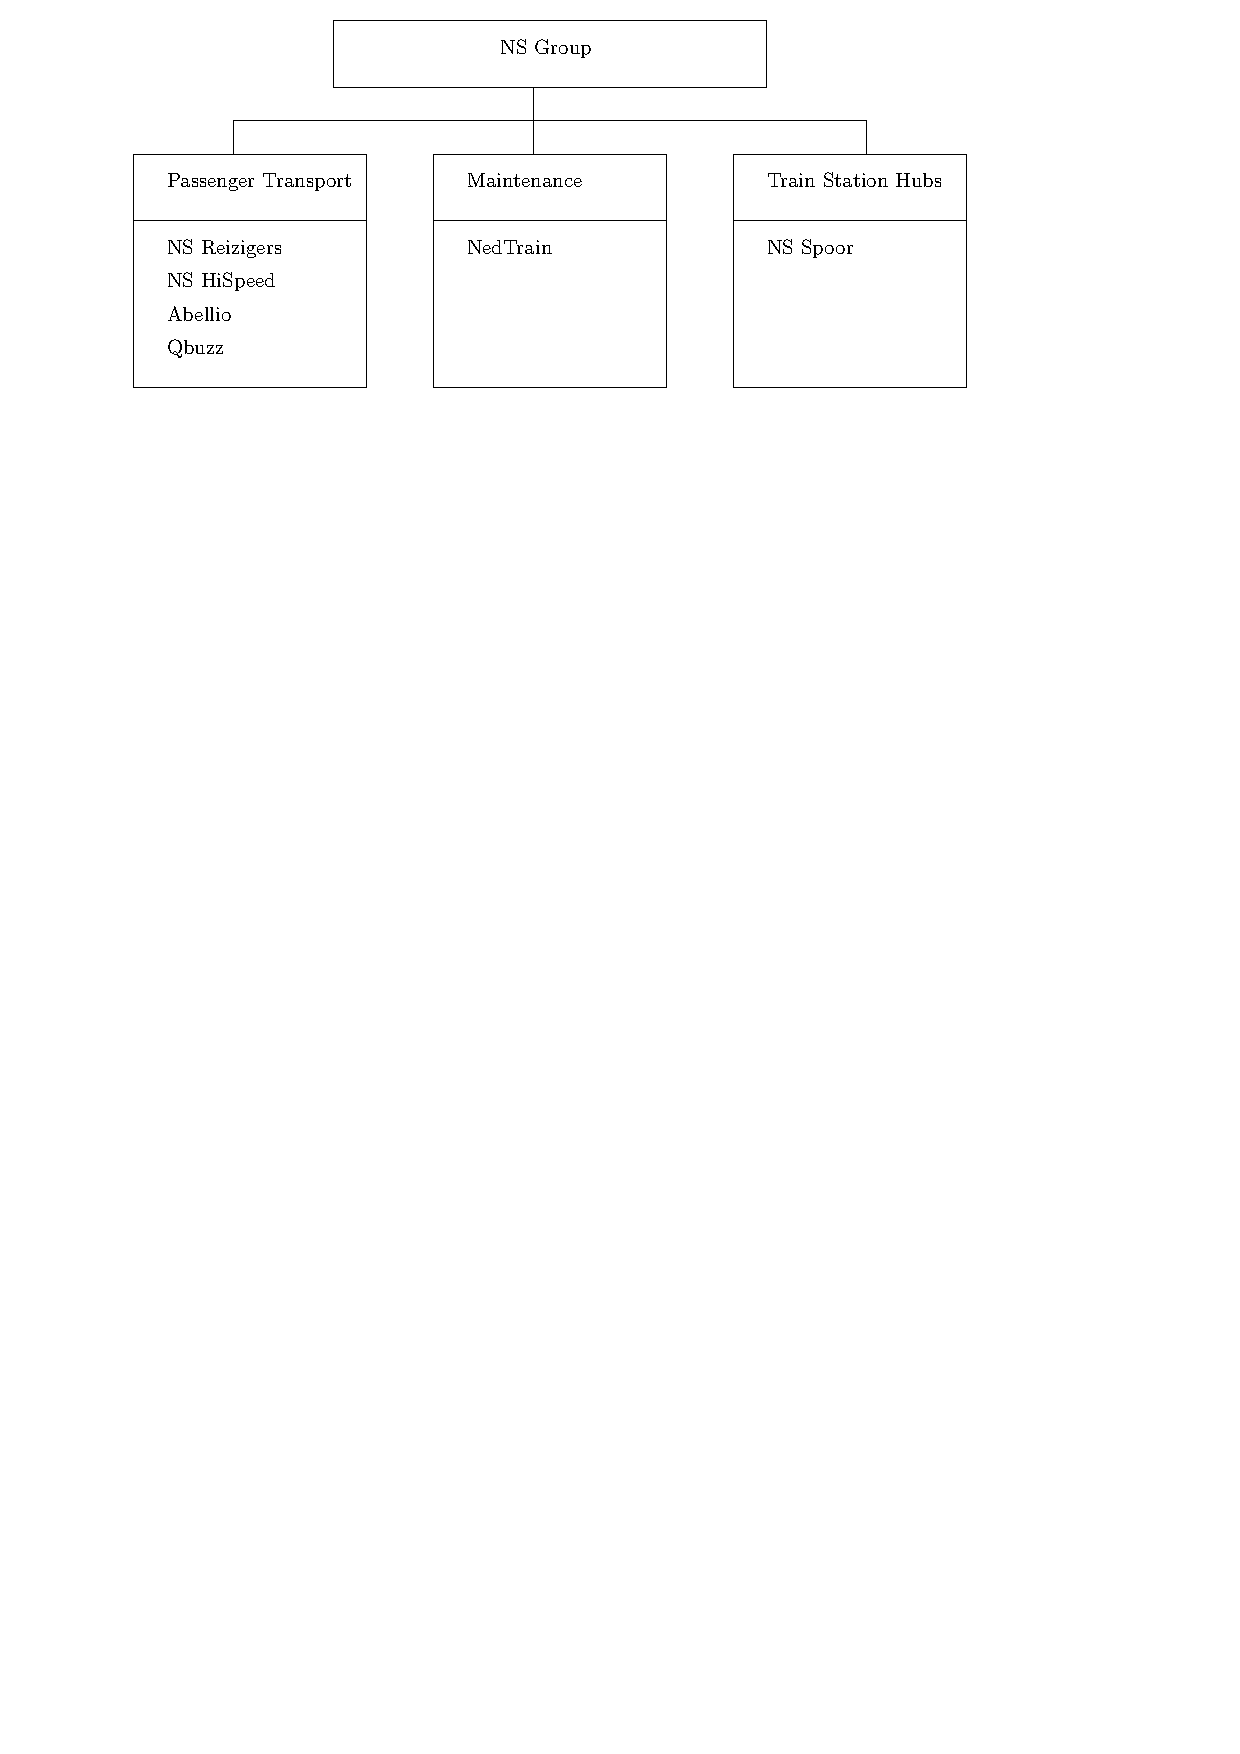
\includegraphics[width=0.95\textwidth]{chapter/introduction/ns-structure}
			\caption{NS Group and subsidiary companies (adapted from \cite{NS2016}).} 
			\label{fig-ns}
		\end{figure}

		% about NS Reizigers and NS Highspeed
		NS Reizigers and NS International operate the majority of trains on the Dutch rail network.
		They handle domestic and international passenger transportation, respectively,
		with a fleet of approximately 3000 rolling-stock units.
		Abelio handles passenger transportation in the UK and in Germany.
		% about NS stations
		NS Stations handles the development and operation of 410 large and small train stations,
		in cooperation with ProRail which is the company managing the Dutch rail network (not part of NS Group).

	% NedTrain; first-line service, technical maintenance and refurbishment
		NedTrain is responsible for maintaining a high availability rate for NS Reizigers and NS International trains, 
		providing the following types of maintenace: 
		\begin{description}
			\item[First-line service] 
			First-line service involves a daily cleaning and fixing of small technical problems 
			of each train at least once a day at one of thirty `servicebedrijf' (SB) facilities throughout the country. 

			\item[Technical maintenance]
			Once every three months or after a critical part has reached a certain mileage 
			each train goes to one of four NedTrain workshops, or `onderhoudsbedrijf' (OB) facilities for technical maintenance. 

			\item[Refurbishment] 
			Once or twice in its lifetime, a train might have to be refurbished to meet modern standards, 
			and refurbishment takes place in an overhaul and refurbishment workshop, in Haarlem.
		\end{description}
	% NedTrain: technical maintenance; the weekly schedule
		The work presented in this dissertation deals with scheduling problems 
		related to technical maintenance operations in a NedTrain workshop.
		NedTrain has four workshops for technical maintenance in The Netherlands: 
		in Amsterdam, Leidschendam, Onnen and Maastricht, and each location specializes in specific train types 
		(Figure~\ref{fig-workshop-1},\ref{fig-workshop-2}).
		Each workshop operates non-stop, 24 hours a day, covered by three 8-hour personnel shifts.
		For each workshop there is a week-long ``abstract'' schedule that mostly stays the same throughout the year.
		This schedule specifies when and which types of trains are expected to arrive at the workshop 
		and also when they must be returned for circulation in the rail network.
		This week-long abstract schedule is designed in harmony with the week-long time-tables used by NS Reizigers to carry passengers
		and such that NedTrain handles an evenly distributed workload over the year.

		Even though the abstract schedule stays more-or-less fixed throughout the year,
		the scheduling problem to be dealt with in a workshop changes on a weekly basis.
		This is because the list of necessary maintenance tasks for each specific train-fleet unit depends 
		on its past visits at the workshop and on its current condition.
		That is, each week the workshop operates based on an instantiation of the abstract schedule, 
		depending on the particular train units that will arrive for maintenance.
		In other words, the abstract schedule simply specifies arrival and due-dates for types of trains, 
		since from a passenger service point-of-view,
		it is only important that some train unit of a specific type is available when needed.

		About two weeks prior to an upcoming week, knowledge about which specific trains will arrive at the depot becomes available. 
		Each train is expected to arrive on a respective \emph{release-date} and 
		it must be delivered for circulation before a respective \emph{due-date}.
		If train constitutes a maintenance project then multiple projects will typically execute in parallel at the workshop.
		Depending on weather conditions and other factors, the number of trains under technical maintenance in 
		NedTrain workshops at the same time might peek to 300, i.e. to about 10\% of the entire fleet. 
		With about 50 tasks per train on average,
		up to 1500 tasks with uncertain durations might be taken into consideration when creating a weekly workshop schedule.
		
\section{NedTrain's Research \& Development program}

	NedTrain has the ambition to be a first class European rolling stock maintenance company. 
	To support their ambition, NedTrain intiated the `Rolling Stock Life-Cycle Logistics' (RSLCL) 
	applied research and development program, in cooperation with several Dutch universities.
	The main question to be addressed by the RSLCL program can be formulated as follows:
	\begin{quote}
		How to obtain and maintain the best combination of rolling stock, maintenance
		operations and supply chain, within the context of railway operations, to enable
		our customers to deliver competitive high quality services to their passengers? \cite{huisman2009}
	\end{quote}

	The search for an answer to this question is mostly directed by the following
	Key Performance Indicators (KPIs) concerning the train-fleet of NS:
	\begin{enumerate}
		\item total Cost of Ownership (or Life-Cycle Cost) of the fleet;
		\item availability of sufficient transport capacity;
		\item reliability of transport;
		\item quality of transport.
	\end{enumerate}
	
	The scope of the RSLCL program is too wide to be undertaken as a single study.
	As such, the program has been divided into three different levels:
	the strategic, tactical and operational level,
	each associated with a different time-scale of planning and control.
	In what follows we give a summary for each of the three levels of the program.
	
	\begin{description}
	\item[Strategic]
	Since rolling stock has several decades of life-time,
	decisions regarding the acquisition of rolling stock constitute long-lasting investments that tie up resources for years.
	Moreover, buying rolling stock amounts to less than 40\% of the overall life-cycle cost.
	That is, most money is spent on operation and maintenance during the years rolling stock is in service.
	Since this amount of money is mostly allocated during the acquisition process,		
	the main objective at the strategic level is the development of methods for
	ranking acquisition options from the perspective of \emph{supportability} and the design optimal logistics support.
	
	\item[Tactical]
	The tactical level concerns the allocation and planning of spare parts, 
	human resources and maintenance tasks and the management of physical flows,
	given that decisions about the acquisition of rolling stock 
	and the maintenance infrastructure have been made and will remain fixed on the intermediate timescale.
	Moreover, the tactical level considers the impact of changing the supply chain in order to
	outsource some of the maintenance operations to the manufacturer of rolling stock.
	
	\item[Operational]
	The operational level concerns the effective scheduling of maintenance operations in a NedTrain workshop,
	in order to ensure timely delivery of rolling stock for circulation in the rail network.
	Maintenance tasks having uncertain durations
	(partly because of the conditional nature of repairs, i.e. not knowing which repairs must be performed until
	after the arrival and inspection of a train in the workshop) makes the scheduling of technical maintenance a rather challenging feat.
	Due to the possibility of maintenance running late,
	ensuring a certain level of fleet availability relies on buffer stock.		
	The main objective at the operational level is to reduce the total cost of fleet ownership
	by improving the planning and scheduling process at the workshop,
	which in turn would allow the level of buffer stock to decrease.	
	\end{description}
	 
	In a joint cooperation with the technical universities in the Netherlands, 
	three research projects have been carried out:
	Research concerning the strategic level has been conducted by Parada Puig et al. \cite{parada:2015} at the University of Twente and
	research concerning the tactical level has been conducted by Arts et al. \cite{arts2013spare} at the Technical University of Eindhoven.
	Research concerning the operational level is undertaken by Wilson et al. \cite{wilson:2016} at the Technical University of Delft.
	As a follow-up to the work of Wilson et al., this dissertation also focuses on the operational level,
	i.e. the scheduling of maintenance tasks in a NedTrain workshop, in the face of uncertainty.		
	%
	% TODO: what michel achieved wrt scheduling
	% Here is a slight gap: you have to mention what the essential contribution is of Michel’s thesis and what he left open.
	% he did not pay attention to uncertainty
	%
	The overall research effort concerning all three levels of the program 
	is monitored and directed at regular Steering Group meetings
	that take place (up to) four times a year, involving a representative for each of the stakeholders.
	
	In what follows we focus on the current scheduling process at NedTrain
	and highlight the basic issues caused by the presence of uncertainty.
	Moreover, we propose two potential approaches for better dealing  with uncertainty
	and formulate corresponding research problems that we will be addressing in our work.

\section{Basic issues with maintenance scheduling}
	% workshop pictures
		\begin{figure}
			\centering
			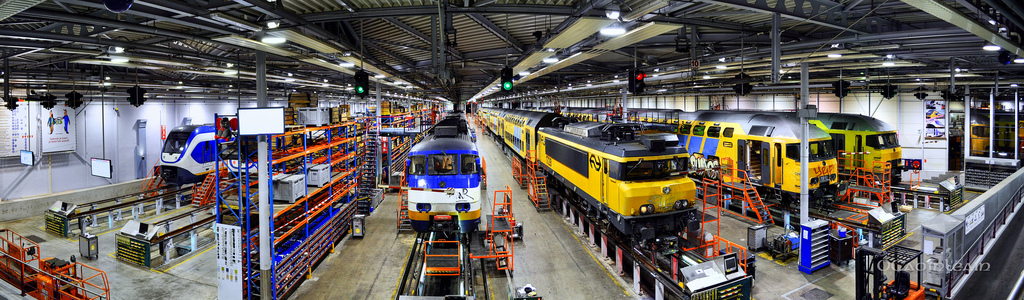
\includegraphics[width=0.9\textwidth]{chapter/introduction/workshop-1}
			\caption{Inside the Leidschendam workshop.}
			\label{fig-workshop-1}
		\end{figure}

		\begin{figure}
			\centering
			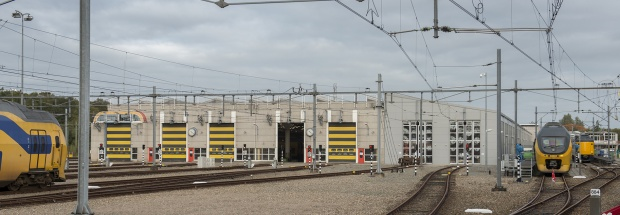
\includegraphics[width=0.9\textwidth]{chapter/introduction/workshop-3}
			\caption{Shunting yard of the workshop in Onnen.}
			\label{fig-workshop-2}
		\end{figure}

	% what is the complication
		As with most (if not all) real-life applications of scheduling,
		the main complication in NedTrain's case is that tasks have uncertain durations.
		In a maintenance workshop, dismounting parts is a very common operation.
		In contrast with assembling a part (as in production), the time needed for a dismount tends to vary according to uncontrollable factors.
		Another source of uncertainty is due to the conditional nature of repairs.
		That is, some tasks involve inspecting a certain part and then repairing it, if necessary.
		The duration of such tasks is by definition highly uncertain since whether 
		any time will be spent on repairing the part is unknown in advance.

		A schedule, on the other hand, is created subject to temporal and resource constraints and allocates a fixed amount of time per task.
		If the amount of time needed (i.e. the outcome duration) exceeds the amount of time allocated for a task (i.e. the predicted duration),
		then some other tasks might have to be rescheduled in order to comply with temporal constraints and/or resource constraints.
		As a result, scheduling in an uncertain environment is not so much about finding a good schedule 
		as it is about keeping the schedule up-to-date with outcome durations without deteriorating its quality in the long run.

	% what is done now
		Currently, the scheduling process at NedTrain is semi-automated.
		A baseline schedule is created and adapted during task execution as necessary by a team of 
		planners who rely on their domain expertise and the help of software like ProPlan or Microsoft Excel.
		To cope with uncertainty, a significant amount of slack is inserted in the schedule.
		Moreover, as a last resort option, some tasks might be skipped and postponed for the next workshop visit in order to deliver a train on time.

	% the difficulty of slack insertion
		Adding too much slack stabilizes dispatching times (meaning they will probably not change much during task execution) 
		but at the same time it compromises efficiency or punctuality, because the schedule becomes long.
		Adding too little slack, on the other hand, means we will have to update the schedule often during execution.
		Aggressive and frequent rescheduling of human resources is highly undesirable as it creates confusion, or nervousness, 
		which in the end also hinders performance.
	
	% how to improve the current approach
		In the NedTrain workshop we are dealing with large scheduling problems 
		with several hundreds of tasks and constraints and a great deal of uncertainty.
		The demand to keep the schedule up-to-date with a changing environment without introducing confusion, 
		or ``shop-floor nervousness'' while achieving a high degree of timeliness,
		might easily outstrip the capacity of human planners.
		The current approach works but there is clearly room for improvement, as we see more in detail in the next section.
		The mission of NedTrain's R\&D, at the operational level, 
		is to modernize the scheduling process by finding state-of-the-art scheduling techniques 
		that can be adapted and/or extended for the particular requirements of the NedTrain workshop.
		Based on eventual research findings, the purpose is to develop custom-tailored scheduling tools that can help 
		operational planners to enhance punctuality and eliminate nervousness at the workshop, without sacrificing throughput.

	% repair picture
		\begin{figure}
			\centering
			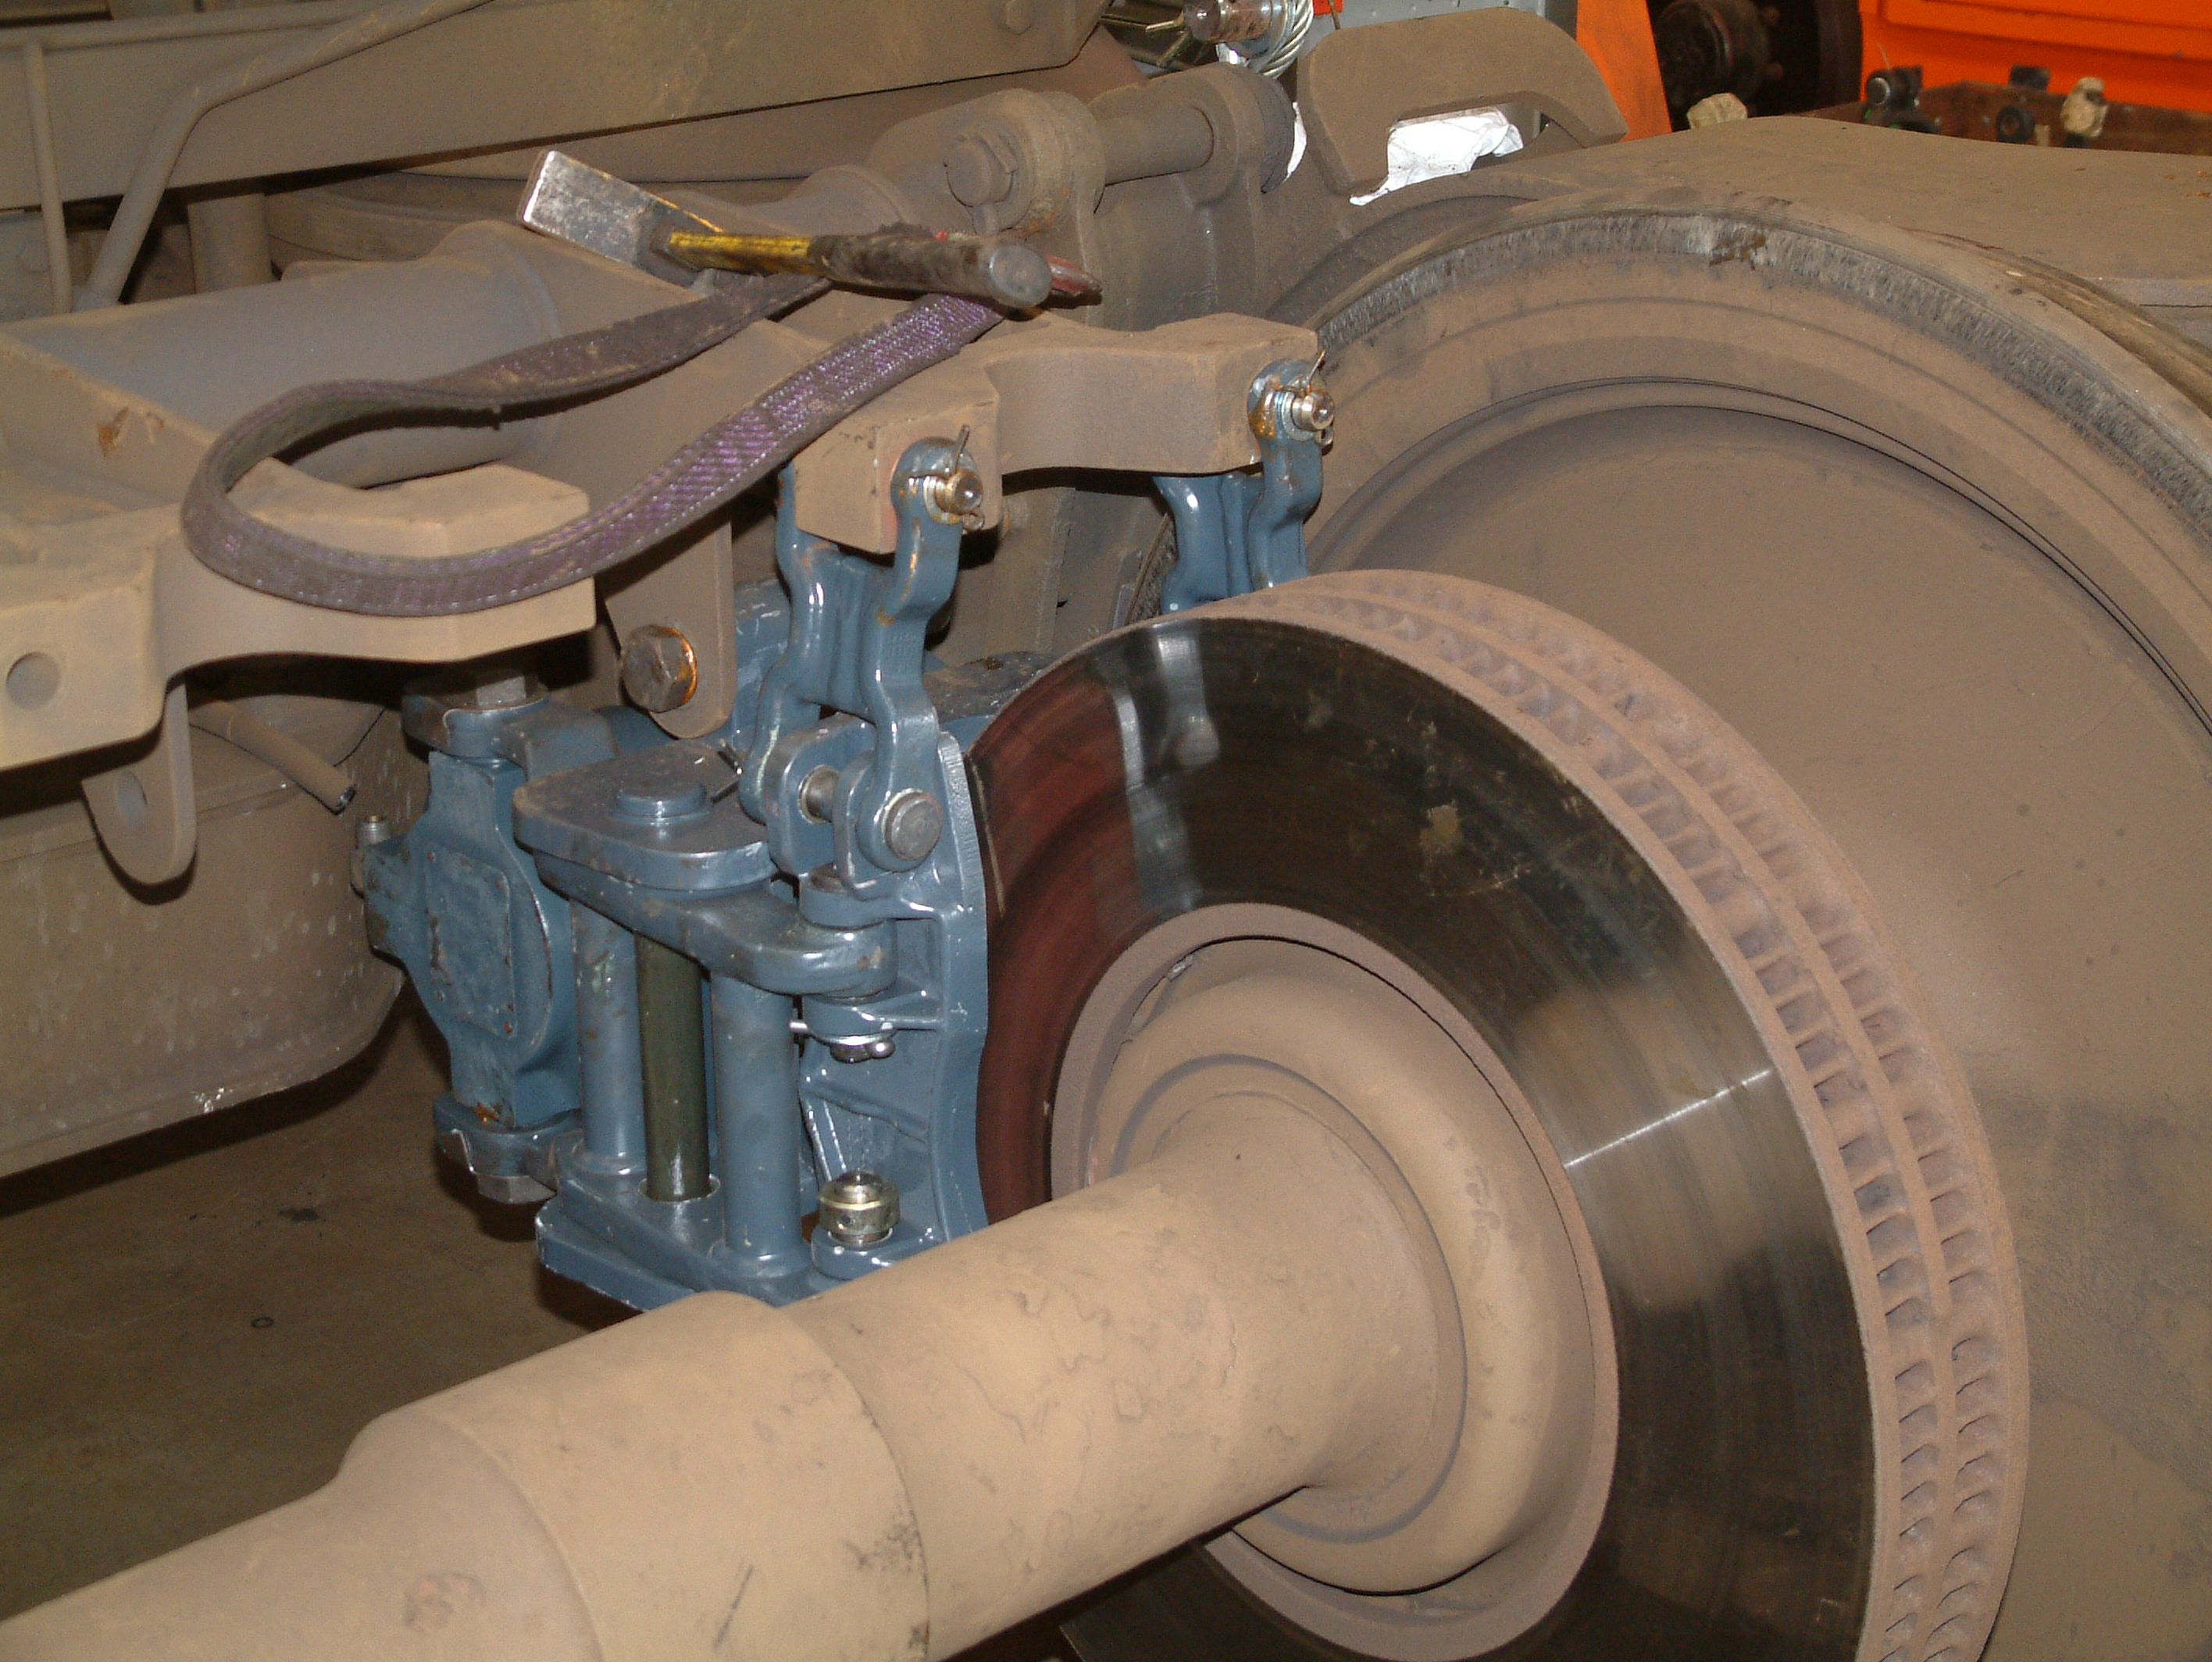
\includegraphics[height=0.3\textheight]{chapter/introduction/workshop-4}
			\caption{Replacement of a faulty part.}
			\label{fig-workshop-4}
		\end{figure}

\section{Research Problems}
\label{chapter:introduction:research-problems}

	% the two options of management
		Since human resources are very much against the idea of being rescheduled frequently,
		management has to choose between two options: 
		\begin{enumerate}[(I)]
			\item Adding sufficient slack to avoid the need for continuous rescheduling (nervous process), or
			\item give human resources the autonomy to take the decisions to (re)schedule themselves.
		\end{enumerate}
		In other words, unless management is able to provide a schedule that remains stable (i.e. relatively unchanged) during execution,
		people would rather have the freedom to (re)schedule themselves and stay in control.

	% what it means to pursue option 2
		Pursuing option two (letting people reschedule themselves and be in control) involves transitioning from regular schedules, 
		padded with slack, to \emph{flexible schedules}.
		Instead of specific dispatching times, 
		a flexible schedule prescribes a space of potential schedules, 
		from which people can pick suitable dispatching times on-the-fly.

	% the challenges involved 
		The main difficulty with letting people choose their own dispatching times is ensuring that scheduling constraints will be satisfied,
		i.e. the realization of a feasible schedule.
		Human resources in the NedTrain workshop are organized in groups, or work-teams. 
		Each team is led by a corresponding foreman and is responsible for the completion of a certain subset of tasks.
		Moreover, each team would like to be able to plan-ahead and operate as an independent unit.
		Tasks belonging to different teams are usually interrelated, however,
		because of having to share workshop resources and satisfy certain temporal constraints between tasks.

		Ensuring the generation of a schedule satisfying workshop constraints 
		should not rely on synchronous communication between teams;
		it is important that teams retain their independence.
		That is, teams should not be expected to negotiate with other teams over the dispatching of hundreds of tasks.
		This would certainly compromise performance and create confusion.
		The main challenge in developing such a flexible scheduling technique, then, 
		is ensuring constraint satisfaction by dispatching decisions taken in isolation.
		To make this possible, a flexible schedule should provide appropriate 
		boundaries within which individual teams can make decisions, 
		while offering as much flexibility as possible.
		In pursuit of such scheduling techniques, 
		the first part of this thesis is devoted to addressing the following problem:

		\begin{quote}
			\textbf{Research Problem I.}\\
			\emph{How to compute flexible schedules for independent work-teams that can be easily adapted to changes in the environment?}
		\end{quote}

	% what it means to pursue option 1
		Having discussed the potential of pursuing option two,
		we will now also consider the potential to pursue the more traditional first option, 
		i.e. using regular schedules with sufficient slack to avoid continuous rescheduling.
		In line with existing literature,
		we shall base our discussion on the concepts of stability and robustness. 
		Stability refers to the quality to preserve dispatching times relatively unchanged during task execution.
		Robustness, on the other hand, guarantees good performance or timeliness 
		with respect to the given due-dates (and does not imply stability). 

	% the challenges involved 
		Determining at which points in the schedule and at what quantities should slack be inserted 
		in order to strike a good balance between stability and robustness can be difficult,
		because of the intricate manner in which uncertainty accumulates in a schedule.
		For example, more slack is needed near the end of a schedule since
		tasks that start later are susceptible to the accumulated effects of uncertainty,
		in contrast with tasks that started earlier.
		Moreover, more slack is necessary in order to protect the 
		dispatching time of a task with many temporal dependencies, and so on.
		In pursuit of a sophisticated and fully automated method for inserting slack,
		we are interested in dealing with the following problem:

		\begin{quote}
			\textbf{Research Problem II.}\\
			\emph{How to compute robust and stable schedules for work-teams in order to deal with uncertainty in the duration of maintenance tasks?}
		\end{quote}

		We then considered two potential methods for dealing with uncertainty in task durations and formulated two corresponding Research Problems.
		Addressing these problems, which we feel might be of interest to other organizations besides NedTrain,
		is precisely the purpose of our research.
		The next section outlines the structure of the dissertation, 
		which consists of Part I and Part II, 
		each devoted to the corresponding Research Problem.

\section{Organization of the thesis}
	% split in two parts: differences and a common theme
		Our research findings concerning the two approaches for dealing with uncertainty discussed earlier are presented, 
		respectively, in Part I and Part II.
		%Both approaches belong to the general research area of scheduling under uncertainty, 
		%but uncertainty has a different meaning in each of the two cases.
		Despite their differences, Part I and Part II have an underlying theme in common: 
		beyond finding a fixed schedule for a given scheduling problem,
		we are interested in finding a strategy for adjusting, or generating the schedule, 
		in a continuous scheduling process.

	% Part I 
		Part I (Chapters~2,3,4) focuses on the approach
		of letting people (re)schedule themselves in the workshop.
		To enable this approach from a technical standpoint, 
		we turn to the research area concerning Simple Temporal Porblem (STP) constraints.
		Such constraints restrict the minimum and maximum temporal distance between the dispatching of pairs of events.
		It is assumed that each event is associated with a respective actor that will choose when to dispatch his event from a respective time interval,
		in a non-deterministic manner.
		%Uncertainty in this case results from not being able to predict how the actor will choose within the given interval.
		We are interested in finding a \emph{flexible} strategy for initializing these time intervals and keeping them up-to-date as choices are being made,
		striving to maximize the freedom (or flexibility) with which actors can make choices.
		At the same time, we are also guaranteeing the formation of a feasible schedule
		regardless of the non-determinism with which actors choose within those intervals.
		%
		Chapter~2 summarizes important concepts from the research area of STPs.
		Emphasis is put on the work of Wilson et al. \cite{wilson:2016},
		in which the use of STPs for the NedTrain workshop was originally examined, 
		and whose findings we extend in this thesis.
		Following the summary of important concepts, 
		we view Research Problem I through the prism of STP-related scheduling frameworks 
		and break it down into more specific Research Questions I.1, I.2, and I.3.
		Chapters 3 and 4 present our research findings for answering these questions, 
		effectively addressing Resarch Problem I at a technical level.
	
	% Part II
		Part II (Chapters~5,6,7) focuses on generating a schedule with sufficient slack to absorb the effects of uncertainty,
		prescribing a stable dispatching time for each task.
		To enable this approach from a technical standpoint we turn to the research area of Stochastic Task Networks,
		i.e. networks of precedence constraints between pairs of tasks with random durations.
		This second approach involves utilizing information from previous maintenance sessions 
		in order to model the uncertain duration of each task as a random variable with a known probability distribution.
		We are interested in finding a dispatching strategy that enables us to predict with some confidence the outcome start-times of the tasks, 
		even though the outcome task durations are unpredictable.
		More in particular, we are interested in finding a strategy that optimizes the trade-off between two conflicting qualities:
		dispatching tasks efficiently and dispatching tasks predictably.
		%
		Chapter~3 summarizes important concepts and problems from the area of stochastic scheduling;
		mostly focusing on precedence constraint networks between tasks with random durations.
		Through a stochastic scheduling point-of-view,
		we break-down Research Problem II into specific Research Questions II.1 and II.2.
		Following, Chapters 6 and 7 present our research findings when attempting to answer those questions.

	% Part III
		Part III concludes the dissertation.
		In Chapter~8 we revisit the research questions formulated in Chapter~2 and Chapter~5 and assess whether we managed to find adequate answers.
		Then we do the same from a more high-level standpoint for the research problems formulated earlier in this chapter.
		Finally, we present a collection of interesting problems that could be addressed in future work.



\part{Simple Temporal Problems}
\chapter{Preliminaries}
\label{chapter/prelim-1}
	As discussed in Chapter~1, in the NedTrain workshop we would like to allow human resources (or actors) 
	to decide when to dispatch (or start) their tasks ``just in time'' as needed, 
	instead of asking them to commit to a fixed schedule from the start.
	%Unfortunately, doing so introduces a source of uncertainty since 
	%the mechanism by which dispatching decisions will be taken is non-deterministic.
	The scheduling system in place must guarantee the formation of a feasible schedule
	by dispatching decisions taken in a non-deterministic manner and
	without asking different teams in the workshop to coordinate their decisions.
	Our approach for enabling such a flexible scheduling process relies on
	representing constraints in the workshop as a Simple Temporal Problem (STP) \cite{dechter1991}.
	The framework of STP-based techniques was developed with exactly this type of flexible scheduling process in mind.
	This chapter prepares the reader for Chapters 3 and 4, where our results are presented.
	In this chapter we offer a summary of important STP-related concepts,
	with an emphasis on earlier work by Wilson et al. who originally considered STPs as 
	modelling devices for the NedTrain scheduling process \cite{wilson2011efficient, wilson:2014, wilson:2016}.
	Through the prism of an STP-centered approach,
	we break-down Research Problem I into fine-grained Research Questions,
	answers to which we seek for in Chapters 3 and 4.	

\section{Simple Temporal Problems}	

	A STP is a type of Temporal Constraint Satisfaction Problem (TCSP) \cite{dechter1991,ghallab2004} that
	restricts the possible temporal distances between a set of $n$ instantaneous events.
	Each event is associated with a respective \emph{time variable} 
	and each constraint bounds, from above and below, the distance between a pair of time variables.
	A solution to a STP is a \emph{schedule}: an assignment of dispatching times to the time variables satisfying all pair-wise constraints.
	
	Mathematically, a STP $S$ over $n$ events is specified as a tuple $S = (T,C)$.
	Here, $T = \{t_0 , t_1 , \ldots , t_n \}$ is a set of temporal variables (events) 
	and $C$ is a finite set of binary difference constraints $t_j - t_i \leq c_{ij}$, for some real number $c_{ij}$. 
	A solution (or schedule) is a sequence $(s_0, s_1 , s_2 , \ldots, s_n)$ of values such that, if each $t_i \in T$ takes the value $s_i$,
	then all constraints in $C$ are satisfied. 
	If such a solution exists, we say that the STP is \emph{consistent}. 
	In order to express absolute time constraints, variable $t_0 \in T$, often also denoted by $z$, is used. 
	It represents a fixed reference point on the timeline, and is always assigned the value $0$ (i.e. we always assume $s_0 = 0$).

	The term Simple Temporal Network (STN) is often used as a synonym for STP,
	since algorithms for manipulating STPs typically use a network representation of the constraints, known as the \emph{distance graph}.
	In the distance graph, each time variable is represented as a node and each minimum/maximum pair-wise distance constraint as a weighted arc.

	\begin{figure}
		\centering
		\begin{tikzpicture}
			\tikzset{vertex/.style = {shape=circle,draw,minimum size=1.5em}}
			\tikzset{edge/.style = {->,> = latex'}}

			\node[vertex] (z) at (0,0)	{\small $z$};
			\node[vertex] (i) at (2,0)	{\small $t_i$};
			\node[vertex] (j) at (4,0)	{\small $t_j$};

			\draw[edge] (z) to[bend left] node[midway,above] {\small 10} (j);
			\draw[edge] (i) to[] node[midway,above] {\small 0} (z);
			\draw[edge] (j) to[] node[midway,above] {\small -5} (i);

		\end{tikzpicture}
		\caption{Simple STP with three variables.}
		\label{chapter:prelim-1:example-1}
	\end{figure}
	
	\begin{example}
		Figure~\ref{chapter:prelim-1:example-1} illustrates the distance graph of an example 
		$S=(T,C)$ with $T=\{z, t_i, t_j\}$ and $C=\{z - t_i  \leq 0, t_i - t_j  \leq -5, t_j - z \leq 10\}$.
		Each constraint of the form $t_j - t_i \leq c_{ij}$ is an arc from $t_i$ to $t_j$ with a weight of $c_{ij}$.
		Assuming $z = 0$, the first constraint in $C$ asks that $t_i$ is non-negative while
		the second constraint asks $t_j$ to be at least 5 units larger than $t_i$.
		As such, the constraint $t_j \geq 5$ is implied by the first two constraints.
		Finally, the third constraint in $C$ asks $t_j$ to be at most 10 units greater than $z$.
		This, in turn, implies that $t_i \leq 5$.
	\end{example}

	As shown in the seminal paper by Dechter et al. \cite{dechter1991}, a given STN implies,
	for each pair of variables $t_i$ and $t_j$,
	the constraint $t_j - t_i \leq d_{ij}$ where $d_{ij}$ is the shortest path from node $t_i$ to node $t_j$ in the distance graph.
	Moreover, this is the tightest upper bound for the distance $t_j - t_i$ implied by the network.
	As such, we can obtain the tightest constraints implied by a given STP by computing the
	all-pairs-shortest-path (APSP) matrix, typically denoted by $D=[d_{ij}]_{n\times n}$.
	Note that $D$ can be obtained in $O(n^3)$ with an algorithm such as Floyd-Warshall \cite{floyd:1962}.
	
	\begin{example}
		Referring to the earlier example,
		the resulting APSP matrix is shown below:
		\begin{center}
		\begin{tabular}{l|	c c c}
					&	$z$	&	$t_i$	&	$t_j$	\\ \hline
			$z$	&	0		&	5		&	10	\\ 
			$t_i$ &	0		&	0		&	10	\\ 
			$t_j$	&	-5	&	-5		&	0
		\end{tabular}
		\end{center}
		Note that implied constraints $t_j \geq 5$ and $t_i \leq 5$ can be easily obtained by $D$.
		More specifically, the shortest path from $t_j$ to $z$ is -5,
		meaning that $z - t_j \leq -5 \Rightarrow t_j \geq 5$ is implied.
		Similarly, $t_i -z \leq 5 \Rightarrow t_i \leq 5$ can be obtained by observing the shortest path from $z$ to $t_i$.
	\end{example}

	We have insofar considered STNs as modelling devices for instantaneous events subject to temporal distance constraints.
	STPs, however, can easily model temporal constraints between non-instantaneous events, e.g. tasks with known durations.
	As demonstrated in the following example, a time variable for the dispatching time (or start time) of each task is needed and 
	task durations are represented by means of pair-wise temporal distance constraints. 
	Moreover, release-/due-date constraints on groups of tasks 
	(e.g. when groups of tasks refer to the maintance work associated with a train) are also modelled easily.
	\footnote{In fact, as discussed further down the line, there are STP-related techniques allowing us to 
	handle resource constraints by transforming them in a preprocessing phase into temporal constraints.
	By doing so, we only having to ``worry'' about temporal constraints during dispatching.}

	% -- ADDED
	\begin{example}
		Figure~\ref{chapter:prelim-1:example-2} presents an example STP for three 
		tasks with known durations that must be dispatched subject to precedence constraints and a due-date constraint.
		The dispatching times of tasks 1,2 and 3 are associated with time variables $t_1,t_2$ and $t_3$.
		Again, variable $z$ is fixed to zero and denotes the beginning of time, 
		e.g. the beginning of the week on Monday at 8:00 am.
		Constraints of the form $z - t_i \leq 0$ ask that no task may be dispatched before the beginning of the week.
		We assume that time, in this example, is measured in hours. 
		Task 1 has a duration of 2 hours, while tasks 2 and 3 have a duration of 3 hours.
		In addition, precedence constraints ask that task 3 cannot be dispatched unless tasks 1 and 2 have finished.
		This is reflected by constraints $t_1 - t_3 \leq -2$ and $t_2 - t_3 \leq -3$.
		Effectively these imply $t_3 \geq \max\{t_1 + 2, t_2 + 3\}$,
		meaning that task 3 may only start after both tasks 1 and 2 have finished
		(since the finish time of a task equals its dispatching time plus its duration).
		Variable $f$ and constraint $f - z \leq 10$ enable us to model a due-date constraint 
		by asking that the finish time of task 3 (3 hours past its start) cannot be later than 8 hours since the beginning.
		Effectively, then, all tasks must have finished by Monday 4:00 pm.
	\end{example}

	\begin{figure}
		\centering
		\begin{tikzpicture}
			\tikzset{vertex/.style = {shape=circle,draw,minimum size=1.5em}}
			\tikzset{edge/.style = {->,> = latex'}}

			\node[vertex] (z) at (0,0)	{\small $z$};
			\node[vertex] (1) at (2,0)	{\small $t_1$};
			\node[vertex] (2) at (2,-1){\small $t_2$};
			\node[vertex] (3) at (4,0){\small $t_3$};
			\node[vertex] (f) at (6,0){\small $f$};

			\draw[edge] (z) to[bend left] node[midway,above] {\small 8} (f);
			\draw[edge] (1) to[] node[midway,above] {\small 0} (z);
			\draw[edge] (2) to[] node[midway,above] {\small 0} (z);
			\draw[edge] (3) to[] node[midway,above] {\small -2} (1);
			\draw[edge] (3) to[] node[midway,above] {\small -3} (2);
			\draw[edge] (f) to[] node[midway,above] {\small -3} (3);
		\end{tikzpicture}
		\caption{STP with three tasks and a due-date.}
		\label{chapter:prelim-1:example-2}
	\end{figure}

	\subsection{Forming a feasible solution}

	As we see now, shortest paths from and to special-purpose variable $z$ are of particular interest.
	The first row and column of $D$ hold the so-called \emph{earliest start time} and the \emph{latest start time} for each variable,
	which constitute tight lower and upper bounds, respectively.
	More in particular, assuming $z = 0$ and using $d_{0i}$ and $d_{i0}$ to denote the shortest path from $z$ to a variable $t_i$ and vice-versa,
	it has been shown in \cite{dechter1991} that a solution is not feasible if the condition 
	$t_i \in [-d_{0i}, d_{i0}]$ is not satisfied for some variable $t_i$.
	In addition, there always exists a feasible schedule such that $t_i = v$ for every value $v \in [-d_{0i}, d_{i0}]$ and every variable $t_i$.

	That is, the first column and row of $D$ provide time-windows from which we can pick suitable times for dispatching our variables.
	Moreover, the so-called \emph{earliest start schedule} can be formed by setting each variable to 
	its earliest start time (i.e. letting $t_i = -d_{0i}$) and this schedule is always feasible. 
	Similarly, the so-called \emph{latest start schedule} can be formed by letting $t_i = d_{i0}$ and is also always feasible. 
	In effect, then, two feasible solutions become immediately available by computing matrix $D$.

	\begin{example}
		Shortest path calculations to and from $z$ in the network of Figure~\ref{chapter:prelim-1:example-2}
		reveal suitable dispatching time-windows for our tasks.
		For instance, the shortest path length from $z$ to $t_3$ equals 5 while the shortest path from $t_3$ to $z$ equals -3.
		This yields a time-window of $[3, 5]$ within which task 3 must be dispatched.
		More specifically, if task 3 starts later than 5 hours after Monday 8:00 am, then there is no way to meet the due-date.
		In addition, task 3 cannot start earlier than 3 hours past Monday 8:00 am without violating a precedence constraint.
		According to further shortest path calculations, 
		violating any of the following conditions will prevent us from forming a feasible schedule:
		\begin{align*}
			t_1 & \in [0, 3] \\
			t_2 & \in [0, 2] \\
			t_3 & \in [3, 5] \\
			f & \in [6, 8] \\
		\end{align*}

	We note that condition $f \in [6,8]$ means there exists at least one feasible 
	solution in which all tasks finish 2 hours before the due-date, i.e. in which $f = 6$.
	In fact, such a solution can be formed by taking the earliest start schedule, i.e. by letting $t_1 = 0, t_2 = 0, t_3 = 3, f = 6$.
	\end{example}

	Apart from the marginal cases of the earliest and latest start schedule, however,
	picking an arbitrary combination of values from the time-windows given by 
	the first column and row of matrix $D$ is generally not guaranteed to result in a feasible solution.
	After fixing a particular time-variable to a specific value,
	one must generally recalculate matrix $D$ (to obtain new time-windows) for a modified version of the STP 
	with constraints that fix the variable to the chosen value. 
	That is, say variable $t_i$ is fixed to value $v \in [-d_{0i}, d_{i0}]$.
	The STP must now be updated such that $t_i$ is now connected to $z$ with constraints $z - t_i \leq -v$ and $t_i - z \leq v$, implying $t_i = v$.
	A new matrix $D'$ can now be computed and a value $v' \in [-d'_{0j}, d'_{j0}]$ can now be chosen for another variable $t_j$.

	In effect, then, dispatching the events of a given STP at feasible temporal distances 
	amounts to issuing a sequence of queries of the following form: 
	Given that some events have been dispatched (i.e. given a feasible partial schedule),
	within which time-window shall we dispatch each of the remaining events in order to guarantee we will not run out of feasible options later?

\section{Flexibility metrics}

	Effectively, the STP/STN machinery enables us to maintain a compact encoding of all potentially realizable schedules 
	and decide on-the-fly how to extend the partial schedule.
	It is this freedom during dispatching, as opposed to commiting to a fixed schedule,
	that makes STPs attractive for scheduling in a dynamic environment such as the NedTrain workshop.
	Intuitively, the larger the solution-space (i.e. the number of feasible schedules), 
	the greater the amount of freedom in choosing preferable yet feasible dispatching timepoints.
	For this reason, an important concept often encountered in the literature is the \emph{flexibility} of a given STP,
	which is intuitively proportional to the size of its solution-space.

	The main challenge in defining a flexibility metric for STPs is ensuring it is efficient to compute yet accurate.
	The most widely accepted flexibility metric, namely the \emph{naive flexibility metric}, 
	essentially measures the perimeter of the bounding box of the solution-space (thus providing a sort of outer approximation).
	An attractive property of this metric is that it can be computed efficiently.
	More in particular, the amount of naive flexibility in a given STP equals the total width of the time-windows $[-d_{0i}, d_{i0}]$ 
	defined by the earliest and latest start times in APSP matrix $D$.

	\begin{example}
		Adding the widths of time-windows $[0,0], [0,5], [5,10]$ we get a measurement of $10$ 
		for the naive flexibility of the STP in Figure~\ref{chapter:prelim-1:example-1}.
		Similarly, we get a measurement of 9 for the naive flexibility of the STP in Figure~\ref{chapter:prelim-1:example-1}.
	\end{example}
	
	However, as pointed out by Wilson et al. in \cite{wilson:2014}, a main downside of this naive metric is that it can
	give counter-intuitive results by seriously over-estimating the actual amount of freedom in dispatching the events.
	In response to this disadvantage, in \cite{wilson:2014} Wilson et al. 
	managed to define a more accurate metric, namely \emph{concurrent flexibility}.
	The concept of concurrent flexibility lies at the center of the work presented in later Chapters 3 and 4.
	For this reason, and without getting into too many technical details,
	we shall hereby attempt to explain the basic idea behind it.

	The main idea behind concurrent flexibility is that of inscribing a $n$-dimensional box within the solution-space of a given STP.
	For all practical purposes, we may only consider STPs the variables of which have bounded latest start times.
	As such, we may assume the solution-space of a STP to be a polytope,
	i.e.  a finite region of $n$-dimensional space enclosed by a finite number of hyperplanes \cite{coxeter1940regular}.

	Consider a collection of $n$ (non-empty) time-windows $[l_i, u_i]$, one per time variable $t_i$,
	chosen such that every schedule within $$[l_1, u_1] \times [l_2, u_2] \times \ldots \times [l_n, u_n]$$ is a feasible solution.
	Clearly, the product of those time-windows constitutes such an inscribed $n$-dimensional hyperrectangle, or box.
	Wilson et al. defined concurrent flexibility in terms of the following problem:
	Find a collection of time-windows the product of which defines a \emph{maximum perimeter} axis-aligned box, inscribed within the solution-space.
	Such a collection of time-windows is an \emph{interval schedule} and the amount of concurrent flexibility it provides
	equals the perimeter of the box it defines, i.e. the sum of the widths of the time-windows.

	\begin{example}
		An interval schedule of maximum concurrent flexibility for the STP in Figure~\ref{chapter:prelim-1:example-2} is given below:
		\begin{align*}
			t_1 & \in [0,3] \\
			t_2 & \in [0,2] \\
			t_3 & \in [5,5] \\ 
			f & \in [8,8]
		\end{align*}
		Adding the widths of those time-windows, we get a measurement of $5$ for the amount of concurrent flexibility.
		First, we note that each interval schedule time-window $[l_i, u_i]$ for variable $t_i$
		fits within the corresponding earliest/latest start time interval $[-d_{0i}, d_{i0}]$.
		Moreover, in contrast with naive flexibility, the concurrent metric does not account for infeasible schedules;
		every combination of values within the product of the time-windows above constitutes a feasible schedule.
	\end{example}

	%
	Unfortunately, however, this metric has been defined as the solution to a linear program (LP) 
	with $2 n$ variables and $|C|$ constraints, where $C$ is the set of pair-wise temporal distance constraints.
	Note that solving a LP with modern interior-point methods has a worst-case complexity of $O(N^3 L)$ with 
	$N$ the number of variables and $L$ the bit-wise length of the problem description \cite{potra2000}.
	In computing concurrent flexibility, $N=2n$ and $L$ is bounded from above by $|C|$, in turn bounded from above by $n^2$.
	As such, computing concurrent flexibility with the LP-based method of Wilson et al. has a worst-case complexity of $O(n^5)$, 
	which is substantially higher than the cost of shortest path computations required for naive flexibility.

\section{Temporal decoupling}

	In several domains like the NedTrain workshop, 
	events are associated with actors that control their dispatching.
	If dispatching times are determined during the dispatching process,
	instead of commiting to a fixed schedule from the start,
	then clearly, dispatching two events controlled by different actors at a feasible distance requires some form of communication between the actors.
	Such coordination based on synchronous communication, however, is often undesired or even impossible.
	Moreover, it limits actor autonomy during dispatching,
	it can make the overall process highly inefficient,
	and/or might violate privacy concerns as actors will have to share information about their plans.
	Focusing back on the NedTrain workshop, 
	recall that actors are organized into teams, 
	each responsible for dispatching a certain subset of events.
	Each team would like to have the freedom to choose a schedule for their part of the problem,
	i.e. only involving time variables controlled by the team,
	without having to negotiate with or be affected by the choices of other teams. 

	To facilitate dispatching without actors having to negotiating over the dispatching times of their events,
	a certain body literature focuses on the problem of \emph{temporal decoupling}.
	This problem asks to \emph{decouple} a given STP by partitioning it into smaller subproblems 
	the partial schedules for which can always be merged into a feasible schedule for the whole STP.
	Finding a decoupling effectively amounts to tightening some constraints such that 
	constraints between variables controlled by different actors become redundant,
	i.e. are already implied by other constraints.
	In effect, then, the solution-space of the resulting decoupled STP is only a part of the original STP's solution-space.
	And since flexibility is highly valuable for dispatching,
	the objective in finding a decoupling is to retain as much of the original flexibility as possible.

	In \cite{hunsberger:2002b} Hunsberger first formally defined the decoupling problem and proposed heuristics for 
	the problem of maximizing the retained naive flexibility.
	In \cite{plankenEtAl:2010} Planken et al. showed that finding an optimal temporal decoupling with respect to a general objective is NP-hard,
	but a decoupling that optimizes a linear function of the time variables (unlike the objective used by Hunsberger) can be formulated as a LP. 
	In contrast with both these centralized approaches, 
	Boerkoel and Durfee \cite{boerkoel:2011} proposed a distributed algorithm for finding a decoupling. 
	Their approach deals with possible privacy concerns among different actors
	since it does not require a central process with access to the whole STP.

	The methods discussed above aim at maximizing the amount of retained naive flexibility. 
	Wilson et al., on the other hand, focused on decoupling while retaining concurrent flexibility \cite{wilson:2014}.
	Interestingly, they found that their LP-based method for computing the concurrent flexibility of a STP actually gives, 
	as a by-product, an optimal \emph{total decoupling}, retaining the maximum amount of concurrent flexibility.
	In contrast with a decoupling in the broad sense,
	a total decoupling enables dispatching each time variable in isolation from every other variable.
	It can be used in the edge case with as many agents as there are events, each agent controlling a single event.
	A total decoupling is specified as a so-called \emph{interval schedule}:
	a time-window per event within which the controlling agent can dispatch it without having to coordinate with other agents.
	An interval schedule allows for a particularly efficient dispatching process,
	since dispatching an event amounts to just picking a suitable time from a time-window, in constant time.
	Moreover, it facilitates an optimally flexible dispatching process,
	as far as concurrent flexibility is concerned.

	\begin{figure}
		\centering
		\begin{tikzpicture}
			\tikzset{vertex/.style = {shape=circle,draw,minimum size=1.5em}}
			\tikzset{edge/.style = {->,> = latex'}}

			\node[vertex] (z) at (0,0)	{\small $z$};
			\node[vertex,fill=pink!40] (1) at (2,0)	{\small $t_1$};
			\node[vertex,fill=pink!40] (2) at (2,-1.8) {\small $t_2$};
			\node[vertex,fill=blue!40] (3) at (4,0){\small $t_3$};
			\node[vertex,fill=blue!40] (f) at (6,0){\small $f$};

			\draw[edge] (z) to[bend left=45] node[midway,above] {\small 8} (f);
			\draw[edge] (f) to[bend left=45] node[midway,below] {\small -8} (z);

			\draw[edge] (1) to[bend right=5] node[midway,above] {\small 0} (z);
			\draw[edge] (z) to[bend right=5] node[midway,below] {\small 3} (1);

			\draw[edge] (2) to[bend right=-25] node[pos=0.4,above] {\small 0} (z);
			\draw[edge] (z) to[bend right=35] node[pos=0.5,below] {\small 2} (2);

			\draw[edge] (3) to[bend right] node[pos=0.5,above] {\small 5} (z);
			\draw[edge] (z) to[bend right] node[pos=0.5,below] {\small -5} (3);

			\draw[edge] (f) to[] node[midway,above] {\small -3} (3);

			%\draw[gray, dashed, very thick, rotate=0] (3.1,2) -- (3.1,-3);

		\end{tikzpicture}
		\caption{STP with three tasks and a due-date, partitioned into two independent sub-problems.}
		\label{chapter:prelim-1:example-3}
	\end{figure}
	

	\begin{example}
		Consider again the STP shown in Figure~\ref{chapter:prelim-1:example-2} and
		assume time variables are distributed over two parties such that one party is responsible for time variables $t_1$ and $t_2$ and the other party is responsible for $t_3$ and $f$.
		%
		The interval schedule computed in the earlier example can be used to derive a decoupled STP, as shown in Figure~\ref{chapter:prelim-1:example-3},
		in which variables of the same color belong to the same party.
		%
		With appropriate constraints between $z$ (fixed to zero) and every other variable,
		in this STP we simply enforce that each variable takes its value from within the time window specified by the interval schedule.
		Doing so ensures that every solution for the resulting STP is also feasible for the original STP of Figure~\ref{chapter:prelim-1:example-2}.
		%
		Note that inter-party constraints, i.e. between variables belonging to different parties, are no longer necessary.
		In fact intra-party constraints are also unnecessary, but included in our example for illustrative purposes,
		i.e. to illustrate a partitioning of the original STP in two.
		%
		In effect, given such a decoupled STP, only the two constraints between a variable and special-purpose variable $z$
		need to be taken into account for picking a feasible dispatching time for that variable. 
	\end{example}

	% previous example
		%	\begin{figure}
		%		\centering
		%		\begin{tikzpicture}
		%			\tikzset{vertex/.style = {shape=circle,draw,minimum size=1.5em}}
		%			\tikzset{edge/.style = {->,> = latex'}}
		%
		%
		%			\node[vertex] (z) at (3.0,0)	{\small $z$};
		%			\node[vertex] (1) at (0.0,0)	{\small $t_1$};
		%			\node[vertex] (2) at (0.0,-1.5){\small $t_2$};
		%			\node[vertex] (3) at (6,0){\small $t_3$};
		%			\node[vertex] (f) at (7.5,0){\small $f$};
		%
		%			\draw[edge] (z) to[bend left=40] node[midway,above] {\small 8} (f);
		%			\draw[edge] (f) to[bend left=40] node[midway,above] {\small -8} (z);
		%
		%			\draw[edge] (1) to[bend left] node[midway,above] {\small 0} (z);
		%			\draw[edge] (z) to[] node[midway,above] {\small 3} (1);
		%
		%			\draw[edge] (2) to[bend right] node[midway,above] {\small 0} (z);
		%			\draw[edge] (z) to[] node[midway,above] {\small 2} (2);
		%
		%			\draw[edge] (3) to[] node[midway,above] {\small -5} (z);
		%			\draw[edge] (z) to[bend right] node[midway,above] {\small 5} (3);
		%
		%			%\draw[edge] (3) to[] node[midway,above] {\small -2} (1);
		%			%\draw[edge] (3) to[] node[midway,above] {\small -3} (2);
		%
		%			\draw[edge] (f) to[] node[midway,above] {\small -3} (3);
		%
		%
		%
		%			\draw[gray, dashed, very thick, rotate=0] (3,2) -- (3,-2);
		%		\end{tikzpicture}
		%		\label{prelim-1/example-3}
		%		\caption{STP with three tasks and a due-date, partitioned into two independent sub-problems.}
		%	\end{figure}
	
\section{Resource constraints}
\label{chapter:prelim-1:resource-constraints}

	% forbidden sets
	So far in our discussion we have ignored that in many applications of scheduling,
	tasks occupy certain amounts of one or more resources during their execution.
	Such is also the case with NedTrain's maintenance workshop,
	where resources correspond to people and equipment.
	Depending on their outcome dispatching times and durations,
	two or more tasks which are not precedence-related may overlap during a certain time interval.
	A combination of precedence-unrelated tasks the total resource demands of 
	which would exceed resource capacities in case they overlapped is often known as a \emph{forbidden set}.

	\begin{figure}
		\centering
		\begin{tikzpicture}
			\tikzset{vertex/.style = {shape=circle,draw,minimum size=1.5em}}
			\tikzset{edge/.style = {->,> = latex'}}

			\node[vertex] (z) at (0,0)	{\small $z$};
			\node[vertex] (1) at (2,2)	{\small $t_1$};
			\node[vertex] (2) at (2,0) {\small $t_2$};
			\node[vertex] (3) at (2,-2){\small $t_3$};
			\node[vertex] (4) at (4,0){\small $t_4$};
			\node[vertex] (f) at (6,0){\small $f$};

			\draw[edge] (1) to[] node[pos=0.5,above] {\small 0} (z);
			\draw[edge] (2) to[] node[pos=0.5,above] {\small 0} (z);
			\draw[edge] (3) to[] node[pos=0.5,above] {\small 0} (z);

			\draw[edge] (4) to[] node[pos=0.5,above] {\small $-2$} (2);
			\draw[edge] (f) to[] node[pos=0.5,above] {\small $-2$} (1);
			\draw[edge] (f) to[] node[pos=0.5,above] {\small $-5$} (3);
			\draw[edge] (f) to[] node[pos=0.5,above] {\small $-3$} (4);

			\draw[edge] (z) to[bend left] node[pos=0.5,above] {\small $6$} (f);
		\end{tikzpicture}
		\caption{STP with four tasks and a due-date. Tasks 1, 3 and 4 form a forbidden set.}
		\label{chapter:prelim-1:example-4}
	\end{figure}

	\begin{example}
		We shall use the example STP shown in Figure~\ref{chapter:prelim-1:example-4} to clarify the concept of a forbidden set.
		In this example, tasks 1, 2 and 3 (with durations 2, 2 and 5) can start in parallel but task 4 (with duration 2) has to wait for the completion of task 2.
		Note that due to the precedence constraint, task 4 will never overlap with task 2.
		However, it might overlap with tasks 1 and 3 depending on the chosen dispatching times.
		Assume that tasks 1, 3 and 4 involve the participation of 3,3 and 2 engineers respectively.
		In addition, assume there are only 6 engineers available in the workshop at any point in time.
		Due to resource limitations, then, tasks 1, 3 and 4 constitute a forbidden set, as they cannot all execute in parallel at a point in time.
	\end{example}

	The resource demands of certain tasks and the resource capacities of the environment 
	are often known together as \emph{resource constraints}.%
	\footnote{Resource demands and capacities constitute a compact encoding of the collection of forbidden sets.
		Enumerating forbidden sets directly instead would lead to an inefficient problem formulation since there can by as many forbidden sets 
		as there are members in the power-set of the given set of tasks.}
	Given a STP along with resource constraints,
	an emerging problem not addressed by the dispatching strategies discussed so far
	is that of ensuring a realized schedule satisfying both temporal and resource constraints.

	Existing literature related to this problem can be divided in two categories.
	On one hand, there are techniques for finding a fixed schedule satisfying both STP and resource constraints.%
	\footnote{It should be noted that answering whether such a schedule exists is a hard problem,
	in contrast with doing so only subject to STP constraints.}

	% a short tour of scheduling problems
	The problem of finding a feasible schedule with the smallest makespan subject to STP and 
	resource constraints is known as RCPSP/max \cite{schutt2013solving, oddi2009iterative}, 
	Effectively, it is an extension of the simpler resource-constraint project scheduling problem (RCPSP) \cite{hartmann2010survey},
	which also asks to find a feasible schedule of minimum makespan.
	In contrast with the RCPSP/max, however, RCPSP assumes a simple form of STP constraints.
	Specifically, only precedence constraints are allowed between pairs of tasks and and no maximum distance constraints between pairs of tasks are allowed;
	hence the suffix ``/max'' since RCPSP/max does allow for such maximum distance constraints.
	Depending on the complexity of temporal and resource constraints one may encounter several other variants.
	For instance, as with the RCPSP, the so-called cumulative scheduling problem (CSP) \cite{michel2004iterative} also only allows precedence constraints 
	but also assumes a simpler form of resource constraints, with only a single type of resource available.
	One of the most well-known optimization problems, the so-called Job Shop Scheduling Problem (JSSP) \cite{adams1988shifting}, 
	assumes even simpler temporal and resource constraints than the CSP.
	Beyond only allowing a single resource, the JSSP assumes that each task (or job) may wait 
	(with a single precedence constraint) for (at most) one other task and requires exactly one unit of the available resource.
	Existing literature offers a variety of solution approaches for the rich ecosystem of different problem models,
	including mathematical optimization approaches \cite{kone2011event}, branch-and-bound procedures \cite{brucker1998branch}, constraint programming \cite{schutt2013solving}, 
	(meta-)heuristics \cite{kolisch2006experimental} and so on.

	% precedence constraint posting
	Instead of finding a single feasible schedule, the other category of techniques deal with resource constraints as follows.
	The given STP is transformed into a so-called \emph{partial order schedule} (also a STP) 
	by addding (or ``posting'') additional precedence constraints that eliminate forbidden sets.
	As such, every feasible schedule for the resulting partial order schedule (or POS) will always satisfy the given resource constraints.
	In effect, then, a whole space of feasible schedules is produced by the solution process, in the form of a STP.
	An illustration of this technique is given in the following example.

	\begin{example}
		Referring to the previous example, we had identified $\{1,2,3\}$ as a forbidden set.
		To eliminate it, it suffices to post a precedence constraint between any pair of its members.
		This would produce a POS the solution space of which has no schedules with tasks 1 2 and 3 executing in parallel.
		Using notation $(i,j)$ to signify a precedence constraint $t_j \geq t_i + d_i$ meaning task $j$ cannot start unless task $i$ has finished,
		following is the list of precedence constraints any of which can be added to the given STP in order to produce a POS:
		\begin{enumerate}
			\item (1,2), yielding a makespan of 7
			\item (2,1), yielding a makespan of 5
			\item (1,3), yielding a makespan of 7
			\item (3,1), yielding a makespan of 7
			\item (2,3), yielding a makespan of 7
			\item (3,2), yielding a makespan of 10
		\end{enumerate}
		Along with each constraint, we list here the resulting makespan, 
		i.e. the earliest achievable completion time for all tasks, in a feasible schedule for the resulting POS.
		As constraint $f - z \leq 6$ imposes a maximum completion time for all tasks within 6 time units,
		all other options besides option 2 would produce a POS which is inconsistent, 
		i.e. has no feasible schedule, or in other words, an empty solution space.
	\end{example}

	Note that even for a small example, 
	the number of different ways to eliminate forbidden sets and produce a POS can be quite high.
	In fact, as mentioned before, the number of forbidden sets may grow exponentially with the number of tasks.
	In turn, the number of different combinations of precedence constraints that resolve forbidden sets, also grows exponentially with the number of tasks.
	Different efficient methods for enumerating forbidden sets (also known as critical sets) have been investigated \cite{stork2005generation,lombardi2012min}.
	Without having to explicitly enumerate all forbidden sets in a given problem,
	existing work focuses either on finding a POS of minimum makespan \cite{oddi2009iterative} or on finding a POS 
	that preserves as much of the original STP's flexibility as possible \cite{policella2009solve,policella:2007}.
	It should be noted that no work, to our knowledge, focuses on preserving \emph{concurrent} flexibility while finding a POS.

	Since we have rejected the idea of scheduling according to a fixed schedule,
	techniques falling in the first category are not within the scope of our approach.
	Methods for finding partial order schedules, on the other hand, are perfectly suitable.
	They enable us to deal with resource constraints in an offline, preprocessing phase
	and then dispatch the partial order schedule as a regular STP,
	with a focus on \emph{decoupling} and \emph{flexibility} as explained earlier.

\section{Research Questions}
\label{chapter:prelim-1:research-questions}
	After summarizing important concepts from the literature,
	in this section we examine to which extent existing approaches allow us to address Research Problem I, originally stated in Chapter~1.
	Any gaps in existing literature that prevent us from adequately addressing this problem will be mapped to 
	corresponding Research Questions that will be addressed in subsequent chapters.

	% motivation for RQ 1.1
	According to Research Problem I, 
	we would like to compute flexible schedules for independent work-teams that can be easily adapted to changes in the environment.
	A flexible schedule should provide, during dispatching,
	access to a range of potential dispatching times, per task, from which we can quickly choose on-the-fly.
	In addition, a flexible schedule should enable each team to consider alternative dispatching times 
	for their tasks without worrying about conflicts with the decisions of other teams.

	In the tradition of earlier work by Wilson et al., 
	we also propose the use of STPs for modelling temporal constraints within the NedTrain workshop.
	The framework of techniques on concurrent flexibility and interval schedules developed by Wilson et al. 
	enables us to deal, in part, with Research Problem I.
	%representing temporal constraints between pairs of tasks and also due-date constraints in the workshop.
	This is because an interval schedule is functionally equivalent to a flexible schedule.
	More in particular, an interval schedule allows us to maintain, for each task, 
	a range of potential dispatching times from which we can choose in constant time.
	%That is, interval schedules enable us to maintain a space of schedules satisfying temporal constraints during dispatching, as required by RP X. 
	Moreover, an interval schedule represents a total decoupling of the STP, 
	enabling us to dispatch a task within its prescribed interval regardless of the 
	dispatching times chosen for other tasks, always guaranteeing feasibility.
	In effect, then, 
	interval schedules offer both team independence and the freedom to consider suitable dispatching times on-the-fly.

	The problem with the approach of Wilson et al., however, 
	is its relatively high computational cost. 
	The LP used for computing an interval schedule of maximum concurrent flexibility
	can have as many as $n^2$ constraints and the cost of solving it is bounded by $O(n^5)$, as seen earlier.
	STP instances of the NedTrain workshop can contain several hundreds or even thousands of variables.
	As such, the existing LP approach is expected to hit performance barriers in practical applications.
	This problem is exaggerated by considering that resource constraints must also be addressed in the NedTrain workshop.
	As we saw in Section~\ref{chapter:prelim-1:resource-constraints}, 
	resource constraints can in fact be translated into temporal constraints, in a pre-processing phase.
	More in particular, a search procedure enumerates candidate partial order schedules (POSs),
	each corresponding to a potential transformation of resource constraints into additional temporal constraints that eliminate forbidden sets. 
	In the end, that candidate POS with the highest amount of concurrent flexibility will be chosen. 
	As dealing with resource constraints involves computing the maximum achievable amount of concurrent flexibility in each enumerated POS,
	a highly efficient metric for measuring the amount of concurrent flexibility in a given STP is needed.
	Note that computing an actual interval schedule is not necessary,
	i.e. only computing the maximum achievable amount flexibility would suffice for enumerating candidate POSs.

	\begin{rquest}
	\label{rquest-1-1}
	
	How to efficiently compute concurrent flexibility in a given STP, in low-order polynomial time?
	\end{rquest}


	% motivation for RQ 1.2
	Another challenge in addressing Research Problem I relates to the dynamic nature of the dispatching process.
	According to the existing concurrent flexibility framework, 
	an interval schedule is computed once and remains fixed until all tasks are completed.
	In practice, however, the number of dispatching times that remain undecided gradually diminishes as task execution unfolds.
	Referring back to Research Problem I, we would like to be able to use any new information about already dispatched tasks, 
	in order to potentially enhance flexibility. 
	Indeed, there is an opportunity to continuously improve the flexibility of the dispatching process by adapting the interval schedule to new information. 
	Consider that an actor commits to dispatching a certain task at a certain time-point in the (near) future. 
	From that point on, the flexibility available for determining the dispatching time of that event is no longer needed. 
	We can therefore update the interval schedule by narrowing the time-window of that task to a point and 
	redistributing unused flexibility over the time-windows of tasks with undecided dispatching times. 
	By doing so, we expect to observe the available flexibility per yet-undispatched event to continuously increase as task execution unfolds.

	In other words, we would like to extend the existing ``static'' flexibility framework into a ``dynamic'' framework 
	that allows us to keep track of new information regarding already dispatched tasks and update the interval schedule accordingly.
	Note that simply recomputing an interval schedule from scratch when new information becomes available is not an adequate approach, 
	as care should be taken to ensure that continuously adapting the interval schedule during dispatching does not cause disruptions. 
	If, for example, time-windows are radically re-arranged every time the interval schedule is updated, we would compromise the predictability, 
	or the visibility into the future, offered to actors by the dispatching process. 
	Updating the current interval schedule should be done incrementally, 
	i.e. without invalidating any planning-ahead permitted by the current interval schedule. 
	As such, we are interested in answering the following question:

	\begin{rquest}
	\label{rquest-1-2}
	How to incrementally recompute a concurrent flexibility interval schedule during dispatching?
	\end{rquest}

	Moreover, updating the interval schedule should not be computationally expensive,
	or we might end up amplifying the effects of uncertainty by introducing disruptive delays.
	Recomputing an interval schedule from scratch with the LP method of Wilson et al. 
	can have a prohibitive computational cost as a real-time rescheduling operation in the NedTrain workshop.
	As such, we would also like to address the following question:

	\begin{rquest}
	\label{rquest-1-3}
	How to redistribute concurrent flexibility as fast as possible (using heuristic methods if necessary)?
	\end{rquest}

	Research question~\ref{rquest-1-1} is answered in Chapter~3,
	where we manage to lower the complexity of computing the amount of concurrent flexibility in a given STP from $O(n^5)$ to $O(n^3)$.
	Effectively, then, we show that concurrent flexibility can be computed with the same cost as naive flexibility.
	Research question~\ref{rquest-1-2} is answered in the first part of Chapter~4, 
	where we extend the approach of Chapter~3 to enable the computation of interval schedules of maximum concurrent flexibility as well, 
	with the same complexity.
	Research question~\ref{rquest-1-3} is answered in the second part of Chapter~4,
	where we propose an efficient heuristic that allows us to update the interval schedule by redistributing unused flexibility in near-linear time
	and with almost no loss of optimality. 


\chapter[Temporal decoupling]{Temporal decoupling\protect\footnotemark{}\protect\footnotetext{
This chapter has been published as:
S. Mountakis, T.B. Klos, and C. Witteveen. Temporal flexibility revisited: Maximizing flexibility by computing bipartite matchings. 
In \emph{International Conference on Automated Planning and Scheduling (ICAPS)}, pages 174-178, 2015.}}

\label{chapter/icaps-flexibility}
%\def\year{2015}
%%File: formatting-instruction.tex
%\documentclass[letterpaper]{article}
%\usepackage{aaai}
%\usepackage{amsmath,amssymb}
%\usepackage{amsthm}
%\usepackage{times}
%\usepackage{helvet}
%\usepackage{courier}
%\usepackage{graphicx}
%\frenchspacing
%\setlength{\pdfpagewidth}{8.5in}
%\setlength{\pdfpageheight}{11in}
%\pdfinfo{
%/Title (Flexibility Revisited)
%/Author (Simon Mountakis, Tomas Klos, Cees Witteveen)
%/Keywords Scheduling, Simple Temporal Networks, Flexibility}
%\setcounter{secnumdepth}{0}  
%\providecommand{\myceil}[1]{\left \lceil #1 \right \rceil }
%\providecommand{\myfloor}[1]{\left \lfloor #1 \right \rfloor }
%\newtheorem{theorem}{Theorem}
%\newtheorem{observation}{Observation}
%\newtheorem{proposition}{Proposition}
%%\newtheorem{corollary}{Corollary}
%\newtheorem{definition}{Definition}
%\newtheorem{example}{Example}
%%\newtheorem{observation}{Observation}
%%\newtheorem{remark}{Remark}
%\newcommand{\est}{\ensuremath{\mathit{est}}}
%\newcommand{\lst}{\ensuremath{\mathit{lst}}}
%\newcommand{\flex}{\ensuremath{\mathit{flex}}}
%\newcommand{\vA}{\ensuremath{\vec{A}}}
%\newcommand{\vx}{\ensuremath{\vec{x}}}
%\newcommand{\vb}{\ensuremath{\vec{b}}}
%\newcommand{\vc}[1]{\ensuremath{\vec{#1}}}
%\renewcommand{\vec}[1]{\mathbf{#1}}
%\newcommand{\BBox}{\rule{5pt}{6pt}}
%\newcommand{\blbox}{ \hfill \BBox}
%\setlength\abovedisplayskip{4pt plus 2pt minus 2pt}
%\setlength\belowdisplayskip{4pt plus 2pt minus 2pt}
%\frenchspacing
%
%%\usepackage{tikz}
%%%\usetikzlibrary{external}
%%\usetikzlibrary{arrows,automata}
%%\usepackage{subfig}
%%\usepackage{booktabs}
%%\usepackage{enumerate}
%
%\begin{document}
%
%\title{Temporal Flexibility Revisited:\\
%         \large{Maximizing Flexibility By Computing Bipartite Matchings}}
%\author{Tracking number 48}
%\author{Simon Mountakis \and Tomas Klos \and Cees Witteveen\\
%Algorithmics group, Department of Computer and Software Technology,\\
%Delft University of Technology, NL-2628 CD,
%Delft, The Netherlands\\
%}
%
%% The file aaai.sty is the style file for AAAI Press 
%% proceedings, working notes, and technical reports.
%%
%
%\maketitle
%\begin{abstract}
%
%\begin{quote}
%We discuss two flexibility metrics for Simple Temporal Networks (STNs): the so-called naive flexibility metric based on the difference between earliest and latest starting times of temporal variables, and a recently proposed concurrent flexibility metric. 
%%After an analysis based on a geometric interpretation of both metrics, we discuss an alternative method to compute these flexibility metrics. 
%We establish an interesting connection between the computation of these flexibility metrics and properties of the minimal distance matrix $D_S$ of an STN $S$:  the concurrent flexibility metric can be computed by finding a \emph{minimum} weight matching of a weighted bipartite graph completely specified by $D_S$, while the naive flexibility metric corresponds to computing a \emph{maximum} weight matching in the same graph.
%From a practical point of view this correspondence offers an advantage: instead of using an $O(n^5)$ LP-based approach, 
%%to compute the concurrent flexibility metric whose worst-case complexity is bounded by $O(n^5)$, 
%%
%reducing the problem to a matching problem we derive an $O(n^3)$ algorithm for computing the concurrent flexibility metric.
%\end{quote}
%\end{abstract}
%
\section{Introduction}
Simple Temporal Networks (STNs) \cite{dechter1991,dechter:2003}, offer a convenient framework for modelling temporal aspects of scheduling problems, distinguishing between a set $T$ of temporal variables and a set $C$ of linear difference constraints between them. STNs have been used quite extensively in a number of different domains where automated planning and scheduling are key issues, such as manufacturing, maintenance, unmanned spacecraft and robotics. One of the attractive properties of STNs is that various important search and decision problems can be solved quite efficiently. For example, deciding whether an STN admits a schedule, finding such a schedule, as well as finding a complete schedule extending a partial one are all problems that can be solved in low-polynomial time.

Constructing one single schedule, however, for an STN is often not sufficient. In quite some applications one has to react immediately to possible disturbances without having the time to recompute a new schedule. In such a case, instead of one single schedule, we would like to have a \emph{set of schedules} available from which we can select in constant time a suitable alternative. The availability of such a set of alternative schedules implies that the scheduler could offer some amount of \emph{flexibility} in scheduling: instead of determining a fixed value for a temporal variable, a flexible schedule offers for each temporal variable a set of values  to choose from.
Clearly, such a flexibility is determined by properties of the set $C$ of constraints of an STN. Therefore, one would like to specify a \emph{flexibility metric} for STNs based on the properties of this set $C$. 
One of the first proposals \cite{policella:2004,pollack:2005} for such a flexibility  metric has been based on considering a (non-empty) interval $[\est(t), \lst(t)]$ for each temporal  variable $t \in T$ and defining the flexibility of an STN $S$ as $\flex(S) = \Sigma_{t \in T} (\lst(t) - \est(t))$. Here, $\est(t)$ refers to the earliest time $t$ can be executed in any feasible schedule for $S$ and $\lst(t)$ to its latest time.
%One of the first ideas for such a flexibility has been based on the \emph{decomposability}  \cite{dechter1991,dechter:2003} of STNs. Here, decomposability refers to the property of a scheduling system that for every partial schedule that satisfies the scheduling constraints, there is always a total schedule extending it that will satisfy all the constraints.  In particular, it implies that if for a certain event $e$ there is an interval $I_e$ of time points $v_e$ that can be chosen as possible starting times for $e$, we are sure to be able to extend the partial schedule $\sigma(e)=v_e$ to a total schedule. 
%Since this idea can be used starting from any event $e$, some authors suggested to use these intervals $I_e$ of time points to achieve a flexible schedule for such a system. 
We will discuss this idea in more detail below.

As has been pointed out recently, this so-called \emph{naive flexibility metric} $\flex$ has some serious shortcomings. Its main disadvantage is that, in general, it is far too optimistic with respect to the available flexibility in an STN. The reason is that the flexibility intervals $[\est(t), \lst(t)]$ assigned to temporal variables $t$, in general, are not independent: The flexibility of two temporal variables together might be substantially smaller than the sum of their individual flexibilities \cite{wilson:2013,wilson:2014}.  As an alternative, these authors proposed to assign flexibility intervals to temporal variables such that these intervals are \emph{independent}: for every $t \in T$,  its flexibility interval $[t^-, t^+]$ enables one to make a choice for a time point in the interval without any consequence for the validity of the choices for other temporal variables. 
In their paper they use a Linear Programming (LP) based approach to compute this so-called \emph{concurrent flexibility metric} $\flex^*$ to show that it can be computed in polynomial time. They do not, however, mention exact upper bounds for the time complexity of computing this metric.

In this chapter, we start by presenting a geometric interpretation of the concurrent and the naive flexibility metric. Then, by using duality theory, we show that there exists a nice correspondence between (a slightly modified) minimal distance matrix $D_S$ associated with an STN $S$ and both flexibility metrics. If this matrix $D_S$ is conceived as the specification of weights on the edges of a (complete) weighted bipartite graph $G_S$, then the value of the concurrent flexibility metric equals the costs of a minimum matching in $G_S$, while the naive flexibility metric corresponds to the costs of a maximum matching in $G_S$.  
Using this correspondence, we are able to deduce an efficient $O(n^3)$ algorithm for determining both the concurrent and naive flexibility of an STN.

%Hier eventueel nog meer resultaten aan toevoegen.
\section{Preliminaries}
An STN  is a pair $S = (T,C)$, where $T = \{t_{0},t_{1}, \ldots, t_{n-1}\}$ is a set of temporal variables and $C$ is a finite set of binary constraints on $T$, each constraint having the form\footnote{If both $t_{j}-t_{i}\leq c_{ij}$ and $t_{i}-t_{j}\leq c_{ji}$ are specified, we will also use the more compact notation $- c_{ji}\leq t_j - t_i \leq c_{ij}$ 
%or $t_j - t_i  \in [-c_{ji},c_{ij}]$
.} 
$t_{j}-t_{i}\leq c_{ij}$, for some real number $c_{ij}$. 
A solution to $S$ is a \emph{schedule} for $S$, that is, a function $\sigma: T \rightarrow \mathbb{R}$, assigning a real value (time-point) to each temporal variable in $T$ such that all constraints in $C$ are satisfied. If such a schedule exists, we say that the STN is \emph{consistent}.\footnote{Without loss of generality, in the remainder of the paper, we assume that an STN to be consistent. Note that consistency of an STN can be determined in low-order polynomial time~\cite{dechter1991}.}
The time-point $t_{0} \in T$, also denoted by $z$, is used to be able to express absolute time constraints. It represents a fixed reference point on the timeline, and is assigned the value $0$. 
%Often we represent an STN $S = (T, C)$ as a directed weighted graph $G_S = ( T_S, E_S, l_S )$ where the vertices $T_S$ represent variables in $T$ and for every constraint $t_j - t_i \leq c_{ij}$ in $C$ there is a directed edge $(t_i, t_j) \in E_S$ labeled by its weight $l_S(t_i, t_j) = c_{ij}$. In this paper, we will use both representations interchangeably and will not make a distinction between the nodes in $T_S$ and variables in $T$, nor between the constraints in $C$ and the labeled edges in $E_S$.
\begin{example} \label{ex.1}
We consider two STNs $S_1 = (T_1, C_1)$ and $S_2 = (T_2, C_2)$ where $T_1 = T_2 =  \{z, t_1, t_2, t_3\}$ and
\begin{align*}
C_1 = \quad&\{ 0 \leq t_i - z \leq 50 \mid i=1,2,3 \}, \\
C_2 = \quad&C_1 \; \cup 
%C_2 = \quad&\{ 0 \leq t_i - z \leq 50 \mid i=1,2,3 \} \; \cup \\
 \; \{ 0 \leq t_i - t_j \leq \infty \mid 1 \leq j < i \leq 3 \}.
\end{align*}
 Every assignment $\sigma_1(t_i) = v_i\in [0,50]$ is a schedule for $S_1$.  On the other hand, a schedule $\sigma_2$ for $S_2$ has to satisfy $0 \leq \sigma_2(t_1) \leq \sigma_2(t_2) \leq \sigma_2(t_3) \leq 50$. 
\end{example}
%The graph representation is very helpful in finding tighter constraints implied by the set $C$ of constraints, interpreting the weights $c_{ij}$ on the arcs as lengths of the path from $t_i$ to $t_j$. 
%\footnote{For example, since $C_2$ contains the constraints $t_2 - t_0 \leq 50$ and $t_0 - t_1\leq 0$, then there exists a path from $t_2$ via $t_0$ to $t_1$ having a length $50+0 =50$. This makes 
%$ t_2 -t_1 \leq 50 $ an \emph{implied} constraint that is tighter than the given constraint $t_2 - t_1 \leq \infty$.}
Using a shortest path interpretation of an STN $S=(T,C)$ \cite{dechter:2003}, there is an efficient method to find all tightest constraints implied by $C$, by searching for all shortest paths between the time points in $T$ using e.g.\ Floyd and Warshall's all-pairs shortest paths algorithm \cite{floyd:1962}. The $n\times n$ \emph{minimum distance matrix} $D_S$ contains for every pair of time-point variables $t_i$ and $t_j$ the length $D_S[i,j]$ of the \emph{shortest path} from $t_i$ to $t_j$ in the distance graph. In  particular, 
%the first row and the first column of the distance matrix $D_S$ contain useful information about the possible schedules for $S$.
%Note that the first row of $D_S$ contains all entries $D_S[0,i]$ such that $t_i - z = t_i \leq D_S[0,i]$. This means that any schedule for $S$ should satisfy $t_i \leq D_S[0,i]$. Hence, $D_S[0,i]$ is $t_i$'s \emph{latest starting time}, denoted by $\lst(t_i)$ and the assignment $\sigma_{\max}(t) = \lst(t)$, $\forall t \in T$, is the maximum schedule for $S$.
the latest starting time $\lst(t_i)$ and earliest starting time $\est(t_i)$ can be obtained directly from the first row and first column of $D_S$: $\lst(t_i) = D[0,i]$ and $\est(t_i) = -D[i,0]$.
% $t_i$'s \emph{latest starting time}, denoted by $\lst(t_i)$ and the assignment $\sigma_{\max}(t) = \lst(t)$, $\forall t \in T$, is the maximum schedule for $S$.
%Analogously, the first column of the distance matrix contains entries $D_S[j,0]$ such that $z - t_j \leq D_S[j,0]$, i.e.,
%$t_j -z = t_j\geq -D_S[j,0]$.  So $-D_S[j,0]$ is $t_j$'s \emph{earliest starting time}, denoted by $\est(t_j)$. The assignment $\sigma_{\min}(t) = \est(t)$, $\forall t \in T$, is the minimum schedule for $S$.
Given an STN $S$, this matrix $D_S$ can be computed in low-order polynomial ($O(n^3)$) time  \cite{dechter:2003}. Here, $n$ denotes the number of temporal variables.
%\footnote{A recent improvement by Planken et al.~\cite{planken:2012} has shown that a schedule can be found in $O(n^2w_d)$-time where $w_d$ is the graph width induced by a vertex ordering.} 

The following proposition is a restatement of Theorem~3.3 in \cite{dechter1991} and essentially states that every STN is decomposable via its distance graph $D_S$:
\begin{proposition}\label{estlst}
Let $S = (T, C)$ be an STN and $D_S$ its distance matrix. For $i=1, \ldots, n-1$, let $\est(t_i) = -D_S[i,0]$ and $\lst(t_i) = D_S[0,i]$.
Then, for every schedule $\sigma$ for $S$, and every $t \in T$, it holds that $\sigma(t) \in [\est(t), \lst(t)]$.
Moreover, given any $t \in T$ and $v \in [\est(t), \lst(t)]$, there exists a schedule $\sigma$ for $S$ such that $\sigma(t) = v$.\footnote{In fact it can be shown that there exists a simple backtrack-free polynomial-time algorithm to construct such a schedule $\sigma$ for $S$.}
\end{proposition}
Finally, we assume that for each $t \in T$ there is a finite interval for scheduling it. In particular this means that for each STN $S = (T, C)$ we assume that for all $t \in T$, $t \geq z$ holds and there exists a finite constant (horizon) $h_{S}$ such that for all $t \in T$ it holds that $t \leq h_{S}$. This avoids the use of unbounded time intervals such as $-\infty \leq t_i - t_j \leq \infty$.

\section{The naive and the concurrent flexibility metric}

Intuitively, a flexibility metric should indicate our freedom of choice in choosing values for temporal variables such that  the constraints are satisfied. In the naive flexibility metric one has chosen, for each variable $t \in T$, the interval $[\est(t), lst(t)]$ to indicate this freedom of choice.\footnote{One of the reasons for this choice is that taking any value $v \in [\est(t), lst(t)]$ for $t$ allows us, by decomposability (Proposition~\ref{estlst}), to extend the partial schedule $\sigma(t)=v$ to a total schedule $\sigma$ for an STN $S$.}
The naive flexibility of an STN $S$ then is defined as $\flex(S) = \sum_{t \in T}\; (\lst(t) - \est(t))$. 
Obviously, since $D_S$ is computable in $O(n^3)$ time, $\flex(S)$ can be computed in $O(n^3)$ time. 

As we already mentioned, using $\flex(S)$ has a serious disadvantage, due to \emph{dependencies} that might exist between temporal variables. We give a simple example to illustrate these dependencies and their consequences.
\begin{example}
Consider the STNs presented in Example~\ref{ex.1}.
For both STNs it holds that $\est(t_i) = 0$ and $\lst(t_i) = 50$, for $i=1,2,3$.
Hence, $\flex(S_1)= \flex(S_2) = 150$.
Intuitively, however, due to the ordering constraints between $t_1$, $t_2$ and $t_3$, the flexibility of $S_2$ should be much lower: giving a flexibility of $f_1$ to $t_1$ results in a flexibility of $f_2 = v_2 - f_1$  for $t_2$, where $50 \geq v_2 \geq f_1$, and a flexibility of $50 - v_2$ for $f_3$. The sum of these flexibilities equals $f_1+(v_2 - f_1) + (50 - v_2) = 50$, one-third of the value of the naive flexibility for $S_2$.
\end{example}
 %One way to see how these dependencies are neglected in computing the naive flexibility $\flex(S)$ is to frame the computation of $\flex(S)$ as a linear program. To this end, consider the following LP:
%\begin{alignat*}{2}  \label{LP1} \tag{LP1}
%\text{maximize}   &\quad \sum_{t \in T}{(t^+ - t^-)}\ \\
%\text{subject to } 
%                         &\quad t^+_j - t^+_i     \leq  c_{i,j}  &, & \quad \forall\;( t_j - t_i \leq c_{i,j}) \in C   \\ 
%                         &\quad t^-_j - t^-_i       \leq  c_{i,j}  &, & \quad \forall\;( t_j - t_i \leq c_{i,j}) \in C
%                        \end{alignat*}
%It is easy to see that $\flex(S)$ is the maximizer of this linear program.
%First of all, $\flex(S)$ is an upper bound for $\sum_{t \in T}{(t^+ - t^-)}$, since 
%$ \max \sum_{t_i \in T}{(t_i^+ - t_i^-)} \leq  \max \{ \sum_{t_i \in T} t_i^+ \}- \min \{ \sum_{t_i \in T} t_i^- \}  \leq  \sum_{t_i \in T} \lst(t_i) - \sum_{t_i \in T} \est(t_i) 
%     = \flex(S).$ 
%% \begin{align}
%% \max \sum_{t_i \in T}{(t_i^+ - t_i^-)} \leq &\quad \max \{ \sum_{t_i \in T} t_i^+ \}- \min \{ \sum_{t_i \in T} t_i^- \} \notag\\
%%    \leq &\quad \sum_{t_i \in T} \lst(t_i) - \sum_{t_i \in T} \est(t_i) \notag \\
%%     = &\quad \flex(S) \notag
%% \end{align}
% On the other hand, since $S$ is an STN, the assignment $\sigma$ such that  for $i=1,\ldots, n$, $\sigma(t^+_i) = \lst(t_i)$ and $\sigma(t^-_i) = \est(t_i)$, 
%is a feasible  solution of \ref{LP1}.
%Hence, $ \flex(S) \leq \max \sum_{t_i \in T}{(t_i^+ - t_i^-)}$.
%% \begin{align}  
%%  \sum_{t_i \in T}{(lst(t_i) - est(t_i) ) = \flex(S)} \leq \max \sum_{t_i \in T}{(t_i^+ - t_i^-)} \notag
%% \end{align}
% % Therefore, $\flex(S) \leq \max \sum_{t_i \in T}{(t_i^+ - t_i^-)}$.
% 
%The solution space of a linear program such as \ref{LP1} is a polytope. In case of a consistent STN it is a bounded polytope. The maximizer of \ref{LP1} can be thought of as determining the smallest (hyper)cube containing the polytope generated by the underlying STN. Clearly, if the polytope generated by an STN $S$ is not a hypercube, there are points in the hypercube which do not belong to the solution space of the STN. Exactly in these cases $\flex(S)$ will overestimate the amount of flexibility of $S$. 

One way to see how these dependencies are neglected in computing the naive flexibility $\flex(S)$ is to give a geometric interpretation of this metric.  
 
The solution space of a set of linear constraints is a polytope. In (our) case of a consistent STN it is a bounded polytope. The set of intervals $\{ [\est{(t_i)},\lst{(t_i})]\}^n_{i=1}$ can be thought of as determining the smallest (hyper)cube containing this polytope. Clearly, if the polytope itself is not a hypercube, there are points in the hypercube that do not belong to the solution space of the STN. Exactly in these cases $\flex(S)$ will overestimate the amount of flexibility of $S$. 
\begin{example}
Consider again the STNs $S_1$ and $S_2$ as presented in Example~\ref{ex.1}. 
The polytope generated by $C_1$ is the large (hyper)cube depicted in Figure~\ref{Fig1}. This hypercube equals the smallest hypercube containing the polytope, hence $\flex(S_1)= 50 + 50+50$ is the real flexibility of $S_1$.
The polytope generated by $C_2$ is the shaded subspace depicted in Figure~\ref{Fig1}. The smallest hypercube containing it, however, equals the hypercube specified for $S_1$. Hence, $\flex(S_2)= \flex(S_1) =150$: an overestimation of the flexibility.

\begin{figure}
\centering
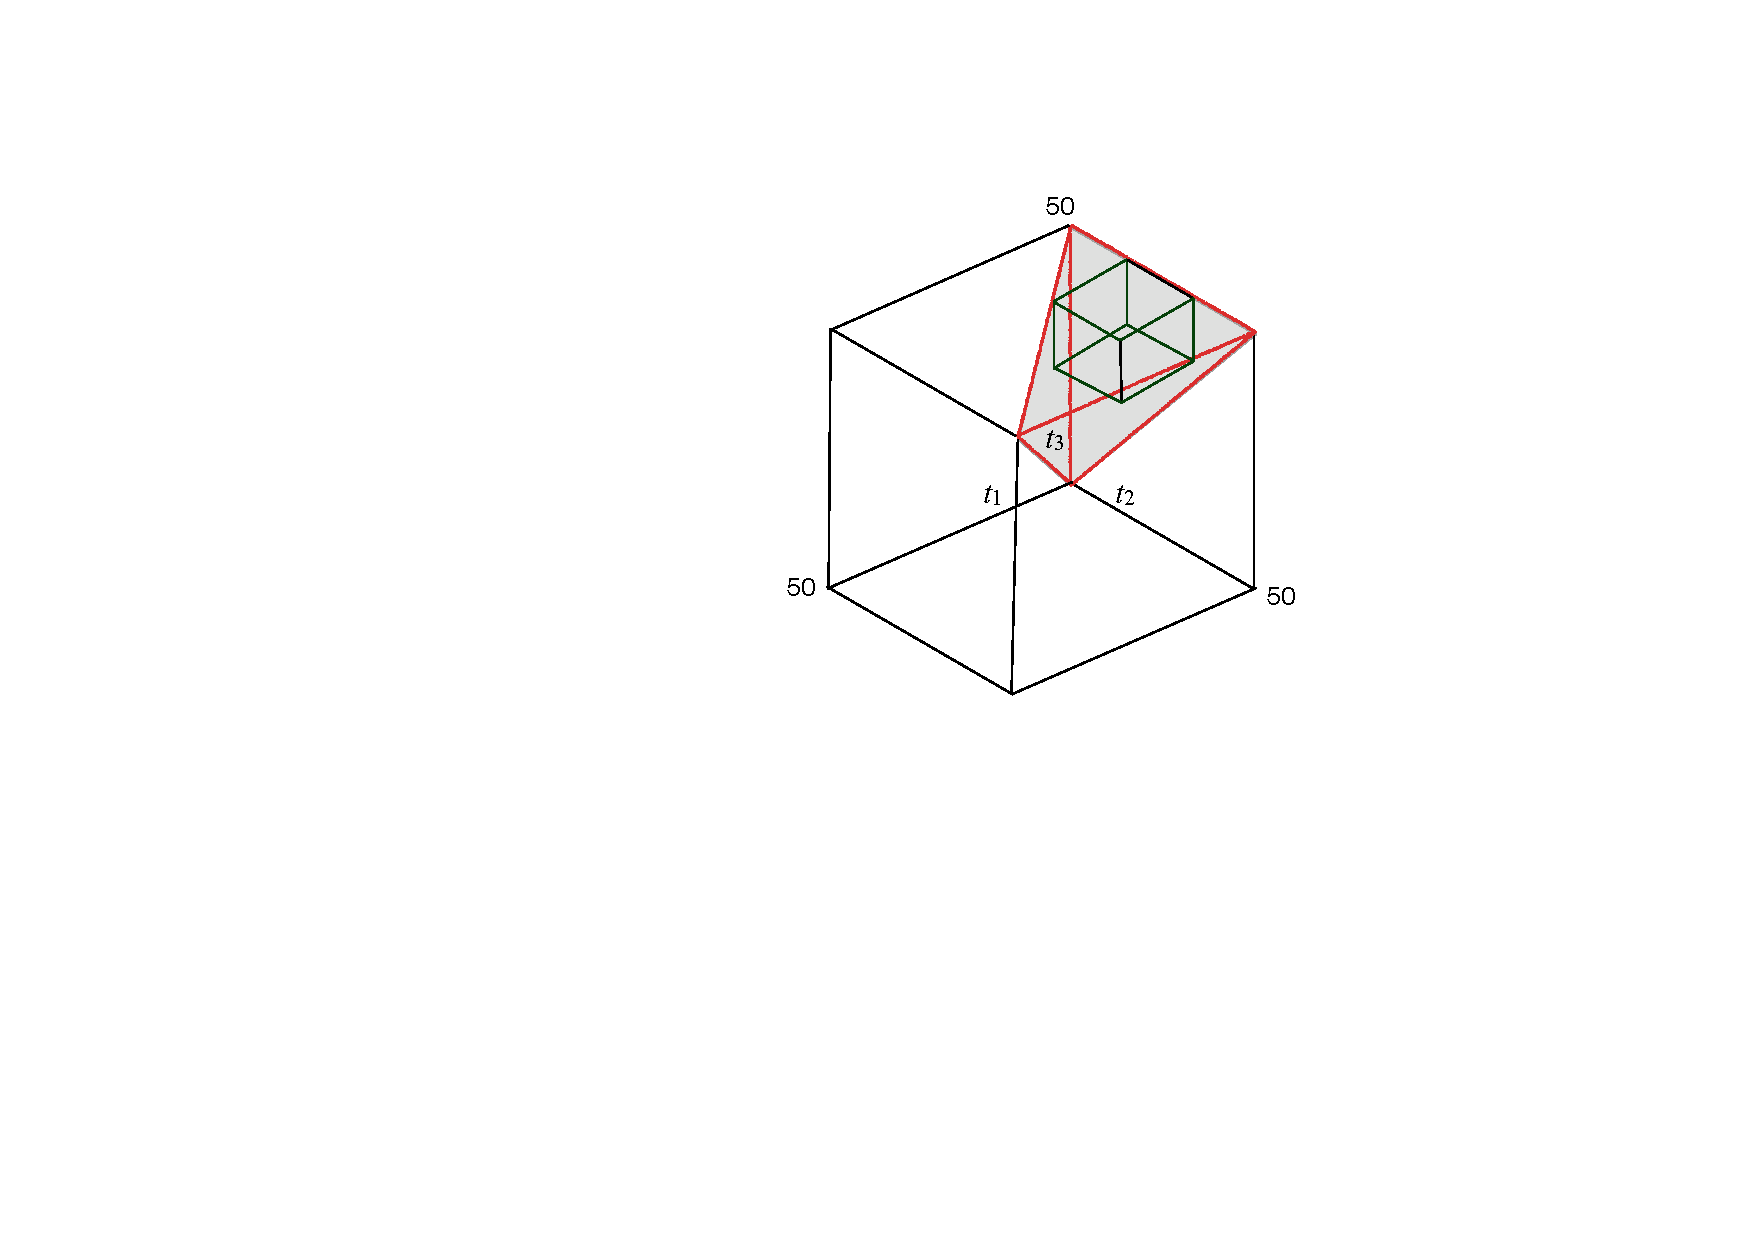
\includegraphics[width=0.3\textwidth]{chapter/icaps-flexibility/polytopes.pdf}
\caption{The polytope $P_1$ generated by $S_1$ is a cube with edges of size 50; the polytope $P_2$ generated by $S_2$ is the shaded subspace of $P_1$. The inner bounding box of $P_2$ is the small green cube in the shaded area. The inner bounding box of $S_1$ and also the outer bounding box of $S_1$ and $S_2$ equal $P_1$.}
\label{Fig1}
\end{figure}
\vspace{-0.8cm}\mbox{}\\
\end{example}
A new flexibility metric for STNs  \cite{wilson:2013} has been introduced to overcome the disadvantages of $\flex(S)$.
Instead of determining the smallest \emph{outer bounding box} (hypercube) containing the polyhedron generated by a set of constraints $C$, they determine the largest \emph{inner bounding box} contained in this polyhedron (see below for a computation).
An obvious advantage of such an inner bounding box is that every point in the box belongs to the polyhedron (i.e.\ solution space) containing it.
\begin{example}
Consider again the STN $S_2$. A largest inner bounding box contained in the polytope determined by $C_2$ is the small box contained in the shaded area in Figure~\ref{Fig1}. All its points are contained in the solution space of $S_2$.
\end{example} 
To construct a flexibility metric based on the largest inner bounding box we have to make sure that for every constraint $t_j - t_i \leq c_{i,j}$  the flexibility intervals  $[t^-_i, t^+_i]$ and $[t^-_j, t^+_j]$ associated with $t_i$ and $t_j$ are independent, i.e., every value $v_i$ and $v_j$ for $t_i$ and $t_j$, respectively, chosen in these intervals has to satisfy the constraint $v_j - v_i \leq c_{i,j}$. 
This is exactly the case if $t_j$ assumes the maximum value and $t_i$ assumes the minimum value in its interval, i.e., we have to ensure that $t^+_j - t^-_i \leq c_{i,j}$.
Therefore, the value $\flex^*(S)$ for the concurrent flexibility for $S$ can be found by solving the following LP (see \cite{wilson:2014}):
%The key idea in using the largest inner bounding box is that a flexibility metric based on it ensures that all dependencies between the flexibility intervals $[t^-_i, t^+_i]$ have been removed.
%In order to guarantee complete independence between these intervals, we have to make sure that the upper bounds and lower bounds of these intervals satisfy the constraints imposed on them.
%For example, consider aBut that is the case exactly if $t_j$ is maximal and $t_i$ is minimal, i.e., we have to ensure that $t^+_j - t^-_i \leq c_{i,j}$.
%As we have developed our arguments in detail elsewhere~\cite{wilson:2014-aij}, in this paper we will only give the solution we propose. It consists of assigning an interval to each variable from which \emph{every} value can be chosen, \emph{independently} from the values chosen for other variables. We call such an assignment an \emph{interval schedule}. An STN's flexibility, denoted by $\flex(S)$, will measure the sum of the lengths of these intervals.
%
%\begin{definition}[Interval schedule]
%Given an STN $S=(T,P)$, a set $I_S=\{I_t=[\ell_t,u_t]\mid t\in T\}$ of non-empty intervals for the time point variables $t\in T$ is an \emph{interval schedule} for $S$ iff for every $t\in T$ and every $v_t\in[\ell_t,u_t]$, the assignment $\sigma$ defined by $\sigma(t)=v_t$ is a schedule for $S$.
%\end{definition}
%
%To compute an interval schedule, we transform the STN $S$ to an STN $S'$ in which new variables $t^-_i$ and $t^+_i$ occur for every $t_i\in T$. These variables model the lower and upper boundaries of the interval assigned to variable $t_i$.
%In order to ensure that the variables $t^-_i$ and $t^+_i$ correspond to their intended meaning, we need to make sure that for every constraint $t_j - t_i\leq c_{i,j}$ in $P$, the intervals assigned to these events should be constrained so that, within their respective intervals, the events can not be scheduled so far apart as to violate the constraint.
%
%\begin{proposition}\label{prop:independent}
%Let $S = (T,P)$ be an STN. A set $I_S = \{ [\ell_{t}, u_{t}]\mid t \in T\}$ of intervals for the variables in $T$ is an interval schedule for $S$, iff for every pair $(t_i, t_j) \in T^2$, %niet T \cup \{z\}, want z zit al in T
%it holds that if $t_j - t_i \leq c_{ij} \in P$, then $u_{t_j} - \ell_{t_i} \leq c_{ij}$.
%\end{proposition}
%\begin{proof}
%(If) Suppose the implication holds for every pair of variables. We have to show that $I_S$ is an interval schedule. So, for every $t \in T$, choose an arbitrary value $v_t \in [ \ell_{t}, u_{t}]$ and let $\sigma$ be defined by $\sigma(t)=v_t$, for all $t\in T$. We must show that $\sigma$ is a schedule for $S$. Suppose $\sigma$ is not a schedule, but that it violates some constraint in $P$, say $t_j - t_i \leq c_{ij}$. Observe that we have assumed that the fact that this constraint is an element of $P$, implies that $u_{t_j} - \ell_{t_i} \leq c_{ij}$. The fact that this constraint is violated by $\sigma$ means that $\sigma(t_j) - \sigma(t_i) > c_{ij}$. But this implies that $c_{ij} < v_{t_j} - v_{t_i} \leq u_{t_j} - \ell_{t_i}$, since $v_{t_j}\leq u_{t_j}$ and $v_{t_i}\geq\ell_{t_i}$. Thus $u_{t_j} - \ell_{t_i}>c_{ij}$, which contradicts the fact that $u_{t_j} - \ell_{t_j} \leq c_{ij}$, so $\sigma$ is a schedule for $S$.
%
%(Only if) Suppose the set $I_S$ is an interval schedule for $S$. Take an arbitrary pair $(t_i,t_j)\in T^2$, and suppose $t_j-t_i\leq c_{ij}\in P$. Because $I_S$ is an interval schedule, there is a schedule $\sigma$ for $S$ such that $\sigma(t_j)=u_{t_j}$ and $\sigma(t_i)=\ell_{t_i}$. Because $\sigma$ is indeed a schedule, it satisfies all constraints in $P$, so we know that $u_{t_j}-\ell_{t_i}\leq c_{ij}$. 
%\end{proof}
%
%This result tells us which constraints the endpoints of an interval schedule have to satisfy. We will therefore view the interval \emph{endpoints as variables}, and compute values for them when they are subjected to these constraints. In particular, from the STN $S$ we compute interval endpoints as the solution of a derived STN $S'=(T',P')$, which has two interval end points $t_i^-$ and $t_i^+$ for every $t_i\in T$. We have just seen intuitively how we should fill the set of constraints $P'$. More precisely, to $P'$ we add a constraint $t_j^+-t_i^-\leq c_{ij}$  for every constraint $t_j-t_i\leq c_{ij}$ in $P$, and a constraint $t_i^--t_i^+\leq 0$ for every $t_i\in T$.
%
%\begin{proposition}
%Let $S =(T,P)$ be an STN. Consider the STN  $S' = (T', P')$ where
%\begin{align*}
%T' = &\ \{ t^+, t^- \mid t \in T \} \cup \{z'\}, \\
%P' = &\ \{ t^+ - t'^- \leq c \mid t - t' \leq c \in C \}\ \cup \\
%&\ \{ t^- -t^+ \leq 0 \mid t\in T \}\ \cup\\
%&\ \{ z' - t_0^- \leq 0, t_0^+-z'\leq0\}.
%\end{align*}
%Then, for every solution $\sigma'$ of $S'$, the set $\{ [\sigma'(t^-), \sigma'(t^+)] \mid t \in T \}$ is an interval schedule for $S$.
%\end{proposition}
%\begin{proof}
%First we establish that there actually exists a solution $\sigma'$ for $S'$. We have assumed that $S$ is consistent, so there exists a schedule $\sigma$ for $S$. Take such a schedule, and construct an assignment $\sigma'$ for $S'$ as follows: For every $t\in T$, let $\sigma'(t^+)=\sigma'(t^-)=\sigma(t)$. It can readily be verified from the construction of the set $P'$ that $\sigma'$ satisfies all those constraints.
%
%So we can now take an arbitrary schedule $\sigma'$ for $S'$ and show that the set $\{[\sigma'(t^-),\sigma'(t^+)]\mid t\in T\}$ is an interval schedule for $S$. Take an arbitrary constraint $t_j-t_i\leq c_{ij}\in P$. By Proposition~\ref{prop:independent} it suffices to show that $\sigma'(t_j^+)-\sigma(t_i^-)\leq c_{ij}$. Because the constraint $t_j-t_i\leq c_{ij}\in P$, the constraint $t^+_j-t^-_i \leq c_{ij}$ was added in the construction of $P'$, and since $\sigma'$ is a schedule for $S'$, it satisfies this constraint.
%\end{proof}
%
%Although our transformation of $S$ into $S'$ provides us with an interval schedule for $S$, we have yet to determine the flexibility of $S$, since the sum of the sizes of these intervals does not need to be maximal.
%To obtain the flexibility  measure, we have to select a solution $\sigma'$ for $S'$ that maximizes the sum of the sizes of the intervals.
%%To take into account these dependencies, for every $t_i \in T$  respectively. For every $t_i$ we also define a function $f_i$ that returns the interval (flexibility) $(t^-_i, t^+_i)$ for $t_i$ \emph{given} the corresponding intervals (flexibilities) $(t^-_j, t^+_j)$ for all other events $t_j \neq t_i$. In general,
%%\[
%%f_i((t^-_1, t^+_1), \ldots (t^-_{i-1}, t^+_{i-1}), (t^-_{i+1}, t^+_{i+1}), \ldots, (t^-_{n}, t^+_{n})) = (t^-_i, t^+) \]
%%
%%This function $f_i$ is specified such that 
%%\begin{enumerate}
%%\item every starting time $v \in (t^-_i, t^+)$ can be chosen for $t_i$, whatever starting times in the intervals  $(t^-_j, t^+_j)$ are chosen for the other events, 
%%\item the size $t^+_i - t^-_i$ of the interval $[ t^-_i , t^+_i ]$ is maximal.
%%\end{enumerate}
%%In other words, the flexibility $flex(t_i) = (t^+_i - t^-_i)$ is a real flexibility assigned to event $t_i$ and is independent of the flexibilities $flex(t_j) = (t^+_j - t^-_j)$ assigned to other events.
%%Since we would like to maximise the sum $\Sigma^n_{i=1} flex(t_i)$ as a metric for the real flexibility of $S$, we define $flex(S)$ as follows:
%%\begin{equation}\label{flex.1}
%% flex(S) = max_{t^-_1, t^+_1, \ldots t^-_n, t^+_n}\Sigma^n_{i=1} (t^+_i - t^-_i)
%%\end{equation}
%%where
%%\[ f_i((t^-_1, t^+_1), \ldots (t^-_{i-1}, t^+_{i-1}), (t^-_{i+1}, t^+_{i+1}), \ldots, (t^-_{n}, t^+_{n})) = (t^-_i, t^+_i) \]
%%
%%The problem to find a suitable flexibility metric now has been reduced to finding suitable functions $f_i$ satisfying the requirements mentioned.
%%Fortunately, due to the fact that possible correlations between events are specified through linear constraints in an STN, we can easily 
%%find suitable specifications for such functions $f_i$:
%%\begin{proposition}
%%Let $S = (T, C)$ be an STN. If, for $j =1, \ldots, i-1, i+1, \ldots n$ the intervals $(t^-_j, t^+_j)$ are given, the function 
%%
%%$f_i((t^-_1, t^+_1), \ldots (t^-_{i-1}, t^+_{i-1}), (t^-_{i+1}, t^+_{i+1}), \ldots, (t^-_{n}, t^+_{n})) = (t^-_i, t^+_i)$
%%
%%\noindent 
%%can be specified as follows:
%%\begin{enumerate}
%%\item
%%$t^+_i$ is the maximal value of the variable $t_i$ satisfying all constraints $t_i - t^-_j \leq c_{ij} \in C$ as well as the constraint $t_i -z \leq c_i \in C$;
%%\item
%%$t^-_i$ is the minimal value of the variable $t_i$ satisfying all constraints $t^+_j - t_i \leq c_{ij} \in C$ as well as the constraint $z -t_i \leq c'_i \in C$.
%%\end{enumerate}
%%\end{proposition}
%%
%%\begin{proof}
%%\end{proof}
%We then need the following LP to find the maximizer that will guarantee a set of maximal and independent flexibilities:

%\begin{theorem}\label{thm:maxFlex}
%Let $S = (T, P)$ be an STN. Then $\flex(S)$ can be computed by solving the following linear program:
%\marginpar{We need to motivate $t^- \leq t^+$ here and to show that this condition does not affect the optimum }
\begin{alignat*}{2}\label{LP1} \tag{LP1}
\text{maximize}                      &\quad \sum_{t_i \in T}{(t^+_i - t^-_i)}  \\
\text{subject to }  &\quad  t^-_i                         \leq t^+_i  &, & \quad \forall\; t_i\in T  \\  
                            &\quad  t^+_j - t^-_i                 \leq  c_{i,j}   &, & \quad \forall\;( t_j  - t_i  \leq c_{i,j}) \in C
\end{alignat*}
%\end{theorem} 

%As a consequence, we have the following corollary.
%\begin{corollary} \label{obs.1}
%Given an STN $S = (T,P)$,  the  flexibility metric $\flex$ determines an assignment $\flex(t) = [t^-, t^+]$, such that for every $t \in T$ and every $v_t \in [t^-, t^+]$, the assignment $\sigma(t) = v_t$ is a fixed-time schedule for $S$ (and thus satisfies all constraints in $C$).
%\end{corollary}

%\begin{example}
%%\marginpar{(Text needs to adapted)}
%If we apply this method to the example from the previous section, we find that for this STN $S$, $\flex(S)=7$, which is attained by the following interval schedule:
%\begin{align*}
%\sigma'(z^-)&=0 &\sigma'(z^+)&=0 \\
%\sigma'(e_1^-)&=0&\sigma'(e_1^+)&=1\\
%\sigma'(e_2^-)&=5&\sigma'(e_2^+)&=5\\
%\sigma'(c_1^-)&=2&\sigma'(c_1^+)&=3\\
%\sigma'(c_2^-)&=5&\sigma'(c_2^+)&=5\\
%\sigma'(b^-)&=5&\sigma'(b^+)&=10\\
%\end{align*}
%We see that the flexibility that can be attained is much lower than as computed by the other methods mentioned earlier. Of course, other schedules are possible as well, for example, where all bounds are shifted in time. %All flexibility-maximizing interval schedules have in common that one unit of flexibility is divided among the two variables $e_1$ and $e_2$, and that this is also the case for the two variables $c_1$ and $c_2$, and that five units of flexibility is assigned to the event $b$.
%\end{example}
Here, $\flex^*(S)$ indicates the maximum flexibility that can be obtained when all flexibility intervals of temporal variables are independent from each other and values in these intervals can be chosen concurrently.
\begin{example}
 \emph{\ref{LP1}} will return $\flex^*(S_1) = 150$, but $\flex^*(S_2) = 50$, showing that here the concurrent flexibility metric corresponds to our intuition.
\end{example}

\section{Concurrent flexibility by minimum matching}
In this section we show that computing the maximum concurrent flexibility is identical to computing a perfect minimum weight matching of a weighted bipartite graph $G_S$ completely specified by $D_S$. On the other hand, computing the naive flexibility corresponds to computing a maximum matching in this graph $G_S$.

To establish these results, first, we specify an LP equivalent to \ref{LP1} using the minimum distance matrix $D_S$ instead of the original set $C$ of constraints. 
Then we show that the entries of $D_S$ can be used to compute a least upper bound on $\flex^*(S)$.
Finally, by using duality theory in Linear Programming and some adaptations, we show that this least upper bound is a maximum matching in a bipartite graph specified by $D_S$ and in fact equals $\flex^*(S)$.
 
Remember that the entries $d(i,j)$ of the minimum distance matrix $D_S$ of an STN $S$ specify the upper bound of the strongest difference constraint between the temporal variables $t_j$ and $t_i$:
$t_j - t_i \leq d(i,j)$. 
%Referring to the derivation of $\flex^*(S)$ we note that in using these strongest constraints, $t_j - t_i \leq d(i,j)$ implies that $t^+_j - t^-_i \leq d(i,j)$.
Hence, we can replace the specification \ref{LP1} by the following equivalent LP, since both LP's specify the same solution space:
\begin{alignat*}{2}\label{LP2} \tag{LP2}
\text{maximize}                       &\quad \sum_{t_i \in T}{(t^+_i - t^-_i)}  \\
\text{subject to }  &\quad t^-_i                       \leq t^+_i  &\quad , &\quad \forall\; t_i \in T \notag \\
                           &\quad t^+_j - t^-_i                  \leq  d(i,j)  &\quad , &\quad \forall\; t_i \neq t_j \in T \notag
\end{alignat*}

To remove the condition $\forall\; t_i \neq t_j \in T$, it is sufficient to realize that $
t^+_i - t^-_i = (t^+_i - t^-_0) + (t^+_0 - t^-_i) 
                    \leq d(0,i)+d(i,0) = \lst(t_i) -  \est(t_i)$,
since $t^-_0 = t^+_0 = 0$.
Hence, setting $ d(i,i) = d(0,i)+d(i,0)$ for all $t_i \in T$, we change \ref{LP2} to the following equivalent LP:
\begin{alignat*}{2}\label{LP4} \tag{LP3}
\text{maximize}                       & \sum_{t_i \in T}{(t^+_i - t^-_i)} & \\
\text{subject to }  &  t^-_i                        \leq t^+_i &\quad, \quad & \forall\; t_i \in T \notag \\
                            & t^+_j - t^-_i                  \leq  d(i,j)  &\quad, \quad  & \forall\; t_i, t_j \in T \notag
\end{alignat*}

We will denote this modified distance matrix $D_S$, where $d(i,i) = \lst(t_i)-\est(t_i)$, by $D^*_S$.

Now consider the sum
$\sum^n_{i=1} (t^{+}_i - t^-_i) $
we want to maximize.
%The concurrent flexibility $\flex^*$ is computed as the maximum of this sum under the constraints as given in \ref{eq.?}.
This sum can be rewritten as
$\sum^n_{i=1} (t^{+}_i - t^-_i)  = \sum^n_{i=1} (t^+_i - t^-_{\pi(i)})
$
for an arbitrary permutation $\pi$ of $(1,2, \ldots, n)$.
Since $t^+_i -  t^-_{\pi(i)} \leq d(\pi(i),i)$, we can derive an upper bound on this sum for every permutation $\pi$:
$  \sum^n_{i=1} (t^+_i - t^-_{\pi(i)}) \leq \sum^n_{i=1} d(\pi(i),i)$.
In particular, there are permutations $\pi^*$ such that for all permutations $\pi$ it holds that
$  \sum^n_{i=1} d(\pi^*(i),i) \leq \sum^n_{i=1} d(\pi(i),i) $.
Such a (smallest) permutation $\pi^*$ specifies a least upper bound on $\flex^*(S) = \max  \sum^n_{i=1} (t^{+}_i - t^-_i)$.

There is an efficient  way to compute such a smallest permutation $\pi^*$ by obtaining a \emph{minimum weighted matching} between $T^+ = \{t^+_1, t^+_2, \ldots, t^+_n\}$ and $T^- = \{t^-_1, t^-_2, \ldots, t^-_n\}$:
Consider the weighted complete graph $G_S = (V, E, w)$ where $V = T^+ \cup T^-$, the edges $\{t^+_i, t^-_j \} \in E$ for $i, j =1,\dots n$, and for every edge $\{t^+_i, t^-_j\}$ its weight $w_{i,j} = d_{j,i}$. Note that $G_S$ is completely specified by $D^*_S$.
By Hall's theorem, this graph has a minimum weighted perfect matching, that is a set $M \subseteq E$ of $n$ edges covering $T^+$ and $T^-$ such that the sum of these edges is minimum.
Clearly,  such a minimum weighted matching determines a permutation $\pi^*$ such that  $\sum^n_{i=1} d(\pi^*(i),i)$ is minimum.
Since it holds that $ \sum_{t_i \in T}(t^+_i - t^-_i) \leq \sum^n_{i=1} d(\pi^*(i),i)$,
the cost $c(M)$ of such a minimum matching provides an upper bound for $\flex^*(S)$.

Actually, by applying simple LP-duality theory, we can do  better and show that there exists an \emph{exact} correspondence between a minimum matching in $D^*_S$ and the maximum concurrent flexibility $\flex^*(S)$:

\begin{proposition}
Let $S = (T,C)$ be a consistent STN having a minimum distance matrix $D_S$. Then the concurrent flexibility $\flex^*(S)$ of $S$ equals the cost $c(M)$ of a minimum matching $M$ of the complete weighted graph $G_S$ specified by $D^*_S$.
\end{proposition}
\begin{proof}
The most elegant way to prove this result is making use of duality in linear programming.
The dual of \ref{LP4} is the following LP:
\begin{alignat*}{2}
\label{LP5} 
\tag{LP4}
\text{minimize}                       &\quad \sum_{1 \leq i,j \leq n} d(i,j) \, y_{j,i} \\
\text{subject to }  &\quad  \sum^n_{j=1} y_{i,j} = 1  + y_{0,i} \quad                &, &\; i \in \{1,2,\ldots n\} \notag \\
                           &\quad  \sum^n_{i=1} y_{i,j}               = 1  + y_{0,j} \quad &, &\; j \in \{1,2,\ldots n\} \notag \\
                           &\quad  y_{i,j} \geq 0 \quad & , &\; i,j \in \{0,1,\ldots, n \} \notag
\end{alignat*}
Since the original LP (\ref{LP4}) has an optimal solution, by strong duality, the objective values of optimal solutions of both LP's coincide. 
The constraint matrix associated with both LP's is total unimodular, hence, \ref{LP5} has integral optimal solutions.
This dual \ref{LP5} can be interpreted as follows: 
%assume all $y_{0,i} = 0$ for all $i=1,2, \ldots n$ and 
Let $G_S$ be a complete bipartite graph having two sets of nodes  $A = \{1, \ldots, n \}$ and $B = \{1, \ldots n \}$, representing the rows and columns of $D^*_S$. Let $D^*_S$ specify the weights $d(j,i)$ of the edges $e=(i,j)$ of $G_S$.
Then, in case $y_{0,i} = 0$ for all $i=1,2, \ldots n$), it is not difficult to see that a minimizer for \ref{LP5} specifies a minimum weight matching $M$ in $G_S$.
By strong duality, the cost $c(M)$ of $M$ corresponds to  $\flex^*(S)$.
 
Therefore, the only part left to prove is to show that the assumption $y_{0,i} = 0$ for all $i=1,2, \ldots n$ does not affect the \emph{value} of the solutions to \ref{LP5}:\\[1ex]
\noindent {\bf Claim } Whenever \ref{LP5} has an optimal integral solution, there also exists an integral solution of \ref{LP5} with at most the same cost such that $y_{0,i}=0$,  for all $i=1,2, \ldots, n$.\\[1ex]
\noindent {\bf Proof of the Claim } Suppose there exists an integral solution ${\b y^*}= (y^*_{i,j})$ for  \ref{LP5} where $ y^*_{0,i} > 0$ for some $1 \leq i \leq n $.  
Then there exist  $j, k \in \{1, \ldots, n\}$, $j \neq i$ and $k \neq i$, such that $y^*_{i,j} = 1$ and $y^*_{k,i} =1$.\footnote{Wlog.\ we may assume $y^*_{i,j} \in \{0,1\}$, $1 \leq i,j \leq n$: If $y^*_{i,j}>1$ then there exists a solution ${\bf y'}$ with $c({\bf y'}) \leq c({\bf y}^*)$ s.t.\  $y'_{i,j}=1$ and  $y'_{0,i} =  y^*_{0,i} - (y^*_{i,j} - 1)$.}
This condition violates the matching conditions.
But then, since $ d(j,k) \leq d(j,i) + d(i,k)$, there exists a solution ${\bf y} = (y_{i,j})$ such that $c({\bf y}) \leq c({\bf y}^*)$ where $y_{i,j} =y_{k,i} = 0$ and $y_{k,j} = 1$, and 
 $y_{0,i} = y^*_{0,i} - 2 + y^*_{k,j}$. Hence,  there exists a solution $\bf y$ with at most the same cost as ${\bf y^*}$ such that $0 \leq y_{0,i} < y^*_{0,i}$.
%$  \sum^n_{j=1} y_{j,i}               = 1  + y'_{0,i} $
%and 
%$\sum^n_{j=1} y_{i,j}              = 1  + y'_{0,i}$ 
%and $0 \leq y'_{0,i} < y_{0,i}$. 
Iterating this procedure, we conclude that there exists a solution such that $y_{0,i} = 0$ as well, with cost not exceeding the cost of the original solution.
This procedure can be repeated until we have obtained an optimal solution where it holds that $y_{0,i} = 0$ for all $i$, i.e., a perfect minimum weight matching, thereby proving the claim.
\end{proof}
A maximum matching $M$ for  $D^*_S$ can be determined immediately:
Note that the value of any matching $M'$ realised by a permutation $\pi'$ satisfies 
%\begin{align*}
%  \sum^n_{i=1} d(i, \pi'(i)) & \leq \sum^n_{i=1} d(i,0) + d(0,\pi'(i)) \\
%   & = \sum^n_{i=1} d(i,0) + d(0,i) \\
%   & = \sum^n_{i=1} \lst(t_i) - \est(t_i) = \flex(S)
%\end{align*}
 $ \sum^n_{i=1} d(i, \pi'(i))  \leq \sum^n_{i=1} d(i,0) + d(0,\pi'(i)) 
    = \sum^n_{i=1} d(i,0) + d(0,i) 
    = \sum^n_{i=1} \lst(t_i) - \est(t_i) = \flex(S).
$
Since $d(i,i) = \lst(t_i) - \est(t_i)$, the matching $M = \{ (i, i) : i=1,2, \ldots, n \}$ realized by  $\pi(i)=i$, is a maximum matching for $D^*_S$:
\begin{proposition}
Let $S = (T,C)$ be a consistent STN having a minimum distance matrix $D_S$. Then the \emph{naive flexibility} $\flex(S)$ of $S$ equals the cost $c(M)$ of a \emph{maximum matching} $M$ of the weighted graph specified by $D^*_S$.
\end{proposition}

%\begin{example}[from~\cite{planken:2013}]\label{example:information}
%To illustrate the results we have obtained, we discuss a slightly larger example. 
%Let us face the problem of having breakfast. Our breakfast requires some preparation: we want to make coffee and boil eggs. Both of these activities are represented by their start and end time points: $e_1$ and $e_2$ for the task of boiling the eggs, which takes between 4 and 5 minutes, and $c_1$ and $c_2$ for making coffee, which requires 2 to 3 minutes. We start preparing our meal at 9 AM, marked by the temporal reference point $z$, and $b$ takes the role of horizon, denoting the moment when both coffee and eggs are done and we sit down to enjoy breakfast. We do not want our coffee or eggs to get cold, so we constrain the duration of time from $e_2$ and $c_2$ to $b$ to at most 8 and 5 minutes, respectively. Since everybody is a little hungry, we want to be done [with the preparations] within 15 minutes.
%Figure~\ref{fig:example:STN}
%\begin{figure}[ht]\centering
%%\subfloat[STN\label{fig:example:STN}]
%{
%\begin{tikzpicture}%[xscale=0.7,yscale=0.8]
%	\begin{scope}
%		[every node/.style={draw,circle}]
%		\path (0,2) node (z) {$z$}
%		(2,0) node (c1) {$c_1$}
%		(2,4) node (e1) {$e_1$}
%		(4,0) node (c2) {$c_2$}
%		(4,4) node (e2) {$e_2$}
%		(6,2) node (b) {$b$};
%	\end{scope}
%
%	\begin{scope}[every path/.style={-latex}]
%		\draw (z) -- node[above left] {$[0,\infty)$} (e1);
%		\draw (z) -- node[below left] {$[0,\infty)$} (c1);
%		\draw (z) -- node[above] {$[-\infty,15]$} (b);
%		\draw (e1) -- node[above] {$[4,5]$} (e2);
%		\draw (c1) -- node[above] {$[2,3]$} (c2);
%        \draw (e2) -- node[above right] {$[0,8]$} (b);
%        \draw (c2) -- node[below right] {$[0,5]$} (b);
%    \end{scope}
%\end{tikzpicture}
%}
%%}\hfill
%%\subfloat[Distance graph\label{fig:example:distance}]{
%%\begin{tikzpicture}%[xscale=0.8,yscale=0.8]
%%	\begin{scope}
%%		[every node/.style={draw,circle}]
%%		\path (0,2) node (z) {$z$}
%%		(2,0) node (c1) {$c_1$}
%%		(2,4) node (e1) {$e_1$}
%%		(4,0) node (c2) {$c_2$}
%%		(4,4) node (e2) {$e_2$}
%%		(6,2) node (b) {$b$};
%%	\end{scope}
%%
%%	\begin{scope}[every path/.style={-latex}]
%%		\draw (e1) -- node[above left] {$0$} (z);
%%        \draw (e1) to[out=330,in=210] node[above] {$5$} (e2);
%%        \draw (e2) to[out=150,in=30] node[above] {$-4$} (e1);
%%		\draw (c1) -- node[below left] {$0$} (z);
%%		\draw (z) -- node[above] {$15$} (b);
%%        \draw (c1) to[out=330,in=210] node[above] {$3$} (c2);
%%        \draw (c2) to[out=150,in=30] node[above] {$-2$} (c1);
%%        \draw (e2) to[out=345,in=105] node[right] {$8$} (b);
%%        \draw (b) to[out=165,in=285] node[left] {$0$} (e2);
%%        \draw (c2) to[out=15,in=255] node[right] {$5$} (b);
%%        \draw (b) to[out=195,in=75] node[left] {$0$} (c2);
%%    \end{scope}
%%\end{tikzpicture}
%%}
%\caption{The STN encoding of example~\ref{example:information}.}
%\label{fig:example}
%\end{figure}
%shows an encoding as an STN of the information in example~\ref{example:information}.
%Computing the naive flexibility $\flex(S)$ results in $\flex(S) = 0+11+13+11+13+11 = 59$ while using the LP approach we
%obtain $\flex^*(S) = 7$.
%Using the correspondence with matching,  
%we use the following  modified minimum distance matrix $D^*_S$:
%%\begin{equation*}
%%\begin{matrix}
%%D_S = \left[\begin{array}{rrrrrr}
%%                  0 & 11  & 13 & 15 & 15 & 15\\
%%                  0 & 0 & 11 & 5 & 13 & 13   \\
%%                  0 & 4  & 0  & 8 & 3 & 8 \\
%%                  -4 & -4 & 6 & 0 & 8 & 8 \\
%%                  -2 & 1 & -2 & 5 & 0 & 5 \\
%%                  -4 & -4 & -2 & 0 & 0 & 0  
%%                   \end{array} \right]
%%\end{matrix}
%%\end{equation*}
%%%We consider the distance matrix as the specification of a bipartite graph $G_S$ connecting nodes $t^+_i \in T^+$  and $t^-_i \in T^-$. To use this matrix for computing a minimum matching, we have to adapt it slightly. First of all, while the cost of connecting $t^-_0$ and $t^+_0$ is 0,  the cost of connecting $t^-_i$ and $t^+_i$ should be high enough to prevent the edges $(t^-_i, t^+_i)$ to occur in any minimum matching. We therefore set them to $d = \max{d(i,j)} + 1$.
%%The adapted matrix $D^*_S$ then equals
%\begin{equation*}
%\begin{matrix}
%D^*_S = \left[\begin{array}{rrrrrr}
%                  \bf{0} & 11  & 13 & 15 & 15 & 15\\
%                  0 & 11 & 11 & \bf{5} & 13 & 13   \\
%                  0 & 4  & 13  & 8 & \bf{3} & 8 \\
%                  -4 & \bf{-4} & 6 & 11 & 8 & 8 \\
%                  -2 & 1 & -2 & 5 & 13 & \bf{5} \\
%                  -4 & -4 & \bf{-2} & 0 & 0 & 11  
%                   \end{array} \right]
%\end{matrix}
%\end{equation*}
%A minimum matching $M$ obtained by applying e.g. the hungarian method, results in \[ M = \{ (0, 0), (1, 3), (2, 5), (3, 1), (4, 2), (5, 4) \} \]
% and the associated cost $C(M)$ are equal to 
% \[c(M) = -4 + -2 + 5 + 3 + 5 = 7.\] Hence $\flex^*(S)= 7$, as we already observed.
%\end{example}

\section{From $O(n^5)$ to $O(n^3)$ to compute  flexibility}

The complexity of computing the concurrent flexibility of an $STN$ by an LP method depends on the exact method used for the LP solver. Currently, the best (interior-point based) LP-solvers have a complexity of $O(n^3 L)$ \cite{potra2000} where $n$ is the number of unknowns to solve for (the dimension of the vector $x$) and $L$ is the input complexity, i.e., the bit length of the input description. This means that given an STN $S = (T, C)$, the currently best LP-solvers could need $O(n^3 m)$-time to find the concurrent flexibility $\flex^*(S)$, where $n = |T|$ and $m = |C|$. Since $m = O(n^2)$, we could expect a worst-case running time $O(n^5)$ to compute $\flex^*(S)$.

The correspondence (flexibility $\equiv$ matching) obtained in the previous section allows us to present a better upper bound of the running time needed to compute the maximum concurrent flexibility.
For, we know that given an STN $S$ its minimal distance matrix $D_S$ can be computed in $O(n^3)$ time. A minimum matching algorithm based on the specification of $D_S$ also requires $O(n^2 \log{n} + n \times n^2) = O(n^3)$-time \cite{Fredman:1987}. Hence, the total computation time for determining a minimum matching is $O(n^3)$-time. 
Note that computing the naive flexibility also requires an $O(n^3)$ computation of earliest and latest times for the temporal variables, both of which can be obtained via $D_S$.

Hence, in conclusion, we obtain the following result:

\begin{proposition}
The concurrent flexibility as well as the naive flexibility of an STN $S$ can be computed in $O(n^3)$-time.
\end{proposition}

\section{Conclusion}
We established a connection between the computation of two flexibility metrics and properties of the minimal distance matrix $D_S$ of an STN $S$: computing the concurrent flexibility metric is identical to computing a minimum weight matching of a weighted bipartite graph completely specified by the minimum distance matrix $D_S$. On the other hand, computing the naive flexibility metric corresponds to computing a maximum matching in this graph.
%Pointing out this correspondence also has a practical advantage: instead of using an LP-based approach to compute the naive flexibility metric whose worst-case complexity is bounded by $O(n^5)$, we are able to derive an $O(n^3)$ algorithm for computing the concurrent flexibility.


%\newpage
%\bibliographystyle{aaai}
%\bibliography{Flexibility}  % name your BibTeX data base
%\end{document}
%


\chapter[Dynamic temporal decoupling]{Dynamic temporal decoupling\protect\footnotemark{}\protect\footnotetext{
This chapter has been published as:
K.S. Mountakis, T.B. Klos and C. Witteveen.  Dynamic Temporal Decoupling. 
In \emph{International Conference on AI and OR Techniques in Constraint Programming for Combinatorial Optimization Problems (CPAIOR)}, pages 328-343, 2017.}}
\label{chapter/cpaior-decoupling}

\section{Introduction}
In quite a number of cases a joint task has to be performed by several actors, each controlling only a part of the set of task constraints. 
For example, consider making a joint appointment with a number of people, constructing a building that involves a number of (sub)contractors, 
or finding a suitable multimodal transportation plan involving different transportation companies. 
In all these cases, some task constraints are under the control of just one actor (agent), 
while others require more than one agent setting the right values to the variables to satisfy them. 
Let us call the first type of constraints \emph{intra-agent} constraints and the second type  \emph{inter-agent} constraints.

If there is enough time, solving such multi-actor constraint problems might involve consultation, negotiation or other agreement technologies.
%While there exists quite some literature on this subject and quite ingenious solution strategies have been proposed, 
Sometimes, however, we have to deal with problems where communication between agents during problem solving is not possible
or unwanted. For example, if the agents are in competition, there are legal or privacy issues preventing communication, or there is simply no time for
communication. 

In this chapter we use an approach to solve multi-actor constraint problems in the latter contexts: 
instead of using agreement technologies, we try to avoid them by providing {\em decoupling techniques}. 
% -- CEES
%Intuitively, a decoupling technique decomposes a multi-actor constraint system in such a way that 
%($i$) all inter-agent constraints are removed, 
%($ii$) each of the agents is able to select a solution for its own set of intra-agent constraints such that 
%($iii$) a simple merging of all individual agent solutions obtained always constitutes a solution to the total set of constraints. 
%So, a decoupling guarantees that partial solutions are conflict-free and always can be simply merged to obtain a complete solution of the original system.
% -- SIMON
Intuitively, a decoupling technique modifies a multi-actor constraint system such that 
each of the agents is able to select a solution for its own set of (intra-agent) constraints 
and a simple merging of all individual agent solutions always satisfies the total set of constraints. 
Usually, this is accomplished by tightening intra-agent constraints such that inter-agent constraints are implied. Examples of real-world applications of such decoupling techniques can be found in e.g.\  \cite{brambilla:2010} and \cite{leeuwen:2009}.
% -- CEES
%Quite some research has been spent on finding suitable decoupling techniques (e.g.,\cite{hunsberger:2002a,brambilla:2010,boerkoel:2013}) for Simple Temporal Problems (STPs),
%a constraint formalism where the constraints $C$ are simple binary difference constraints (\cite{dechter:2003}) over temporal variables $T$ and solutions can be found in low polynomial time ($O(n^3) )$. 
% -- SIMON

Quite some research focuses on finding suitable decoupling techniques (e.g., \cite{hunsberger:2002a,brambilla:2010,boerkoel:2013}) for Simple Temporal Problems (STPs) \cite{dechter:2003}.
An STP $S=(T,C)$ is a constraint formalism where a set of temporal variables $T=\{t_0, t_1,\ldots,t_n\}$ 
are subject to binary difference constraints $C$ and solutions can be found in low polynomial ($O(n^3)$) time. 
Since STPs deal with temporal variables, a decoupling technique applied to STPs is called {\emph{temporal decoupling}.
The quality of a temporal decoupling technique depends on the degree to which it tightens intra-agent constraints:
the more it restricts the flexibility of each individual agent in solving their own part of the constraints, the less it is preferred.
Therefore, we need a flexibility metric to evaluate the quality of a temporal decoupling.

%One such a metric is the (temporal)  \emph{flexibility} of a temporal decoupling. 
Originally, flexibility was measured by summing the differences between the highest possible (latest) and 
the lowest possible (earliest) values of all variables in the constraint system after decoupling (\cite{hunsberger:2002a,hunsberger:2002b}). 
This so-called \emph{naive flexibility metric} has been criticized, however, because it does not take into account the dependencies between the variables and, 
in general, seriously overestimates the ``real'' amount of flexibility.
An alternative metric, the \emph{concurrent flexibility metric} has been proposed in \cite{wilson:2014}. 
This metric accounts for dependencies between the variables and is based on the notion of an \emph{interval schedule} for an STP $S$: 
For each variable $t_i \in T$ an interval schedule defines an interval $[l_i, u_i]$,
%such that every combination $v = (v_1, \ldots, v_n)$ of choices $v_i$ of values in such intervals constitutes a solution for $S$. 
such that choosing a value within $[l_i, u_i]$ for each variable $t_i$, always constitutes a solution for $S$.
The sum $\sum^n_{i=1} (u_i - l_i)$ of the widths of these intervals determines the flexibility of $S$. 
The concurrent flexibility of $S$ then is defined as the maximum flexibility we can obtain for an 
interval schedule of $S$ and can be computed in $O(n^3)$ (see \cite{mountakis:2015}).

As shown in \cite{wilson:2014}, the concurrent flexibility metric can also be used to obtain an optimal (i.e.~maximum flexible) temporal decoupling of an STP. 
This decoupling is a \emph{total decoupling}, that is, a decoupling where the $n$ variables are evenly distributed over $n$ independent agents and thus every agent controls exactly one variable. 
It has been shown that this total decoupling is optimal for every partitioning of the set of temporal variables if one considers the concurrent flexibility metric as the flexibility metric to be used. 
In this paper, we concentrate on such (optimal) total decouplings of an STP. 

%Most literature on temporal decoupling has been concentrated on the centralized computation of a decoupling, cf. \cite{hunsberger:2002b,brambilla:2010}. 
%Recently, however, quite elegant distributed approaches to the construction of a temporal decoupling have been proposed \cite{boerkoel:2013,Mogali:2016}.
%As far as we know, however, no studies have been done on the subject of this paper: the \emph{dynamic temporal decoupling} of STPS.
%This idea can be motivated as follows: 
In all existing approaches, a single temporal decoupling is computed in advance and is not changed, 
even if later on some agents announce their commitment to a specific value (or range of values) for a variable they control. 
%-- CEES
%Intuitively, however, such additional information could be useful for other agents, because it could increase the flexibility of variables they are not yet committed to. 
%They can only profit from such a change in flexibility, however, if the current decoupling would be updated. On the other hand, 
%since agents might not accept modifications in the current decoupling that would impose additional restrictions upon them, 
%we have to make sure that a decoupling update will never negatively affect the current flexibility of any agent, 
%neither globally, nor locally, i.e. with respect to commitments they could have been planning for. 
%-- SIMON
Intuitively, however, we can use such additional information for the benefit of all agents, by possibly increasing the flexibility of variables they are not yet committed to. Specifically, when an agent announces a commitment to a sub-range of values within the given interval schedule (that represents the current decoupling), we are interested in updating the decoupling such that the individual flexibility of no agent is affected negatively. 

More precisely, the overall aim of this paper is to show that a decoupling update method with the following nice properties do exist:  first of all, 
it never affects the current flexibility of the agents negatively, and, secondly, it never decreases (and possibly increases) the individual flexibility of the variables not yet committed to.
We will also show that updating a temporal decoupling as the result of a commitment for a single variable can be done in almost linear (amortized) time ($O(n \log n)$), 
which compares favourably with the cost of computing a new optimal temporal decoupling ($O(n^3)$).

{\bf Organisation } In Sect.~\ref{section:prelim} we discuss existing relevant work on STPs and temporal decoupling (TD).
Then, in Sect.~\ref{section:computing}, extending some existing work, we briefly show how a total TD can be computed in $O(n^3)$, using a minimum matching approach. 
In Sect.~\ref{section:adapt}, we first provide an exact approach to update an existing decoupling after commitments to variables have been made. 
%We show that it satisfies the additional requirement as preserving individual flexibility of variables in case values for one or more variables have been assigned. 
We conclude, however, that this adaptation is computationally quite costly. Therefore, in Sect.~\ref{section:heuristic} we offer an alternative, heuristic method, that is capable to adapt a given temporal decoupling in almost linear time per variable commitment.
To show the benefits of adapting the temporal decoupling, in Sect.~\ref{section:experiments} we present the results of some experiments using STP benchmarks sets with the heuristic decoupling update and compare the results with an exact, but computationally more intensive updating method.
%Almost last, but not least, in Section~\ref{extension}, we show how our approach can be extended to non-total decouplings and how the heuristic can be used to obtain a flexible schedule from a given point-schedule. 
We end with stating some conclusions and suggestions for further work. 


\section{Preliminaries} \label{section:prelim}

\subsubsection{Simple Temporal Problems }
A Simple Temporal Problem (STP) (also known as a Simple Temporal Network (STN)) is a pair $S = (T,C)$, 
where $T = \{t_{0},t_{1}, \ldots, t_{n}\}$ is a set of temporal variables (events) and 
$C$ is a finite set of binary difference constraints $t_{j}-t_{i}\leq c_{ij}$, for some real number $c_{ij}$.\footnote{If both $t_{j}-t_{i}\leq c_{ij}$ and $t_{i}-t_{j}\leq c_{ji}$ are specified, we sometimes use the more compact notations $- c_{ji}\leq t_j - t_i \leq c_{ij}$ or $t_j - t_i  \in [-c_{ji},c_{ij}]$.}The problem is to find a solution, that is a sequence $(s_0, s_1,s_2, \ldots, s_n)$ of values such that, if each $t_i \in T$ takes the value $s_i$, all constraints in $C$ are satisfied.
%A solution to $S$ is a \emph{(point) schedule} for $S$, that is, a function $\sigma: T \rightarrow \mathbb{R}$, assigning a real value (time-point) to each temporal variable in $T$, such that all constraints in $C$ are satisfied. 
If such a solution exists, we say that the STN is \emph{consistent}. \footnote{W.l.g., in the remainder of the paper we simply assume an STN to be consistent. Consistency of an STN can be determined in low-order polynomial time~\cite{dechter1991}.}
In order to express absolute time constraints, the time point variable $t_{0} \in T$, also denoted by $z$, is used. It represents a fixed reference point on the timeline, and is always assigned the value $0$. 
\begin{example} \label{ex.1}
Consider two trains 1 and 2 arriving at a station. Train 1 has to arrive between 12:05 and 12:15, train 2 between 12:08 and 12:20. 
People traveling with these trains need to change trains at the station. Typically, one needs at least 3 minutes for changing trains. 
Train 1 will stay during 7 minutes at the station and train 2 stays 5 minutes before it departs.
Let $t_i$ denote the arrival time for train $i =1, 2$. Let $t_0 =z = 0$ represent noon (12:00). To ensure that all passengers have an opportunity to change trains, we state the following
STP $S = (T, C)$ where:
$T = \{ z, t_1, t_2 \},$ and $C = \{  5 \leq  t_1 - z \leq 15, \  8 \leq t_2 - z \leq 20, \  -2 \leq t_2 - t_1 \leq 4  \}$.
% C_2 &=  \{ 0 \leq t_i - z \leq 5 \mid i=1,2,3 \} \cup \{ 0 \leq t_i - t_j \leq 5 \mid 1 \leq j < i \leq 3 \}.
%\end{align*}
As the reader may verify, two possible solutions\footnote{Of course, there are many more.} for this STP are $s = (0,10,10)$ and $s' = (0, 15,17)$. 
That is, there is a solution when both trains arrive at 12:10, and there is also a solution where train 1 arrives at 12:15, while train 2 arrives at 12:17.\blbox
\end{example}
An STP $S = (T, C)$ can also be specified as a directed weighted graph $G_S = ( T_S, E_S, l_S )$ where the vertices $T_S$ represent variables in $T$ and for every constraint $t_j - t_i \leq c_{ij}$ in $C$, 
there is a directed edge $(t_i, t_j) \in E_S$ labeled by its weight $l_S(t_i, t_j) = c_{ij}$. 
The weight $c_{ij}$ on the arc $(t_i, t_j)$ can be interpreted as the length of the path from $t_i$ to $t_j$. 
Using a shortest path interpretation of the STP $S=(T,C)$, there is an efficient method to find all shortest paths between pairs $(t_i, t_j)$  
using e.g.\ Floyd and Warshall's all-pairs shortest paths algorithm \cite{floyd:1962}. 
A shortest path between time variables $t_i$ and $t_j$ then corresponds to a \emph{tightest constraint} between $t_i$ and $t_j$. These tightest constraints can be collected  in an $n\times n$ \emph{minimum distance matrix} $D = [ d_{ij}]$, containing for every pair of time-point variables $t_i$ and $t_j$ the length $d_{ij}$ of the \emph{shortest path} from $t_i$ to $t_j$ in the distance graph.  
%If $D_S$ contains the entries $d_{ij}$ and $d$, then $ t_i - t_j \leq D_S[j,i] $ and $t_j - t_i \leq D_S[i,j]$ are the strongest constraints implied by $C$ with respect to the temporal difference between $t_j$ and $t_i$. 
In particular, the first row and the first column of the distance matrix $D$ contain useful information about the possible schedules for $S$:
The sequence $lst = (d_{00},d_{01}, \ldots, d_{0n})$ specifies the latest starting time solution for each time point variable $t_i$. 
%The first row of $D$ contains all entries $d_{0i}$ such that $t_i - z = t_i \leq D_S[0,i]$. This means that any schedule for $S$ should satisfy $t_i \leq D_S[0,i]$. Hence, $D_S[0,i]$ is $t_i$'s \emph{latest starting time}, denoted by $\lst(t_i)$ and the assignment $\sigma_{\max}(t) = \lst(t)$, $\forall t \in T$, is the maximum schedule for $S$.
Analogously, $est = (-d_{00}, -d_{10}, \ldots, -d_{no})$ specifies the \emph{earliest starting time} solution.

\begin{example} \label{ex.2}
Continuing Example~\ref{ex.1}, the minimum distance matrix $D$ of $S$ equals
\begin{equation*}
D = \left[\begin{array}{ccc}
                  0 & 15 & 19  \\
                  -5 & 0 & 4  \\
                  -8 & 2  & 0
\end{array}  \right]
\end{equation*}
The earliest time solution therefore is $est = (0, 5 ,8)$, and the latest time solution $lst = ( 0, 15, 19)$. \blbox
\end{example}
Given $S$, the matrix $D$  can be computed in low-order polynomial ($O(n^3)$) time, where $n = |T|$, see \cite{dechter:2003}.\footnote{An improvement by Planken et al.~\cite{planken:2012} has shown that a schedule can be found in $O(n^2w_d)$-time where $w_d$ is the graph width induced by a vertex ordering.} Hence, using the STP-machinery we can find earliest and latest time solutions quite efficiently.
\subsubsection{Temporal Decoupling  }
In order to find a solution for an STP $S = (T, C)$ all variables $t_i \in T$ should be assigned a suitable value. Sometimes these variables are controlled by different agents. That is, $T - \{z\} = \{t_1,\ldots, t_n\}$ is partitioned into $k$ non-empty and non-overlapping subsets $T_1,\ldots,T_k$ of $T$, each $T_j$ corresponding to the set of variables controlled by agent $a_j\in A= \{a_1, a_2, \ldots, a_k\}$. Such a partitioning of $T -\{z\}$ will be denoted by $[T_i]^k_{i=1}$. In such a case, the set of constraints $C$ is split in a set $C_{intra}= \bigcup^k_{i=1} C_{i}$  of intra-agent constraints and a set $C_{inter} = C - C_{intra}$ of inter-agent constraints. Here, a constraint $t_i - t_j \leq c_{ji}$ is an intra-constraint occurring in $C_h$ if there exists a subset $T_h$ such that $t_i, t_j \in T_h$, else, it is an inter-agent constraint. Given the partitioning $[T_j]^k_{j=1}$, every agent $a_i$ completely controls the (sub) STP $S_i = (T_i \cup \{z\}, C_i)$, where $C_i$ is its set of intra-agent constraints, and determines a solution $s_i$ for it, independently from the others. 
In general, however, it is not the case that, using these sub STPs, merging partial solutions $s_i$ will always constitute a total solution to $S$:
\begin{example} \label{ex.3}
Continuing Example~\ref{ex.1}, let train $i$ be controlled by agent $a_i$ for $i=1,2$ and assume that we have computed 
the set of tightest constraints based on $C$.
Then $S_1 = (\{z, t_1\}, \{\ 5 \leq  t_1 - z \leq 15 \})$ and $S_2 =   (\{z, t_2\}, \{\ 8 \leq  t_2 - z \leq 19 \})$.
Agent $a_1$ is free to choose a time $t_1$ between 5 and 15 and suppose she chooses 10.
Agent $a_2$ controls $t_2$ and, therefore, can select a value between 8 and 19. Suppose he chooses 16.
Now clearly, both intra-agent constraints are satisfied, but the inter-agent constraint $t_2 - t_1 \leq 4$ is not, since $16 - 10 > 4$. 
Hence, the partial solutions provided by the agents are not conflict-free.\blbox
\end{example}
The \emph{temporal decoupling} problem for $S = (T, C)$, given the partitioning $[T_j]^k_{j=1}$, is to find a suitable set $C'_{intra}= \bigcup^k_{i=1} C'_{i}$ of (modified) intra-agent constraints such that if $s'_i$ is an arbitrary solution to $S'_i = (T_i \cup \{z\}, C'_i)$, it always can be merged with other partial solutions to a total solution $s'$ for $S$.\footnote{In other words, the set $\bigcup^k_{i=1} C'_i$ logically implies the set $C$ of original constraints.}

We are interested, however, not in arbitrary decouplings, but an \emph{optimal decoupling} of the $k$ agents,
allowing each agent to choose an assignment for its variables independently of others, while maintaining \emph{maximum flexibility}. 
This optimal decoupling problem has been solved in \cite{wilson:2013} for the total decoupling case, that is the case where $k=n$ and each agent $a_i$ controls a single time point variable $t_i$. 
In this  case, the decoupling results in a specification of a lower bound $l_i$ and an upper bound $u_i$ for every time point variable $t_i \in T$, such that $t_i$ can take any value $v_i \in [l_i, u_i]$  without violating any of the intra- or inter-agent constraints. This means that if agent $a_i$ controls $T_i$ then
her set of intra-agent constraints is $C_i = \{ l_j \leq t_j \leq u_j \mid t_j \in T_i \}$.

The total flexibility the agents have, due to this decoupling, is determined by the sum of the differences $(u_i - l_i)$.
Therefore, the decoupling bounds  $l = (l_i)^n_{i=1}$ and $u = (u_i)^n_{i=1}$ are chosen in such a way that the flexibility $\sum_i (u_i - l_i)$ is maximized.
It can be shown (see \cite{wilson:2013}) that such a pair $(l, u)$ can be obtained as a maximizer of the following LP:
\begin{align}
\tag{$\TD(D)$}\label{DP}
\max_{l, u }\quad	&	\sum_i (u_i - l_i)	&				\\
\textrm{s.t.}\quad	&	l_0 = u_0 = 0            &          \\
& l_i \leq u_i		&	\forall i \in T	\\
			&	u_j - l_i \leq d_{ij}	&	\forall i \neq j \in T
\end{align}
where $D$ is the minimum distance matrix associated with $S$.
\begin{example}
Consider the matrix $D$ in Example~\ref{ex.2} and the scenario sketched in Example~\ref{ex.3}.
Then the LP whose maximizers determine a maximum decoupling is the following:
\begin{align*}
%\tag{$\TD(D)$}\label{DP}
\max_{l, u}\quad	&	\sum_i (u_i - l_i)	&\  \  \  \  \  \  \   	& \  \  \  \  \ 			\\
\textrm{s.t.}\quad	        &	u_0 = l_0 = 0,  & \\
                                & l_1 \leq u_1, \ \  l_2 \leq u_2 & \\
			        &	u_1 - l_0 \leq 15, \ \ u_2 - l_0 \leq 19 &   \\
			        &      u_ 0 - l_1 \leq -5, \  \ \; u_2 - l_1 \leq 4  &     \\
			        &     u_0 - l_2 \leq -8, \ \ \  u_1 - l_2 \leq 2 &
\end{align*}
Solving this LP, we obtain $\sum^2_{i=0} (u_i - l_i) = 6$ with maximizers $l = (0, 15, 13)$ and $u = (0, 15, 19)$. This implies that in this decoupling $(l, u)$ agent $a_1$ is forced to arrive at 12:15, while agent $a_2$ can choose to arrive between 12:13 and 12:19. \blbox
\end{example}

\noindent
{\bf Remark }Note that the total decoupling solution $(l, u)$ for $S$ also is a solution for a decoupling based on an arbitrary partitioning $[T_i ]^k_{i=1}$ of $S$. Observe that $(l, u)$ is a decoupling, if for any value $v_i$ chosen by $a_h$ and any value $w_j$ chosen by $a_{h'}$ for every
$1 \leq h \neq h' \leq k$, we have $v_i - w_j \leq d_{ji}$ and $w_j - v_i \leq d_{ij}$. Since $(l, u)$ is a total decoupling, it satisfies the conditions of the LP~\ref{DP}. Hence, $u_i - l_j \leq d_{ij}$ and $u_j - l_i \leq d_{ji}$. Since $v_i \in [l_i, u_i]$ and $w_j \in [l_j, u_j]$, we then immediately have $v_i - w_j \leq u_i - l_j \leq d_{ji}$ and $w_j - v_i \leq u_j - l_i \leq d_{ji}$.
Therefore, whatever choices are made by the individual agents satisfying their local constraints, these choices always will satisfy the original constraints, too. \blbox\\

\noindent
{\bf Remark } In \cite{wilson:2013} the $(l,u)$ bounds found by solving the LP~\ref{DP} are used to compute the concurrent flexibility $\var{flex}(S)= \sum^n_i (u_i - l_i)$ of an STP $S$.
Taking the concurrent flexibility as our flexibility metric, the $(l, u)$ bounds for decoupling are always optimal, whatever partitioning $[T_i]^n_{i=1}$ is used: first, observe that due to a decoupling, the flexibility of an STN can never increase. Secondly, if the $(l,u)$ bounds for a total decoupling are used, by definition, the sum $\sum^k_{i=1} \var{flex}(S_i)$ of the (concurrent) flexibilities of the decoupled subsystems equals the flexibility $\var{flex}(S)$ of the original system. Hence, the total decoupling bounds $(l, u)$ are optimal, whatever partitioning $[T_i]^n_{i=1}$ used. \blbox

In this paper, we will consider concurrent flexibility as our flexibility metric. Hence, a total decoupling is always an optimal decoupling for any partitioning of variables.
Therefore, in the sequel, we concentrate on total decouplings.




\section{Total decoupling by minimum matching} \label{section:computing}

In the introduction we mentioned that an (optimal) total decoupling can be achieved in $O(n^3)$ time.
In the previous section, we presented an LP to compute such a decoupling. If the STP has $n$ variables, the LP to be solved has $2n$ variables and $n^2$ constraints. 
Modern interior-point methods solve LPs with $n$ variables and $m$ constraints in roughly $O(n^3 m)$ \cite{potra2000}.
Thus, the complexity of solving total decoupling as an LP might be as high as $O(n^5)$.
In a previous paper (\cite{mountakis:2015}), we have shown that computing the concurrent flexibility of an STP can be reduced to a  
\emph{minimum matching} problem (see \cite{papadimitriou:1982}) using the distance matrix $D$ to construct a weighted cost matrix $D^*$ for the latter problem. 

This reduction, however, does not allow us to directly compute the corresponding flexibility maximizers $(l,u)$.
In this section we therefore show that there is a full $O(n^3)$ alternative method for the LP-based flexibility method to compute the concurrent flexibility and the 
corresponding maximizers $(l,u)$, thereby showing that an optimal total decoupling can be computed in $O(n^3)$.
\subsubsection{Flexibility and minimum matching }
Given an STN $S = (T, C)$ with minimum distance matrix $D$, let $\var{flex}(S)$ be its concurrent flexibility, realised by the maximizers $(l, u)$. 
Hence, $\var{flex}(S) = f(l,u) = \sum^n_{i=1} (u_i - l_i)$. Unfolding this sum --as was noticed in \cite{mountakis:2015}-- we obtain 
\begin{equation} f(l, u) = \sum_{i\in T} (u_i - l_i) = \sum_{i\in T} (u_{\pi_i} - l_i) \end{equation}
for every permutation $\pi$ of $T$.\footnote{To avoid cumbersome notation, we will often use $i \in T$ as a shorthand for $t_i \in T$.}
Since $(l,u)$ is a total decoupling, we have 
\begin{align}
 u_j - l_i \leq& \; d_{ij}  &\mbox{ $\forall i \neq j \in T$ } \\ 
u_j - l_j = ( u_j - z) + (z -l_j) \leq& \; d_{0j}+d_{j0} &\mbox{ $\forall j \in T$}
\end{align}
Hence, defining the modified distance  matrix (also called \emph{weight matrix}) $D^* = [d^*_{ij}]_{n \times n}$ by 
\[
d^*_{ij} =
\begin{cases}
d_{ij}, & 1 \leq i \neq j \leq n \\
d_{0i}+d_{i0}, & 1 \leq i=j \leq n
\end{cases}
\]
we obtain the following inequality:
\begin{align} 
	f(l, u) \leq \min \{\sum_{i\in T} d^*_{i\pi_i}: \pi \in \Pi(T)\}  \label{eq.minmatch}	
\end{align}
where $\Pi(T)$ is the space of permutations of $T$.
Equation~(\ref{eq.minmatch}) states that the maximum flexibility of an STN is upper bounded by the value of a minimum matching in a bipartite graph with weight matrix $D^*$. The solution of such a matching problem consists in finding for each row $i$ in $D^*$ a unique column $\pi_i$ such that the
sum $\sum_{i\in T} d^*_{i\pi_i}$ is minimized.  As we showed in \cite{mountakis:2015}, by applying LP-duality theory, equation~(\ref{eq.minmatch}) can be replaced by an equality: $f(l, u) = \min_{\pi \in \Pi(T)} \sum_{i \in T} d^*_{i\pi_i}$, so the concurrent flexibility $\var{flex}(S) = f$ can be computed by a minimum matching algorithm as e.g.\ the Hungarian algorithm, running in $O(n^3)$ time.

\subsubsection{Finding a maximizer $(l, u)$ using minimum matching } With the further help of LP-duality theory i.c., complementary slackness conditions (\cite{papadimitriou:1982}), the following result is immediate:
\begin{observation} \label{prop.CS}
If $\pi$ is a minimum matching with value $m$ for the weight matrix $D^*$, then there exists a maximizer $(l, u)$ for the concurrent flexibility $\var{flex}(S)$ of $S$, such that $\var{flex}(S) =m $ and
for all $i \in T$, $u_{\pi_i} - l_i = d^*_{i\pi_i}$.
\end{observation}  

Now observe that the inequalities stated in the LP-specification \ref{DP} and the inequalities $u_{\pi_i} - l_i = d^*_{i\pi_i}$ in Observation~\ref{prop.CS} all are binary difference constraints. Hence, the STP $S' = (T', C' )$, where
\begin{align*}
T'=&\; L \cup U = \{l_i \;|\; i \in T \} \cup \{u_i \;|\; i \in T \}, \\
C' =&\; \{ u_i - l_j \leq d^*_{ij} \:|\; i, j \in T \} \cup \{ l_i - u_{\pi_i} \leq - d^*_{i\pi_i}  \mid  i \in T \} \cup \{ l_i - u_i  \leq 0  \mid  i \in T \} 
\end{align*}
is an STP\footnote{We should note that this STP has two external reference variables $u_0=l_0=0$.} and every solution $s' = (l_1, \ldots l_n, u_1, \ldots, u_n)$ of $S'$ in fact is a maximizer $(l, u)$ for the original STP $S$, since
the flexibility associated with such a solution $(l, u)$ satisfies $\var{flex}(S) \geq f(l, u) = \sum_{i \in T} (u_i - l_i) \geq \sum_{i \in T} d^*_{i\pi_i} = \var{flex}(S)$. Hence, this pair $(l, u)$ is a maximizer realizing $\var{flex}(S)$.

In particular, the earliest and latest solutions of $S'$ have this property.
Hence, since $(i)$ $D^*$ can be obtained in $O(n^3)$ time, $(ii)$ a minimum matching based on $D^*$ can be computed in $O(n^3)$, and $(iii)$ the STN $S'$ together with a solution $s = (l, u)$ for it can be computed in $O(n^3)$,
we obtain the following result: 
%implying that both the maximum flexibility of $S$ as well as its maximizers $(l, u)$ can be obtained in $O(n^3)$:
\begin{corollary}\label{corrolary-TD-to-MM} 
Given an STN $S=(T,C)$ with distance matrix $D$,
an optimal total decoupling $(l, u)$  for $S$ can be found in $O(n^3)$.
%\begin{enumerate}
%	\item Compute the cost matrix $D^*$ from $D$ to obtain a minimum matching problem with cost matrix $D^*$;
%	\item Solve this problem in $O(n^3)$ to obtain an optimal matching $\pi$ with value $f$.
%	\item Based on $\pi$, define the STN $S'=(T', C')$ with $T'$ and $C'$ as given above.
%	\item Find an earliest-/latest-start schedule $s = (s_1, \ldots, s_n, s_{n+1}, \ldots, s_{2n})$ of $S'$ in $O(n^3)$  (e.g. by Floyd-Warshall).
%	\item Let $l = (s_1, \ldots s_n)$ and $u = (s_{n+1}, \ldots, s_{2n})$. Then $(l, u)$ is a  maximizer for $f(l,u)=f$.
%\end{enumerate}
\end{corollary}

%\begin{example}
%Continuing our previous example, based on $D$, the corresponding eight matrix $D^*$ is:
%\begin{equation*}
%D^* = \left[\begin{array}{ccc}
%                  0 & 15 & 19  \\
%                  -5 & 10 & 4  \\
%                  -8 & 2  & 6
%                  \end{array}  \right]
%\end{equation*}
%A minimum weight matching solution is obtained by the permutation $\pi(0)=0$, $\pi(1)=2$, $\pi(2)=1$, resulting in the matching with value $0+2+4 = 6$.
%Hence, the maximum decoupling bounds $(l, u)$ have to satisfy $u_0 - l_0 = 0$, $u_2 - l_1 = 4$, $u_1 - l_2 =2$.
%The distance matrix $D'$ for the STN $S'= (T', C')$ is given by:
%\begin{equation*}
%D' = \left[\begin{array}{ccc}
%                  0 & 15 & 19  \\
%                  -5 & 10 & 4  \\
%                  -8 & 2  & 6
%                  \end{array}  \right]
%\end{equation*}
%
%\end{example}
%Keeping in mind this upper-bound for the objective,
%we continue with the following necessary optimality conditions for total decoupling.
%\begin{proposition}
%	\label{TD-necessary}
%	If $(l,u)$ is optimal for $\TD(D)$, then:
%	\begin{enumerate}
%		\item $l_i = \max_{k\in T} (u_k - d_{ik})$ for all $i \in T$,
%		\item $u_j = \min_{k\in T} (l_k + d_{kj})$ for all $j \in T$.
%	\end{enumerate}
%\begin{proof}
%\ldots
%\end{proof}
%\end{proposition}
%
%We say that $(l, u)$ yields a \emph{matching} between a particular variable
%$l_i$ and a particular variable $u_j$, if $l_i = u_j - d_{ij}$ (or  $u_j = l_i + d_{ij}$).
%By Proposition~\ref{TD-necessary} if we assume that $(l, u)$ is optimal, then 
%every $l_i$ matches some $u_{\pi_i}$ and every $u_{\pi_i}$ is matched by some $l_i$ according to a permutation $\pi \in \Pi(T)$.
%That is, each optimal $(l, u)$ \emph{yields} a matching $\pi$ between variables $u_j$ and $l_i$.
%Let us associate each such matching $\pi$ between $l_i$ and $u_j$ with cost $f(l, u) = \sum_{i\in T} (u_{\pi_i}-l_i) = \sum_{i\in T} d_{i\pi_i}$.
%
%\begin{proposition}
%\label{lu-optimal-iff}
%$(l,u)$ is optimal for $\TD(D)$ iff it yields a minimum cost matching.
%\begin{proof}
%As shown earlier, every optimal $(l, u)$ yields a matching $\pi$.
%This must be a minimum cost matching, otherwise 
%$f(l, u) = \sum_{i\in T} d_{i\pi_i} > \sum_{i\in T} d_{i\pi^*_i}$
%where $\pi^*$ is a minimum cost matching and bound (\ref{f-upper-bound}) does not hold.
%\end{proof}
%\end{proposition}
%
%In other words, the maximum flexibility of a total decoupling for STN with distance matrix $D$ 
%equals the minimum cost of a matching for a bipartite graph with nodes $u_j$ on one side and 
%nodes $l_i$ on the opposing side and with each edge $(u_j, l_i)$ associated with cost $d_{ij}$.
%
%\begin{proposition}\label{TD-l-u-from-pi}
%For every minimum cost matching $\pi$, there exists an optimal $\TD(D)$ solution $(l, u)$ that yields $\pi$.
%\begin{proof}
%Consider a minimum cost matching $\pi$ for the matching problem formulated by the distances matrix $D$ of the given STN $S = (T,C)$.
%By Propositions~\ref{TD-necessary} and \ref{lu-optimal-iff}, an interval schedule $(l, u)$ satisfying
%\[
%	u_{\pi_i} - l_i = d_{i\pi_i} \quad \forall i\in T
%\]
%where $l_i = \max_{j\in T} (u_j - d_{ij})$ is an optimal solution for $\TD(D)$.
%
%We will now show how to construct such a $(l, u)$ from a given minimum cost matching $\pi$.
%Consider a new STN $S' = (L \cup U ,  C')$  where $L = \{ l_i \;|\; t_i \in T\}$ and $U = \{ u_i \;|\; t_i \in T\}$.
%xxxxxxx
%\[
%	C' :=  \{t_j - t_{\pi_i} \leq d_{ij} - d_{i\pi_i}: \forall (i,j) \in T\times T\}
%\]
%Note that $D$ is an all-pairs-shortest-path matrix, thus: $d_{i\pi_i} + d_{\pi_{i}j} \geq d_{ij}$ and so $d_{\pi_ij} \geq d_{ij} - d_{i\pi_i}$.
%Therefore, a feasible solution $u$ for $S'$ satisfies each constraint of $S$,
%but in addition the following constraints:
%\begin{align}
%	u_j - & u_{\pi_i}  \leq d_{ij} - d_{i\pi_i}	\quad & \forall (i,j) \in T\times T \nonumber \\ \Leftrightarrow \quad 
%	& u_{\pi_{i}} \geq u_j - d_{ij} + d_{i\pi_{i}} \quad & \forall i \in T, j \in T \nonumber \\ \Leftrightarrow \quad
%	& u_{\pi_{i}} - \max_{j\in T} (u_j - d_{ij}) \geq d_{i\pi_{i}} \quad & \forall i \in T \label{upi-max-j}
%\end{align}
%At the same time, $u_{\pi_{i}} - \max_j (u_j - d_{ij}) \leq u_{\pi_{i}} - u_{\pi_{i}} + d_{i\pi_{i}}$.
%This, in combination with (\ref{upi-max-j}), implies that every feasible solution of $S'$ satisfies the desired condition:
%\[
%	u_{\pi_i} - \max_j (u_j - d_{ij}) = d_{i\pi_i}
%\]
%In other words, we may construct an optimal $(l,u)$ for total decoupling,
%by finding any feasible solution $u$ for STN $S'$ defined above, and then letting $l_i = \max_j (u_j - d_{ij})$ for all $i \in T$.
%\end{proof}
%\end{proposition}
%
%\begin{corollary}\label{corrolary-TD-to-MM} 
%Given STN $S=(T,C)$ with distances matrix $D$,
%an optimal $(l, u)$ for $\TD(D)$ can be found in $O(n^3)$ as follows:
%\begin{enumerate}
%	\item Formulate minimum matching problem between $2n$ nodes $u_j$ and $l_i$ with costs $d_{ij}$ for each edge $(l_i, u_j)$.
%	\item Solve in $O(n^3)$ by use of, e.g. the Hungarian method, to obtain optimal matching $\pi$.
%	\item Based on $\pi$, define STN $S'=(T, C')$ with $C'$ as in Proposition~\ref{TD-l-u-from-pi}.
%	\item Find earliest-/latest-start schedule $u$ of $S'$ in $O(n^3)$ with an all-pairs-shortest-path algorithm (e.g. Floyd-Warshall).
%	\item Let $l_i = \max_{j\in T} (u_j - d_{ij})$ for each $i\in T$, to obtain $(l, u)$.
%\end{enumerate}
%\end{corollary}

\section{Dynamic Decoupling by updating} \label{section:adapt}
A temporal decoupling allows agents to make independent choices or commitments to variables they control.
As pointed out in the introduction, we want to adapt an existing (total) temporal decoupling $(l, u)$ whenever an agent makes a new commitment to one or more temporal variables (s)he controls. To show that such a commitment could affect the flexibility other agents have in making their possible commitments, consider our leading example again:
\begin{example} \label{ex.5}
In Example~\ref{ex.3}  we obtained a temporal decoupling $(l,u) = ( (0, 15 ,13)$, $(0, 15, 19))$.  Here, agent 1 was forced to arrive at 12:15, but agent
2 could choose to arrive between 12:13 and 12:19. Suppose agent 2 commits to arrive at 12:13. As a result, agent 1 is able to arrive at any time in the interval $[9,15]$. Then, by adapting the decoupling to the updated decoupling $(l',u') = ( (0, 9 ,13), (0, 15, 13))$, the flexibility of agent 1 could increase from 0 to 6, taking into account the new commitment agent 1 has made. 
If the existing commitment $(l, u)$, however, is not updated, agent 1 still has to choose 12:15 as its time of arrival.
\blbox
\end{example}
In order to state this \emph{dynamic decoupling} or \emph{decouple updating} problem more precisely, we assume that at any moment in time the set $T$ consists of a subset $T_c$ of variables committed to and a set of not committed to, or \emph{free}, variables $T_f$.  The commitments for variables $t_i \in T_c$ are given as bounds $[l^c_i, u^c_i]$, specifying that for $i \in T_c$, $t_i$ is committed\footnote{Note that this is slightly more general concept than a strict commitment of a variable $t_i$ to one value $v_i$.} to choose a value in the interval
$[l^c_i,u^c_i]$. The total set of commitments in $T_c$ is given by the bounds $(l^c, u^c)$. We assume that these committed bounds do not violate
decoupling conditions.

Whenever $(l,u)$ is a total decoupling for $S = (T, C)$, where $T = T_c \cup T_f$, we always assume that $(l,u)$ respects the commitments, i.e.\ $[l_i, u_i] = [l^c_i, u^c_i]$ for every $t_i \in T_c$,
and $(l, u)$ is an optimum decoupling for the free variables in $T_f$, given these commitments.
Suppose now an agent makes a new commitment for a variable $t_i \in  T_f$. 
In that case, such a commitment $[v_i, w_i]$ should satisfy the existing decoupling, that is $l_i \leq v_i \leq w_i \leq u_i$, but as a result, the new decoupling where $[l_i, u_i] = [v_i, w_i]$, $T'_c = T_c \cup \{t_i\}$,and $T'_f = T_f - \{t_i\}$ might no longer be an optimal decoupling w.r.t. $T'_f$ (e.g.\ see Example~\ref{ex.5}). In that case we need to update $(l, u)$ and to find a better decoupling $(l',u')$.

The decoupling updating problem then can be stated as follows: 

\begin{quote}
%\noindent
Given a (possibly non-optimal) total decoupling $(l,u)$ for an STP \\ $S = (T, C)$, with $T = T_c \cup T_f$, 
%and a new commitment $[v_{i_0}, w_{i_0}]$ to a variable $i_0 \in T$ 
%such that
%$l_{i_0} \leq v_{i_0}$ and $w_{i_0} \leq u_{i_0}$, 
find a new total decoupling $(l', u')$ for $S$ such that %\\[0.1ex]
%\vspace{-0.45cm}
\begin{enumerate}
\item no individual flexibility of free variables is negatively affected, 
i.e., for all $ j \in T_f$, $[l_j, u_j] \sqsubseteq [l'_j,u'_j]$\footnote{that is, the interval $[l'_j, u'_j]$ contains $[l_j,u_j]$.}; %\\[0.1ex]
\item all commitments are respected, that is, 
%$[l'^c_{i_0}, u'^c_{i_0}] = [v_{i_0}, w_{i_0}]$ and 
for all $j  \in T_c$, $[l'^c_{j}, u'^c_{j}]= [l^c_{j}, u^c_{j}]$;%\\[0.1ex]
\item the flexibility realized by $(l',u')$, given the commitments $(l'^c,u'^c)$, is maximum.
\end{enumerate}
\end{quote}
Based on the earlier shown total decoupling problem $\TD(D)$,
this decoupling update problem can also be stated as the following LP:
\newpage
\begin{align}
\tag{$\DTD(D, T_c, T_f, (l,u)$}\label{DTD}
\max \quad	&	\sum_j (u'_j - l'_j)	&				\\
\textrm{s.t.}\quad	 	& u'_0 = l'_0 = 0 & \\
				& u'_j - l'_i \leq d_{ij}	&	\forall i \neq j \in T \label{DTD-ij}  \\
%                                & l'_j \leq u'_j  & \forall j \in T_f                  \\
				& u_j \leq u'_j, \   l'_j \leq l_j&	\forall j \in T_f	\label{DTD-widen} \\ 
				& l'_j = l_j , \ u'_j = u_j          & \forall  j \in T_c  \label{DTD-equality}
			       \end{align}
Here, $(l,u)$ is the existing total decoupling. \\
In fact, by transforming $\DTD$-instances into  $\TD$-instances, we can show that the dynamic decoupling (decoupling updating) problem can be reduced to a minimum-matching problem and can be solved in  $O(n^3)$, too.\footnote{As has been observed by a reviewer, there exists an $O(n^2)$ algorithm for the dynamic variant of the minimum-matching problem. It is likely that our dynamic decoupling problem can be solved by such a dynamic minimum matching algorithm in $O(n^2)$ time, too.}  
\noindent
%{\bf Remark }Instead of solving $\DTD$ directly, we can always transform an instance of $\DTD$ into an instance of $\TD$.
%This transformation takes time $O(n^2)$ and involves modifying the fist row and column of matrix $D$ so that
%(\ref{DTD-widen}) and (\ref{DTD-equality}) are implied by (\ref{DTD-ij}) and the data of the new matrix.
%Even though the solution-space of the resulting $\TD$ encompasses the solution-space of the given $\DTD$, 
%we are able to show that the former has the same optimal solutions as the latter.
%In effect, this allows us to solve the dynamic decoupling (decoupling updating) problem as a minimum-matching problem with complexity $O(n^3)$.


\section{A fast heuristic for updating} \label{section:heuristic}
Although the dynamic total decoupling problem can be reduced to the static temporal decoupling problem, in practice, the computational complexity involved might be too high. While an initial decoupling might be computed off-line, an update of a decoupling requires an on-line adaptation process. Since the costs of solving such a dynamic matching problem are at  least $O(n^2)$ per update, we would like to alleviate this computational investment. Therefore, in this section we discuss a fast heuristic for the decoupling updating problem.
Using this heuristic, we show that an updated decoupling can be found in (amortized) $O(n \log n)$ per update step if $O(n)$ updates are assumed to take place.

The following proposition is a simple result we base our heuristic on:

\begin{proposition} \label{prop_locmax} 
	\label{TD-necessary}
	If $(l,u)$ is a total decoupling for $S$ with associated weight matrix $D^*$, then, for all $j \in T$,	%\begin{enumerate}
	%\item $l_j = \max_{k \in T} (u_k - d^*_{jk})$ for all $i \in T$,
	%	\item $u_i = \min_{k \in T} (l_k + d^*_{ki})$ for all $j \in T$.
		$l_j = \max_{k \in T} (u_k - d^*_{kj})$ and $u_j = \min_{k \in T} (l_k + d^*_{jk})$.		%\end{enumerate}
	\end{proposition}
\begin{proof}
Since $(l, u)$ is a maximizer of the LP~\ref{DP}, $u_i - l_j \leq d^*_{ij}$, for every $ i, j \in T$. 
Hence, for each $i,j \in T$, we have $l_j \geq \max_{k \in T}(u_k - d^*_{kj})$ and $u_i \leq \min_{k \in T}(l_k + d^*_{ik})$.
Now, on the contrary, assume that for some $i \in T$,  $l_i > \min_{k \in T} (u_k - d^*_{ki})$.
Then the bounds $(l',u)$ where $l' = l$, except for $l'_i = \min_{k \in T} (u_k - d^*_{ki})$, would satisfy 
the constraints $u_i - l'_j \leq d^*_{ij}$ for every $ i, j \in T$, as well as $l'_j \leq u_j$ for every $j \in T$.
Hence, $(l', u)$ is a decoupling as well.
But then $(l', u)$ satisfies the conditions of the LP~\ref{DP} but $\sum _j (u_j -l'_j) > \sum_j (u_j - l_j)$, contradicting the fact that $(l, u)$ is a maximizer of this LP.
Hence, such an $i \in T$ cannot exist.
The proof for $u_i < \min_{k \in T}(l_k + d_{ik})$ goes along the same line  and the proposition follows. \blbox
%By Proposition~\ref{prop.CS}, there exists a permutation $\pi$ such that for all $i \in T$ $u_{\pi_i} = d^*_{i\pi_i}+ l_i$ and 
%$l_i = u_i_i} - d^*_{i\pi_i}$, showing that for every $u_i$ the lower bound $\min_{k \in T} (l_k + d^*_{kj}) = d^*_{i\pi_i}+ l_i$ and for every $l_j$ the upper bound 
%$\max_{k \in T}(l_k + d_{ik})$ can be achieved.   
\end{proof}
The converse, however, of this proposition is not true: not every solution $(l, u)$ satisfying the two equalities is a maximum decoupling. It can only be shown that in such a case $(l, u)$ is a \emph{maximal} total decoupling. That means, if $(l, u)$ satisfies the equations above, there does not exist a decoupling $(l',u')$ containing $(l, u)$ that has a higher flexibility. 

It turns out that these \emph{maximal total decouplings} and their updates can be computed very efficiently: given a (non-maximal) total decoupling $(l, u)$, and a set $T = T_c \cup T_f$ of committed and free variables, %and an update $[v_{i_0}, w_{i_0}]$ of a temporal variable $i_0 \in T_c \cup T_f$ such that $l_{i_0} \leq v_{i_0} \leq w_{i_0} \leq u_{i_0}$ 
there exists a very efficient algorithm to compute a new total decoupling 
$[l', u']$ such that
\begin{enumerate}
\item $(l',u')$ preserves the existing commitments: for all $j \in T_c$, $[l'_j, u'_j] =[l_j, u_j]$;
\item $[l', u']$ respects the existing bounds of the free variables: for all $j  \in T_f$, $[l_j, u_j] \sqsubseteq [ l'_j, u'_j ]$;
%\item $[l'_{i_0}, u'_{i_0}] = [v_{i_0}, w_{i_0}]$;
\item $(l', u')$ satisfies the conditions stated in Proposition~\ref{prop_locmax} above w.r.t. the free variables, i.e. $(l', u')$ is a maximal decoupling with respect to variables in $T_f$.
\end{enumerate}

The following surprisingly simple algorithm finds a maximal flexible total decoupling for a set $T_f \cup T_c$ of free and committed temporal variables that satisfies these conditions.
The algorithm iteratively updates the existing $(l, u)$-decoupling bounds for the variables in $T_f$ until all free variables satisfy the equations stated in Proposition~\ref{prop_locmax}.
\begin{algorithm}
\caption{Finding an update $(l', u')$ of an existing total decoupling $(l, u)$  }  
\label{alg.1}
\begin{algorithmic}[1]
\Require $(l, u)$ is a total decoupling for $S$; $D^* = [d^*_{ij}]$ is the weight matrix; $T = T_f \cup T_c$;
\State $l' = l$ ; $u' = u$;
\For{$i\in T_f$}
\State $\min_i := \max_{k \in T} (u'_k - d^*_{ik})$; 
\State $\max_i := \min_{k \in T} (l'_k + d^*_{kj}) $;
\If { $l'_i > \min_i$} 
\State $l'_i \gets \min_i$ 
\EndIf
\If {$u'_i < \max_i $} 
\State $u'_i \gets \max_i$
\EndIf
%{$[  l_i, u_i ]$  \mbox{ is non-maximal interval in $(l, u)$ }}
%    \State $l_i \gets \max_{j \neq i } \{u_j - d_{i j} \}$;
%    \State $u_i \gets \min_{j \neq i} \{l_j + d_{j i} \}$;
%\EndIf
\EndFor
\State \Return  $(l', u')$;   
\end{algorithmic}
\end{algorithm}

It is easy to see that the algorithm preserves the existing commitments for variables in $T_c$, since only bounds of free variables in $T_f$ are updated. 

It is also easy to see that the existing bounds $[l_j, u_j]$ of  free variables $j \in T_f$ are respected:
For every $j$ it holds that either $u_j < \max_j$ ($ l'_j > \min_j$, respectively) or $u_j = \max_j$ ($ l'_j > \min_j$, respectively). Hence, $u'_j \geq u_j$ and $l'_j \leq l_j$.

To show that the obtained decoupling $(l', u')$ is maximal with respect to the free variables, we state two key observations: first of all, in every step $i$ it holds that $l'_i \geq \min_i$ and $u'_i \leq \max_i$, because $(l,u)$ is a decoupling and the $(\min_i, \max_i)$ bounds are not violated during updating. 
Secondly, once the bounds $(l'_i, u'_i)$ for a variable $i \in T_f$ have been updated to $\min_i$ and $\max_i$, $(l'_i, u'_i)$ will never need to be updated again, since
$\min_i$ depends on values $u'_k$ that might increase or stay the same; hence $\min_i$ cannot decrease in subsequent steps. Likewise, $\max_i$ depends on values $l'_k$ that might decrease or stay the same.
Therefore, $\max_i$ cannot increase in later steps.
Therefore, it is sufficient to update the bounds for the variables only once.

As a result, at the end all free variables have been updated and achieved their minimal/maximal bound. 
Then a maximal total decoupling has been obtained, since all variables in $T_f$ will satisfy the equations stated in Proposition~\ref{prop_locmax}. 
\begin{example}
Continuing our example, notice that the weight matrix $D^*$ obtained via the minimum distance matrix $D$ (see Example~\ref{ex.2}) equals
\begin{equation*}
D^* = \left[\begin{array}{ccc}
                  0 & 15 & 19  \\
                  -5 & 10 & 4  \\
                  -8 & 2  & 11
\end{array}  \right]
\end{equation*}
Given the decoupling $(l,u) = ( (0, 15 ,13), (0, 15, 19))$ with $T_f = \{t_1, t_2\}$, let agent 2 commit to $t_2=13$.
We would like to compute a new decoupling maximizing the flexibility for $t_1$. Note that $\min_1 = \max\{ 5, 5, 9\} = 9$ and $\max_1 =
\min\{15, 25, 15 \} = 15$. Hence, the heuristic finds an updated decoupling  $(l',u') = ( (0, 9 ,13), (0, 15, 13))$.
\end{example}
\subsubsection{Complexity of the heuristic}
As the reader quickly observes, a naive implementation of Algorithm~\ref{alg.1} would require $O(n^2)$-time to obtain an updated decoupling: To update a single variable  $i \in T_f$, we have to compute  $\min_i$ and $\max_i$. This costs $O(n)$ per variable and there may be $n$ variables to update. 

Fortunately, if there are $O(n)$ updating steps, the computational cost per step can be significantly reduced: 
First compute, for each $i \in T$, a priority queue $Q_{\min(i)}$ of the entries $u_k - d^*_{ik}$, $k \in T$, and a priority queue $Q_{\max(i)}$ of the entries $l_k + d^*_{ki}$, $k \in T$.
The initialisation of these priority queues will cost $O( n\; .\; n \log n) = O(n^2 .\log n)$.

After a new commitment for a variable $j$, say $[v_j, w_j]$, we have to compute a decoupling update.
It suffices to update the priority queues $Q_{\min(i)}$ and $Q_{\max(i)}$ for every $i \in T_f$.
In this case, the element $u_j - d^*_{ij}$ in the queue $Q_{min(i)}$ has to be changed to $w_j - d^*_{ij}$ and  the element $l_j $ in queue $Q_{max(i)}$ has to be changed to $v_j + d^*_{ji}$. Maintaining the priority order in the priority queues will cost $O(\log n)$ per variable. Hence, the total cost for computing a new decoupling are $O(n \log n)$.
If there are $O(n)$ updates, the total cost of performing these $O(n)$ updates are $O(n^2 .\log n) + O(n) . O(n.\log n) = O(n^2. \log n)$. Hence, the amortized time costs per update are $O(n. \log n)$.\\

In the next section we will verify the quality of such maximal flexible decouplings experimentally, comparing them with maximum flexible total decouplings and a static decoupling.


 
%\fbox{This has to be improved, make use of amortized complexity }
%Assume we have available a maximal decoupling $(l, u)$ and we add a new commitment $(v_i, w_i)$.
%Also assume we have already computed an ordered sequence $(u_k - d_{jk})$ 
%and an ordered sequence $(l_k + d_{kj})$ for every $j$.
%To compute a new maximal decoupling $(l', u')$,
%we have 
%\begin{enumerate}
%\item to change $(l'_i, u'_i)$ to $(v_i, w_i)$; 
%\item to recompute $u'_i+d_{ji}$ and $l'_i +d_{ij}$ for every $j$
%\item to compare the outcomes with the current maxima in these sequences and reorder them accordingly
%\item to set $l'_j$ and $u'_j$ to the new maxima
%\end{enumerate}
%Obviously, step 1 can be done in $O(1)$ time, step 2 in $O(n)$. Step 3 costs $O(n \log n)$ and step 4 $O(n)$.
%The total complexity of this algorithm is therefore $O(n \log n)$.
%
%


%To construct the heuristic, we start with some definitions and preliminary results
%
%\begin{definition}
%An interval schedule  $(l', u')$ for $S$ is said to be better than an interval schedule $(l, u)$ if 
%\begin{enumerate}
%\item $ l' \leq l \leq u \leq u'$; that is $(l', u')$ point wise contains $(l, u)$;
%\item $\exists$ $i$ $[ l'_i < l_i$ or $u_i < u'_i ]$; there is at least one interval of $(l, u)$ strictly contained in $(l', u')$.
%\end{enumerate}
%\end{definition}
%
%The following proposition shows that we always can construct a better interval schedule from an given arbitrary, non-maximal, interval schedule:
%\begin{proposition} \label{proposition4}
%Given an STN $S = (T, C)$. For every non-maximal interval schedule $(l, u)$ for $S$ there exists a better interval schedule $(l', u')$ for $S$ that can be found in $O(n^2)$.
%\end{proposition}
%
%\begin{proof}
%Let $(l, u)$ be a non-maximal interval schedule  for $S = (T, C)$. By definition, there exists an $k$ such that $l_k < \max_{j \neq k} \{u_j - d_{kj} \}$ or
%$u_k >  \min_{j \neq k} \{l_j + d_{jk} \}$. 
%
%Now define $l'$ by
%\[ 
%l'_i= 
% \begin{cases}
%      l_i & \text{if } i \neq k \\\
%      \max_{j \neq k} \{u_j - d_{kj} \} & \text{if } i=k 
%      \end{cases}
%\]
%and define $u'$ by
%\[
%u'_i = 
% \begin{cases}
%      u_i & \text{if } t \neq k \\
%      \min_{j \neq k} \{l_j + d_{jk} \} & \text{if } i=k 
%      \end{cases}
%\]
%Clearly, by definition of $(l', u')$  it holds that 
%\begin{enumerate}
%\item $  l' \leq l$ and $u \leq u'$, while 
%\item either $ l'_k < l_k$ or $u_k < u'_k$, or both. 
%\end{enumerate}
%Clearly such a $k$ can be found in $O(n^2)$-time. Hence, if we can show that $(l', u')$ is an interval schedule, then $(l', u')$ is a better interval schedule than
%$(l, u)$ and we are done. 
%
%It is very easy to see that indeed $(l', u')$ is an interval schedule: it suffices to prove that for all  $1 \leq j \neq k \leq  n$ it holds that
%$u'_k - l'_j \leq d_{jk}$.
%This property obviously holds for all $k, j\neq i$, since $(l, u)$ is an interval schedule and for all $k, j \neq i$, $u'_k = u_k$, $u'_j=u_j$ and $l'_j = l_j$, $l'_k = l_k$.
%Consider $j=i$. Then $l_i = \max_{h\neq i} \{u_i - d_{ih} \} = \max_{h \neq i} \{u'_i - d_{ih}\}$.
%Hence, $u'_k - l'_j  \leq  u'_k - (u'_k - d_{ik}) = d_{ik}$. Likewise, for $k=i$, we have
%$u'_k - l'_i \leq ( l'_k +d_{jk}) - d_{jk} = d_{jk}$. Therefore, $(l', u')$ is an interval schedule. 
%\end{proof}
%
%\begin{example}\label{excont}{\em
%Let us consider the STN introduced in Example~\ref{ex.1}. Consider the interval schedule $(l, u) = ( [0,0], [2,10], [20,30], [40,48] )$.
%Clearly, this interval schedule is non-maximal as e.g. 
%\begin{align*} l'_2 = 2 > & \max_{j \neq 1} \{u'(j) - d_{2j} \} \\
%= &\max\{ 0 - d_{21}, 30 - d_{23}, 48 - d_{24} \} \\
%= &0 
%\end{align*}
%and
%\begin{align*}
% u_2 = 10 < &\ \min_{j \neq 2} \{l'(j) + d_{j2} \} \\
%                         =\ & \min \{ 0 + d_{12}, 20+ d_{32}, 40 + d_{42} \} \\
%                         =\ & 20 
%                         \end{align*}
%According to  Proposition~\ref{proposition4}, 
%\[ (l', u') = ( [0,0], [0,20], [20,30], [40,48] ) \]
%is a better interval schedule.
%Now again, this schedule is not a maximal schedule as e.g.\ 
%%\begin{align*} l'(t_2) = 2 > & \max_{t' \neq t_2} \{u'(t') - d_{t_2, t') \} \\
%%= &\max\{ 0 - d_{t_2,t_0), 20 - d_{t_2, t_1), 48 - d_{t_2, t_3) \} \\
%%= &0 
%%\end{align*}
%\begin{align*}
% u_3 = 30 < & \min_{j \neq 3} \{l'(j) + d_{j3} \} \\
%                         = & \min \{ 0 + d_{13}, 20+ d_{23}, 40 + d_{43} \} \\
%                         = & 40 
%                         \end{align*}
%
%So again to  Proposition~\ref{proposition4}, $(l'', u'') = ( [0,0], [0,20], [20,40], [40,48] )$ is a better interval schedule than $(l', u')$.
%%But even more important, we do not need to take care for adapting the interval for $t_1$, because this proposition guarantees that this interval remains maximal in all subsequent updates of
%%a non-maximal interval schedule.
%}
%\end{example}
%Proposition~\ref{proposition4} and the example above suggest an iterative way to improve a current non-maximal interval schedule: whenever such a schedule contains such a non-maximal interval, apply the procedure as given in the proof of this proposition to improve the schedule until we have obtained a maximal schedule. Hence, consider the following algorithm:
%\begin{algorithm}
%\caption{maximizing a given interval schedule}
%\label{alg.max}
%\begin{algorithmic}[1]
%\Require $(l, u)$ is interval schedule for $S$; 
%$D = [d_{ij}]$ is its minimal distance matrix. 
%\While{$\exists t \neq z \mbox{ s.t.\ } [  l_i, u_i ]  \mbox{ is non-maximal interval in $(l, u)$ }$}
%    \State $l_i \gets \max_{j \neq i } \{u_j - d_{i j} \}$;
%    \State $u_i \gets \min_{j \neq i} \{l_j + d_{j i} \}$;
%\EndWhile
%\State \Return  $(l, u)$;   
%\end{algorithmic}
%\end{algorithm}
%
%Clearly, by the proposition above, it immediately follows that if Algorithm~\ref{alg.max} halts, it will deliver a maximal interval schedule that is better than the
%interval given as input.
%However, it is not clear how efficient it is and whether it terminates: it might be the case that the same interval $(l_i,u_i)$ is updated over and over again.
%
%Therefore, we show an additional property about Algorithm~\ref{alg.max} stating that once a non-maximal interval $[l_i,u_i]$ has been updated and maximised by the algorithm, it will never be selected again by the algorithm. That is, an interval once updated will remain maximal and is not consideresd by the algorithm anymore:
%\begin{proposition} \label{proposition5}
%Suppose interval $(l_k, u_k)$ is selected by Algorithm~\ref{alg.max} and updated. Then $(l_k, u_k)$ will be never selected again for updating.
%\end{proposition}
%\begin{proof}
%Suppose, on the contrary, that the same interval $(l_k, u_k)$ is selected at least twice by Algorithm~\ref{alg.max}.
%Let $(l^m, u^m)$ denote the interval schedule considered by the algorithm at the beginning of the $m$-th update round.
%
%By assumption, there exist numbers $r$ and $s$, $r < s$ such that 
%the algorithm selects $(l^r_k, u^r_k)$ in $(l^r, u^r)$ and $(l^s_k, u^s_k)$ in $(l^s u^s)$ for updating.
%In the $r$-th update round, it must hold that 
%$l^r_k > \max_{j \neq k } \{u^k_j - d_{k j} \}$ and/or $u^r_k <  \min_{j \neq k} \{l^k_j + d_{j k} \}$
%and at the beginning of the $r+1$-update round it holds that
%\begin{equation} l^r_{k+1} = \max_{j \neq k } \{u^r_j - d_{k j} \}
%\end{equation}
%and 
%\begin{equation}  u^{r+1}_{k} <  \min_{j \neq k} \{l^r_j + d_{j k} \}
%\end{equation}
%Since we have $(l^m,u^m) \leq (l^{m+1},u^{m+1})$,
%it follows that 
%\begin{equation}
%l^{r+1}_k \geq l^s_k \geq l^{s+1}_k
%\end{equation}
%and
%\begin{equation}
% \max_{j \neq k } \{u^k_j - d_{k j}\} \leq \max_{j \neq k } \{u^s_j - d_{k j} \}
%\end{equation}
%But that implies that
%\begin{equation}
%l^{r+1}_k =  \max_{j \neq k } \{u^k_j - d_{k j}\} \leq \max_{j \neq k } \{u^s_j - d_{k j} \}= l^{s+1}_k
%\end{equation}
%Hence, $l^s_k = l^{s+1}_k$. On the other hand, we also have
%\begin{equation}
%u^{r+1}_k \leq u^s_k \leq u^{s+1}_k
%\end{equation}
%and
%\begin{equation}
%\min_{j \neq k} \{l^r_j + d_{j k} \} \geq \min_{j \neq k } \{l^s_j +d_{jk} \}
%\end{equation}
%implying that
%\begin{equation}
%u^{r+1}_k = \min_{j \neq k} \{l^r_j + d_{j k} \} \geq \min_{j \neq k } \{l^s_j +d_{jk} \} = u^{s+1}_k
%\end{equation}
%Hence, $u^{s}_k = u^{s+1}_k$. Therefore, $(u^s_k, l^s_k)$ must be maximal in $(u^s, l^s)$ contradicting our assumption.
%Therefore, every non-maximal interval is updated exactly once by Algorithm~\ref{alg.max}.
%\end{proof}
%Now Proposition~\ref{proposition4} and Proposition~\ref{proposition5} together imply a very simple an efficient procedure for obtaining a maximal interval schedule from a given interval schedule: Consider every interval $[l_i, u_i]$ of an interval schedule $(l, u)$. If it is non-maximal, update it. After at most $n$ updates a maximal interval schedule has been obtained.
%Hence, we obtain the following refined algorithm:
%
%\begin{algorithm}
%\caption{maximizing a given interval schedule}
%\label{alg.max2}
%\begin{algorithmic}[1]
%\Require $(l, u)$ is interval schedule for $S$; 
%$D = [d_{ij}]$ is its minimal distance matrix. 
%\For{i=1 to n}
%\If{$[  l_i, u_i ]$  \mbox{ is non-maximal interval in $(l, u)$ }}
%    \State $l_i \gets \max_{j \neq i } \{u_j - d_{i j} \}$;
%    \State $u_i \gets \min_{j \neq i} \{l_j + d_{j i} \}$;
%\EndIf
%\EndFor
%\State \Return  $(l, u)$;   
%\end{algorithmic}
%\end{algorithm}
%Due to Proposition~\ref{proposition5} we know that Algorithm~\ref{alg.max2} always returns a maximal interval schedule. Moreover, it is not difficult to show that
%given the dependency upon the $n \times n$ matrix $D_S$ it is a quite efficient algorithm, too:
%\begin{proposition}
%A maximal interval schedule from a given interval schedule can be computed in $O(n^2)$ time.
%\end{proposition}
%\begin{proof}
%\noindent
%\begin{enumerate}
%\item For $i = 1,\ldots n$, we first compute the maximum $max_i$ of $u_j - d_{i j}$ for $j=1, \ldots, n$ and the minimum $min_i$ of $ l_j + d_{j i}$ for $j=1, \ldots, n$.
%Total cost $O(n^2)$. 
%\item For every $i$, if $max_i - u_i >0$ or $l_i - min_i >0$ then 
%first, set $u_i := max_i$ and $l_i = min_i$. Next, for every $k \neq i$, set $min_k:= \min \{ min_k, u_i - d_{ki} \}$ and set $max_k := \max \{ max_k, \{min_k, l_i +d_{ik}\} \}$;
%total cost per update: $O(n)$.
%\end{enumerate}
%Hence the total cost for computing the new interval schedule are $O(n^2)+ n.O(n) = O(n^2)$.
% 
% 
%\end{proof}
%
%
%\begin{example}
%\end{example}
%
%Using these propositions, it is easy to see that the following proposition holds:
%\begin{proposition}
%For every interval schedule $(l, u)$ for $S$ there exists a maximal interval schedule $(l', u')$  such that each interval of $(l, u)$ is contained in the corresponding interval of $(l', u')$.
%\end{proposition}
%
%\begin{example}{\em
%Continuing Example~\ref{excont} we note that the last interval schedule $(l'', u'') = ( [0,0], [0,20], [20,40], [40,48] )$ obtained is still non-maximal as
%\begin{align*}
% u_4 = 48 < & \min_{j \neq 4} \{l'_j + d_{j4} \} \\
%                         = & \min \{ 0 + d_{14}, 0+ d_{24}, 20 + d_{34} \} \\
%                         = & 50 
%\end{align*}
%After adapting the interval $[ l''_4, u''_4]$ we obtain a maximal interval schedule $( [0,0], [0,20], [20,40], [40,50] )$.
%Comparing this schedule with the original schedule $(l, u) = ( [0,0], [2,10], [20,30], [40,48] )$  we observe that every interval in the original schedule is contained in the corresponding interval of the final schedule.}
%\end{example}
% \subsection{From point schedules to dynamic interval schedules}
%
%The algorithm we discussed in the previous section to construct a maximal interval schedule, in particular can be used to construct an interval schedule $(l, u)$ from a point schedule $s$. 
%Often, this might be wanted, since point schedules are rather brittle: if for any reason, we have to deviate from the planned execution of $t_i$ at time $s_i$, it is not immediately known whether such a deviation would imply a recomputation of the planned execution of subsequent time points or does not have any consequence at all.
%An interval schedule might alleviate such a problem, since if $l_i \leq s_i \leq u_i$, we can simply continue the interval schedule. 
%%Given an STN $S$, a point schedule $\sigma$ determines for each $t \in T$ a point in time $\sigma(t)=v$ such that $t$ can be executed at time $v$ without violating any constraint. Point schedules, however, are rather brittle: 
%Therefore, we would prefer interval schedules above point schedules, because as long as a deviation occurs within a given interval, we know on beforehand that no recomputation is necessary. 
%%Of course we could rely on a precomputed interval schedule $[ l, u_i]$ to see whether the execution of each time point variable $t$ occurs at a time $v$ such that
%%$ l_i \leq v  \leq u_i$.
%Obviously, since a point schedule $s$ is a particular interval schedule $(s, s)$, the propositions above allow us to conclude the following:
%\begin{proposition}
%Let $s$ be a point schedule for $S$. Then there exists an $O(n^2)$ algorithm to find a maximal schedule $(l, u)$ containing $s$.
%\end{proposition}
% 
%\begin{example}
%Consider the STN $S_2$ and a point schedule $\sigma = (0, 2, 12, 35)$. Applying Algorithm~\ref{alg.max2} to $(s,s) = ([0,0],[2,2],[12,12],[35,35])$ of $s$ results in a maximal interval 
%schedule \[
%(l, u) = ( [0,0],[2,12],[12,35], [35,50]). \] Notice that for $i$, $s_i \in [l_i, u_i]. $.
%\end{example}
%\subsection{Dynamic scheduling}
%
%Algorithm~\ref{alg.max2} also can be used if a given schedule $s$ is in execution.
%So assume that at some point in time a time point variable might be dispatched, giving it a definite value.
%In such a case we would like to know what the flexibility is of the remaining part of the schedule, i.e. the possible execution times of time point variables not yet dispatched.
%The consequences of the dispatching of the $i$-th time point variable in a current interval schedule can be easily accounted for:
%\begin{enumerate}
%\item Let the current interval schedule before the dispatching be $(l, u)$
%\item Suppose the $i$-th variable is given the value $v$. \\
%Update $(l, u)$ by assigning $(l_i, u_i) = (v, v)$
%\item Send the updated interval schedule to Algorithm~\ref{alg.max2} and update all time point variables except the $i$-th variable.
%\end{enumerate}
%
%Now it is not difficult to see that the following proposition holds:
%\begin{proposition}
%Let $(l, u)$ be an interval schedule where the $i$-th variable has been executed and let $(l', u')$ be the 
%updated schedule after the dispatching. Then, for every $1 \leq j \leq n$, $[l_i, u_i]$ is contained in $[l'_i, u'_i]$.
%\end{proposition} 
%This implies that after dispatching, the flexibility of the remaining variables cannot decrease. Intuitively, this is justified since after execution of a temporal variable we know more w.r.t the possible
%execution times in the current interval schedule than before.  
%
%%%The disadvantage of such a computation scheme, however, is that we do not take into account the actual flexibility of a time point variable
%%%given the fact that some other time point variables already have been executed. 
%%
%%We apply our method to interval interval schedules that have to be adapted whenever we dispatch some $t$, assigning a definite value $\sigma(t)=v$ to it.
%%If such a $t$ is dispatched, the resulting interval schedule $(l, u_i)$ updated with $l_i = u_i$ is non-maximal. Applying the updating method described above, results in an interval schedule which is maximal for $S' = (T', C_{T'})$ where $T' = T - \{t\}$. Moreover, every new interval for such a $t'$ contains the original interval for $t$.
%
%%\section{Application to flex-monotonic STNs}
%%
%%We call an STN flex monotonic if for every strict subset $T'$ of $T$ the following holds: Any partial interval schedule for $S_{T'}$ always can be extended to an interval schedule for $S$.
%%We know that not every STN is interval schedule monotonic.
%%
%%Hypothesis: for STNs which are flex non-monotonic maximisation of point schedules will produce maximal but not maximum flexible interval schedules. 
%% 
%%We end with a discussion about the computational investments
%                  
%%Informal proof: To prove this proposition, let's consider a non-maximal interval schedule $(l, u_i)$. In particular, then there exists some $t$ such that $l_i < \max_{t' \neq t} \{u_i(t') - D(t, t') \}$
%%or  $u_i >  \min_{t' \neq t} \{l(t') + D(t', t) \}$. For such a $t$, change both $l_i$ and $u_i$ to  $l_i = \max_{t' \neq t} \{u_i(t') - D(t, t') \}$ and  $u_i =  \min_{t' \neq t} \{l(t') + D(t', t) \}$ respectively. We call such an interval for $t$ maximal. It can be easily shown that this locally modified interval schedule is An interval schedule. (proof detail needed) Iterate this procedure until for every $t$ we have $l_i = \max_{t' \neq t} \{u_i(t') - D(t, t') \}$ and  $u_i =  \min_{t' \neq t} \{l(t') + D(t', t) \}$. Finiteness follows since whenever an interval for $t$ is or has been made maximal it stays maximal in the updated interval schedule, also when other intervals are maximized (needs more careful proof using fixpoint theory).
%
%%In particular, we have the following fact:
%%
%%\begin{observation} Whenever $\sigma$ is a fixed schedule for $S$, there exists a maximal interval schedule $(l, u_i)$ for $S$ such that $l_i \leq \sigma(t) \leq u_i$.
%%\end{observation}

\section{Experimental Evaluation}
\label{section:experiments}
We discuss an experimental evaluation of the dynamic total decoupling method.
%First of all, these experiments are used to give an impression of \emph{(i)} the practical value of our metric, i.e., whether the improved flexibility metric really improves the existing concurrent flexibility metric and \emph{(ii)} if so, what is a good (approximation) algorithm (among the ones we investigated) that can be applied.
%
These experiments have been designed (\emph{i}) to verify whether updating a decoupling indeed significantly increases the decoupling flexibility compared to using a static decoupling and (\emph{ii}) to verify whether the heuristic significantly reduces the computational investments in updating as expected.

\noindent
{\bf Material } We applied our updating method to a dataset of STP benchmark instances (see \cite{planken:2013}). This dataset contains a series of sets of STP-instances with STPs of varying structure and number of variables.
Table~\ref{table1} contains the main characteristics of this benchmark set. 
\begin{table}[h]
\begin{center}
\caption{STP Benchmarksets used in the experiments.}\label{table1}
\begin{tabular}{ | l |  c  c c c  | }
  \hline
  {\bf benchmark set} & {\bf nr instances} & \ {\bf min vars\ \ } &\ { \bf av vars\ \ } &\ {\bf max vars} \\
  \hline			
  bdh & 300 & 41  & 207 & 401 \\
  diamonds & 130 &  111 & 857 & 2751 \\
  chordalgraphs & 400 &  200 & 200 & 200 \\
  NeilYorkeExamples & 180 &  108  & 1333 & 4082 \\
  sf-fixedNodes & 112 &  150 & 150 & 150  \\
\hline  
\end{tabular}
\end{center}
\end{table}
The size of the STP-instances in this dataset varies from instances with 41 variables with 614 constraints to instances with 4082 nodes and 14110 constraints. In total, these sets contain 1122 STP-instances. 
We used MATLAB (R2016b) on an iMac 3.2 Ghz, Intel Core i5, with 24Gb memory to perform the experiments. 

%In particular, we used a fast implementation of the Jonker-Volgenant algorithm \cite{jonker:1987} to compute minimal cost assignments to obtain the concurrent flexibility of an STP.\\
\noindent
{\bf Method }For each instance in the benchmark set we first computed a maximum decoupling $(l, u)$ with its flexibility $flex = \sum^n_{j=1} (u_j - l_j)$, using the minimum matching method. Then, according to an arbitrary ordering $< t_1, t_2, \ldots t_n >$ of the variables in $T$, each variable $t_i$ is iteratively committed to a fixed value $v_i$, where $v_i$ is randomly chosen in an interval $(l_i, u_i)$ belonging to the current temporal decoupling $(l, u)$. 
After each such a commitment, we compute a new updated decoupling $(l^i, u^i)$ where $T_c = \{t_1, \ldots t_i \}$ and $T_f = \{ t_{i+1}, \ldots t_n \}$.
%Once $t_i$ has been committed to a particular value, every variable $t_1, \ldots t_{i}$ has been committed to a value and does not contribute anymore to the flexibility of the constraint system. 
The total flexibility of the new decoupling $(l^i, u^i)$ is now dependent upon the $n - i$ free variables in $T_f$ and will be denoted by $f^{i}_h$. 
%for the heuristic updating and $f^{i}$ for the exact updating. 
We initially set $f^0_h = flex$.
In order to account for the decreasing number of free variables after successive updates, we compute after each update the heuristic update flexibility per free variable in $T_f$: $f^{i}_h/(n-i)$. To compare these flexibility measures with the static case, for the latter we take the total flexibility of the free variables $\var{flex}^i = \sum^n_{j=i+1} (u_j - l_j)$ and then compute the flexibility per free time variable without updating: $\var{flex}^i/(n-i)$.

%\begin{enumerate}
%\item the (average) static flexibility per remaining free variable $flex^{i}/(n-i)$. This indicates the amount of flexibility we have
%per remaining temporal variable in choosing a feasible value for it given the original static decoupling
%\item the (average) dynamic flexibility per remaining free variable $f^{i}/(n-i)$. This indicates the amount of flexibility we have
%per remaining temporal variable in choosing a feasible value for it given the current updated decoupling.
%\end{enumerate}

As a summary result for each benchmark instance $k$, we compute 
\begin{enumerate}
\item the average over all updates of the static flexibility per free variable: \\ $av\_stat = \sum^n_{i=1} \var{flex}^{i}/((n-i).n) $  
%\item the average of the exact update flexibility per step: $av\_exact = \sum^n_{i-1} f^{i}/((n-i).n) $. 
\item the average over all updates of the heuristic update flexibility per free variable: \\
$av\_h = \sum^n_{i=1} f^{i}_h/((n-i).n)$ 
\end{enumerate}

Note that the ratio $\var{rel\_flex}_h = av\_h / av\_stat$ indicates the impact of the heuristic updating method for a particular instance: 
a value close to 1 indicates almost no added flexibility (per time variable) by updating, but a value of 2 indicates that the flexibility (per time variable)
doubled by updating the decoupling.

Finally, we collected the $\var{rel\_flex}_h$ results per instance for each benchmark set and measured their minimum, mean and maximum values per benchmark set.\\

\noindent
{\bf Results }
The $\var{rel\_flex}_h$ results are grouped by benchmark set and their minimum, mean, and maximum per benchmark set are listed in Table~\ref{table2}.

\begin{table}[h]
\begin{center}
\caption{Statistics of flexibility ratio's $\var{rel\_flex}_h$ of decoupling updates vss static decoupling per benchmark set.}\label{table2}
\begin{tabular}{ |  l || c c c c  | }
  \hline
  {\bf benchmark set\ \ \ }    & \ \ {\bf min\ \ } & \ \ {\bf mean\ \ }  & {\ \bf max\ \ } &\\
  \hline			
  bdh-agent-problems\ \ \   & 1.00 & 1.00 & 1.002 &  \\
  diamonds                         & 1.34 & 1.95 & 2.39 & \\
  chordalgraphs           & 1.08 & 1.31 & 1.65 &  \\
  NeilYorkeExamples  & 1.20 & 1.74 & 2.39 &  \\
  sf-fixedNodes           & 1.21 & 1.38 & 1.78 &  \\
  \hline  
\end{tabular}
\end{center}
\end{table}
As can be seen, except for bdh-agent-problems, dynamic updating of a temporal decoupling increases the mean flexibility per variable rather significantly: For example,  
in the diamonds and NeilYorke benchmark sets, updating almost doubled the flexibility per free time variable.\footnote{The reason that in the bdh-agent problems the updating did not increase, is probably due to the fact that in these instances, as we observed, the flexibility was concentrated in a very few time point variables. Eliminating the flexibilities by commitments of these variables did not affect the flexibility of the remaining variables that much.}

We conclude that, based on this set of benchmarks, one might expect a significant increase in flexibility if a decoupling is updated after changes in commitments have been detected, compared to the case where no updating is provided.

To verify whether the heuristic was able to reduce the computation time significantly, unfortunately, we can only present partial results.
The reason is that for the more difficult instances in these benchmark sets, computing the updates with an exact minimum matching method was simply too time-consuming.\footnote{Some of the more difficult benchmark problems even did not finish within 36 hrs.}
We therefore selected from each benchmark set the easy\footnote{A benchmark problem instance in \cite{planken:2013} was considered to be `'easy'' if the exact update method finished in 15 minutes.
For the bdh-agent set we collected the instances until easybdh 8\_10\_50\_350\_49, for the diamonds set all instances up to diamonds-38\-5.0, for the chordal graphs all instances until chordal-fixedNodes-150,5,1072707262, for the NeilYorkeExamples all instances until ny-419,10, and for the sf-fixedNodes the instances until sf-fixedNodes-150,5,1072707262.} instances and collected them in the easy-\verb!<!benchmark\verb!>! variants of the original benchmark sets.
We then measured the mean computation time per benchmark set for both the exact and heuristic updating method and also the mean performance ratio $rel\_flex / rel\_flex_h$ of the
exact versus the heuristic update method. The latter metric indicates how much the exact method outperforms the heuristic method in providing flexibility per time variable.
The results are collected in Table~\ref{table3}.

\begin{table}[h]
\begin{center}
\caption{Comparing the time (sec.) and performance ratio of the exact and heuristic updating methods (easy variants of benchmark instances) }\label{table3}
\begin{tabular}{ |  l || c c c c  | }
  \hline
  {\bf benchmark set}          & \ {\bf cpu heuristic} & {\bf cpu exact}  & {\bf  perf. ratio} &\\
  \hline			
  easy-bdh-agent-problems\ \ \   & 0.21  & \ \ 2.75  & 1.00 &  \\
  easy-diamonds                         & 0.38  & \ 67.65 & 1.05 & \\
  easy-chordalgraphs           & 0.78  & 12.6 & 1.06 &  \\
  easy-NeilYorkeExamples  & 0.61 &  135.62 &  1.01&  \\
  easy-sf-fixedNodes           & 0.13 & \ \ \ 4.71 & 1.03&  \\
  \hline  
\end{tabular}
\end{center}
\end{table}
From these results we conclude that even for the easy cases, the heuristic clearly outperforms the exact update method, being more than 10 times and sometimes more than 200 times faster.  We also observe that the heuristic method does not significantly lose on flexibility: The performance ratio's obtained are very close to 1. 
%We expect these figures to be even more impressive for the more difficult instances.

%\noindent
%{\bf Removing tightly coupled variables} 
%Next, generalising from rigid components, we investigate whether removal of variables that are tightly coupled improves the concurrent flexibility.
%
%To each instance $S$ in the benchmark sets, we applied the following algorithm:
%\begin{enumerate}
%\item Determine the distribution $F_S$ of sums $D_S(i,j) + D_S(j,i)$ for all entries $D_S$. 
%Remember that for each $(i,j)$ this sum indicates the tightness of the constraints between variable $t_i$ and $t_j$.
%\item To remove the $\delta$-percent tightest constraints, collect all pairs of variables $t_i$ and $t_j$ such that $D_S(i,j) + D_S(j,i)$ occurs in the $\delta$-percent lowest part of the distribution $F_S$. 
%\item For each such a pair $(i,j)$, remove the variable  ($t_i$ or $t_j$) from $T$ whose removal results in the largest increase of the concurrent flexibility for the remaining set of variables. 
%\item Compute  the concurrent flexibility $\flex(S')$ of the subsystem $S'$ obtained in this way.
%\end{enumerate}
%For each instance, this procedure was repeated for 10 threshold values $\delta$ ranging from $\delta= 0.05$ to $\delta = 10$. 
%We computed for each instance the maximum ratio $\flex(S')/\flex(S)$ ({\bf max ratio}) obtained and the corresponding threshold value $\delta$ ({\bf threshold}) for which it was obtained.
%Note that values $\flex(S')/\flex(S) >1$ indicate an improvement that can be obtained by looking at a subset of variables instead of all variables.
%
%The results are summarised in Table~\ref{table2}.
%Observe that, in general, as all improvements are  5\% or less, no significant increase in flexibility can be observed in any set of benchmark problems. Furthermore, looking at the threshold values, it hardly seems to make sense to go beyond threshold values of  $\delta = 1$ to detect an improvement in concurrent flexibility. This seems to show that a simple greedy approach based on tightness of constraints does not help that much in improving the flexibility.
%\begin{table}[h]
%\begin{center}
%\caption{Removing tightly coupled variables for improving concurrent flexibility.}\label{table2}
%\begin{tabular}{ | l | c  c  | }
%  \hline
%  {\bf benchmark set} & {\bf max ratio}  
%  & {\bf threshold} \\
%  \hline			
%  bdh & 1 & 0 \\
%  diamonds & 1.05 & 0.62  \\
%  chordal & 1.01 &  0.05 \\
%  NeilYorke & 1.04 & 0.37  \\
%%  sf-fixedNodes & 1.003 & 0.14  \\
%  \hline  
%\end{tabular}
%\end{center}
%\end{table}
%
%{\bf Iteratively removing least contributing variables}
%In the first two experiments we applied algorithms attempting to improve the concurrent flexibility by removing variables that were rigidly or tightly coupled.
%Since we observed that the improvements in concurrent flexibility were quite modest, we decided to use another approach not based on the detection and removal of tightly coupled variables.
%Instead, we used a fairly simple greedy approach using the minimum cost assignment algorithm as a subroutine. The algorithm  iteratively removes that variable $t \in T$ whose removal results in the largest increase in concurrent flexibility until no further improvement is possible.
%Given an STN $S=(T,C)$ the algorithm is as follows:
%\begin{algorithm}
%\begin{algorithmic}
%\STATE compute $\flex(S_T)$;
% \WHILE{$ \exists t \in T$ s.t.\ $\flex(S_{T - \{t\}}) \geq \flex(S_T)$}
%          \STATE $t := \argmax_{t} \flex(S_{T - \{t\}})$;\\  
%          \STATE $\flex(S_T) = \flex(S_{T - \{t\}})$;
%          \STATE $T := T - \{t\}$;
%          \ENDWHILE
%           \STATE \textbf{return}  $\flex(S') = \flex(S_T)$;  
% \end{algorithmic}
% \end{algorithm}
%%\vspace{-0.1cm}
%
%In Table~\ref{table3}, we have presented for each benchmark set  the average ratio 
%$\flex(S')/\flex(S)$ ({\bf ratio}) of the concurrent flexibility based on a subset of variables ($S'$) vss the concurrent flexibility of the original system ($S$) and the average reduction ({\bf reduction}) in the number of variables obtained when computing $\flex(S')$.
%It turns out that this procedure greatly improves the concurrent flexibility by removal of variables, although showing remarkable differences between the benchmark sets.
%While the bdh and chordal  instances were not sensitive to this approach, the flexibility in the NeilYorkeExamples and the diamonds benchmark sets could
%be improved significantly (up to 50\%). This improvement was established using a relatively small part of the original set of variables due to a significant reduction (0.48 and 0.70) of the number of variables involved.  Clearly, we need to further investigate which properties are responsible for the (in)sensitivity to these greedy approaches.
%\begin{table}[h]
%\begin{center}
%\caption{Iteratively removing variables to maximising concurrent flexibility}\label{table3}
%\begin{tabular}{ | l | c  c | }
%  \hline
%  {\bf benchmark set} &  
%  {\bf  ratio } & {\bf reduction} \\
%  \hline			
%  bdh &  1 & 0.01\\
%  diamonds  & 1.50  & 0.70\\
%  chordal  & 1.02  & 0.30\\
%  NeilYorke  & 1.32 & 0.48  \\
%%  sf-fixedNodes   & 1.02 & \\
%  \hline  
%\end{tabular}
%\end{center}
%\end{table}

\section{Conclusions and Discussion}

We have shown that adapting a decoupling after a new variable commitment has been
made in most cases significantly increases the flexibility of the free, non-committed, variables.
We also showed that this updating method did not induce any disadvantage to the actors involved: every commitment
is preserved and the current decoupling bounds are never violated.
%To obtain such a decoupling update method, we used an exact method based on computing minimum matchings.
We introduced a simple heuristic that replaces the rather costly computation of a decoupling with maximum flexibility by a computation of a decoupling with maximal flexibility. This heuristic reduces the computation time per update from $O(n^3)$ to $O(n.\log n)$ (amortized) time.
As we showed experimentally, the computational investments for the heuristic are significantly smaller, while we observed almost no loss of flexibility compared to the exact method.

In the future, we want to extend this work to computing flexible schedules for STPs: Note that the update heuristic 
also can be used to find a maximal flexible schedule given a solution $s$ of an STP. Such a solution is nothing more than
a non-optimal decoupling $(s,s)$ for which, by applying our heuristic, an $O(n \log n)$ procedure exists to find an optimal
flexible schedule. Furthermore, we are planning to construct dynamic decoupling methods in a distributed way, like existing approaches to static decoupling methods have done.


\part{Stochastic Task Networks}
\chapter{Preliminaries}
\label{chapter/prelim-2}
% focusing on the second source of uncertainty here
	In Chapter~1 we identified two main sources of uncertainty affecting the execution of tasks, or activities, within the NedTrain maintenance workshop.
	In the first part of the thesis we focused on uncertainty originating in giving actors some room to decide, just-in-time, the exact dispatching time of their tasks,
	according to an unknown decision process.
	In the second part of this thesis we eliminate the source of uncertainty investigated in the first part
	by assuming actors behave deterministicaly and follow an earliest start dispatching strategy.
	That is, we assume actors will always choose to dispatch a task immediately when it becomes possible under certain constraints imposed by the dispatching process. 
	At the same time, in the second part of this thesis we focus on the other major source of uncertainty,
	which we identified in Chapter~1 to stem from our inability to predict the actual time needed for the execution of a task.
	In other words, uncertainty now stems from tasks having unpredictable durations, while actors behave predictably. 

% what are stochastic task networks 
	In Part II we shall focus on problems related to dispatching stochastic task networks, also known as stochastic activity networks.
	Such a network is typically a directed acyclic graph, the nodes of which represent tasks (or activities) with \emph{random durations}, the probability distributions of which are given.
	A directed edge between two tasks specifies a \emph{precedence constraint}. 
	Such constraints dictate that a task may only get dispatched after all its \emph{predecessors} (i.e. tasks with an outgoing arc to it) have finished.
	Such networks have been used in various domains where there is a need to model a partial order of events with random durations.
	An early application of the concept lead to the so-called \emph{PERT networks} \cite{malcolm1959}, 
	for modelling projects executed in an uncertain environment.

% stochastic makespan
	As in scheduling we usually seek to optimize efficiency, 
	a very common objective is that of minimizing \emph{makespan} -- the overall completion time of a project, or collection of tasks.
	As such, task networks is typically associated with the \emph{earliest-start dispatching} strategy,
	which amounts to simply starting a task immediately when its predecessors finish.
	Owing to the randomness of task durations,
	dispatching times and completion times of tasks are random variables.
	Clearly, then makespan, which equals the maximum of all completion times, is also a random variable.
	Moreover, its probability distribution depends on exactly the following elements:
	$i$) the task duration distributions, 
	$ii$) the network structure and $iii$) the dispatching strategy.

% task networks - mathematically 
	Mathematically, a stochastic task network can be described as a tuple $\langle G=(V,E), D \rangle$.
	Here, $G$ is the directed graph of precedence constraints with $V=\{1,\ldots,n\}$ the indices of tasks 1 to n and $E \subseteq V\times V$ the set of directed arcs.
	Element $D=(D_1,\ldots,D_n)$ is a random vector, such that random variable $D_i$ represents the duration of task $i$.
	We shall use $\mathbb{P}[D_i = d_i]$ to denote the probability of observing realization $d_i$ of random variable $D_i$.
	The joint probability distribution $\mathbb{P}[D_1=d_1, \ldots, D_n=d_n]$ of vector $D$, is given.
	For simplicity, it is usually assumed that variables $D_i$ are independent.
	As such, the joint distribution of $D$ typically evaluates to $\prod_{i} \mathbb{P}[D_i=d_i]$ and we are, in fact, 
	given the individual distribution of each duration variable. 
	If we use $S_j$ to denote the (random) dispatching time of task $j$,
	then earliest start dispatching yields:
	\begin{align}
		S_j := \max \{S_i + D_i : i \textrm{ is a predecessor of } j\} \label{chapter:prelim-2:sj}
	\end{align}
	That is, task $j$ is dispatched immediately when all its predecessors finish (clearly, the finish time of task $i$ is equal to $S_i + D_i$).

	\begin{figure}
		\centering
		\begin{tikzpicture}
			\tikzset{vertex/.style = {shape=circle,draw,minimum size=1.5em}}
			\tikzset{edge/.style = {->,> = latex'}}
			\node[vertex,label={\scriptsize $[2,4]$}] (1) at (0,0)			{\small $1$};
			\node[vertex,label={\scriptsize $[4,7]$}] (2) at (1.5,1)			{\small $2$};
			\node[vertex,label={\scriptsize $[2,4]$}] (3) at (1.5,-1)		{\small $3$};
			\node[vertex,label={\scriptsize $[2,3]$}] (4) at (3,0)			{\small $4$};
			\node[vertex,label={\scriptsize $[2,3]$}] (5) at (3,-2)			{\small $5$};
			\draw[edge] (1) to[] (2);
			\draw[edge] (1) to[] (3);
			\draw[edge] (3) to[] (4);
			\draw[edge] (3) to[] (5);
		\end{tikzpicture}
		\caption{Task network consisting of precedence constraints over five tasks with uncertain durations.
		Each task is annotated with the interval within which its duration is expected to vary.}
		\label{chapter:prelim-2:example-1}
	\end{figure}


	\begin{example}
		Consider the example task network displayed in Figure~\ref{chapter:prelim-2:example-1},
		illustrating a hypothetical situation with five maintenace operations to be performed in the NedTrain workshop, subject to precedence constraints.
		Tasks 2 and 3 cannot start before the completion of task 1 and similarly, tasks 4 and 5 cannot start before the completion of task 3.
		Assuming earliest start dispatching and that task 1 starts at time 0 (i.e. $S_1 = 0$), we derive the following equations
		\begin{align*}
			S_2 & = S_3 = S_1 + D_1 \\
			S_4 & = S_5 = S_3 + D_3 
		\end{align*}
		The duration $D_j$ of each task $j$ is uncertain, but from data collected over past maintenance sessions,
		we are able to bound the duration of each task with a minimum and a maximum number of hours.
		This is indicated here by annotating each node with the interval within which its duration is expected to vary.
		That is, task 1 will take between 2 and 4 hours, task 2 between 4 and 7 hours, and so on.%
		\footnote{Note that annotating nodes with duration intervals as we do here is not standard practice in the literature.}%
		For now, we shall make no assumptions regarding the probability distribution of each task duration.
		But since durations are bounded by minimum and maximum values (which may not be the case in general),
		using earliest-start dispatching, the resulting makespan may vary between 6 and 11 hours, depending on the realized scenario.
		This is better illustrated in Figure~\ref{chapter:prelim-2:example-1b} which presents two marginal cases of the realized schedule.
		Figure~\ref{chapter:prelim-2:example-1b} examines two marginal scenarios:
		On the upper (lower) side, the outcome schedule is presented when earliest start dispatching is used and 
		when each task duration takes its minimum (maximum) value.
	\end{example}

	\begin{figure}
		\centering
		\begin{subfigure}[b]{0.7\textwidth}
			\begin{ganttchart}[vgrid,
				x unit=0.5cm,
				y unit chart=0.5cm,
				y unit title=0.5cm,
				title label font=\scriptsize,
				bar label font=\footnotesize,
				bar/.style={draw=gray, fill=white, rounded corners=1pt}
				]{0}{12}
				\gantttitlelist{0,...,12}{1} \\
				\ganttbar{Task 1}{1}{2}  \\
				\ganttbar{Task 2}{3}{6} \\
				\ganttbar{Task 3}{3}{4} \\
				\ganttbar{Task 4}{5}{6} \\
				\ganttbar{Task 5}{5}{6} 
			\end{ganttchart}
			\subcaption{Resulting schedule with minimum task durations.}
			\label{chapter:prelim-2:example-1b-a}
		\end{subfigure}
		
		\vspace{10pt}

		\begin{subfigure}[b]{0.7\textwidth}
			\begin{ganttchart}[vgrid,
				x unit=0.5cm,
				y unit chart=0.5cm,
				y unit title=0.5cm,
				title label font=\scriptsize,
				bar label font=\footnotesize,
				bar/.style={draw=gray, fill=white, rounded corners=1pt}
				]{0}{12}
				\gantttitlelist{0,...,12}{1} \\
				\ganttbar{Task 1}{1}{4}  \\
				\ganttbar{Task 2}{5}{11} \\
				\ganttbar{Task 3}{5}{8} \\
				\ganttbar{Task 4}{9}{11} \\
				\ganttbar{Task 5}{9}{11} 
			\end{ganttchart}
			\subcaption{Resulting schedule with maximum task durations.}
			\label{chapter:prelim-2:example-1b-b}
		\end{subfigure}

		\caption{Earliest start dispatching in two marginal scenarios.}
		\label{chapter:prelim-2:example-1b}
	\end{figure}

% the makespan distribution problem
\section{The makespan distribution problem}
	Always assuming earliest-start dispatching and since the appearance of PERT networks a few decades ago,
	research is still in progress concerning the problem of computing the makespan distribution.
	Makespan, as a variable, is usually denoted as $C_{max}$ (representing the $max$imum $C$ompletion time of a task in the project) and is defined as:
	\[
		C_{max} := \max\{ S_i + D_i : i \in V\}
	\]
	i.e. as the latest completion time of a task. 
	Knowing the distribution $\mathbb{P}[C_{max} = t]$ is important for obvious reasons,
	since it amounts to knowing the expected project completion time,
	the chance of finishing the project by a certain due-date and so on. 
	As shown by Hagstrom in \cite{hagstrom1990},
	assuming duration distributions $\mathbb{P}[D_i = d]$ have finite and discrete support,
	computing the probability distribution of $C_{max}$ or even its expectation $\mathbb{E}[C_{max}]$ is an intractable problem.
	As such, most approaches in the literature are heuristic.
	Quite often, approximating the makespan distribution involves Monte Carlo simulation based on a sample of task durations.

	\begin{example}
		Let us now assume that duration of each task from our earlier example varies (within the given bounds)
		according to the Beta distribution with parameters $\alpha = 2, \beta = 1.5$.
		Figure~\ref{chapter:prelim-2:example-1b-a} shows a histogram obtained by sampling the distribution of the duration of task 2, which ranges between 4 and 7 hours.
		Our choice of parameters $\alpha$ and $\beta$ results in a forward skew which indicates a certain degree of pessimism,
		as we expect the duration of each task to be realized closer to its maximum value.
		Figure~\ref{chapter:prelim-2:example-1b-b} shows a histogram obtained by sampling the distribution of makespan,
		which as we saw earlier will vary between 6 and 11 hours.
		Visual inspection of the histogram reveals that completing all the tasks in the network is unlikely to take less than 8 hours or more than 10 hours.
		Using such a makespan histogram, a due-date with arbitrarily high chances of being met can be readily determined.
	\end{example}

	\begin{figure}
		\centering
		\begin{subfigure}[b]{0.45\textwidth}
			\centering
			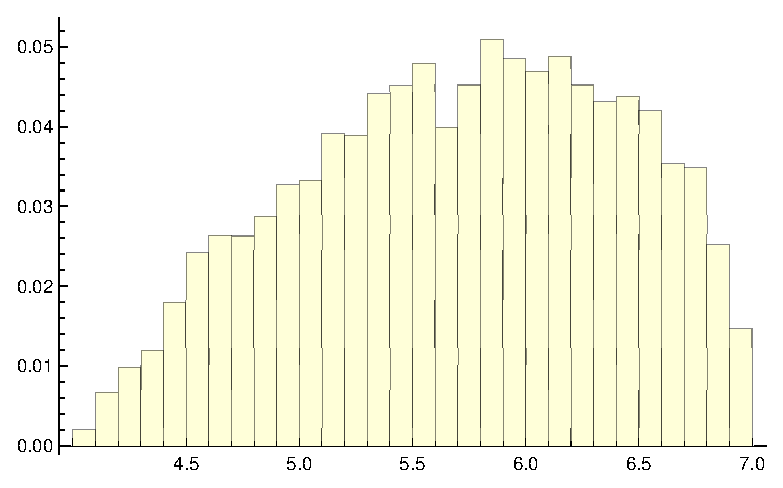
\includegraphics[width=0.95\textwidth]{chapter/prelim-2/D2}
			\subcaption{}
			\label{chapter:prelim-2:example-2-a}
		\end{subfigure}
		\quad
		\begin{subfigure}[b]{0.45\textwidth}
			\centering
			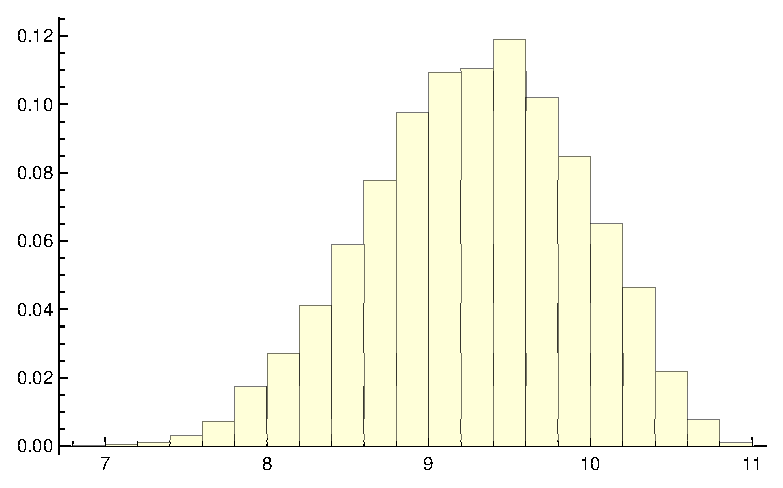
\includegraphics[width=0.95\textwidth]{chapter/prelim-2/cmax}
			\subcaption{}
			\label{chapter:prelim-2:example-2-b}
		\end{subfigure}
		\caption{Sampling the distribution of task 2 (a) and the makespan distribution (b).}
		\label{chapter:prelim-2:example-2}
	\end{figure}

	Obtaining such a histogram `approximation' of the makespan distribution can be accomplished with the following straightforward process.
	First, a topological order of the task network is computed with an algorithm like \cite{tarjan1976}.
	Then, a sufficiently large number of realizations (or scenarios) of random vector $D=(D_1,\ldots,D_n)$ is generated,
	which can be trivial when $D_i$ are independent random variables.
	Finally, the realized schedule for each generated scenario can be computed with Eq.~\ref{chapter:prelim-2:sj} by visiting each task in topological order.
	
% the pert problem in vlsi design
	\subsection{The makespan distribution problem in VLSI}
	In addition to project scheduling, 
	computing the makespan distribution turns out to be important in the design of Very Large Scale Integration (VLSI) circuits.
	This problem emerges because a digital circuit can be modelled as a stochastic task network.
	Nodes correspond to gates (instead of tasks) and precedence constraints corresponding to wiring.
	The equivalent of a task duration is now the amount of time needed by a gate to prepare its output.
	Due to manufacturing imperfections, the latter varies randomly across the chip surface,
	and under certain conditions we may assume to know its probability distribution.
	Makespan corresponds to the length of the clock cycle and computing its distribution
	allows us to compute the \emph{yield} -- the probability that a certain percentage of manufactured chips satisfy certain timing criteria.

	Computing the makespan distribution has received significant additional attention
	since the relatively recent discovery of its important role in the industry of circuit design \cite{blaauw2008}.
	The continuously growing area of so-called \emph{Statistical Timing Analysis} (STA) includes
	a variety of efficient techniques for accurately estimating the distribution of networks with millions of nodes.
	STA techniques range from propagating analytical expressions of the distribution through the network \cite{visweswariah2006}
	to sophisticated Monte Carlo sampling \cite{veetil2011}.
	The use of STA techniques in large-scale project scheduling problems has been studied at least in \cite{mountakis2013}.

% scheduling policies
\section{Scheduling policies}
	Turning our attention back to scheduling,
	in some applications tasks occuppy certain amounts of one or more resources during their execution.
	The resource demands of tasks and the capacities of available resources are known together in scheduling as \emph{resource constraints}.
	Note that one or more tasks which are not precedence-related may execute in parallel.
	Such a combination of tasks the total resource demands of which would exceed resource capacities in case they overlapped in time, 
	is often known as a \emph{forbidden set}.
	For a more comprehensive summary of resource constraints,
	the reader may refer to Section~\ref{chapter:prelim-1:resource-constraints}.
	
	\begin{example}
		Consider the example task network in Figure~\ref{chapter:prelim-2:example-1} and assume, 
		for tasks 2,4 and 5, that each requires the use of a repair platform during its execution.
		If in addition we assume there are only two platforms available, then tasks 2, 4 and 5 form a forbidden set.
		Consider the two schedules formed by earliest start dispatching and shown in Figure~\ref{chapter:prelim-2:example-1b}.
		Neither schedule is feasible as both allow the three tasks to overlap within intervals $[5, 6]$ and $[9, 11]$, respectively,
		over-subscribing to the repair platform resource.
	\end{example}

	Given a stochatic task network along with resource constraints,
	an emerging problem is to define a dispatching strategy that minimizes \emph{expected makespan} while preventing a forbidden set from overlapping during execution,
	ensuring the realized schedule satisfies both precedence and resource constraints.
	Note that earliest-start dispatching is generally not such a strategy, 
	since it only accounts for precedence constraints.
	M\"ohring et al. have studied possible classes of such dispatching strategies,
	known as \emph{scheduling policies} \cite{mohring1984stochastic,mohring1985stochastic}.%
	\footnote{From this point on, the terms scheduling policy and dispatching strategy shall be used interchangeably.}
	A computational study examining the potential superiority of certain classes was conducted by Stork in \cite{stork2000branch}, 
	based on exact branch-and-bound procedures.
	Recently, a new exact method was proposed in \cite{creemers2015minimizing} and
	other authors investigated (meta-)heuristics for minimizing expected makespan \cite{ashtiani2011new, ballestin2009resource}.

% es-policies and partial order schedules 
	We have already encountered a class of scheduling policies, back in Chapter~\ref{chapter/prelim-1}.
	More specifically, in Section ~\ref{chapter:prelim-1:resource-constraints} we discussed how given a network of termporal constraints along with resource constraints,
	we can eliminate forbidden sets by adding precedence constraints to form a so-called partial order schedule (or POS for short).
	Partial order schedules are almost identical to so-called \emph{earliest start policies}.
	The difference between an earliest start policy and a partial order schedule is subtle.
	Partial order schedules are discussed in the context of STP constraints between pairs of tasks,
	while earliest start policies are discussed in the context of simple precedence constraints.
	Just as a network of precedence constraints is a special case of a STP, 
	it could be argued, then, that an earliest start policy is a special-case of a partial order schedule.
	We demonstrate the concept of an earliest start policy with the following example.

	\begin{example}
		In our previous example, we saw that tasks 2, 4 and 5 form a forbidden set and as such,
		their execution should not overlap at any point in time in a feasible schedule.
		To prevent these tasks from overlapping, 
		it suffices to add a precedence constraint between any two members of the forbidden set $\{2,4,5\}$.
		Recall that a precedence constraint is a directed arc $(i, j)$, meaning that $j$ has to wait for the completion of $i$.
		Adding any of the constraints enumerated below would turn our example task network into an earliest start policy,
		the dispatching of which is guaranteed to produce a schedule satisfying both precedence and resource constraints, regardless of outcome task durations.
		\begin{enumerate}
			\item $(2,4)$, yielding an expected makespan of 11.4 hours
			\item $(4,2)$, yielding an expected makespan of 14.5 hours
			\item $(2,5)$, yielding an expected makespan of 11.4 hours
			\item $(5,2)$, yielding an expected makespan of 14.5 hours
			\item $(4,5)$, yielding an expected makespan of 11.4 hours
			\item $(5,4)$, yielding an expected makespan of 11.4 hours
		\end{enumerate}
		Note that without adding any of the constraints listed above, we observe an expected makespan of 9.2 hours.
		Clearly, delaying the dispatching of task 2 (by adding either $(4,2)$ or $(5,2)$) is not preferrable, 
		as it results in the largest expected makespan increase.
	\end{example}

% the concept of stability
\section{Stability and robustness}
\label{chapter:prelim-2:stability}
	Dispatching a stochastic task network (with a scheduling policy) in order to minimize expected makespan 
	is said to maximize \emph{quality-robustness}, or simply robustness.
	All works cited so far focus on finding a policy of optimal quality-robustness.
	Optimizing quality-robustness alone, however, is not always a suitable objective.
	Next to quality robustness,
	in certain applications it is also important to have a \emph{predictive schedule} 
	from which the realized schedule is not expected to deviate too far.
	Without such a predictive schedule offering visibility into the future,
	human and other types of resources cannot plan ahead in order to be in the right place, at the right time.
	The quality of such a predictive schedule to remain close to the realized schedule
	is often known in scheduling literature as \emph{solution-robustness} or \emph{stability} \cite{bidot2009, van2006trade}.

	\begin{example}
		Figure~\ref{chapter:prelim-2:example-3-a} shows (a histogram of) the resulting dispatching times for tasks 2, 3, 4 and 5 
		of the network in Figure~\ref{chapter:prelim-2:example-1} when using earliest start dispatching 
		and assuming durations follow the Beta distribution as described earlier.
		The dispatching time of task 1 is ommitted, as it has no predecessors to wait for and can thus always start at time 0.
		Clearly, the outcome dispatching times are rather unpredictable.
		Task 4, for instance, may start anywhere between time 4 and 8,
		with each of the possible start times having a chance of at most 10\% of being observed.
		It is therefore impossible to plan ahead for the participation of human and other types of resources.
	\end{example}

	The unpredictability of future dispatching times in the workshop can, in fact, be controlled
	with an approach sometimes known as \emph{railway scheduling} \cite{van2005use}.
	Given a task network and a scheduling strategy (if resource constraints are present),
	this approach amounts to defining a predictive dispatching time, per task, and 
	modifying the dispatching process to force the outcome dispatching times to remain close to predictive ones.
	More in particular, each task $j$ is associated with a respective predictive dispatching time $t_j$.
	Whatever dispatching strategy is in use must then observe this additional restriction:
	task $j$ may not be dispatched before $t_j$, even if doing so would not violate any temporal or resource constraints.
	%In case of earliest start dispatching (e.g. when no resource constraints are given, or when using an earliest start policy),
	%instead of starting a task $j$ immediately when its predecessors finish (i.e. according to Eq.~\ref{chapter:prelim-2:sj}),
	%we would also account for its associated predictive schedule time $t_j$, as follows:
	%\begin{align}
	%	S_j := \max \left\{ t_j, \max \{S_i + D_i : i \textrm{ is a predecessor of } j\}  \right\} \label{chapter:prelim-2:sj-stable}
	%\end{align}

	\begin{figure}
		\centering
		\begin{subfigure}[b]{0.95\textwidth}
			\centering
			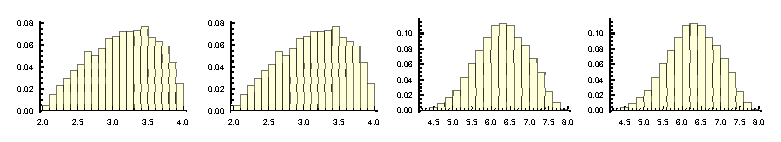
\includegraphics[width=0.95\textwidth]{chapter/prelim-2/row1}
			\subcaption{No predictive schedule.}
			\label{chapter:prelim-2:example-3-a}
		\end{subfigure}
		
		\begin{subfigure}[b]{0.95\textwidth}
			\centering
			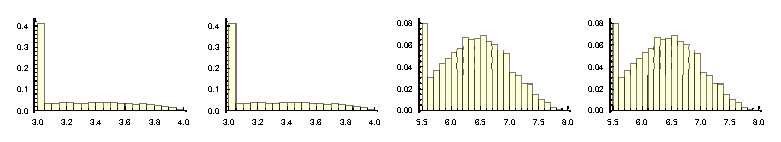
\includegraphics[width=0.95\textwidth]{chapter/prelim-2/row2}
			\subcaption{Using predictive schedule $t_1 = 0, t_2 = 3.0, t_3 = 3.0, t_4 = 5.5, t_5 = 5.5$.}
			\label{chapter:prelim-2:example-3-b}
		\end{subfigure}

		\begin{subfigure}[b]{0.95\textwidth}
			\centering
			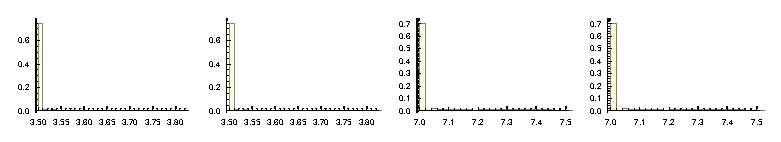
\includegraphics[width=0.95\textwidth]{chapter/prelim-2/row4}
			\subcaption{Using predictive schedule $t_1 = 0, t_2 = 3.5, t_3 = 3.5, t_4 = 7.0, t_5 = 7.0$.}
			\label{chapter:prelim-2:example-3-c}
		\end{subfigure}
		\caption{Histogram representation of the realized dispatching times for tasks 2, 3, 4 and 5 (with task 1 always dispatched at time 0) for our example task network,
		when using earliest start dispatching with and without a predictive schedule.
		As predictive start times are spread farther apart, start time variability diminishes.}
		\label{chapter:prelim-2:example-3}
	\end{figure}

	As better illustrated in the following example,
	as those predictive (or minimum) start times are spread along the time-axis, 
	unpredictability diminishes (or stability improves) and outcome dispatching times tend to stay close to predictive ones.
	In effect, then, vector $(t_1, t_2, \ldots, t_n)$ constitutes a reliable predictive schedule that can be used for planning ahead.

	\begin{example}
		Figure~\ref{chapter:prelim-2:example-3-b}
		shows what happens when earliest start dispatching is used with the additional rule that
		tasks 2, 3, 4 and 5 cannot start before $t_2 = 3.0, t_3 = 3.0, t_4 = 5.5$ and $t_5 = 5.5$, respectively.
		Clearly, the start times of tasks 2 and 3 become more predictable,
		with a start time of $t_2 = t_3 = 3.0$ for tasks 2 and 3 having a relatively high chance of being observed, at 40\%. 
		Unfortunately, the start times of tasks 4 and 5 remain unpredictable.
		Figure~\ref{chapter:prelim-2:example-3-c} shows how stability improves when the predictive schedule is spread farther apart in time,
		yielding, for each task, a chance of about 70\% to start at its predictive start time.
		Moreover, note how even if a task does not start at its predictive time, it will most likely start somewhere near. 
		Tasks 4 and 5, for instance, might start with a delay of at most 0.5 hours from their predictive time.
		Enhancing stability, however, has an impact on performance.
		When not using a predictive schedule at all (i.e. Figure~\ref{chapter:prelim-2:example-3-a}) the expected makespan is at 9.2 hours.
		Using the predictive schedule in Figure~\ref{chapter:prelim-2:example-3-b}, expected makespan increases only slightly at 9.4 hours.
		Ultimately, using the stable predictive schedule in Figure~\ref{chapter:prelim-2:example-3-c} yields an expected makespan of 9.9 hours.
	\end{example}

	%When the focus is exclusively on minimizing expected makespan, however, 
	%the realized schedule (i.e. the outcome task start times) is mostly unpredictable.

	As demonstrated in our previous example,
	scheduling tasks efficiently and scheduling tasks predictably 
	(or optimizing quality-robustness and solution-robustness) are usually conflicting objectives \cite{van2006trade}.
	A relatively small research area  within the literature, known as \emph{proactive-reactive project scheduling},
	focuses on problems for which the solution is a pair formed by a scheduling policy and a predictive schedule.
	The objective is to find such a pair offering an optimal \emph{trade-off} between quality-robustness and stability.
	The work presented in Chapters 6 and 7 of this dissertation focuses on the problem of trading robustness for stability.

% research questions
\section{Research Questions}
\label{chapter:prelim-2:research-questions}
	In this Section we discuss how existing work, summarized in preceeding sections,
	can help us address Research Problem II, stated in Chapter~1.
	In doing so, we raise appropriate Research Questions that map to gaps in existing literature.
	The raised questions are eventually addressed in Chapters 6 and 7.

	% RP statement and policies as robust schedules
	Referring back to Research Problem II, 
	we would like to compute robust and stable schedules for work-teams,
	in order to deal with uncertainty in the duration of maintenance tasks.
	A robust schedule should guarantee good performance under a variety of possible outcome duration scenarios.
	Owing to the recurrent nature of maintenance operations,
	we are able to gather data over past maintenance sessions and build, for each task duration, 
	a probability distribution according to which it varies over different executions.
	Given the description of each task duration as a random variable with a known distribution,
	a scheduling policy is functionally equivalent to a robust schedule,
	as it provides a set of rules for deriving appropriate dispatching times by reacting to observed task durations,
	such that feasibility and good performance are both guaranteed over a range of possible scenarios.

	% the need for stability
	As explained in Section~\ref{chapter:prelim-2:stability}, however, robustness alone is not always sufficient.
	Next to ensuring good performance under a variety of potential scenarios and taking the human factor into account, 
	we would also like to offer stability, or visibility of future dispatching times.
	That is, we would also like to force and/or predict that outcome dispatching times will fall within certain time-windows,
	or near certain predictive dispatching times. 
	Such a stable or predictive schedule is necessary for planning-ahead the availability of human and other resources
	in the right place and at the right time in the workshop.

	% coverage by existing literature
	Modern literature on stochastic project scheduling addresses the problem of balancing robustness and stability
	with techniques for computing a scheduling policy along with a reliable predictive schedule.
	Existing approaches, however, suffer from certain limitations,
	as they tend to treat the scheduling policy and the predictive schedule separately.
	The prominent paper by Van de Vonder et al. \cite{van2008}, for instance, 
	treats the optimization of a policy and predictive schedule separately, in a-two step fashion,
	while the exact approach of \cite{lamas2015} follows a policy-agnostic approach, 
	optimizing the predictive schedule without assuming anything about the structure of the policy.
	Considering, instead, the problem as a whole such that the structure of the policy is taken into account when choosing the predictive schedule, and vice-versa,
	gives us access to a solution-space of higher dimensionality.
	Since performance is determined in practice by the policy and the predictive schedule together,
	in pursuit of potentially better results we would like to address the following question:
		
		\begin{rquest}
			\label{rquest-2-1}
			How to optimize a scheduling policy and a predictive schedule together as a pair?
		\end{rquest}

	% RP: diminishing of uncertainty
	Moreover, as time progresses and outcome dispatching times and task durations are being observed, 
	uncertainty gruadually diminishes in the workshop.
	As such, we are presented with an opportunity to adapt to new information accordingly by rescheduling.
	In order to keep pace with execution and to avoid introducing further delays,
	the computational effort spent in rescheduling should be rather limited in practice. 
	Therefore, during rescheduling we should avoid reconsidering the structure of the scheduling policy,
	in order to avoid the combinatorial explosion associated with reasoning about resource constraints.
	It might, however, be fruitful to react to new information by adapting the predictive schedule.
	As such, we are interested in addressing the following question:

		\begin{rquest} 
			\label{rquest-2-2}
			How to update the predictive schedule by reacting to outcome durations in low order polynomial time, keeping pace with execution?
		\end{rquest}

	Research Question~\ref{rquest-2-1} is answered in Chapter~6.
	In the first part of Chapter~6, we present a linear programming (LP) approach for finding a predictive schedule offering an optimal 
	trade-off between makespan and stability, given a fixed earliest start policy.
	In the second part we develop a Mixed Integer LP extension of our approach which enables 
	us to optimize an earliest start scheduling policy together with the predictive schedule.
	Research Question~\ref{rquest-2-2} is answered in Chapter~7.
	There, we present a dynamic programming algorithm which can function as a much faster alternative to the LP approach developed in Chapter 6.


\chapter[Stable dispatching with resource constraints]{Stable dispatching with resource constraints\protect\footnotemark{}\protect\footnotetext{
This chapter has been published as:
K.S. Mountakis, T.B. Klos, C. Witteveen, and B. Huisman. Exact and heuristic methods for trading-off makespan and stability in stochastic project scheduling. 
In \emph{Multidisciplinary International Scheduling Conference: Theory and Application (MISTA)}, pages 25-41, 2015.}}

\label{chapter/mista-stability}
%%%%%%%%%%%%%%%%%%%%%%%% file template.tex %%%%%%%%%%%%%%%%%%%%%%%%%
%%
%% This is a general template file for the LaTeX package SVJour3
%% for Springer journals.          Springer Heidelberg 2006/03/15
%%
%% Copy it to a new file with a new name and use it as the basis
%% for your article. Delete % signs as needed.
%%
%% This template includes a few options for different layouts and
%% content for various journals. Please consult a p revious issue of
%% your journal as needed.
%%
%%
%% 5th Mar 2012
%% NOTES for MISTA 2015
%% This template has been supplied for use for the MISTA 2015 conference
%% In essence it is the same as the one supplied by SV, but with additional comments
%% The reason this template is being used is to make it as easy as possible
%% to be able to submit to the post conference special issue of the Journal
%% of Scheduling
%%%%%%%%%%%%%%%%%%%%%%%%%%%%%%%%%%%%%%%%%%%%%%%%%%%%%%%%%%%%%%%%%%%%
%%
%% First comes an example EPS file -- just ignore it and
%% proceed on the \documentclass line
%% your LaTeX will extract the file if required
%\begin{filecontents*}{example.eps}
%%!PS-Adobe-3.0 EPSF-3.0
%%%BoundingBox: 19 19 221 221
%%%CreationDate: Mon Sep 29 1997
%%%Creator: programmed by hand (JK)
%%%EndComments
%gsave
%newpath
%  20 20 moveto
%  20 220 lineto
%  220 220 lineto
%  220 20 lineto
%closepath
%2 setlinewidth
%gsave
%  .4 setgray fill
%grestore
%stroke
%grestore
%\end{filecontents*}
%%
%% For MISTA 2015, use the default option that has been supplied
%\documentclass{svjour3}                     % onecolumn (standard format)
%%\documentclass[smallextended]{svjour3}     % onecolumn (second format)
%%\documentclass[twocolumn]{svjour3}         % twocolumn
%%
%\smartqed  % flush right qed marks, e.g. at end of proof
%%
%\usepackage{graphicx}
%%
%% \usepackage{mathptmx}      % use Times fonts if available on your TeX system
%%
%% insert here the call for the packages your document requires
%\usepackage{latexsym}
%\usepackage{amsmath}
%\usepackage{amsfonts}
%\usepackage{graphicx}
%\usepackage{subfig}
%\usepackage{algorithmic}
%\usepackage{algorithm}
%\usepackage{enumerate}
%\usepackage{microtype}
%\usepackage{multirow}
%
%% please place your own definitions here and don't use \def but
%% \newcommand{}{}
%
%\newcommand{\xsc}{\gamma}
%\newcommand{\xSC}{\Gamma}
%
%\newcommand{\xs}{\boldsymbol{s}}
%\newcommand{\xd}{\boldsymbol{d}}
%\newcommand{\xq}{\boldsymbol{q}}
%\newcommand{\xb}{\boldsymbol{b}}
%\newcommand{\xl}{\boldsymbol{l}}
%\newcommand{\xf}{\boldsymbol{f}}
%\newcommand{\xD}{\boldsymbol{D}}
%\newcommand{\xt}{\boldsymbol{t}}
%\newcommand{\xe}{\epsilon}
%
%\newcommand{\xE}{\mathcal{E}}
%\newcommand{\xS}{\boldsymbol{S}}
%\newcommand{\xX}{\boldsymbol{X}}
%\newcommand{\xP}{\boldsymbol{\Pi}}
%\newtheorem{edit}{Edit}	
%\newtheorem{TODO}{TODO}
%
%% Insert the name of "your journal" with
%% This is preset for MISTA 2015: Do not change
%\journalname{MISTA 2015}
%%
%\setcounter{tocdepth}{3}
%\begin{document}
%
%\title{Exact and heuristic methods for trading-off makespan and stability in stochastic project scheduling} 
%\subtitle{}
%
%\author{Simon Mountakis \and
%	Tomas Klos \and \\
%	Cees Witteveen \and
%	Bob Huisman
%}
%
%\institute{Simon Mountakis \at
%	      Delft University of Technology \\
%	      \email{k.s.mountakis@tudelft.nl}  %  \\
%	   \and
%	   Tomas Klos \at
%	      Delft University of Technology \\
%	      \email{t.b.klos@tudelft.nl}  %  \\
%	   \and
%	   Cees Witteveen \at
%	      Delft University of Technology \\
%	      \email{c.witteveen@tudelft.nl}  %  \\
%	   \and
%	   Bob Huisman \at
%	      NedTrain \\
%	      \email{b.huisman@nedtrain.nl} %  \\
%}
%
%\maketitle
%
%\begin{abstract}
%This paper addresses a problem of practical value in project scheduling:
trading expected makespan for stability,
under stochastic activity duration uncertainty.
We present the formal statement of a problem 
that we name Proactive Stochastic RCPSP (PS-RCPSP).
Assuming activity durations follow known probability distributions,
PS-RCPSP asks to find a so-called earliest-start (es) policy and
a proactive schedule that together minimize the weighted 
sum of expected project makespan and expected instability
(deviation of the realized from the proactive schedule).
%
Extending an existing MILP model for the well-known deterministic 
Resource-Constrained Project Scheduling Problem (RCPSP),
we present a MILP model for PS-RCPSP, which allows us to 
find optimal (es-policy, proactive schedule) pairs.
To deal with instances of practical size,
we propose a Linear Programming (LP)-based 
and a Mixed-Integer LP (MILP)-based heuristic.
Our LP-based heuristic optimizes the proactive schedule while 
keeping the es-policy part of the solution fixed.
Our MILP-based heuristic aims to optimize the structure of the policy together with the proactive schedule.
In contrast to existing state-of-art approaches such as
CCP \cite{lamas2014purely} and STC \cite{van2008},
our heuristics rely on optimizing the proactive schedule together with the scheduling policy.
%
Experiments show that the LP-based heuristic is efficient and compares favorably with the state-of-art 
(i.e.\ achieves smaller expected makespan for a certain level of expected instability)
when the aim is to achieve near-zero instability at the cost of higher makespan.
The MILP-based heuristic seems more effective (albeit not as efficient) when the aim is to
achieve low expected makespan at the cost of moderate or high instability.

%\end{abstract}
%
%%	\tableofcontents
%
\section{Introduction}
	
	% -- deterministic RCPSP
	
	Project scheduling literature mostly concentrates on scheduling
	subject to temporal and resource constraints.
	The schedule sought for is an assignment of start-times to activities,
	facilitating the efficient use of limited resources
	in order to minimize a lateness measure such as the project makespan.
	Finding a schedule usually invovles solving
	the Resource-Constrained Project Scheduling Problem (RCPSP) 
	(see \cite{artigues2013resource,hartmann2010survey} for comprehensive surveys).
	This problem has been shown to be \textsc{NP}-Hard \cite{blazewicz1983scheduling} and
	finds several industrial applications (e.g. \cite{bomsdorf2008model,bartels2009scheduling}).
	Associated literature includes numerous exact and (meta-)heuristic algorithms,
	able to find good schedules for large instances and diverse lateness measures
	(e.g. \cite{schutt2013solving,kone2011event,kolisch2006experimental,de2014novel}).
	%
	% -- transition from RCPSP to S-RCPSP because of uncertainty
	%
	Solving an RCPSP serves the purpose of preparing a feasible schedule,
	assuming a static deterministic project execution environment.
 	In practice, however, this assumption is rarely valid.
 	Activity durations used for preparing the schedule are mostly rough estimates,
 	since most projects are subject to delays during execution and
 	the final realized schedule is the result of 
 	subjecting the original schedule to modifications
 	which make it consistent with the project constraints in the face of delays.
 	Ad-hoc modifications lead to realized activity start-times 
 	that might differ from planned start-times,
  	compromising project predictability and timeliness.
	
	This paper addresses the issue of hedging against project uncertainty 
 	by preparing a schedule in combination with an execution strategy for coping with delays.
	In line with other works in \emph{stochastic project scheduling} 
	(see \cite{herroelen2004robust} for a comprehensive review)
	we assume activity durations are given as stochastic variables with known distributions
	and propose a new \emph{proactive-reactive} scheduling method.
	First, we define the Proactive Stochastic (PS) RCPSP as an extension of RCPSP.
	The solution to PS-RCPSP is a \emph{proactive schedule} and an \emph{earliest-start (es-) policy}
	that together minimize the weighted sum of the realized schedule's expected makespan 
	and its expected deviation from the proactive schedule.
	%
	PS-RCPSP is, in fact, a generalization of the Stochastic RCPSP (S-RCPSP),
	which asks to find a \emph{stochastic scheduling policy} instead of a schedule
	and various \emph{classes} of policies have been proposed in the literature 
	\cite{mohring1984stochastic,mohring1985stochastic,herroelen2004robust}.
	In general, a  policy defines a mapping between activity duration realizations to realized schedules.
	S-RCPSP asks to find a policy that minimizes the expected project makespan,
	with only few exact and heuristic approaches (mainly meta-heuristics) proposed over the last decade
	\cite{stork2000branch,ballestin2007worthwhile,ballestin2009resource,ashtiani2011new}.	
	
	Not preparing the project execution based on a schedule that can more or less be trusted
	(but rather, letting the realized schedule unfold during execution) 
	has been recognized as a shortcoming of S-RCPSP \cite{herroelen2004construction}.
	This shortcoming motivates us and a number of 
	other authors to propose a proactive-reactive approach,
	with \cite{van2008,deblaere2011proactive,lamas2015}
	yielding the most promising computational results in existing literature.
	Different approaches pursue different optimization objectives;
	however, the common aim is to optimize some \emph{tradeoff} between expected makespan 
	and expected deviation from the proactive schedule.
 	In line with other authors we represent activity duration distributions with a sample
 	and propose a Linear Programming (LP)-based heuristic for PS-RCPSP,
 	a Mixed-Integer LP (MILP) model enabling us to obtain exact solutions, and
 	a MILP-based heuristic which asimilates \emph{iterative flattening} \cite{oddi2009iterative}.
   	The (MI)LP models for PS-RCPSP proposed in this paper are the 
 	result of adjusting the models proposed by Artigues et al. in
 	\cite{artigues2003insertion} and \cite{leus2011robust}.	
 	We refer to exact solutions assuming stochastic duration distributions 
 	can be represented exactly by a sufficiently large sample.\footnote{
 	This notion of exactness is in line with Stork \cite{stork2000branch} who 
 	represent stochastic duration distributions with a sample
 	when proposing exact search methods for the S-RCPSP.}
 	
 	
%%%	Following the definition of PS-RCPSP we propose a heuristic based on Linear Programming (LP),
%%%	a Mixed Integer LP (MILP) model for PS-RCPSP that enables the finding exact solutions, and
%%%	a MILP-based heuristic that involves solving a sequence of smaller subproblems.
%%%	Similar proactive-reactive scheduling methods have been proposed by a number of authors,
%%%	with the heuristics in \cite{van2008,deblaere2011proactive,lamas2015} 
%%%	giving the most promising computational results.
%%%	Experiments with the known PSPLIB benchset \cite{kolisch1997psplib}
%%%	show that our heuristics compare favorably with prior art.
%%%	
%%%	This paper addresses the issue of hedging against project uncertainty 
%%% 	by preparing a schedule in combination with an execution strategy for coping with delays and
%%%	assuming activity durations are stochastic variables with known probability distributions.
%%% 	We propose a Mixed Integer Linear Programming (MILP) model along with two associated heuristics
%%% 	for a ploblem that we name the Proactive Stochastic RCPSP (PS-RCPSP).
%%% 	PS-RCPSP is, in fact, a generalization of an extension to the RCPSP,
%%% 	known as the Stochastic RCPSP (S-RCPSP),
%%% 	which is the main problem of study in the area of stochastic project scheduling \cite{herroelen2004robust}
%%%	(also known as reactive project scheduling).
%%%	S-RCPSP asks to find a \emph{stochastic scheduling policy} instead of a schedule.
%%%	Various \emph{classes} of policies have been proposed in the literature 
%%%	\cite{mohring1984stochastic,mohring1985stochastic,herroelen2004robust} but in general,
%%%	a policy is a combinatorial object representing a set of rules
%%%	that may guide the materialization of a final realized schedule,
%%%	as actual activity durations become known during project execution.
%%%	In effect, the policy defines a mapping from
%%%	every possible realization of activity durations to a corresponding realized schedule.
%%%	S-RCPSP asks to find a policy that minimizes the expected value of some project lateness measure
%%%	(e.g. the expected project makespan).
%%%	Few exact and heuristic S-RCPSP solution algorithms have been developed over the last decade
%%%	\cite{stork2000branch,ballestin2007worthwhile,ballestin2009resource,ashtiani2011new}.
%%%	
%%%	% -- transition from S-RCPSP to PS-RCPSP
%%%	
%%%	A main characteristic of S-RCPSP is that no schedule is prescribed prior to project execution.
%%%	Activity start-times are determined in a purely dynamic manner by the scheduling policy.
%%%	This has been recognized as a drawback (e.g. \cite{herroelen2004construction}) 
%%%	since the existence of a \emph{proactive}
%%%	schedule that can more or less be trusted may serve important organizational purposes.
%%%	An attempt to overcome this drawback gave rise to the research area of proactive-reactive project scheduling
%%%	which  is the research area that our work belongs to.
%%% 	The main idea behind the proactive-reactive approach is to execute the project by using
%%%	a proactive schedule together with a scheduling policy.
%%% 	The general aim of prominent approaches in this area 
%%%  	(e.g. \cite{van2008,deblaere2011proactive,lamas2015}) is to
%%% 	optimize some tradeoff between expected makespan and 
%%%	expected instability (deviation of the realized from the proactive schedule).
%%%		
%%%	The problem studied here, the PS-RCPSP, asks to find
%%%	a \emph{proactive} schedule paired with an \emph{earliest-start} (es) policy.
%%%	An es-policy is a set of temporal constraints between pairs of activities.
%%%	The proactive schedule prescribes release-times 
%%%	(i.e. earliest possible start-times) for activities.
%%%	An activity may start at its prescribed release-time or later in case of delays
%%%	(i.e. other activities requiring more than allocated time) as determined by the es-policy.
%%%	In effect, the tuple (proactive schedule, es-policy) defines a mapping from
%%%	every possible realization of activity durations to a corresponding realized schedule.
%%%	PS-RCPSP asks to find this tuple that minimizes 
%%%	the \emph{weighted sum} of two performance criteria:
%%%	\begin{enumerate}
%%%		\item expected project makespan,
%%%		\item expected tardiness with respect to the proactive schedule.
%%%	\end{enumerate}
%%%	The first criterion is relevant for obvious reasons.
%%%	The second criterion represents the extent to which the proactive start-times can be trusted.
%%% 	One typically wants to achieve low instability to avoid what is
%%% 	known as \emph{nervousness} \cite{steele1975nervous} and induces organizational costs.
 	
 	% -- paper structure and contributions
 	
	%This paper is about a problem of practical value in project scheduling:
	%trading expected makespan for stability under stochastic uncertainty.
	
	The contributions of this paper extend from section~\ref{sec-problem} and onwards.
	In order to base the paper on a consistent and self-contained framework of notation,
	section~\ref{sec-prelim} summarizes existing concepts from
	deterministic, reactive, and proactive-reactive project scheduling.
 	Section~\ref{sec-problem} introduces in a formal manner the problem studied here,
 	that we name Proactive Stochastic RCPSP.
	Section~\ref{sec-lp} presents one main contribution of this paper:
	a LP-based heuristic for solving this problem.
 	Section~\ref{sec-milp} presents another main contribution:
 	a MILP model for this problem which enables us to obtain exact PS-RCPSP solutions.
 	To our knowledge, no other exact solution methods have been proposed for poblems of similar type.
	Section~\ref{sec-milp-heuristic} presents yet another contribution,
	a MILP-based heuristic for PS-RCPSP.
	Section~\ref{sec-experiments} presents an experimental study in which we find
	that the LP-based heuristic performs favorably in comparison to the state-of-art,
	especially when the aim is to achieve near-zero instability.
	We also find the MILP-based heuristic to be more effective (albeit less efficient)
	when one is willing to accept medium levels of instability in order to minimize expected makespan.
	Section~\ref{sec-conclusion} concludes the paper.	
 	

\section{Preliminaries}
	\label{sec-prelim}
 	
 	The purpose of this section is to introduce the research area of
 	proactive-reactive (stochastic) project scheduling,
 	which is where the contributions of this paper belong to.
  	To establish autonomy and to facilitate discussion in further sections,
  	we use convenient notation (which sometimes departs from standard notation)
  	and begin with summarizing existing concepts from 
  	deterministic and (purely) reactive project scheduling.
  	For a comprehensive survey of deterministic,
  	reactive and proactive-reactive project scheduling,
  	the reader may refer to \cite{herroelen2004robust}.
   	 	
 	\subsection{Deterministic project scheduling}
 	 	
	A project is usually represented as a directed acyclic graph $G(N,E)$,
	with nodes $N=\{1,\ldots,n\}$ corresponding to the set of $n$ project activities.
	Each directed arc $(i,j)$ in $E \subseteq \{(i,j) \in N^2\}$ defines a direct
	temporal constraint between activities $i$ and $j$,
	meaning that $j$ may not start unless activity $i$ has finished.
 	In effect, $E$ defines a binary, irreflexive and transitive relation:
 	if there is a path from activity $i$ to activity 
 	$j$ in $G(N,E)$ then $j$ cannot start unless $i$ has finished.
	Let us $T(E) \supseteq E$ denote the transitive closure of $E$, 
	defined as 
	\[
		T(E) := \{(i,j) \in N^2 : \exists 
		\textrm{ a path from } i \textrm{ to } j \textrm { in } G(N,E)\}
	\]
	We shall name a \emph{temporally independent set} each
	subset of activities $X \subseteq N$ which are mutually 
	independent with respect to temporal constraints.
	That is, if $X$ is a temporally independent set, then $X^2 \cap T(E) = \emptyset$.
	Obviously, if only temporal constraints are taken into account, 
	the activities of a temporally independent set may overlap in time in a schedule.
	
	We assume as input a set $R := \{1,\ldots,m\}$ of $m$ resources which must be shared among activities.
	Each resource $r \in R$ is associated with known capacity $b_r \in \mathbb{N}_0$.
	Furthermore, each activity $i \in N$ requires a known amount 
	$q_{ir} \leq b_r$ of resource $r$ while it executes.
	Vector $\xb \in \mathbb{N}^m_0$ and matrix $\xq \in \mathbb{N}^{n \times m}_0$
	define the problem's resource constraints.
	Every independent set $X$ for which $\sum_{i\in X} q_{ir} > b_r$ 
	for some $r\in R$ is called a \emph{forbidden} set.
	Even though it is allowed by the temporal constraints $E$, 
	all activities in $X$ may not overlap at some timepoint $t$ because
	resource $r$ will be used beyond its capacity, which is not possible.
	
	Let $H \subseteq N^2$ denote a set of temporal constraints.
	Below we give the definition of a function $\Phi$ which returns the set of all forbidden sets
	w.r.t. temporal constraints $H$ and the problem's resource constraints $(\xq,\xb)$.
	\begin{align}
		\Phi(H) := \{X \subseteq N: 
		X^2 \cap T(H)=\emptyset, 
		\sum_{i\in X} q_{ir} > b_r \textrm{ for some } r \in R\}
	\end{align}
	
	In addition to the parameters mentioned so far,
	we assume as input a vector $\xd \in \mathbb{N}^n_0$ such that $d_i$ defines the duration of activity $i$.
	Overall, a tuple $(N,R,E,\xd,\xq,\xb)$ specifies an instance of the RCPSP.
	A schedule $\xs \in \mathbb{N}^n_0$ 
	such that $s_i$ defines the start time of activity $i$,
	is a feasible solution when it satisfies the temporal and resource constraints,
	meaning that
	\begin{align}
		s_j \geq s_i + d_i \qquad & \forall (i,j) \in E \label{eq-precon} \\
		a(\xs, t) \notin \Phi(E)	\label{eq-rescon} & \qquad \forall t \geq 0
	\end{align}
 
	Here, $a(\xs,t) := \{i \in N : t \in [s_i, s_i+d_i)\}$ is the set of
	activities executing at timepoint $t$ according to $\xs$ and $\Phi$ as defined earlier.
	Thus, (\ref{eq-rescon}) ensures there is no timepoint $t$ at which the
	activities of a forbidden set overlap concurrently.
	
	\paragraph{Project source-sink convention.}
	RCPSP asks to find a feasible schedule of minimum makespan
	$C_{\max}(\xs) := \max \{ s_i + d_i : i \in N\}$.
	Most RCPSP-related works assume that the last activity, $n$, 
	is a dummy activity with zero duration (i.e. $d_n = 0$) and that
	it must wait for the completion of every other activity (i.e. $(i,n) \in T(E)$ for every $i \in N-\{n\}$).
	This dummy activity is often known as the project "sink" and it holds that $C_{\max}(\xs) = s_n$.
	Another convention of most RCPSP-related works is that the first activity, 1,
	often known as the project "source" must be waited on by every other activity
	(i.e. $(1,j) \in T(E)$ for every $j \in N-\{1\}$).
	
 	We shall hereafter assume activities 1 and $n$ correspond to the project source and sink, respectively.
 	The RCPSP can now be formally stated as:
	\begin{align}
		\xs^* := \arg \min \{s_n:  (\ref{eq-precon}), (\ref{eq-rescon}), \xs \geq 0 \}
	\end{align}
	
	\subsection{Reactive project scheduling}
 	
	In the research area of stochastic project scheduling,
	the activity durations vector $\xd$ is replaced with a stochastic vector $\xD$ such that $D_i$
	is the stochastic variable representing the uncertain duration of activity $i$,
	with a known probability distribution $\mathbb{P}[D_i = t]$.
	In line with recent works on S-RCPSP,
	we shall denote (elements of) stochastic vectors with a capital symbol.
			
	S-RCPSP is a purely reactive extension of RCPSP.
	The solution sought for is no longer a schedule, but a reactive scheduling policy. 
	A policy is a combinatorial object $\pi$ which parameterizes the mapping  from stochatic vector $\xD$
	to a corresponding realized schedule $\xS(\pi,\xD)$.
	Note that $\xS$ denotes a function which returns a vector of activity start times (of length $n$).
	Furthermore, if a realization $\xd$ of $\xD$ is passed as an argument, 
	then $\xS(\pi,\xd)$ denotes a deterministic vector.
	if $\xD$ is passed as an argument, $\xS(\pi,\xD)$ denotes a stochatic vector.
	
	Different classes of policies have been proposed in the literature
	\cite{mohring1984stochastic,mohring1985stochastic,stork2000branch,ashtiani2011new}.
 	One condition that all policy classes are expected to satisfy is that function
 	$\xS$ complies with the \emph{non-anticipativity constraint}:
	the decision to start activity $i$ at time $[\xS(\pi,\xD)]_i$ cannot rely on information from the feature:
	the value of $[\xS(\pi,\xD)]_i$ must be determined by time $t \leq [\xS(\pi,\xD)]_i$.
	Other features such as the structure of $\pi$ and 
	the definition of function $\xS$ depend on the class under study.
	
 	\paragraph{List-based policies.}
	
	Two classes of policies which are prominent in the literature
	are \emph{resource-based} (rb) policies and \emph{activity-based} (ab) policies,
	also known collectively as \emph{list-based policies}.
	A list-based policy is a priority vector $\xl \in \mathbb{R}^n$ assigning priority $l_i$ to activity $i$.
	Realized schedule $\xS(\xl, \xD)$ is computed by a 
	variant of the well-known parallel schedule-generation-scheme (SGS)
	complying with the non-anticipativity constraint \cite{ballestin2009resource};
	with the SGS definition being slightly different between rb-policies and ab-policies.
%	At $t=0$ and at each subsequent activity completion $t > 0$
%	one starts as many activities as allowed by temporal and resource constraints.
%	A similar class is that of \emph{activity-based} (ab) policies;
%	an ab-policy is again a priority vector.
%	But the behavior of $p$ is now slightly different:
%	a activity may not start at $t$ 
%	(even if temporal and resource constraints allow this) unless 
%	all activities of lower priority have finished by $t$.
%	Note that every realized schedule $\xS(\xl,\xD)$ is feasible, 
% 	since function $\xS$ forces the problem's precedence and resource constraints
% 	regardless of the choice of $\xl$.
 	As far as list-based policies are concerned, S-RCPSP asks to find a vector 
	$\xl \in \mathbb{R}^n$ that minimizes $\mathbb{E}[[\xS(\xl,\xD)]_n]$.
	%
	Stork \cite{stork2000branch} proposes exact branch-and-bound algorithms for both rb and ab-policies.
	Ballest{\'\i}n \cite{ballestin2007worthwhile} proposes
	an efficient genetic algorithm for ab-policies,
 	providing the first computational experience on larger S-RCPSP instances.
	Ballest{\'\i}n and Leus \cite{ballestin2009resource} manage 
	to obtain better results with a 
	Greedy Randomized Adaptive Search Procedure (GRASP), 
	again for the class of ab-policies.
	The best performance (w.r.t. expected makespan minimization)
	has so far been obtained with the more recent work of
	Ashtiani et al. \cite{ashtiani2011new} who propose a GRASP
	for a new class, namely \emph{pre-processing} (pp) policies--%
	a hybrid between rb-policies and es-policies.

 	\paragraph{Earliest-start policies.}
 	
   	An es-policy is a set of temporal constraints $\xE \subseteq N^2$ chosen such that
 	\begin{align}
 		T(\xE) \supseteq E, \label{es-1} \\
 		\Phi(\xE) = \emptyset \label{es-2}, \\
 		G(N,\xE) \textrm{ is acyclic} \label{es-3}
 	\end{align}
 	Condition (\ref{es-1}) ensures that a schedule $\xs$ satisfying
 	$s_j \geq s_i + d_i$ for each $(i,j)\in \xE$ 
 	(here $\xd$ can be any arbitrary choice of activity durations)
 	is feasible with respect to the problem's precedence constraints $E$.
  	Condition (\ref{es-2}) ensures that
  	$\xs$ satisfying $\xE$ implies that it also satisfies resource constraints 
  	prescribed by availabilities $\xb$ and requirements $\xq$ (as described earlier).
 	Condition (\ref{es-3}) ensures that the set of schedules satisfying $\xE$ 
 	(for any arbitrary choice of activity durations $\xd$) is non-empty.
 	
 	When a project is executed according to an es-policy $\xE$,
 	the schedule that is realized, $\xS(\xE,\xD)$, 
 	is what is often known as the \emph{earliest-start} schedule specified by $\xE$.
 	The earliest-start schedule of $\xE$ can be defined as:
 	\begin{align}
 		[\xS(\xE,\xD)]_j := \max \{ [\xS(\xE,\xD)]_i + D_i : (i,j) \in \xE\}
 	\end{align}
 	To put it simply, an activity $j$ starts immediatelly 
 	when all its predecessors in $G(N,\xE)$ have finished.
  	This time quantity (the latest finish time of $j$'s predecessors)
  	is often known as the length of the \emph{critical path} from project source $1$ to activity $j$.
  	As far as es-policies are concerned, the S-RCPSP asks to find some $\xE^*$ which
  	minimizes $[\xS(\xE,\xD)]_n$ (the length of the critical path to the project sink) by expectation:
 	\begin{align}
 		\xE^* := \arg \min \{\mathbb{E}[[\xS(\xE,\xD)]_n] : (\ref{es-1} - \ref{es-3}), \xE \in N^2\}
 		\label{eq-s-rcpsp}
 	\end{align}
  	Constraints $(\ref{es-1} - \ref{es-3})$ enforce the feasibility of any realized schedule
  	with both the precedence and the resource constraints of the problem.
  	
	Stork \cite{stork2000branch} proposed an exact branch-and-bound search for problem (\ref{eq-s-rcpsp}).
	His algorithm considers each \emph{minimal} forbidden set $X$
	(subset-minimal forbidden set) in some order and branches
	on each of $|\{(i,j) \in X^2\}|$ arcs which can be included in $\xE$
	in order to eliminate $X$ from $\Phi(\xE)$.
	Without obtaining new computational results,
	in \cite{leus2011resource} Leus gives a formal treatment of
	es-policies as resource-flow networks
	(flow networks which can represent feasible RCPSP schedules) and
	proposes a refined version of the branch \& bound algorithm of Stork.
	Exploiting the relation between resource-flows and es-policies,
	Artigues et al. \cite{leus2011robust} propose a 
	robust optimization model for es-policies,
	for when a stochastic characterization of uncertainty is not available.
	
\subsection{Proactive-reactive project scheduling}
	
	Reactive project scheduling allows one to pick activity start times dynamically
	during the project, under conditions of uncertainty.
	A main drawback of this approach 
	(e.g. \cite{herroelen2004construction,herroelen2004robust,braeckmans2005proactive})
	is that prior to (and during) project execution there is no 
	schedule prescribing activity start times that can more or less be trusted.
	Such a "proactive" schedule can serve important organizational purposes;
	in fact, the deviation of the realized schedule from this proactive schedule
	is expected to induce organizational costs.
	
	Attempts to overcome this drawback gave rise to the research area of
	proactive-reactive project scheduling,
	which is the research area that this paper belongs to.
	The main idea behind the proactive-reactive approach is to execute the project by using
	a proactive schedule together with a scheduling policy.
	Under uncertainty, some activities may not start at their proactive start times,
	because activities they have to wait for are not yet finished and/or
	resources they require are not yet released.
	In such cases, the scheduling policy determines which activities to start at their
	prescribed start times and which to postpone.
	It should be noted that most works assume \emph{railway-mode scheduling},
	meaning that an activity may not start earlier than its proactive start time,
	which strengthens the "stability" of the project execution.
	Clearly, the realized schedule is a function of the policy and the proactive schedule.	
	Achieving low instability (deviation of the realized from the proactive schedule)
	requires "spreading" proactive activity start times far appart, 
	in effect increasing the expected makespan.
	The general aim is to optimize some tradeoff between expected makespan and expected instability.
	
	Van de Vonder et al. \cite{van2006trade,van2008,van2007heuristic} propose and
	evaluate experimentally various proactive-reactive heuristics.
	The proposed heuristics assume as input an instance of S-RCPSP along with an initial schedule.
	The best performing heuristic is the so-called Starting Time Criticality (STC) heuristic.
	An es-policy is extracted from the structure of this initial schedule and used to
	iteratively transform the initial schedule into a 
	proactive schedule by inserting time-buffers betwen activities.
	%
	Deblaere et al. \cite{deblaere2011proactive} propose 
	an approach which integrates the proactive step (forming a proactive schedule) 
	and the reactive step (forming the adjoining policy).
	Their approach is only possible to compare with ours and others that assume railway-mode scheduling,
	by choosing sufficiently high penalties for earliness (w.r.t. the proactive schedule).%
	\footnote{We are grateful to one of our anonymous reviewers for this remark.}
 	%
	More recently, Vilches and Demeulemeester  \cite{lamas2015}
	propose a Chance-Constrained Programming model (CCP) for the RCPSP
	which asks to find a minimum makespan schedule
	subject to probabilistic temporal and resource constraints.
	They propose a Mixed Integer LP model, 
	the solution to which is a proactive schedule that will most likely remain 
	feasible under stochastic duration variability,
	without presumption on the policy that will be used during project execution.

	\section{Proactive Stochastic RCPSP}
	\label{sec-problem}
		
	In deterministic and reactive project scheduling,
	the main problem under study (RCPSP and S-RCPSP, respectively) is stated clearly.
	A clearly stated problem model cannot be found in proactive-reactive project scheduling literature,
	perhaps because this research area is still in a burn-in phase.%
	\footnote{Some works refer to \cite{herroelen2004construction} but this is a formal treatment of a
	proactive-reactive \emph{machine} scheduling problem.}%
	Existing literature seems to pursue the general aim 
	of optimizing some tradeoff between expected makespan and 
	expected instability (deviation from the proactive schedule).
	This section presents the formal statement of a proactive-reactive scheduling problem for which
	(heuristic and exact) solution methods are proposed in subsequent sections.
	
	The problem presented here, the Proactive Stochastic RCPSP (PS-RCPSP), 
	asks to find a tuple $(\xE,\xt)$ where $\xE$ is an es-policy and $\xt$ is a proactive schedule,
	minimizing the weighted sum of two performance criteria:
	\begin{enumerate}
		\item expected value of project makespan,
		\item expected value of tardiness with respect to proactive release-times.
	\end{enumerate}
	The first criterion measures lack of robustness and is relevant for obvious reasons.
	The second criterion measures instability and captures the expected 
	deviation of the realized schedule from the proactive schedule.
	Note that $\xt$ prescribes activity release-times (an activity $i$ may not start earlier than $t_i$).
	Intuitively, instability represents the extent to which the proactive start-times can be trusted,
	when used for organizational purposes before and during project execution.
 	
 	An instance of this problem is encoded by a tuple $(n,m,\xq,\xb,E,\xD,\alpha)$.
 	For clarity, we summarize the meaning of problem parameters.
 	Positive integer $n$ is the number of activities and $m$ is the number of resources.
 	Parameters $\xq \in \mathbb{N}^{m\times n}_0$ and $\xb \in \mathbb{N}^m_0$ 
 	define resource requirements and availabilities respectively.
 	Set $E \subseteq \{1,\ldots,n\}^2$ defines pairwise precedence constraints.
 	Stochastic vector $\xD$ is of length $n$ with each element 
 	$D_i$ a stochatic variable (with given distribution $\mathbb{P}[D_i = t]$)
 	which describes the uncertain duration of activity $i$.
 	Finally, parameter $\alpha \in [0,1]$ determines the desired tradeoff between
 	robustness (i.e. minimization of expected makespan) 
 	and stability (i.e. minimization of expected instability).
  	More emphasis can be put on either minimizining makespan (by choosing $\alpha$ closer to one)
  	or minimizing instability (by choosing $\alpha$ closer to zero).
	
 	Formally, the problem can be stated as follows:
 	\begin{align}
 		\min \qquad & f(\xE, \xt) := \alpha \cdot \mathbb{E} \left[ [\xS((\xE,\xt),\xD)]_n \right] + 
 									(1-\alpha) \cdot \mathbb{E} \left[ \sum_{i=1}^n 
 									([\xS((\xE,\xt),\xD)]_i - t_i) \right] 
 									\label{eq-psrcpsp-obj} \\
 		\textrm{s.t.} \qquad	&	\Phi(G(N,\xE)) = \emptyset \label{eq-psrcpsp-1} \\
 								&	T(\xE) \supseteq E \label{eq-psrcpsp-2} \\
 								&	G(N,\xE) \textrm{ is acyclic} \label{eq-psrcpsp-3} \\
 								&	\xE \in \{1,\ldots,n\}^2, \xt \geq 0
 	\end{align}
 	Conditions (\ref{eq-psrcpsp-2},\ref{eq-psrcpsp-3}) ensure there is a non-empty
 	set of schedules satisfying the problem's precedence constraints as prescribed in $E$.
 	Condition (\ref{eq-psrcpsp-1}) ensures that each such schedule also satisfies the
 	problem's resource constraints prescribed by $\xq$ and $\xb$.
 
\section{Heuristic LP-based approach}
\label{sec-lp}
 	
 	This section presents a polynomial-time heuristic for PS-RCPSP which consists of two steps:
 	\begin{enumerate}
 		\item
 		using mean activity durations,
 		the deterministic RCPSP $(n,m,\xq,\xb,E,\mathbb{E}[\xD])$ is solved to obtain a good schedule $\xs$ and 
 		a feasible es-policy $\xE$ (i.e. satisfying (\ref{eq-psrcpsp-1}),(\ref{eq-psrcpsp-2}) and (\ref{eq-psrcpsp-3}))
 		is derived from the structure of $\xs$ in polynomial time 
 		(this procedure is described in \cite{artigues2003insertion}),
 		
 		\item
 		by solving a linear program presented below,
 		we find a proactive schedule $\xt$ that is optimally combined with $\xE$ (which is kept fixed)
 		so as to minimize an approximation of (\ref{eq-psrcpsp-obj}).
 	\end{enumerate}
  
 	After $\xE$ has been obtained in the first step,
 	finding $\xt$ which minimizes (an approximation of) the PS-RCPSP objective 
 	is achieved by solving the LP model presented below.	
 	
  	\begin{align}
 		\min \qquad & \left[ 
 			\alpha  \left( \frac{1}{|\xSC|} \sum_{\xsc \in \xSC} s^{\xsc}_n \right) +
 			(1-\alpha)  \left( \frac{1}{|\xSC|} \sum_{i=1}^{n}  \sum_{\xsc \in \xSC} (s^{\xsc}_i - t_i) \right)
  			\right] \label{eq-lp-obj} \\
 		\textrm{s.t.} \qquad & s^{\xsc}_j \geq s^{\xsc}_i + d^{\xsc}_i \qquad \forall (i,j) \in \xE, \xsc \in \xSC \\
 							 & s^{\xsc}_i \geq t_i \qquad \forall i=1,\ldots,n \\
 							 & \xt \geq 0
 	\end{align}
  	
 	Here, (\ref{eq-lp-obj}) approximates the objective (\ref{eq-psrcpsp-obj}) based on
 	$\Gamma \subseteq \mathbb{R}^n$:
    an adequately-sized sample of stochastic vector $\xD$.
  	The realization of activity durations under sample scenario $\xsc \in \Gamma$ 
 	is represented by vector $\xd^{\xsc} = (d^{\xsc}_1, \ldots, d^{\xsc}_n)$.
 	The corresponding realized schedule is 
 	$\textit{earliest-start}((\xE,\xt),\xd^{\xsc}) = (s^{\xsc}_1, \ldots, s^{\xsc}_n)$,
 	as computed by the model constraints.
 	The solution is a proactive schedule $\xt=(t_1,\ldots,t_n)$ that optimizes the tradeoff between
 	expected makespan and instability for the given es-policy $\xE$. 
 	This LP model has $n(|\Gamma|+1)$ linear variables 
 	($n$ variables $t_i$ and $n |\Gamma|$ variables $s^{\xsc}_i$).
 	

 \subsection{Related work}
\paragraph{Van de Vonder et al. \cite{van2008}} 

	propose several heuristics, 
  	of which the most competitive is the Starting Time Criticality (STC) 
 	heuristic and we shall therefore restrict our attention to it.
  	Our LP-based heuristic bears similarities with STC.
 	In fact, the first step of our heuristic is identical to that of STC:
 	an es-policy $\xE$ is extracted by the structure of an initial schedule $\xs$.
 	The second step of STC involves transforming the "unstable" schedule $\xs$
 	into a "stable" schedule $\xt$ with an iterative procedure, while keeping $\xE$ fixed.
 	In each iteration a one-unit time buffer is added at the start of that activity that "needs it the most" 
 	(as determined by a proposed "starting time criticality" measure)
 	until adding more buffer time would not further reduce the instability of $\xt$,
 	which is measured by
 	\begin{align}
 		\mathbb{E} \left[ \sum_{i=1}^n w_i ([\xS((\xE,\xt),\xD)]_i - t_i) \right] \label{eq-vonder-stb}
 	\end{align}
 	Here, $w_i$ is a cost associated with the instability of activity $i$.
 	Furthermore, $t_n$ is kept fixed to a project deadline and therefore $w_n$
 	represents the marginal cost of deviating from this project deadline.
 	Note that by replacing $\alpha$ in (\ref{eq-psrcpsp-obj}) 
 	with individual weights $w_i$ and choosing a fixed project deadline,
 	it is straightforward to adapt our approach to 
 	the instability objective considered by van de Vonder et al.
 	However, we felt that the choice of (\ref{eq-psrcpsp-obj}) as an objective is advantageous,
 	as it underlines the tradeoff between expected makespan and instability more clearly
 	and simplifies discussion by not involving a weight per individual activity and
 	not requiring the choice of a project deadline.
 	
	Note that $\xt$ is not guaranteed to be 
	(precedence and resource) feasible with respect to mean activity durations
	(as required in the work of van de Vonder \cite{van2008}).
	Enforcing $\xt$ to hold this property in our approach can be accomplished by
	including the following constraint in the LP model:
	\[
		t_j \geq t_i + \mathbb{E}[D_i] \qquad \forall (i,j) \in \xE
	\]
	However, this property only adds to the organizational value of $\xt$
	when mean values are reasonable estimates of activity durations.
	
	Let us note that both our heuristic and STC have 
	polynomial worst-case complexity (in the number of activities).
 	However, in contrast with STC, our approach guarantees that $\xt$ 
 	is chosen optimally when $\xE$ is kept fixed
 	and assuming the distribution of $\xD$ is approximated with a sample.
 	Therefore, if efficiency considerations enable us to choose a large-enough sample $\Gamma$
 	(which is mostly the case due to the efficiency of existing LP solvers),
 	our heuristic is expected to perform at least as well as STC.
 	Finally, note that our heuristic is simpler to implement,
 	requiring only the description of the presented LP model.

\paragraph{Leus et al. \cite{leus2004stability}}
assume as input a proactive schedule $\xt$ (e.g. one that has been produced by STC).
They propose a branch-and-bound search which returns the es-policy $\xE$ which fits $\xt$ optimally
in minimizing an expression of expected instability similar to (\ref{eq-vonder-stb}). 
\section{Exact MILP-based approach}
\label{sec-milp}
 	
 	PS-RCPSP (section~\ref{sec-problem}) asks to find an es-policy and a proactive schedule $(\xE,\xt)$
	that together minimize the weighted sum of expected makespan and instability.
	Section~\ref{sec-lp} presented a heuristic approach according to which 
	$\xE$ is kept fixed while $\xt$ is optimally paired with the policy by solving a LP.
	%
 	This section presents a Mixed Integer LP (MILP) model with which PS-RCPSP can be solved to optimality.
 	However, it should be pointed-out that a solution is trully exact only if we assume
 	stochastic duration distributions can be accurately described by the chosen sample $\Gamma$;
 	for general probability distributions we obtain a lower bound.
 	In fact, the problem of computing the exact expected makespan of a given es-policy
 	(and assuming duration distributions with discrete support) 
 	has been shown by Hagstrom in \cite{hagstrom1988computational} to be intractable.
 	However, our notion of exactness is in line with the computational study of Stork \cite{stork2000branch}
 	where "optimal" scheduling policies are computed by using a fixed sample of duration distributions.
 	
 	This model includes binary variables representing the 
 	structure of $\xE$ and linear variables representing $\xt$.
 	To our knowledge, no other exact approaches have been proposed in 
 	the literature for problems of similar type
 	(i.e. asking for a scheduling policy and proactive schedule that together optimize some
 	tradeoff between expected makespan and instability).
 	%In fact, and with the exception of \cite{deblaere2011proactive},
 	%existing heuristics for similar problems (e.g. \cite{van2008,lamas2015})
 	%do not attempt to optimize the scheduling policy and the proactive schedule together as a pair.
 	%
 	To arrive at this PS-RCPSP model, we merge the LP model presented in the previous section
 	with a MILP model that has been proposed by Artigues et al. \cite{artigues2003insertion}
 	and which allows to solve the deterministic RCPSP by treating it as a flow-network problem.
 	The model presented here is not entirely new,
 	since a similar technique (repeating precedence constraints for each
 	scenario of the chosen sample) has been proposed in \cite{leus2011robust}
 	for minimizing the maximum regret of an es-policy.
 		
	
\subsection{The RCPSP model of Artigues et al.}
	 
	Artigues et al. \cite{artigues2003insertion}
	represent a solution to the RCPSP as a so-called \emph{resource-flow}
	$\xf \in \mathbb{R}^{n\times n\times m}_0$;
	an assignment to variables $f_{ijr}$ associated 
	with each pair of activities $(i,j) \in N^2$ and each resource $r \in R$.
  	A resource-flow describes the "passing" of resource units inbetween activities.
 	More precisely, $\xf$ is an indirect representation of every schedule $\xs$ in which
 	$f_{ijr}$ units of resource $r$ are released by activity $i$ at its completion $s_i+d_i$
 	and then "picked up" by activity $j$ at its start $s_j$,
 	without another activity using these units between $s_i+d_i$ and $s_j$.
 	
 	A resource-flow is feasible when it satisfies
 	\begin{align}
 		\sum_{j \in N-\{i\}} f_{jir} = q_{ir}	\quad	\forall i \in N-\{1\} \label{eq-rf-1} \\
 		\sum_{j \in N-\{i\}} f_{ijr} = q_{ir} 	\quad	\forall i \in N-\{n\} \label{eq-rf-2}
  	\end{align}
 	Eq. $(\ref{eq-rf-1})$ asks that each activity $i$ (except for the sink)
 	receives as many resource units as it requires the moment it starts.
 	Eq. $(\ref{eq-rf-2})$ asks that each activity $i$ (except for the source)
	releases as many resource units as it has used the moment it finishes.
	
	The flow network $G(N,\phi(\xf))$ associated with $\xf$ is defined as
	$\phi(\xf) := \{(i,j) \in N^2: f_{ijr} > 0 \textrm{ for some } r \in R\}$;
	i.e. there is an arc from each activity to every other activity it
	passes at least one resource unit to.
  	As shown by Leus \cite{leus2011resource,leus2011robust},
  	feasible resource-flows and es-policies are interrelated:
  	$\xE = E \cup \phi(\xf)$ is a feasible es-policy if
  	$\xf$ is a feasible resource-flow (and $G(N,\xE)$ is acyclic).
  	Therefore, every schedule which satisfies $G(N,\xE)$ is feasible.
  	The following MILP model proposed by Artigues et al.
  	enables one to find a feasible resource-flow $\xf$
  	which minimizes the cost (described by function $g$)
  	of a schedule $\xs$ which satisfies the 
  	temporal constraints of $G(N,E \cup \phi(\xf))$.
  	
  	\begin{align}
  		\min \qquad			& s_n	\label{eq-art-obj}	\\
  		\textrm{s.t.} \qquad &	s_j \geq s_i + d_i - M(1-z_{ij}) \qquad \forall (i,j) \in N \label{eq-art-pre} \\
  			& z_{ij}=1 \qquad \forall (i,j) \in E \label{eq-art-zfix} \\
  			& f_{ijr} \leq M z_{ij} \qquad \forall (i,j) \in N^2, r\in R \label {eq-art-fz} \\
   			& (\ref{eq-rf-1}),(\ref{eq-rf-2}) \label{eq-art-inout} \\
  			& f_{ijr} \geq 0, z_{ij} \in \{0,1\} \qquad \forall (i,j) \in N^2, r\in R \label{eq-art-dom}
 	\end{align}
   	
%   	\begin{center}
%  	\begin{tabular}{ l l  r  l}
%  	min.	&	$s_n$									&	& \\
%  	s.t.	&	$f_{ijr} \leq M z_{ij}$					&	$\forall (i,j) \in N^2, r\in R$ & ($i$) \\
%  			&	$s_j \geq s_i + d_i - M(1-z_{ij})$		&	$\forall (i,j) \in N^2$	& ($ii$) \\
%  			&	$z_{ij} = 1$							&	$\forall (i,j) \in E$	& ($iii$) \\
%  			&	$f_{ijr} \geq 0, z_{ij} \in \{0,1\}$	&	$\forall (i,j) \in N^2, r\in R$ & ($iv$) \\
%  			&	(\ref{eq-rf-1}), (\ref{eq-rf-2})		& & ($v$)
%  	\end{tabular}
%  	\end{center}
  	
  	Here $M$ is a large constant.
  	Due to (\ref{eq-art-inout}) $\xf$ is a feasible resource-flow.
  	Due to (\ref{eq-art-fz}), if $f_{ijr} > 0$ for one or more $r \in R$ then $z_{ij} = 1$,
  	meaning that variables $z_{ij}$ describe the flow-network $\phi(\xf)$ of the resource-flow
  	(i.e. $\phi(\xf) = \{(i,j)\in N^2 : z_{ij}=1\}$).
  	Due to (\ref{eq-art-pre}) and (\ref{eq-art-zfix}), $\xs$ describes a schedule which 
  	satisfies the temporal constraints in $G(N,E\cup \phi(\xf))$.
  	Since $\xf$ is a feasible resource-flow, $\xs$ is a feasible schedule.
  	
\subsection{Extension for S-RCPSP}
  	
  	This section presents a trivial extension to the RCPSP model of Artigues et al.
  	which enables us to find optimal es-policies for the S-RCPSP.
   	Considering a sample $\Gamma \subset \mathbb{R}^n$ of stochastic activity durations vector $\xD$
   	allows us to present the following MILP model.
	
 	\begin{align}
 		\min \qquad 			& \frac{1}{|\xSC|} \sum_{\xsc \in \xSC} s^{\xsc}_n \label{eq-sart-obj} \\
 		\textrm{s.t.} \qquad	& s^{\xsc}_j \geq s^{\xsc}_i + d^{\xsc}_i - M(1-z_{ij}) 
 							   \qquad \forall (i,j) \in N^2, \xsc \in \xSC \label{eq-sart-pre} \\
 								& (\ref{eq-art-zfix} - \ref{eq-art-dom}) \label{eq-sart-dom}
 	\end{align}
   	
%  	\begin{center}
%  	\begin{tabular}{ l l  r  l}
%  	$\min$	&	$ \sum_{\gamma \in \Gamma}^n g(\xs^\gamma) $		&	& \\
%  	s.t.	&	$s^s_j \geq s^s_i + d^s_i - M(1-z_{ij})$	&	$\forall (i,j) \in N^2, s\in S$ & ($ii'$) \\
%  			&	(\ref{eq-rf-1}), (\ref{eq-rf-2}), ($i$), ($iii$), ($iv$)		& &	
%  	\end{tabular}
%  	\end{center}
  	
  	Our extension is rather straightfoward.
  	Each variable $s_i$ is included here as variable $s^{\xsc}_i$ for each sample scenario $\xsc \in \xSC$.
  	Precedence constraints (\ref{eq-art-pre}) from before are 
  	now replicated for each scenario $\xsc \in \xSC$ in condition (\ref{eq-sart-pre}).
  	Objective (\ref{eq-art-obj}) is now replaced with objective (\ref{eq-sart-obj}),
   	which estimates the makespan expectation $\mathbb{E}[S(E\cup \phi(\xf))]$ based on sample $\Gamma$.

\subsection{Extension for PS-RCPSP}
  	
  	Here we extend the previous model by including a variable $t_i$ for each $i\in N$,
  	which determines the activity's proactive starting time.
  	The resulting PS-RCPSP MILP model is presented below.
  	
  	\begin{align}
 		\min \qquad & \left [
 			\alpha  \left( \frac{1}{|\xSC|} \sum_{\xsc \in \xSC} s^{\xsc}_n \right) +
 			(1-\alpha)  \left( \frac{1}{|\xSC|} \sum_{i=1}^{n}  \sum_{\xsc \in \xSC} (s^{\xsc}_i - t_i) \right)
  			\right] \label{eq-milp-obj} \\
 		\textrm{s.t.} \qquad	& s^{\xsc}_j \geq s^{\xsc}_i + d^{\xsc}_i - M(1-z_{ij}) 
 							   \qquad \forall (i,j) \in N^2, \xsc \in \xSC \label{eq-milp-pre} \\
 								& (\ref{eq-art-zfix} - \ref{eq-art-dom}) \label{eq-milp-dom} \\
 								& s^{\xsc}_i \geq t_i \qquad i \in N \label{eq-milp-pro}, \xsc \in \xSC \\
 								& \xt \geq 0
 	\end{align} 	
 	
   	The objective now becomes identical to that of the LP-based heuristic,
  	measuring the weighted sum of expected makespan and expected instability.
  	Condition (\ref{eq-milp-pro}) ensures that an activity 
  	may not start earlier than its proactive start time.
  	
  	To summarize, by solving this model we obtain a PS-RCPSP solution $(\xE,\xt)$
  	where $\xE = \{(i,j) \in N^2: z_{ij} = 1\}$ is a feasible es-policy and $\xt$ defines a proactive schedule.
  	
 
 	\begin{proposition}
 	\label{pro-1}

 	Define $\xE := \{(i,j) : z_{ij} = 1\}$ the arcs of the flow-network
 	$G(N, E \cup \phi(\xf))$ associated with resource-flow $\xf$.
 	Let $\xf, \boldsymbol{z}, \xs, \xt$ be an optimal solution.
 	For each scenario $\xsc \in \xSC$,
 	$\xs^{\xsc}$ defines a schedule where each activity $i$ starts as soon as
 	allowed by its proactive release-time $t_i$ and es-policy $\xE$.
  	\end{proposition}
 	
 	\begin{proof}
 	For each scenario $\xsc \in \xSC$,
 	let $\bar{x}^{\xsc}$ denote the earliest allowed start time for activity $i$,
 	allowed by the combination of $\xE$ and proactive schedule $\xt$.
 	We want to prove that in an optimal solution, 
 	$\xs^{\xsc} = \bar{x}^{\xsc}$ for all $\xsc \in \xSC$.
 	
 	Assume that $s^{\xsc}_i = \bar{x}^{\xsc}_i + \delta$ for some $\xsc \in \xSC, i \in N$, with $\delta > 0$.
 	Since (\ref{eq-milp-obj}) increases monotonically with $s^{\xsc}_i$,
 	the objective can be improved by setting $s^{\xsc}_i = \bar{x}^{\xsc}_i$,
 	without violating any constraints.
 	Therefore, in every optimal solution we have $s^{\xsc}_i = \bar{x}^{\xsc}_i$ 
 	for all $\xsc \in \Gamma$ and $i \in N$,
 	meaning that each $\xs^{\xsc}$ defines the earliest start times schedule
 	allowed by the combination of by es-policy $\xE$ and proactive schedule $\xt$ under scenario $\xsc$.
 	\hfill $\Box$
 	\end{proof}
	
	By proposition~\ref{pro-1} it follows that an optimal solution to the MILP model
	presented above is, in fact, an optimal solution for the PS-RCPSP.


%\subsection{Related work}
%\paragraph{Braeckmans et al. \cite{braeckmans2005proactive}}
%\paragraph{Leus et al. \cite{leus2011robust}}
 
	\section{Heuristic MILP-based approach}
 	\label{sec-milp-heuristic}
  
 	
 	Even for small instances (e.g. with 30 activities and 4 resources),
 	solving the proposed model might take an inordinate amount of time.
 	We propose an algorithm (Algorithm~\ref{alg-milp-heuristic}),
 	the main idea of which was inspired by the \emph{iterative flattening}
 	heuristic of Oddi et al. \cite{oddi2009iterative}.
 	The heuristic of Oddi et al. was developed for the
 	deterministic RCPSP with minimum/maximum time-lag precedence constraints \cite{herroelen2001note}.
 	Every feasible schedule for the problem they study is compactly represented 
 	as a network of temporal constraints (known as a Simple Temporal Network \cite{dechter1991}).
 	It is the similarity with an es-policy (which is a network of zero-lag temporal constraints)
 	that has inspired the development of the heuristic presented here. 
  
 	The proposed heuristic involves solving a sequence of 
 	sufficiently small subproblems with non-increasing optimal objective values.
 	Each iteration involves solving a partially solved instance to optimality.
 	Thus, worst-case complexity is exponential in the number of activities.
 	In practice, however, "good" solutions can be obtained with relative efficiency.
  	
 	\begin{algorithm}
 		\caption{Iterative flattening for PS-RCPSP}
 		\label{alg-milp-heuristic}
 		\begin{algorithmic}[1]
 		\State $\xs \leftarrow$ schedule for RCPSP $(N,R,E,\mathbb{E}[\xD],\xq,\xb)$
 		\State $\xE^{*} \leftarrow E \cup \phi(\xf^{\xs})$ with $\xf^{\xs}$ extracted from $\xs$
 		\State $\xt^{*} \leftarrow (0,\ldots,0)$
 		%\State $k \leftarrow 0$
 		
 		\While {termination criteria not met}
 			\State $\mathcal{H} \leftarrow$ random subset of $\xE^{*}-T(E)$ chosen by criticality probability
 			\State $(\xE,\xt) \leftarrow$ 
 					optimal solution for PS-RCPSP $(N,R,\xE^{*}-\mathcal{H},\xD,\xq,\xb,\alpha)$
 			\If {$(\xE,\xt)$ has a lower objective than $(\xE^{*},\xt^{*})$}
 				\State $(\xE^{*},\xt^{*}) \leftarrow (\xE,\xt)$
  			\EndIf
  			%\State $k \leftarrow k + 1$
 		\EndWhile
 		\State return $(\xE^{*},\xt^{*})$
 		\end{algorithmic}
 	\end{algorithm}	
 	
 	Algorithm~\ref{alg-milp-heuristic} assumes as input an instance of the
 	PS-RCPSP.
 	According to aforementioned notation,
 	the instance is represented as $(N,R,E,\xD,\xq,\xb,\alpha)$.
 	An initial solution is obtained by solving a
 	deterministic RCPSP (lines 1-3)
 	which can be done efficiently with one of the various existing heuristics.
 	This solution will serve as a starting point for the first iteration,
 	which is described as follows.
 	A partial solution is formed by removing a random 
 	subset of highly critical arcs from the current solution (line 6).
 	The resulting subproblem is solved to optimality (by use of the proposed model)
 	and a complete solution is obtained (line 7).
 	If this new solution is better,
 	it becomes the starting point of the next iteration.
 	The algorithm may terminate when, e.g., a chosen
 	number of iterations have been performed,
 	or the objective has failed to improve a certain number of times. 
 	
 	\paragraph{Further efficiency improvements.}
 	Note that the optimal solution $(\xE,\xt)$   
 	of the subproblem solved in each iteration
 	cannot be worse than the best solution seen so far, $(\xE^*,\xt^*)$.
 	To improve performance one may use $(\xE^*,\xt^*)$ as an initial solution when solving the model (line 6).
 	Efficiency can be further improved by reducing the number of binary variables $z_{ij}$ in the model.
 	This can be accomplished by observing that
 	$z_{ij}$ for each $(i,j) \in T(\xE^* -  \mathcal{H})$ can be fixed to one and
 	$z_{ij}$ for each $(j,i) \in  T(\xE^* - \mathcal{H})$ can be fixed to zero.
 
\section{Experiments} 
\label{sec-experiments}	
 
 	In \cite{lamas2015}, Vilches and Demeulemeester 
 	compare their method (CCP) with 
 	that by Van de Vonder et al. (STC) \cite{van2008}.
 	To the best of our knowledge, STC and CCP constitute the state-of-art as far as
 	trading expected makespan for instability in stochastic project scheduling is concerned.
 	In this section we extend this comparison by using the same experimental set-up
 	and including results for our LP-based heuristic (Section~\ref{sec-lp}) and 
 	the MILP-based heuristic (Section~\ref{sec-milp-heuristic}).
 	As the results show, our approaches compare favorably with STC and CCP.  

  	The set-up used in \cite{lamas2015} was based 
  	on the \texttt{J30} deterministic RCPSP bench-set of the well-known PSPLIB \cite{kolisch1997psplib},
 	which comprises 480 deterministic RCPSP instances, each with $n=30$ activities.
 	Based on this bench-set, three stochastic RCPSP bench-sets were derived, 
 	namely \texttt{J30-low}, \texttt{J30-med}, and \texttt{J30-high},
  	corresponding to conditions of low, medium, and high project uncertainty,
 	with activity durations following a discretized beta distribution.
 	Specifically, each activity $i$ with duration $d_i$ in the deterministic RCPCP instance
 	now has stochastic duration $D_i = [X_i d_i 0.5 (l + h)]$ with $\mathbb{E}[D_i] \simeq d_i$ where
 	\begin{itemize}
 		\item $X_i$ follows a beta distribution with shape parameters $\alpha=2, \beta=5$;
 		\item $l = 0.75$ and $h = 1.625$ in the low variability bench-set;
 		\item $l = 0.5$ and $h = 2.25$ in the medium variability bench-set;
 		\item $l = 0.25$ and $h = 2.875$ in the high variability bench-set;
 		\item operator $[\cdot]$ represents rounding to the closest integer.
 	\end{itemize}

 	Each of the evaluated methods (including STC and CCP) has a certain "tradeoff parameter"
 	which determines whether more emphasis is put on minimizing
 	expected makespan or minimizing expected instability.
 	For our LP-based and MILP-based heuristic this tradeoff parameter 
 	is the weight $\alpha$ in expression (\ref{eq-psrcpsp-obj}).  
 	CCP and STC have corresponding parameters with a similar effect.
 	By varying the choice of the corresponding tradeoff parameter(s),
 	a set of tradeoff data-points is obtained for each method, on each of the three bench-sets.
  
 	\begin{figure} 
 		\centering   
   		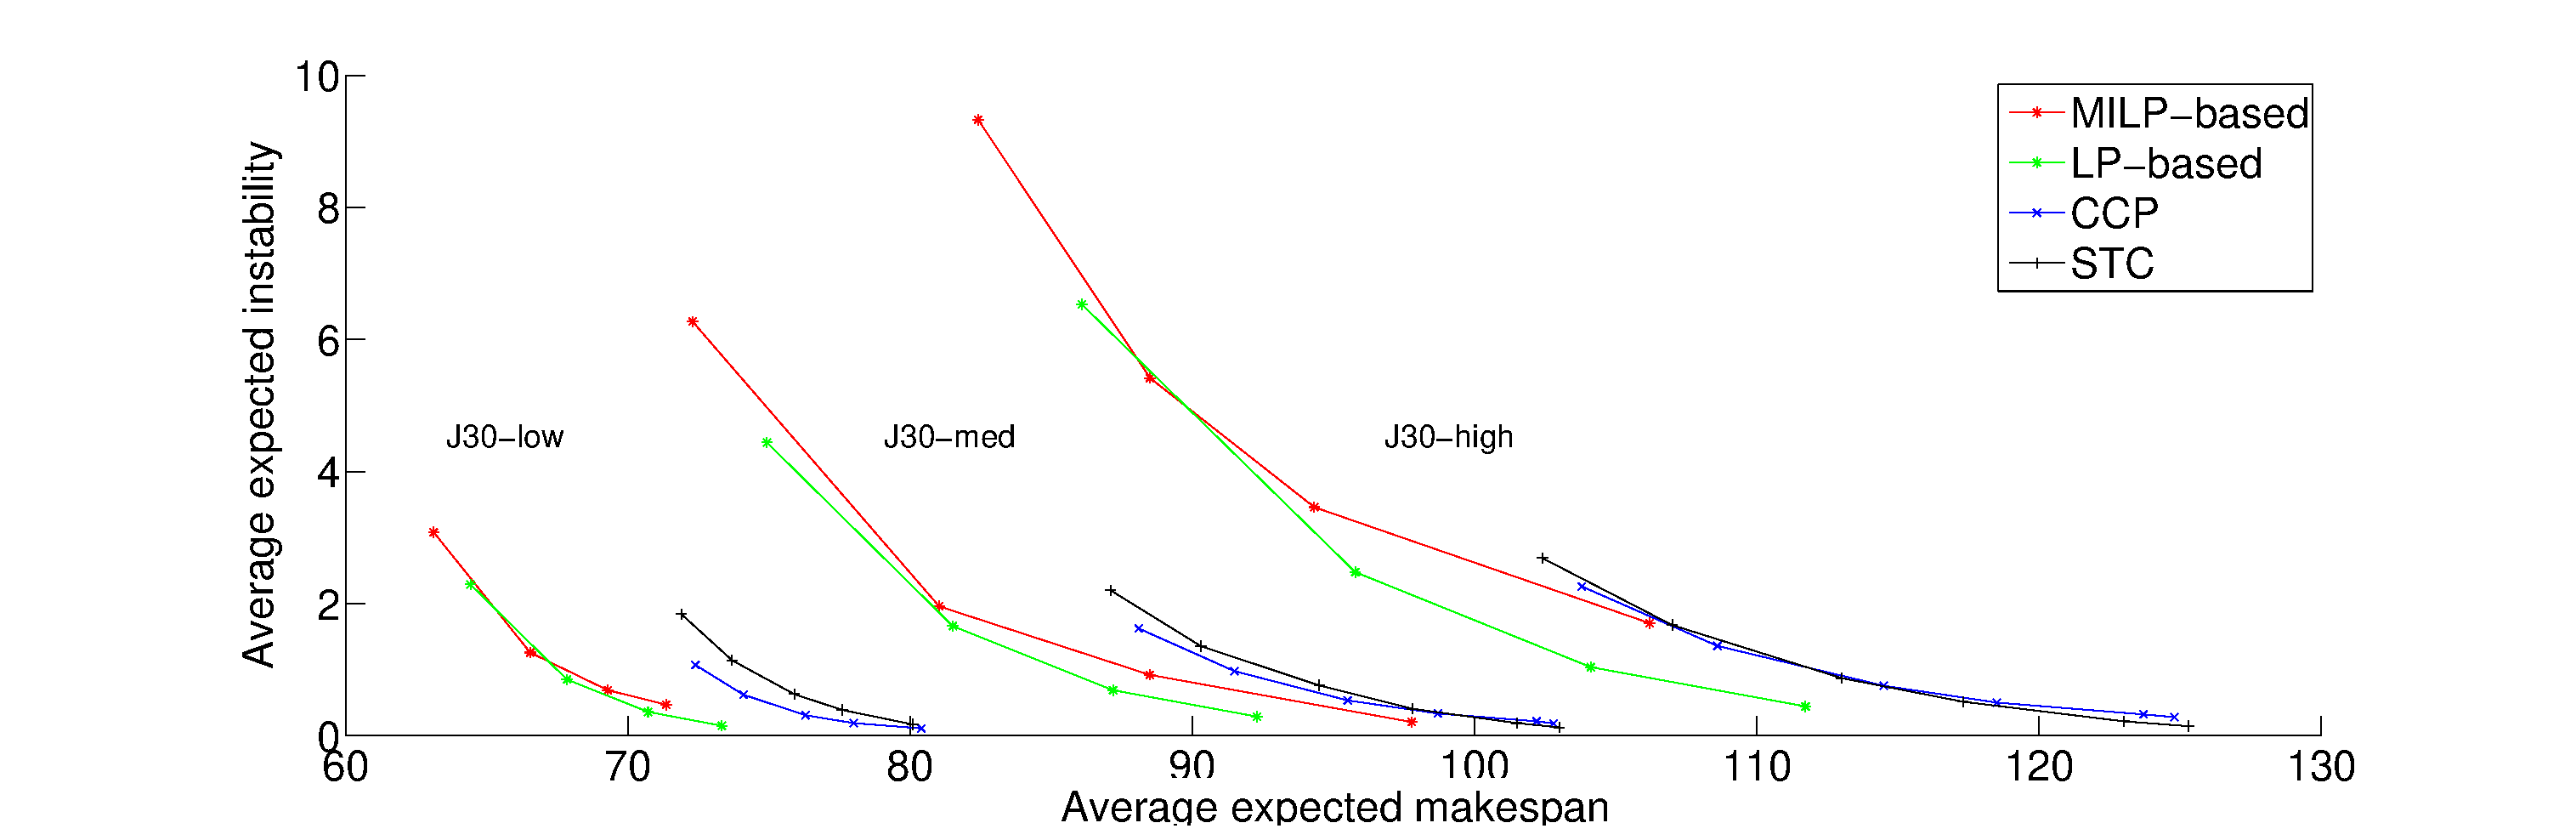
\includegraphics[width=1.0\textwidth]{chapter/mista-stability/figure1.eps}
 		\caption{Trading expected makespan for stability.}
 		\label{fig-experiments-1}
 	\end{figure}
 	
  	\begin{figure} 
 		\centering  
   		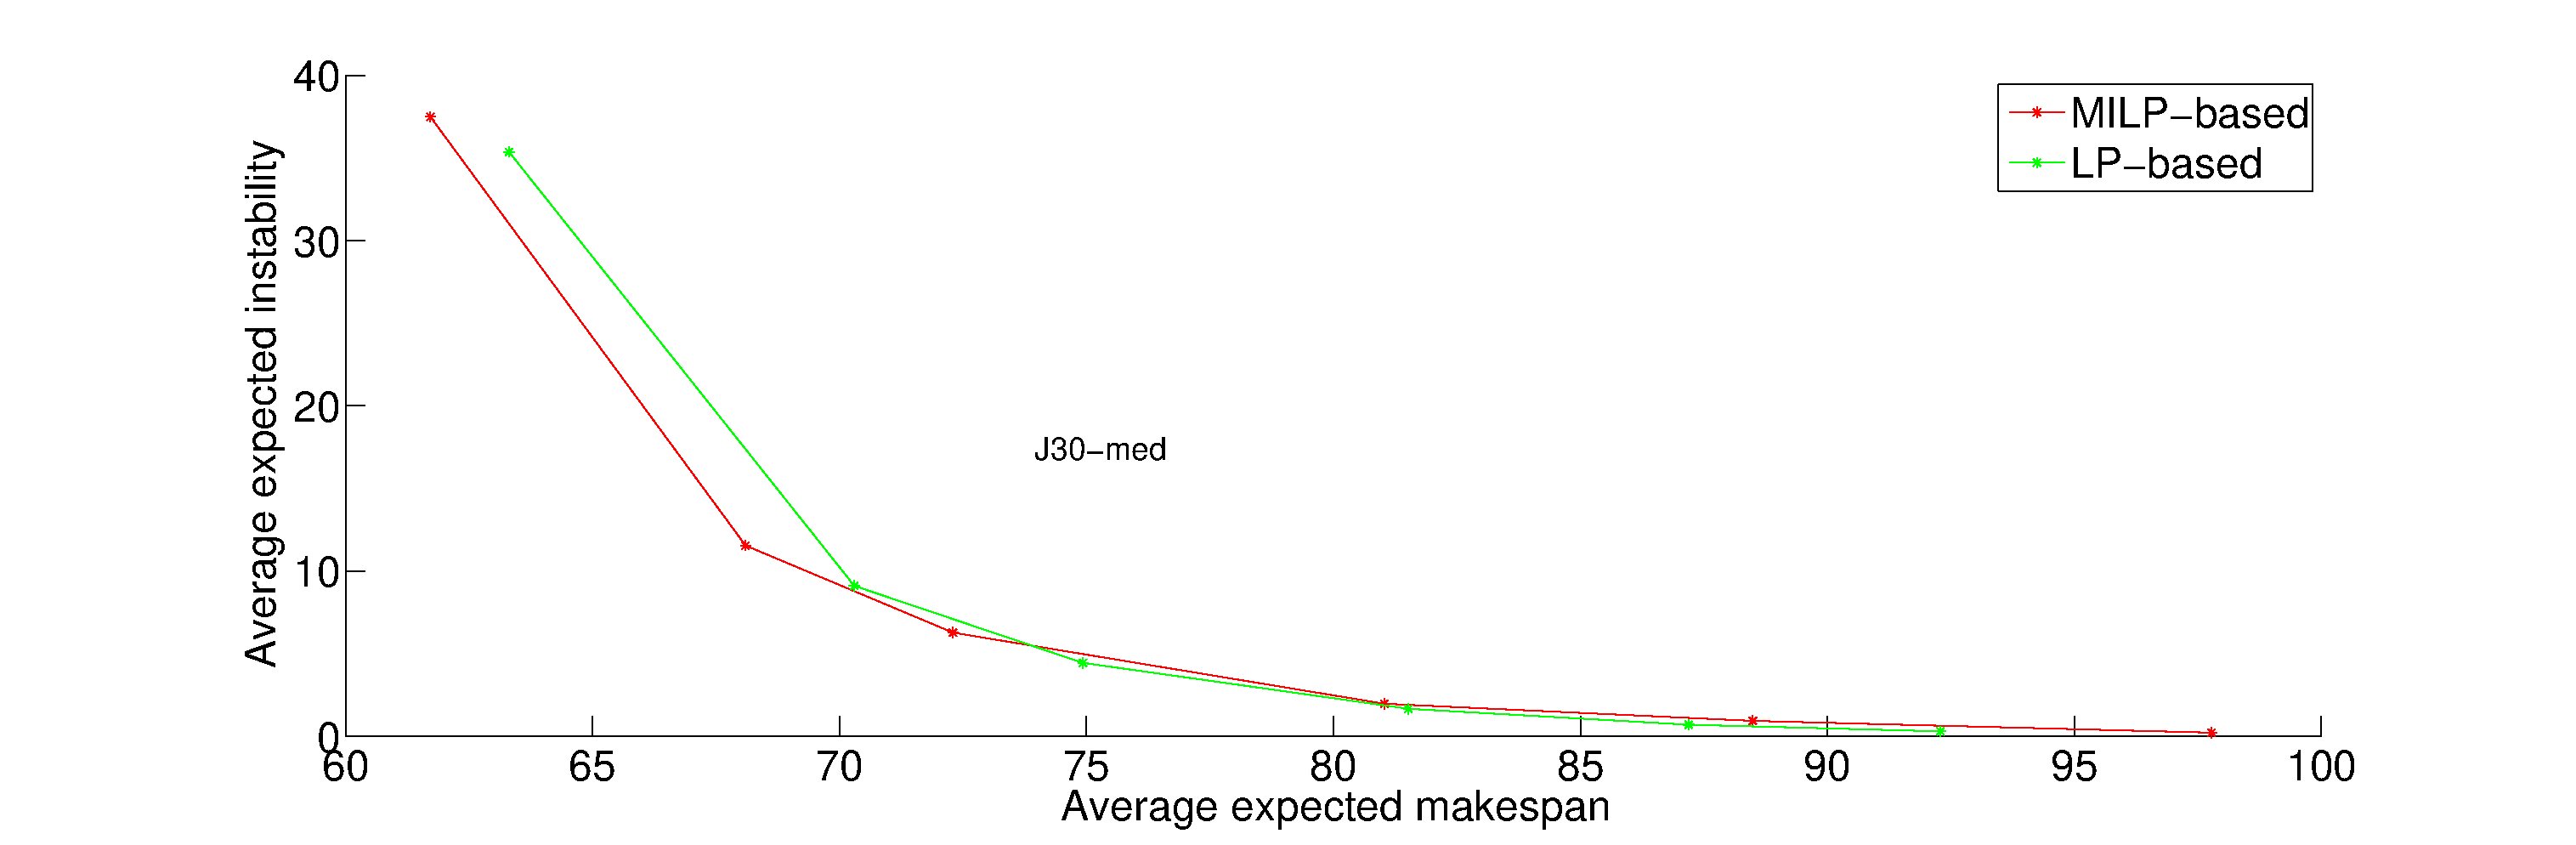
\includegraphics[width=1.0\textwidth]{chapter/mista-stability/figure2.eps}
 		\caption{Trading expected makespan for stability for higher $\alpha$.}
 		\label{fig-experiments-2}
 	\end{figure}
 	
 	In Figure~\ref{fig-experiments-1},
 	the data-points for each method are displayed as a tradeoff curve, 
 	on each of the three bench-sets, resulting in three "clusters" of tradeoff curves.
 	A tradeoff curve captures the average performance of the method on that bench-set.
 	Specifically, each data-point is two-dimensional and records the average expected makespan and average 
 	expected instability for a certain choice of the tradeoff parameter(s),
 	where the average is taken over all 480 instances of the bench-set.
  	Data-points for CCP and STC are borrowed
 	from the work of Vilches and Demeulemeester \cite{lamas2015}.	
  	Data-points for our heuristics are obtained by setting $\alpha=0.05$, $0.1$, $0.2$, and $0.4$.
 	Higher alpha values correspond to data-points closer to the upper left corner,
 	with higher instability and lower makespan.	
 	
 	Figure~\ref{fig-experiments-2} focuses on the medium variability case for higher $\alpha$ values,
 	including additional data-points for $\alpha=0.6$ and $\alpha=0.9$.
 	This allows us to compare the MILP-based and LP-based heuristics when
 	more emphasis is put on minimizing expected makespan.
 	
 	The expected makespan and expected instability of the solution
 	provided by each of the methods on a particular instance
 	is computed with a sample $\Gamma^{large} \subset \mathbb{R}^n$ 
 	comprising $|\Gamma^{large}| = 10^3$ realization of durations vector $\xD$.
 	Note that the data-points of Vilches and Demeulemeester were computed with a different sample of size $10^3$.
 	We assume that $10^3$ is a sufficiently large sample size to facilitate comparability with our results.
 	
 	\paragraph{Configuration of heuristics.}
 	The sample $\Gamma^{milp}$ used by our MILP-based heuristic during optimization
 	(see line 6 of Algorithm~\ref{alg-milp-heuristic}) is of size $|\Gamma^{milp}| = 30$.
 	Our MILP-based heuristic is configured to perform three (3) iterations and
 	the number of highly critical arcs removed in each iteration 
 	(see line 5 of Algorithm~\ref{alg-milp-heuristic}) is $|\mathcal{H}| = 20$.
 	Note that the criticality of the arcs is computed based on sample $\Gamma^{large}$
 	(this is done efficiently, in time quadratic in $n$ and linear in $|\Gamma^{large}|$).
  	The solver we use is \textsc{CPLEX} version 12.6.
  	Furthermore, we set a time-limit for the solver to 50 seconds
  	(since each iteration starts from a feasible solution, 
  	the solver will always return with a solution within the time-limit).
  	The polynomial-time complexity of our LP-based heuristic (no binary variables in the model)
  	allows us to use a large sample during optimization.
  	In fact, we use sample $\Gamma^{large}$.
  	To find a deterministic schedule (as required in step 1 of this LP-based heuristic)
  	we used a priority rule procedure recently proposed in \cite{de2014novel}.
  	Vilches and Demeulemeester use a sample of size $10^2$ during optimization, for both STC and CCP.
  	Furthermore, they limit the time spent in solving their 
  	CCP model on an instance to a maximum of 10 seconds. 
 
   	
  	\paragraph{Observations.}
  	Figure~\ref{fig-experiments-1} suggests that
   	regardless of the mode of variability (low, medium, or high),
  	when the purpose is to achieve near-zero instability,
  	the LP-based heuristic yields the best results.
  	This can be attributed to the efficiency of solving a LP model,
  	which enables us to use a large sample (of size $10^3$ in this case) during optimization.
  	
  	Figure~\ref{fig-experiments-2} suggests that
  	even though the sample used during optimization is much smaller
  	for the MILP-based heuristic (of size $30$),
  	it is more effective than the LP-based heuristic for higher $\alpha$ values
  	(i.e. when minimizing instability is  more important than minimizing makespan).
  	Both the LP-based and the MILP-based heuristics start from the same es-policy
  	(see step 1 in section~\ref{sec-lp} and line 2 of Algorithm~\ref{alg-milp-heuristic}, respectively).
  	However, the MILP-based heuristic restructures the policy and this enables
  	it to perform better at minimizing expected makespan.
  	
  	Restructuring the policy comes at the cost of efficiency.
   	With three iterations allowed per instance,
  	this yields an average of 50 seconds per instance for the MILP-based heuristic.
  	The LP-based heuristic is considerably more efficient, with an average of 1.5 seconds per instance.
  	Vilches and Demeulemeester report that STC spends on average 0.2 seconds per instance,
  	while their CCP approach spends on average 10 seconds per instance. 
 	

\section{Conclusions and future work}
\label{sec-conclusion}

This paper proposes the PS-RCPSP problem model which,
assuming stochastic activity durations,
asks to find a so-called earliest-start (es) policy and
a proactive schedule that together minimize the weighted 
sum of expected project makespan and expected instability.
Extending an existing MILP model for the RCPSP,
a MILP model for PS-RCPSP is presented, which allows us to 
find optimal (es-policy, proactive schedule) pairs.
Solving this problem to optimality might require an impractical amount of time,
even for instances with few activities (e.g. 30).
Therefore, we propose a LP-based and a MILP-based heuristic for the PS-RCPSP.
Our LP-based heuristic optimizes the proactive schedule by keeping the es-policy part of the  solution fixed.
Our MILP-based heuristic optimizes the structure of the policy together with the proactive schedule.
The LP-based heuristic, which is rather efficient, seems to be more effective compared to the state-of-art
(i.e. achieves smaller expected makespan for a certain level of expected instability) especially
when the aim is to achieve close to zero instability.
The MILP-based heuristic is rather effective when the aim is to
achieve low expected makespan at the cost of moderate or high instability.
In contrast to existing state-of-art approaches such as
CCP \cite{lamas2015} and STC \cite{van2008},
our heuristics rely on the idea of optimizing 
the proactive schedule together with the scheduling policy.
This difference might in part explain observed performance differences.

Future work involves a thorough experimental analysis of the proposed heuristics,
not for the purpose of comparing them to the state-of-art,
but for a deeper understanding of their behavior and its
dependence on problem characteristics.
Furthermore, most existing stochastic project scheduling works are evaluated on instances where
the deterministic RCPSP counterpart instance 
(formed by mean activity durations) serves as a good approximation of the stochastic instance.
This is exploited by our heuristics and other heuristics such as STC.
However, in certain practical domains (e.g. maintenance scheduling),
the duration of some activities is known a-priori with accuracy,
while the duration of other activities follows a distribution with very high variance.
In maintenance scheduling, for example, "inspection" activities have known durations
but "repair" activities might be (un)necessary with certain probabilities. 
We would like to investigate performance on such instances 
which cannot be approximated well by their determinitic counterpart.
%
%\begin{acknowledgements}
%We would like to thank our anonymous reviewers for their constructive remarks.
%This research belongs to the \emph{Job Scheduling Problem} part of the 
%\emph{Rolling Stock Life Cycle Logistics} applied research and development programme, 
%funded by \emph{NS/NedTrain}.
%\end{acknowledgements}
%
%% BibTeX users please use one of
%\bibliographystyle{plain}      % basic style, author-year citations
%%\bibliographystyle{spmpsci}      % mathematics and physical sciences
%%\bibliographystyle{spphys}       % APS-like style for physics
%\bibliography{p}   % name your BibTeX data base
%
%% Non-BibTeX users please use
%%\begin{thebibliography}{}
%%
%% and use \bibitem to create references. Consult the Instructions
%% for authors for reference list style.
%%
%%\bibitem{RefJ}
%% Format for Journal Reference
%%Author, Article title, Journal, Volume, page numbers (year)
%% Format for books
%%\bibitem{RefB}
%%Author, Book title, page numbers. Publisher, place (year)
%% etc
%%\end{thebibliography}
%
%\end{document}
%% end of file sample.tex
%
%


\chapter[Stable dispatching via dynamic programming]{Stable dispatching via dynamic programming\protect\footnotemark{}\protect\footnotetext{
This chapter has been published as:
K.S. Mountakis, T.B. Klos and C. Witteveen. Stochastic Task Networks: Trading Performance for Stability. 
In \emph{International Conference on AI and OR Techniques in Constraint Programming for Combinatorial Optimization Problems (CPAIOR)}, pages 302-311, 2017.}}
\label{chapter/cpaior-stability}
%\documentclass{llncs}
%
%% included packages
%\usepackage{amsmath}
%\usepackage{amsfonts}
%\usepackage{microtype}
%\usepackage{algorithm}
%\usepackage{algorithmic}
%\usepackage{subcaption}
%\captionsetup{compatibility=false}
%\usepackage{microtype}
%\usepackage{tikz}
%\usetikzlibrary{arrows,automata}
%\usetikzlibrary{arrows.meta}
%
%\usetikzlibrary{external}
%%\tikzexternalize
%
%
%\makeatletter
%\newcommand{\@chapapp}{\relax}%
%\makeatother
%%\usepackage[title,toc,titletoc,header]{appendix}
%
%% custom commands
%\newcommand{\z}[1]{\mathcal{#1}}
%\newcommand{\comm}[1]{\vspace{0.2cm}\framebox{#1}\vspace{0.2cm}}
%
%\newtheorem{gap}{Gap}
%\newtheorem{lemm}{Lemma}
%\newtheorem{exmp}{Example}
%\newtheorem{defn}{Definition}
%\newtheorem{obsv}{Observation}
%
%\begin{document}
%
%\pagestyle{headings}  % switches on printing of running heads
%%\addtocmark{} % additional mark in the TOC
%%\tableofcontents
%
%\mainmatter              % start of the contributions
%
%\title{Stochastic Task Networks}
%\subtitle{Trading performance for stability}
%
%\titlerunning{Stable Stochastic Activity Networks}  
%% abbreviated title (for running head) 
%
%\author{Kiriakos Simon Mountakis \inst{1} \and Tomas Klos \inst{2} \and Cees Witteveen\inst{1}}
%\authorrunning{Mountakis et al.} 
%\institute{Delft University of Technology, Delft, The Netherlands \and
%Utrecht University, Utrecht, The Netherlands}
%
%\maketitle          
%
%\begin{abstract}
%	This paper addresses a problem of practical value in project scheduling:
trading expected makespan for stability,
under stochastic activity duration uncertainty.
We present the formal statement of a problem 
that we name Proactive Stochastic RCPSP (PS-RCPSP).
Assuming activity durations follow known probability distributions,
PS-RCPSP asks to find a so-called earliest-start (es) policy and
a proactive schedule that together minimize the weighted 
sum of expected project makespan and expected instability
(deviation of the realized from the proactive schedule).
%
Extending an existing MILP model for the well-known deterministic 
Resource-Constrained Project Scheduling Problem (RCPSP),
we present a MILP model for PS-RCPSP, which allows us to 
find optimal (es-policy, proactive schedule) pairs.
To deal with instances of practical size,
we propose a Linear Programming (LP)-based 
and a Mixed-Integer LP (MILP)-based heuristic.
Our LP-based heuristic optimizes the proactive schedule while 
keeping the es-policy part of the solution fixed.
Our MILP-based heuristic aims to optimize the structure of the policy together with the proactive schedule.
In contrast to existing state-of-art approaches such as
CCP \cite{lamas2014purely} and STC \cite{van2008},
our heuristics rely on optimizing the proactive schedule together with the scheduling policy.
%
Experiments show that the LP-based heuristic is efficient and compares favorably with the state-of-art 
(i.e.\ achieves smaller expected makespan for a certain level of expected instability)
when the aim is to achieve near-zero instability at the cost of higher makespan.
The MILP-based heuristic seems more effective (albeit not as efficient) when the aim is to
achieve low expected makespan at the cost of moderate or high instability.

%	\keywords{activity network, stochastic scheduling, solution robustness}
%\end{abstract}
%
\section{Introduction}

A \emph{stochastic task network} is a directed acyclic graph $G(V, E)$ 
with each node in $V = \{1,\ldots,n\}$ representing a task with a random duration and 
each arc $(i,j)\in E$ representing a precedence-constraint between tasks $i$ and $j$,
specifying that task $j$ cannot start unless task $i$ has finished.
%
Such networks appear in several domains like project scheduling \cite{leus2011resource}, 
parallel computing \cite{shestak2008}, or even digital circuit design \cite{blaauw2008},
where there is a need to model a partial order of events with uncertain durations.
%
Postulating that a model of uncertainty is known, 
task durations are described by a random vector $D=(D_1,\ldots,D_n)$ with a known probability distribution.
%
In project scheduling, for example, the duration $D_i$ of task $i$ may turn out to be shorter or longer 
than a nominal value according to a certain distribution.
%In digital circuit design, a task $i$ corresponds to a gate with an input/output delay $D_i$ that 
%varies with a certain distribution across gates due to manufacturing imperfections.

A given task network is typically mapped to a \emph{realized schedule} (i.e. an assignment of start-times to tasks) via \emph{earliest-start dispatching};
i.e. observing outcome durations and starting a task immediately when precedence-constraints allow 
(i.e. not later than the maximum finish-time of its network predecessors).
Random durations make the realized start-time of a task (and the overall realized schedule makespan) also random.
Since \emph{PERT networks} \cite{malcolm1959}, 
a large body of literature focused on the problem of determining the makespan distribution \cite{adlakha1989},
eventually shown to be a hard problem \cite{hagstrom1990}. 
A variety of efficient heuristics have been developed so far (see \cite{blaauw2008}), 
among which Monte Carlo sampling remains, perhaps, the most practical.

Consider, for example, the stochastic task network in Fig.~\ref{fig-house}, 
detailing the plan of a house construction project,
assuming task durations are random variables that follow the uniform distribution within respective intervals.
With earliest-start dispatching, the overall duration of the project (i.e. the realized schedule makespan) 
will range between 12 and 20 days with an expected value of a little over 16 days.


\begin{figure}[!t]
	\centering
	\begin{subfigure}[b]{0.45\textwidth}
		\begin{tikzpicture}
			\begin{scope}[every node/.style={circle,thin,draw}]
 				\node (1) at (0,+0)	{\scriptsize 1};
				\node (2) at (1.2,-1)	{\scriptsize 2};
				\node (3) at (1.2,+1)	{\scriptsize 3};
				\node (4) at (2.4,-1)	{\scriptsize 4};
				\node (5) at (3.5,+1)	{\scriptsize 5};
				\node (6) at (2.4,-0)	{\scriptsize 6};
				\node (7) at (3.5,-1)	{\scriptsize 7};
				\node (8) at (4.5,+0)	{\scriptsize 8};
			\end{scope}

			\begin{scope}[>={Stealth[black]},
				every node/.style={fill=white,circle},
				every edge/.style={draw=black,thin}]
				\path [->] (1) edge (2);				
				\path [->] (1) edge (3);				
				\path [->] (2) edge (4);				
				\path [->] (3) edge (5);				
				\path [->] (3) edge (6);				
				\path [->] (4) edge (7);				
				\path [->] (5) edge (8);				
				\path [->] (6) edge (7);				
				\path [->] (7) edge (8);				
 			\end{scope}
		\end{tikzpicture}
		\subcaption{Example construction plan.}
		\label{fig-house-a}
	\end{subfigure}
	~
	\begin{subfigure}[b]{0.4\textwidth}
		\begin{center}
		    \begin{tabular}{ l l c }
			    & Tasks & Durations (days) \\ \hline
			    1. & Erect walls & 2-4  \\ 
			    2. & Finish walls & 3-5 \\ 
			    3. & Finish roof & 2-6 \\
			    4. & Install plumbing & 3-5 \\
			    5. & Finish exterior & 6-8 \\
			    6. & Install electricity & 3-5 \\
			    7. & Paint interior & 2-4 \\
			    8. & Finishing touches & 1-1 \\
		    \hline
		    \end{tabular}
		\end{center}
	\subcaption{Estimated task durations.}
	\label{fig-house-b}
	\end{subfigure}
	\caption{A motivating example.}
	\label{fig-house}
\end{figure}


This paper addresses a problem which, to our knowledge, has not been addressed in existing literature.
To motivate our problem, let us return to the earlier example and suppose task 7 
(``Paint interior'') is assigned to a painting crew charging \$100 per day.
Assume we are willing to hire them for at least 4 days (the maximum number of days they will need) and for at most 6 days; i.e. we have a budget of \$600 for painting.
With earliest-start dispatching, 7 may start within 8 to 15 days from the project start (the start-date of task 1).
A challenge that arises in this situation is deciding when to hire the painting crew,
because to allow for an expected makespan of a little over 16 days (as mentioned earlier),
we must book the painting crew from the 8-th day and until the 19-th day, at the excessive cost of \$1100.
% ... est requires an agile availability of resources that might be too costly
The solution we examine here, is to use a different dispatching strategy,
associating task 7 with a \emph{planned release-time}, $t_7$, 
before which it may not start even if installing plumbing and electricity are finished earlier than $t_7$.
If we choose that 7 may not start earlier than, e.g., $t_7 = 13$ days from the project start,
we only need to book the painting crew on the 13-th day until the 19-th day, for an acceptable cost of \$600.
However, the price to pay for this stability is an expected makespan increase to a little over 17 days.

Now suppose that after assessing our budget carefully it turns out that each task may deviate at most, say $w$ days, from its respective planned release-time.
The emerging question addressed in this paper is:
\begin{quote}
	Which planned release-times reach the desired level of stability\footnote{As in Bidot et al. \cite{bidot2009}, stability here refers to the extent that a predictive schedule (planned release-times in our case) is expected to remain close to the realized schedule.}
	while minimizing the incurred performance penalty?
\end{quote}

This problem does not involve resource-constraints.
However, task networks are often used in the area of resource-constrained scheduling under uncertainty (see \cite{beck2002,herroelen2005})
to represent solutions (e.g. the \emph{earliest-start policy} \cite{igelmund1983}, the \emph{partial-order schedule} \cite{policella2004,godard2005,bonfietti2014}).
Thus, our work is expected to be useful in dealing with associated problems,
such as distributing slack in a resource-feasible schedule to make it insensitive to durational variability \cite{davenport2014}.

\subsubsection*{Organization}
A formal problem statement and its LP formulation are presented in Section~2. 
As the resulting LP can be quite costly to solve,
Section~3 presents our main result, an efficient dynamic programming algorithm.
Section~4 concludes the paper and outlines issues to be addressed in future work.



\section{Problem definition}
We are given a task network $G(V,E)$ and a stochastic vector $D=(D_1,\ldots,D_n)$ describing task durations.
Let $\z{Q}$ index the space of all possible realization scenarios for $D$ such that $d_{ip}$ denotes the realized duration of task $i$ in scenario $p\in\z{Q}$.
We assume to know the probability distribution of $D$; i.e. the probability $\mathbb{P}[D = (d_{1p},\ldots,d_{np})]$ for all $p\in \z{Q}$.
To limit the unpredictability of the realized schedule, we want to associate tasks with respective 
\emph{planned release-times} $t=(t_1,\ldots,t_n)$ such that the realized schedule is formed by starting a task 
as early as permitted by precedence-constraints, but not earlier than its release-time.
That is, the start-time $s_{jp}$ of task $j$ in scenario $p$ will be determined as:
\begin{align}
	s_{jp} = \max[\max_{(i,j)\in E} (s_{ip} + d_{ip}), t_j] \label{sj-est}
\end{align}

Given a sample $\z{P} \subseteq \z{Q}$ of size $m$ of the stochastic durations vector,
this paper is devoted to the following problem:
\begin{align}
	\tag{$P$}
	\min_{t\geq 0} \quad 	& F := \sum_{j\in V, p\in\z{P}} s_{jp} 				&	\\
	\textrm{subject to} \quad 	& s_{jp} = \max[\max_{(i,j)\in E} (s_i + d_i), t_j]		& \forall j\in V, p\in \z{P} 
	\label{P-sj-compact} \\
				& s_{jp} - t_j \leq w 						& \forall j\in V, p\in \z{P}
\end{align}
This problem tries to optimize a trade-off between stability and performance:
release-times are sparsely spread in time in order to form a stable schedule, 
i.e. such that in every considered scenario a realized start-time will stay within $w$ time-units  from the corresponding release-time.

Since the whole space of possible duration realizations, $\z{Q}$, may be too large, or even infinite,
we only consider a manageable sample $\z{P} \subseteq \z{Q}$ during optimization.%
\footnote{Knowing the distribution of $D$, we assume to be able to draw $\z{P}$.}%
At the same time, we want to ensure a minimal performance penalty $F - F^*$ where $F^*$ denotes the throughput of earliest-start dispatching with no release-times.
\footnote{The reader can easily recognize the similarity of the proposed LP with a so-called Sample Average Approximation (SAA)
of a stochastic optimization problem \cite{kleywegt2002}.}

Instead of minimizing a standard performance criterion like expected makespan,
we choose to maximize \emph{expected throughput}, $\frac{1}{m} \frac{n}{\sum_{j,p} s_{jp}}$,
which equals the average rate at which tasks finish over all scenarios.
It can be shown that a schedule of maximum throughput is one of minimum makespan and/or tardiness 
(in case tasks are associated with deadlines).
We maximize throughput indirectly by minimizing its inverse,
with the constant $\frac{m}{n}$ omitted for simplicity.

\subsubsection{LP formulation}
The resulting problem is not easy to handle due to the equality constraint, 
but using a standard trick it can be rewritten as the following linear program (LP):
\begin{align}
	\tag{$P$}
	\min_{s,t\geq 0} \quad	&	F := \sum_{j\in V, p\in\z{P}} s_{jp} 				&	\\
	\textrm{subject to}\quad	&	s_{jp} \geq s_{ip} + d_{ip} 		& (i,j) \in E, p \in \z{P} \label{P-sisj} \\
				&	s_{jp} \geq t_j 			& j \in V, p \in \z{P}\label{P-tjsj} \\
				&	s_{jp} - t_j \leq w 			& j \in V, p \in \z{P}\label{P-sjtj}
\end{align}
Note that the solution-space of the resulting LP encompasses that of the original formulation.
However, it is easy to show that both problems have the same set of optimal solutions,
because a solution $(s,t)$ for the LP cannot be optimal unless it satisfies (\ref{P-sj-compact}).

Currently, the best (interior-point) LP solvers have a complexity of $O(N^3M)$ where $N$ is the number of variables and 
$M$ the input complexity \cite{potra2000}.
Thus, letting $\delta \leq n$ denote the max in-degree in $G(V, E)$,
the cost of solving $(P)$ as an LP with $n m$ variables and $O(n \delta m)$ constraints can be bounded by $O(n^4 m^4 \delta) \subseteq O(n^5 m^4)$,
which can be daunting even for small instances.
Fortunately, as shown in the following section, 
we manage to obtain the substantially tighter bound of $O(n^2 m)$ for solving $(P)$,
by exploiting its simple structure to devise a dynamic programming algorithm.


\section{Fast computation of planned release-times}
We first show that a fixed relationship between variables $s_{jp}$ and $t_j$
can be assumed while looking for an optimal $(s,t)$.
Based on this, a problem $(P')$ is defined which can be solved instead of $(P)$.

\subsubsection{A tighter formulation}
Begin by rewriting (\ref{P-sjtj}) as $t_j \geq \max_p s_{jp} -w \,, \forall j \in V$.
Now, let $\Lambda$ denote the set of all feasible $(s,t)$ for problem $(P)$ and 
let $\Lambda^* \subseteq \Lambda$ be that part of the solution-space that 
only contains $(s,t)$ for which $t_j = \max_p s_{jp} - w$ for all $j$.

\begin{lemm}
	\label{lemm-Lambda}
	For every feasible $(s,t) \in \Lambda \setminus \Lambda^*$ 
	there exists $(s',t') \in \Lambda^*$ with equal objective value.
\begin{proof}
	Consider feasible $(s,t)$ with
 	$t_j = \max_p s_{j^*p} - w + c$ with  $c > 0$ for some $j^*$.
	Construct $t'$ by letting $t'_j = t_j$ for all $j \neq j^*$ and $t'_{j^*} = t_{j^*} - c = \max_p s_{j^*p} - w$.
	Trivially, if $(s,t)$ is feasible, so is $(s, t')$, with the same objective value.
	Keeping $s$ fixed, we may repeat this construction to enforce that $t_j = \max_p s_{jp} - w$ for all $j$
	and have $(s, t') \in \Lambda^*$.
\end{proof}
\end{lemm}

The previous result allows us to consider the following problem, 
obtained by substituting $\max_{p'\in \z{P}} s_{jp'} - w$ for $t_j$ in $(P)$:
\begin{align}
	\tag{$P'$}
	\min_{s\geq 0} \quad	&	\sum_p s_{np} 								& \\
	\textrm{subject to}\quad	&	s_{jp} \geq s_{ip} + d_{ip}							& (i,j) \in E, p \in \z{P} \label{P'-sisj} \\
				&	s_{jp} \geq \max_{p'\in \z{P}} s_{jp'} - w			& j \in V, p \in \z{P}\label{P'-tjsj} \\
				&	s_{jp} - (\max_{p'\in \z{P}} s_{jp'} -w)  \leq w 	& j \in V, p \in \z{P}\label{P'-sjtj}
\end{align}
Clearly, $(s,t) \in \Lambda^*$ iff $s$ is feasible for $(P')$.%
\footnote{Since  $(s,t)\in \Lambda^*$ implies  $\max_{p'} s_{jp'} - w = t_j$ for all $j$.} 
In other words, the solution-space of $P'$ comprises only those $s$ that can be paired with $t$ by letting $t_j = \max_p s_{jp} - w$
to form a feasible $(s,t)$ for $(P)$.
By Lemma~\ref{lemm-Lambda}, if $s$ is optimal for $(P')$, then $(s,t)$ is optimal for $(P)$.
Also, if $(P)$ has a solution (i.e. if $G(V,E)$ is acyclic),then $(P')$ also has a solution.


\subsubsection{The resulting STP}
Formulation $(P')$ is useful because it can be cast as a certain type of 
Temporal Constraint Satisfaction Problem (TCSP) \cite{dechter1991}.
We start by noting that (\ref{P'-sjtj}) is always true and can be omitted.
Moreover, (\ref{P'-tjsj}) can be rewritten as (\ref{P'-pp}), 
to obtain the following reformulation:
\begin{align}
	\tag{$P'$}
	\min_{s\geq 0} \quad 	&	\sum_p s_{np} 			& \\
	\textrm{subject to} \quad	&	s_{ip} - s_{jp}  \leq -d_{ip}		& (i,j) \in E, p \in \z{P} \label{P'-sisj} \\
				&	s_{jp} - s_{jp'} \leq w			& (p, p') \in \z{P}^2, j \in V \label{P'-pp}
\end{align}

Constraints (\ref{P'-sisj}) and (\ref{P'-pp}) effectively represent the solution-space of a 
Simple Temporal Problem (STP)  \cite{dechter1991} with temporal variables $\{s_{jp}: j\in V, p\in \z{P}\}$.
The structure of the resulting STP (specifically, of its \emph{distance graph} \cite{dechter1991}) is demonstrated in Fig.~\ref{fig-STP}.

\begin{figure}
	\centering
		\begin{subfigure}[b]{0.4\textwidth}
		\begin{tikzpicture}
			\begin{scope}[every node/.style={circle,thin,draw}]
				\node (1a) at (+0+0,+0+0)	{\scriptsize $1$};
				\node (2a) at (+2+0,+1+0)	{\scriptsize $2$};
				\node (3a) at (+2+0,-1+0)	{\scriptsize $3$};
				\node (4a) at (+4+0,-0+0)	{\scriptsize $4$};
				
			\end{scope}

			\begin{scope}[>={stealth[black]},
				every node/.style={fill=white,circle},
				every edge/.style={draw=black,thin}]
				\path [->] (1a) edge node {\tiny $D_{1}$} (2a);
				\path [->] (1a) edge node {\tiny $D_{1}$} (3a);
				\path [->] (2a) edge node {\tiny $D_{2}$} (4a);
				\path [->] (3a) edge node {\tiny $D_{3}$} (4a);			
 			\end{scope}
		\end{tikzpicture}
		\subcaption{}
		\label{fig-STN}
	\end{subfigure}
	~
	\begin{subfigure}[b]{0.4\textwidth}
\begin{tikzpicture}
			\begin{scope}[->,>=stealth',shorten >=1pt,auto,
                semithick, scale = 1, transform shape,
                every node/.style={circle,thin,draw}]
				\node (z) at (-1.5,+1.5)	{\scriptsize $z$};
				
				\node (1a) at (+0+0,+0+0)	{\scriptsize $s_{1p}$};
				\node (2a) at (+2+0,+1+0)	{\scriptsize $s_{2p}$};
				\node (3a) at (+2+0,-1+0)	{\scriptsize $s_{3p}$};
				\node (4a) at (+4+0,-0+0)	{\scriptsize $s_{4p}$};
				
				\node (1b) at (+0+0.0,+0+3.0)	{\scriptsize $s_{1p'}$};
				\node (2b) at (+2+0.0,+1+3.0)	{\scriptsize $s_{2p'}$};
				\node (3b) at (+2+0.0,-1+3.0)	{\scriptsize $s_{3p'}$};
				\node (4b) at (+4+0.0,-0+3.0)	{\scriptsize $s_{4p'}$};				
			\end{scope}

			\begin{scope}[>={stealth[black]},
				every node/.style={fill=white,circle},
				every edge/.style={draw=black,thin}]
				
				% z1 arcs
				\path [<-] (z) edge[bend right=15] node {\tiny $0$} (1a);
				\path [->] (z) edge[bend left=15] node {\tiny $0$} (1a);
				\path [<-] (z) edge[bend right=15] node {\tiny $0$} (1b);
				\path [->] (z) edge[bend left=15] node {\tiny $0$} (1b);	
						
				% ij arcs for scenario p
				\path [<-] (1a) edge node {\tiny $-d_{1p}$} (2a);
				\path [<-] (1a) edge node {\tiny $-d_{1p}$} (3a);
				\path [<-] (2a) edge node {\tiny $-d_{2p}$} (4a);
				\path [<-] (3a) edge node {\tiny $-d_{3p}$} (4a);
				
				% ij arcs for scenario p'
				\path [<-] (1b) edge node {\tiny $-d_{1p'}$} (2b);
				\path [<-] (1b) edge node {\tiny $-d_{1p'}$} (3b);
				\path [<-] (2b) edge node {\tiny $-d_{2p'}$} (4b);
				\path [<-] (3b) edge node {\tiny $-d_{3p'}$} (4b);	

							
				% s1p - w - s1p'
				\path [->] (1a) edge[bend right=8] node[] {\tiny $w$} (1b);
				\path [<-] (1a) edge[bend left=8] node[] {\tiny $w$} (1b);
				
				% s2p - w - s2p'
				\path [dotted,<->] (2a) edge[bend left=15] node[pos=0.7] {\tiny $w$} (2b);
				
				% s3p - w - s3p'
				\path [dotted,<->] (3a) edge[bend right=15] node[pos=0.3] {\tiny $w$} (3b);
				
				% s4p - w - s4p'
				\path [->] (4a) edge[bend right=8] node[] {\tiny $w$} (4b);
				\path [<-] (4a) edge[bend left=8] node[] {\tiny $w$} (4b);
			\end{scope}
		\end{tikzpicture}
		\subcaption{}
		\label{fig-STN}
	\end{subfigure}

	\caption{Example task network (a) and resulting STP (b) for a sample $P=\{p, p''\}$.}
	\label{fig-STP}
\end{figure}

The \emph{earliest start time} (est) solution of any given STP (assuming it is consistent)
assigns to each variable the smallest value it may take over the set of feasible solutions.
Therefore,  the est solution of the resulting STP optimally solves $(P')$, leading us to the following observation.

\begin{obsv}
	By Lemma~\ref{lemm-Lambda}, an optimal solution $(s,t)$ for $(P)$ can be formed by finding the 
	earliest start time solution $s$ of the resulting STP and pairing it with $t$ formed by letting 
	$t_j = \max_{p\in \z{P}} s_{jp} - w$ for all $j$.
\end{obsv}

The est value of $s_{jp}$ is the length of the shortest-path (in the distance graph)
from (the node corresponding to) $s_{jp}$ to the special-purpose variable $z$ which is fixed to zero.
Those values can be found with a single-source shortest-path algorithm (e.g. Bellman-Ford \cite{pallottino1984})
in time $O(N M)$ where $N$ is the number of nodes and $M$ the number of arcs. 
In our case, $N=n m$ and $M = O(nm\delta)$, yielding $O(n^3m^2)$; already a better bound than that of solving $(P)$ as an LP.
However, in the following we obtain an even better bound with a dynamic programming algorithm.

\subsubsection{Computing the est solution by dynamic programming}
\begin{algorithm}[!t]
	\caption{Optimal release-times via dynamic programming}
 	\label{alg-main}
	\begin{algorithmic}[1]
		\State $l(s_{1p}) \leftarrow 0$ for all $p\in \z{P}$
		\For{each tier $j$ in a topological sort of $G(V,E)$}
			\State $k_{jp} \leftarrow \min \{l(s_{ip}) - d_{ip}: (i,j)\in E\}$ for all $p\in \z{P}$
			\State $p^* \leftarrow \arg \min \{k_{jp}: p \in \z{P}\}$ 
			\State $l(s_{jp}) \leftarrow \max \{k_{jp}, k_{jp^*} + w\}$ for all $p\in \z{P}$
		\EndFor
		\State $s_{jp} \leftarrow l(s_{jp})$ for all $j\in V, p\in\z{P}$
		\State $t_j \leftarrow \max_{p\in P} s_{jp} - w$ for each $j\in V$ 
	\end{algorithmic}
\end{algorithm}

Let us associate each task $j\in V$ with a corresponding \emph{tier} including all nodes $\{s_{jp}: p \in \z{P}\}$ 
of the STP distance graph.
A few remarks on the structure of the STP are in order.
First, due to (\ref{P'-pp}) the resulting STP is not acyclic, but each cycle only includes nodes that belong to the same tier.
Second, due to (\ref{P'-sisj}) there is a path from each node in tier $j$ to each node in tier $i$ if and only if there is a path from task $i$ to $j$ in $G(V, E)$.

%To form the est solution, we want to compute the shortest-path from each node $s_{jp}$ to special-purpose node $z$.
Let $l(s_{jp})$ denote the shortest-path length from $s_{jp}$ to $z$ (i.e. the value of variable $s_{jp}$ in an optimal solution of $(P')$).
From the structure of the resulting STP, we have:
\begin{align}
	l(s_{jp}) = \min\left\{
		\min_{(i,j)\in E} (l(s_{ip}) - d_{ip}), \min_{p' \neq p} l(s_{jp'}) + w
	\right\}
	\label{def-lsjp}
\end{align}

The existence of cycles complicates solving subproblem $l(s_{jp})$
as it depends on (and is a dependency of) other subproblems $l(s_{jp'})$ in the same tier.
However, we can ``break'' dependencies between subproblems in the same tier as shown below.

Define $k_{jp} := \min_{(i,j)\in E} (l(s_{ip}) - d_{ip})$ and $p^* := \arg \min_{p\in \z{P}} k_{jp}$.
\begin{lemm}
	$l(s_{jp}) = \min\{k_{jp}, k_{jp^*} + w\}$
\begin{proof}
	Begin by noting that the shortest-path from $s_{jp}$ to $z$ visits at most one node $s_{jp'}$ from the same tier.
	As such, for every $s_{jp}$ we have that: either $l(s_{jp}) = k_{jp}$, or $l(s_{jp}) = k_{jp'} + w < k_{jp}$ for some $p' \neq p$.

	Now, note that $l(s_{jp^*}) = k_{jp^*}$,
	since if not (i.e. if $l(s_{jp^*}) \neq k_{jp^*}$),
	then $l(s_{jp^*}) = k_{jp'} + w < k_{jp^*}$ with $p'\neq p^*$, which contradicts the definition of $p^*$.

	Last, we show that if $l(s_{jp}) \neq k_{jp}$ then $l(s_{jp}) = k_{jp^*} + w$.
	Suppose not.
	Since $l(s_{jp}) \neq k_{jp}$ then according to (\ref{def-lsjp}), $l(s_{jp}) = l(s_{jp'}) + w$ but with $p' \neq p^*$.
	Expanding $l(s_{jp'})$ according to (\ref{def-lsjp}),
	\begin{align*}
		\min\{k_{jp'}, \min_{p''\neq p'} l(s_{jp''}) + w\} + w  < l(s_{jp^*}) + w = k_{jp^*} + w
	\end{align*}
	and since $k_{jp'} \geq k_{jp^*}$,
	\begin{align*}
		\min_{p''\neq p'} l(s_{jp''}) + w < k_{jp^*} \\ \Leftrightarrow
		l(s_{jp^*}) + w < k_{jp^*}
	\end{align*}
	which contradicts that $l(s_{jp^*}) = k_{jp^*}$.
\end{proof}
\end{lemm}

The resulting recursion suggests a dynamic programming approach, summarized in Algorithm~\ref{alg-main}.
It involves solving the subproblems of one tier at a time,
visiting tiers according to a topological sort of $G(V,E)$ (recall that tiers correspond to tasks $j\in V$).
Finding a topological sort takes $O(n\delta)$ \cite{tarjan1976},
recalling that $\delta$ denotes the max in-degree of a task in the network.
The overall complexity of Algorithm~\ref{alg-main} is therefore $O(nm\delta) \subseteq O(n^2m)$.

\section{Conclusions and Discussion}

%Given a stochastic task network with $n$ tasks we examined dispatching the tasks as early as possible but not earlier than respective planned release-times.
%Assuming a sample with $m$ realizations of the random task durations vector is given,
%we examined the problem of finding planned release-times that minimize the performance penalty of reaching a desired level of stability.

Given a stochastic task network with $n$ tasks we consider dispatching the tasks as early as possible, subject to (planned) release-times.
Assuming a sample with $m$ realizations of the stochastic durations vector is drawn, we defined an LP for finding 
optimal release-times; i.e. that minimize the performance penalty of reaching a desired level of stability.
%which can be solved at an estimated cost of $O(n^5 m^4)$
%Modern LP solvers can find the optimal with an estimated complexity of $O(n^5 m^4)$, which might be daunting for instances of practical size.
The resulting LP is costly to solve, so
pursuing a more efficient solution method we managed to show that optimal release-times can be expressed 
as a function of the earliest start time solution of an associated Simple Temporal Problem. 
Exploiting the structure of this STP, we were able to define a dynamic programming algorithm 
for finding optimal release-times with considerable efficiency, in time $O(n^2 m)$.

\subsubsection*{Future work}
Since we optimize according to a manageable sample $\z{P}$,
there is a (potentially non-zero) probability $\mathbb{P}_v$ that the realized start-time 
of a task deviates further than $w$ time-units from its planned release-time.
The question of how $\mathbb{P}_v$ (or $\mathbb{E}[\mathbb{P}_v]$ as in \cite{calafiore2005})
depends on $m$ (the size of $\z{P}$) should be addressed in future work.
%
Furthermore, in an earlier paper \cite{mountakis2015}, an LP similar to $(P)$ was used it in a two-step heuristic
for a flavor of the \emph{stochastic resource constrained project scheduling problem} (stochastic RCPSP) \cite{van2008,lamas2015}.
Given a resource allocation determined in a first step, in a second step a LP was used to find planned release-times 
that minimize the total expected deviation of the realized schedule from those release-times.
This heuristic was found to outperform the state-of-the-art in the area of \emph{proactive project scheduling}.
In future work, we shall investigate using the algorithm presented here in order to stabilize the given resource-allocation,
expecting gains in both efficiency and effectiveness.
%
Finally, a potentially related problem, namely PERTCONVG, is studied by Chr{\'e}tienne and Sourd in \cite{chretienne2003},
which involves finding start-times for a task network so as to minimize the sum of convex cost functions.
In fact, their algorithm bears structural similiarities to ours, since subproblems are solved in a topological order.
It would be worth investigating if their analysis can be extended in order to enable
casting the problem studied here as an instance of that problem.

%
%\bibliographystyle{splncs03}
%\bibliography{p}
%
%\end{document}


\part{Epilogue}

\chapter{Conclusion}
\label{chapter/conclusion}
	This dissertation was motivated by the challenge of scheduling and dispatching operations 
	subject to uncertain and dynamic conditions prevailing in NedTrain maintenance workshops.
	After introducing NedTrain as a maintenance company, 
	in Chapter 1 we stated Research Problems I and II, to which Parts I and II of the thesis are devoted, respectively. 
	After introducing the reader to related literature in Chapters 2 and 5, 
	these problems were then broken-down into Research Questions, 
	establishing the scope of our work. 
	In this chapter we examine to which extent definitive answers were found for our research questions. 
	From a high-level standpoint, we also examine whether Research Problems I and II were addressed adequately. 
	Finally, we conclude the chapter with a list of topics related to our work that could be investigated in future work.

\section{Answers to Research Questions}
	
	Research Questions I.1, I.2 and I.3 were formulated at the end of Chapter~2 
	by breaking-down Research Problem I through the prism of STP-related literature.
	Research Questions II.1 and II.2 were formulated at the end of Chapter~5,
	this time by breaking-down Research Problem II through the prism of stochastic scheduling literature.
	The first three research questions were addressed in Chapters 3 and 4
	and the last two research questions were addressed in Chapters 6 and 7.
	
	%Research Problem I was broken down into 
	%In Section 2.5 and Section 5.4,
	%two separate sets of research questions were defined,
	%as a result of refining Research Problems I and II, respectively.
	%Answers to the questions defined in Section 2.5 were given in Chapters 3 and 4, 
	%while answers to the questions defined in Section 5.4 were given in Chapters 6 and 7. 

\subsection{Research Question I.1}

	The first approach examined in this thesis for dealing with uncertainty in NedTrain workshops
	involves allowing people to (re)schedule themselves as they see fit, with as much flexibility as possible.
	The challenge in this case is to guarantee the resulting schedule will satisfy temporal and resource constraints,
	without relying on synchronous communication between independent parties (or work-teams) in the workshop. 
	Flexible interval schedules originally proposed by Wilson et al. \cite{wilson:2016} could enable such a scheduling process.
	The high worst-case complexity of $O(n^5)$ associated with their LP-based approach, however,
	is expected to hit a performance barrier when $n$ is in the order of several hundreds or even thousands of tasks,
	as is the case with problem instances representing a NedTrain workshop.
	Reasoning about resource constraints significantly exacerbates this problem since a large number of candidate solutions must be evaluated.
	In pursuit of a way around performance limitations, we formulated the following question:

	\begin{quote}
	%\textbf{Research Question~\ref{rquest-1-1}.} 
	\emph{How to efficiently compute concurrent flexibility in a given STP, in low-order polynomial time?}
	\end{quote}

	This question was answered in Chapter 3 (published as \cite{mountakis:2015}).
	There we show how to compute the maximum achievable amount of flexibility for a given STN
	as a min-cost matching problem on a bipartite graph with $2 n$ nodes.
	The use of, e.g. the Hungarian method, yields a worst-case complexity of $O(n^3)$, which is much better than $O(n^5)$.
	Our approach was further improved in the first part of Chapter 4 (published as \cite{mountakis2017dynamic}).
	Beyond just measuring the amount of achievable flexibility, there we show how an actual interval schedule offering maximum flexibility 
	can be constructed from a min-cost matching, again in cubic time.
	In effect, we exploited the special structure of the LP considered by Wilson et al. 
	in order to come-up with a custom and more efficient solution method.
	An obvious implication of our results is showing that concurrent flexibility is 
	not only more accurate, but also at least as easy to compute as (the more prominent in existing literature) naive flexibility.
	As such, existing approaches (e.g. POS-generation procedures; see Section~\ref{chapter:prelim-1:resource-constraints})
	can be adapted to a more accurate flexibility metric without having to trade accuracy for efficiency.

\subsection{Research Question I.2}

	As task execution unfolds, more dispatching times become fixed, or known.
	Once a dispatching time becomes fixed, the associated time interval prescribed in the interval schedule is no longer needed.
	As task execution unfolds, we would like to keep redistributing unneeded flexibility over yet-undispatched tasks.
	Care should be taken, however, to avoid causing disruptions.
	If redistributing flexibility results in a drastically different interval schedule, or decoupling,
	then the latter becomes a ``moving target'' that cannot be relied on to make commitments.
	As such, redistributing flexibility should be performed incrementally,
	i.e. with respect to an already existing interval schedule.	
	Moreover, if redistributing flexibility is a slow operation then disruptive delays might be introduced.
	In pursuit of such a dynamic decoupling operation, we raised the following question: 

	\begin{quote}
	%\textbf{Research Question~\ref{rquest-1-2}.}
	\emph{How to incrementally recompute a concurrent flexibility interval schedule during dispatching?}
	\end{quote}

	We answer this question in Chapter~4 by developing an extension of the LP by Wilson et al. for computing a flexibile schedule from scratch.
	This new LP can be used to construct an interval schedule of maximum flexibility with respect to an existing one,
	by widening (if possible) the time intervals of yet-undispatched tasks and narrowing-down those of already dispatched tasks into the chosen timepoints.
	The updated interval schedule is guaranteed to offer at least as much flexibility as the given interval schedule.
	Moreover, this rescheduling operation is non-disruptive since
	whatever dispatching options were available to work-teams by the initial interval schedule 
	will continue to be valid until all tasks have been dispatched.
	In fact, potentially more attractive options might become available later
	as the interval schedule is kept up-to-date with the progressing task execution.

\subsection{Research Question I.3}
	
	Keeping the interval schedule up-to-date with new information about already dispatched tasks is, in effect, a rescheduling operation.
	For situations with a large number of tasks, 
	a rescheduling operation should be computable as efficiently as possible.
	Otherwise, there is a risk of impeding the task execution process with disruptive delays.
	As such, we were led to the formulation of the following question:

	\begin{quote}
	%\textbf{Research Question~\ref{rquest-1-3}.}
	\emph{How to redistribute concurrent flexibility as fast as possible (using heuristic methods if necessary)?}
	\end{quote}

	This question was answered in two steps in Chapter~4.
	We managed to improve upon the computationally expensive LP-based approach for redistributing unused flexibility mentioned earlier,
	by showing that updating a given interval schedule can be cast as the basic problem of finding a flexibile interval schedule from scratch.
	Since the latter can be cast as a min-matching problem, 
	the updating problem can also be solved efficiently in $O(n^3)$ with a min-cost matching algorithm.
	In a second step, we managed to lower the cost of updating the interval schedule even further,
	by developing a heuristic that performs each time window update in near-linear time, 
	with almost no loss of optimality (as indicated by experiments).
	
	In conclusion,
	our contributions with respect to concurrent flexibility are manifold.
	We managed to improve the efficiency of computing flexible interval schedules.
	We also managed to add a `dynamic' dimension to the existing `static' framework,
	allowing the fast and incremental adaptation of flexible interval schedules as task execution progresses.


\subsection{Research Question II.1}

	The second approach considered in this thesis amounts to constructing a schedule with sufficient slack to absorb the effects of variable task durations.
	In contrast with the existing approach at NedTrain, which is mostly manual and relies on the domain expertise of operational planners,
	our approach involves a sophisticated modeling of uncertainty in the workshop.
	Based on observations and data collected over past maintenance sessions,
	the duration of each task is modelled as a (random variable with a known) probability distribution.
	Based on such a stochastic model of uncertainty,
	our approach involves constructing a predictive schedule with the right amount of slack at the right place.
	Despite the insertion of slack,
	the amount of time allocated for a task might turn-out to be insufficient during execution.
	For this reason, a so-called earliest-start scheduling policy (a stochastic task network) is coupled with the predictive schedule.
	The policy prescribes a set of rules for reacting to possible buffer-overruns,
	i.e. how to update the predictive schedule in order to retain feasibility with temporal and resource constraints.
	Our objective is to find such a (policy, schedule) pair that trades favorably between robustness 
	(i.e. good expected performance w.r.t. deadlines) on one hand, 
	and stability (i.e. tendency of outcome dispatching times to stay near the predictive schedule) on the other hand.
	Existing approaches, however, mostly avoid treating the policy and the schedule together as a whole during optimization.
	In pursuit of potentially better results by enabling access to a solution-space of higher dimensionality,
	we stated the following research question:

	\begin{quote}
	%\textbf{Research Question~\ref{rquest-2-1}.}
	\emph{How to optimize a scheduling policy and a predictive schedule together as a pair?}
	\end{quote}

	We managed to answer this question in Chapter~6 (published as \cite{mountakis2015}),
	by developing stochastic extensions of existing mathematical programming models for RCPSP--a deterministic scheduling problem.
	First we provide a LP formulation of the problem of fitting a predictive schedule to a given earliest start policy, 
	using a sample of the random durations.
	We then extend this LP into a MILP by introducing binary variables that enable reasoning 
	about the structure of the earliest start policy at the same time as the structure of the predictive schedule.
	As expected, this integrated approach outperforms existing ones in trading-off robustness for stability.
	The computational cost, however, becomes prohibitive for instances of practical size.
	The cost can be lowered by using a smaller sample (i.e. fewer duration realization scenarios), but this compromises solution quality.
	Our experiments reveal that under a limited computation time budget,
	it is more effective to use a two-step approach (i.e. find a policy first and fit a schedule to it) than
	an integrated approach but with a small sample of task durations.
	Our two-step approach relying on the LP formulation mentioned earlier seems to outperform existing two-step approaches significantly.
	In conclusion, we were able to develop an integrated approach, therefore answering the research question adequately.
	Moreover, we were able to deduce that such an integrated approach is beneficial only with a sufficiently large time-budget available for computation.
	As a by-product of developing this integrated approach we managed to outperform existing two-step approaches, 
	for the more practical case of dealing with a limited time-budget.

\subsection{Research Question II.2}

	As task execution progresses the durations and the dispatching times of certain tasks become known.
	In effect, then, whatever stochastic modeling of uncertainty was used to generate an initial (schedule, policy) 
	pair becomes obsolete during task execution.
	As such, we would like to have a rescheduling operation for adapting the allocation of slack
	and the structure of the policy to new information about outcome durations and dispatching times.
	Modifying the structure of the earliest-start policy would involve reasoning about resource constraints.
	To avoid the associated combinatorial explosion (since a rescheduling operation should be fast),
	it would make more sense to quickly adapt the allocation of slack while keeping the policy fixed.
	The LP-based approach for constructing a predictive schedule based on a fixed scheduling policy,
	mentioned earlier, is not efficient enough for use as a rescheduling operation.	
	As such, we decided to seek an answer for the following question:

	\begin{quote}
	%\textbf{Research Question~\ref{rquest-2-2}.}
	\emph{How to efficiently update the predictive schedule by reacting to outcome durations, keeping pace with execution?}
	\end{quote}

	This question was answered in Chapter~7 (published as \cite{mountakis2017stochastic}).
	There we develop a very efficient dynamic programming alternative to the LP-based approach presented in Chapter~6.
	This fast approach for finding a stable predictive schedule enables us to handle instances with a large number of tasks.
	It also enables us to use a large sample of task durations, i.e. a high-resolution representation of uncertainty.
	This latter advantage is crucial for establishing stable dispatching times in situations where task durations exhibit aggressive variability,
	as is the case with conditional repair tasks in the NedTrain workshop.

\section{Solutions for Research Problems}

Based on our answers to the research questions, 
now from a higher-level standpoint we evaluate whether we addressed the research problems.

\subsection{Research Problem I}

 	For the motivation behind this problem, the reader may refer to Section~\ref{chapter:introduction:research-problems}.
 	For convenience, the problem statement is repeated below.
 	
	\begin{quote}
		%\textbf{Research Problem I.}\\
		\emph{How to compute flexible schedules for independent work-teams that can be easily adapted to changes in the environment?}
	\end{quote}
	
	To deal with this problem we turned to the area of simple temporal reasoning,
	which mostly relates to Artificial Intelligence (AI).
	Based on the concept of a flexible interval schedule (or temporal decoupling),
	we managed to form the following solution for this problem.
	
 	Task execution in the workshop is orchestrated by an interval schedule,
	which can be computed based on our answers to Research Questions I.1, I.2, and I.3.
	Such an interval schedule prescribes, 
	for each team in the workshop, a time-window for each of their tasks.
	A team may pick any suitable time to dispatch a task within the given time-window,
	without having to worry about the decisions of other teams
	(i.e. the decisions of different teams in the workshop are decoupled).
	The interval schedule guarantees a joint schedule will be formed by individual team decisions,
	satisfying all workshop constraints: due-dates and precedence relations between tasks, 
	but also resource constraints over shared equipment, platforms and so on.
	Moreover, the time-windows available for each team will get even wider as task execution goes on and more dispatching options will be available.
	In other words, each team in the workshop can freely (re)schedule themselves within the margins of given time-windows, knowing that:
	i) their plans need not be shared with other teams, nor will they get invalidated by disruptions down the line,
	ii) shared resources like equipment and platforms will be available without having to negotiate with other teams,
	iii) even more (potentially more attractive) options for rescheduling might become available later.
	
	Despite its advantages, this approach also suffers from the following limitation.
	In contrast with the approach proposed in Part II,
	is that it relies on the assumption of deterministic task durations.
	As such, the generation and continuous adaptation of an interval schedule must rely on worst-case estimates about the time needed to complete a task.
	As a result, teams might be given more leeway than absolutely necessary in order to meet train delivery due-dates.

 
\subsection{Research Problem II}

	For the motivation behind this problem, the reader may refer to Section~\ref{chapter:introduction:research-problems}.
 	For convenience, the problem statement is repeated below.
 	
	\begin{quote}
		%\textbf{Research Problem II.} 
		\emph{How to compute robust and stable schedules for work-teams in order to deal with uncertainty in the duration of maintenance tasks.}
	\end{quote}

	To deal with this problem we turned to the research area of stochastic project scheduling,
	which mostly relates to Operational Research (OR).
	Assuming that uncertain task durations behave like random variables with known distributions
   	and based on the concept of robust and stable scheduling (or proactive/reactive scheduling),
 	we managed to form the following solution for this problem.
 	
 	Observing the fluctuations of task durations over past maintenance sessions,
 	we build a statistical model of uncertainty that suits the NedTrain workshop.
 	We assume to be able to derive information such as the probability that a particular 
 	repair task will have to be performed on a particular train,
	given its past workshop visits and its forecasted condition.
 	Based on our answers to Research Questions II.1 and II.2,
 	this model of uncertainty is used in order to compute a ``predictive'' schedule
 	with the right amount of slack and at the right places.
 	Teams in the workshop can plan-ahead based on the given schedule,
 	knowing that scheduled times are unlikely to change in the future.
 	In case allocated slack turns-out to be insufficient,
 	a scheduling policy (computed alongside the schedule) tells operational planners which tasks to shift forward in order to repair the schedule.
 	The schedule and the policy guarantee that adaptations of the schedule during execution
 	do not compromise our chances of delivering trains on-time.
 
 	The main downside of this approach is that, in contrast with the one examined in Part I,
 	teams are not allowed to determine the dispatching times of their tasks on-the-fly, during execution.
 	Moreover, this approach does not guarantee full team independence in the workshop.
 	Independence is established to some degree, however, 
 	since scheduled dispatching times are expected to remain mostly unchanged during task execution
 	and thus no negotiation over dispatching decisions is necessary.
  	

\section{Recommendations for future work}

	\subsubsection*{Combining uncertain durations with STNs}

	A possible extension of current work would involve combining stochastic task durations 
	with flexible interval schedules, therefore bringing together the best of the two approaches examined in Part I and Part II.
	Such a technique could be based on the framework of so-called Probabilistic Simple Temporal Networks, or PSTNs \cite{santos1999}. 
	A PSTN is a STN in which the maximum (or minimum) temporal distance between a pair of time variables can be a random variable. 
	Future work could focus on the potential to define a stochastic generalization of flexibility, 
	which would allow, in addition, the representation of stochastic task durations. 
	Interestingly, some work in the direction proposed here is already underway \cite{brooks2015, lund2017}.

	\subsubsection*{Partial temporal decoupling}
	
	The ``total decoupling'' techniques considered in Part I represent an extreme form of decoupling,
	in that (the dispatching time of) every event is decoupled from that of every other event.
	In other words, our approach covers the extreme case in which each event (or STP variable) is dispatched by a different actor.
	Perhaps in most practical cases, however, there are fewer actors (or parties) than variables
	and each actor controlls a subset of the STP variables.
	In the NedTrain workshop, for example, we may assume that members of the same team 
	can cooperatively determine a schedule for the subset of tasks they control.
	As such, it would be interesting to develop a generalization of the flexible interval schedules framework,
 	such that the partial schedules of groups of variables are decoupled.
	Then, the total decoupling technique examined in Part I would emerge as a special case when every group contains a single variable.
	Another special case emerges when there is only one group containing all variables.
	It is interesting to consider what the total width of the time-windows in the interval schedule represents, in each of the two cases. 
	In the first case, it represents concurrent flexibility.
	In the second case, since no pair of variables is decoupled, it represents the amount of naive flexibility.
	That is, such a hypothetical partial decoupling framework would allow the unification of concurrent and naive flexibility
	as the two concepts become special cases of a more general definition of flexibility.

	\subsubsection*{Provisional schedules}
	
%	An approach considered in this thesis involves using an interval schedule,
%	letting people (re)schedule themselves at will within given time-windows.
%	Having a regular schedule (i.e. a single dispatching time per task), however, is often valuable from an organizational perspective,
%	to the extent of course that such a schedule can be realized.
	Stochastic scheduling techniques for computing a reliable predictive schedule 
	is the main point of the approach examined in Part II of the thesis.
	An interesting alternative would be to consider an STP-based approach for computing reliable schedules.
	The term \emph{provisional schedule} shall be used as an alternative to a predictive schedule.
 	Given such a schedule, actors in the workshop strive to execute tasks at provisional dispatching times.
	Occassional deviations are unavoidable, e.g. because of equipment break-downs or unforeseen late/early deliveries. 
	Consider that a provisional schedule is essentially a point within the solution-space of the given STP (or POS), which is essentially a polytope.
 	Because of possible disruptive events, then, the outcome schedule (i.e. the outcome dispatching times) is expected to be another, nearby point.
	An interesting question to be addressed in future work, 
	asks how to pick a provisional schedule such that our chances of ending-up with a feasible realized schedule
	(i.e. one within the solution-space) are maximized.
	In other words, how to minimize the risk of failing to dispatch our tasks successfully because of disruptions. 
 	One could consider, for example,
 	taking the \emph{point of gravity}, or the \emph{center of mass}, of a polytope,
 	which can be easily approximated by sampling random points from the polytope \cite{kannan1997random}.
 		

 	\subsubsection*{POS generation targetting concurrent flexibility}

	The approach examined in Part I assumes the computation of a POS 
	(by translating resource constraints into additional temporal constraints) that offers high concurrent flexibility. 
	POS generation heuristics like \emph{solve-and-robustify} \cite{policella2009solve}, however, only target the maximization of naive flexibility.
	As Staats et al. observed \cite{staats2014}, such heuristics mostly yield poor results with respect to concurrent flexibility.	
	Future work could therefore focus on devloping heuristics that specifically target concurrent flexibility.
 	Note that our work ``paved the way'' for such work by establishing that concurrent flexibility
 	is not only more accurate, but also can be computed at least as fast as naive flexibility.
  


%\chapter*{Epilogue}
\addcontentsline{toc}{chapter}{Epilogue}
\label{epilogue}

This is an optional epilogue.

%\chapter*{Acknowledgements}
\addcontentsline{toc}{chapter}{Acknowledgements}
\label{acknowledgements}

This is an optional chapter containing acknowledgements.


%% Use letters for the chapter numbers of the appendices.
\appendix

%\include{appendix-a/appendix-a}

%% Turn off thumb indices for unnumbered chapters.
\thumbfalse

%\chapter*{Curriculum Vit\ae}
\addcontentsline{toc}{chapter}{Curriculum Vit\ae}
\setheader{Curriculum Vit\ae}

%% Print the full name of the author.
\makeatletter
\authors{\@firstname\ {\titleshape\@lastname}}
\makeatother

\noindent
\begin{tabular}{p{4\parindent}l}
    14-03-1879 & Born in Ulm, Germany.
\end{tabular}

\section*{Education}

\begin{tabular}{p{4\parindent}l}
    1892--1896 & Grammar School \\
    & Luitpold Gymnasium, M\"unich (1892--1895)\\
    & Aurau, Switzerland (1895--1896) \\
    \\
    1896--1900 & Undergraduate in Mathematics \& Physics \\
    & Eidgen\"ossische Polytechnische Schule Z\"urich \\
    \\
    1905 & PhD.\ Physics \\
    & Eidgen\"ossische Polytechnische Schule Z\"urich \\
    &
    %% The width of the second column is the width of the page, minus the width
    %% of the first column (4\parindent) minus four times the separation between
    %% the start of the column and its contents.
    \begin{minipage}{\textwidth-4\parindent-4\tabcolsep}
        %% We divide the minipage 20/80.
        \begin{tabular}{@{}p{0.2\linewidth}@{}p{0.8\linewidth-\tabcolsep}}
            \textit{Thesis:} & Eine neue Bestimmung der Molek\"uldimensionen \\
            \textit{Promotor:} & Prof.\ dr.\ A.\ Kleiner
        \end{tabular}
    \end{minipage}
\end{tabular}

\section*{Awards}

\begin{tabular}{p{4\parindent}l}
    1922 & Nobel Prize in Physics \\
    \\
    1925 & Copley Medal \\
    \\
    1929 & Max Planck Medal \\
    \\
    1999 & Time magazine's person of the century
\end{tabular}


\chapter*{List of Publications}
\addcontentsline{toc}{chapter}{List of Publications}
\setheader{List of Publications}
\label{publications}

%% We use the 'etaremune' environment (the reverse of 'enumerate') to get a
%% numbered list of publications in reverse chronological order. If the list of
%% authors is long, it might be useful to emphasize your own name with \textbf.
\begin{etaremune}{\small

\item {\textrm{Mountakis, K.S.}, Klos, T. and Witteveen, C. Stochastic Task Networks. In \emph{International Conference on AI and OR Techniques in Constraint Programming for Combinatorial Optimization Problems (CPAIOR)} (pp. 302--311), 2017, Springer, Cham.}

\item {\textrm{Mountakis, K.S.}, Klos, T. and Witteveen, C. Dynamic Temporal Decoupling. In \emph{International Conference on AI and OR Techniques in Constraint Programming for Combinatorial Optimization Problems (CPAIOR)} (pp. 328--343), 2017, Springer, Cham.}

\item {\textrm{Mountakis, S.}, Klos, T. and Witteveen, C. Temporal Flexibility Revisited: Maximizing Flexibility by Computing Bipartite Matchings. In \emph{International Conference on Automated Planning and Scheduling (ICAPS)}, (pp. 174--178), 2015.}

\item {\textrm{Mountakis, K.S.}, Klos, T., Witteveen, C. and B. Huisman. Exact and heuristic methods for trading-off makespan and stability in stochastic project scheduling. 
	In \emph{Multidisciplinary International Scheduling Conference: Theory and Applications (MISTA)}, (pp. 25--41), 2015.}

\item {\textrm{Mountakis, K.S.} Stochastic Scheduling of Train Maintenance Projects. Master's thesis, Delft University of Technology, The Netherlands, 2013.}

}\end{etaremune}



\bibliographystyle{mystyle}
\bibliography{dissertation}

\end{document}

